\documentclass[11pt]{article} % JASA requires 12 pt font for manuscripts
%\usepackage{JASA_manu}        % For JASA manuscript formatting
\RequirePackage{pdf14}

% for citations
\usepackage[authoryear]{natbib} % natbib required for JASA
\usepackage[colorlinks=true, citecolor=blue, linkcolor=blue]{hyperref}
\newcommand{\citetapos}[1]{\citeauthor{#1}{\textcolor{blue}{'s}} }

%\definecolor{Blue}{rgb}{0,0,0.5}

\usepackage{amsthm}

% for figures
\usepackage{graphicx}
\usepackage[font=small]{caption}
\usepackage{subfig}
\captionsetup[subfloat]{font=normalsize}
%\usepackage{subcaption}
\graphicspath{{figures/}}
\newcommand{\hh}[1]{{\color{orange} #1}}
\newcommand{\al}[1]{{\color{red} #1}}

% color in tables
\usepackage{rotating}
\usepackage{color}
\usepackage{colorbl}

% help with editing and coauthoring
\usepackage{todonotes}

% title formatting
\usepackage[compact,small]{titlesec}
% page formatting
\usepackage[margin = 1in]{geometry}
%\usepackage[parfill]{parskip}

% line spacing
\usepackage{setspace}
\doublespacing

% For math typsetting
\usepackage{bm}
\usepackage{amstext}
\usepackage{amssymb}
\usepackage{amsmath}
\usepackage{amsfonts}
\usepackage{multirow}

\newtheorem{proposition}{Proposition}
\newtheorem{theorem}{Theorem}
\newtheorem{definition}{Definition}
\newtheorem{algorithm}[theorem]{Algorithm}

% A few commands to make typing less tedious
\newcommand{\inv}{\ensuremath{^{-1}}}
\newcommand{\ginv}{\ensuremath{^{-}}}
\newcommand{\trans}{\ensuremath{^\prime}}
\newcommand{\E}{\ensuremath{\mathrm{E}}}
\newcommand{\var}{\ensuremath{\mathrm{Var}}}
\newcommand{\cov}{\ensuremath{\mathrm{Cov}}}
\DeclareMathOperator{\tr}{Trace}
\DeclareMathOperator{\rank}{rank}
\DeclareMathOperator*{\argmin}{arg\, min}

\pdfminorversion=4 % Instructed by JCGS submission

\begin{document}
\title{Supplement to ``Are you Normal? The Problem of Confounded Residual Structures in Hierarchical Linear Models''}
\author{
	Adam Loy and Heike Hofmann\\
	Department of Mathematics,
	Lawrence University\\
	Department of Statistics,
	Iowa State University
}
\date{}
\maketitle
%----------------------------------------------------------------------------------

The materials in this document supplement the information presented in ``Are you Normal? The Problem of Confounded Residual Structures in Hierarchical Linear Models''. 
Section~\ref{supp:simdiag} presents additional technical details related to simultaneous diagonalization.
Section~\ref{supp:proof} presents a proof showing that the rotated residuals, $\bm{W}^{*\prime} \widehat{\bm{b}}$, are standardized, uncorrelated, and homoscedastic.
Section~\ref{sec:detrended} discusses the use of detrended Q-Q plots in lineups.
Section~\ref{supp:evals} presents a review of existing proposals for residual analysis for hierarchical linear models and a simulation study evaluating the performance of each.
Section~\ref{supp:simstudy} presents the complete results for all simulation settings considered in the paper: Section~\ref{supp:simestimated} presents the results of the simulation study where the covariance matrices, $\bm{D}$ and $\bm{R}$, were estimated and Section~\ref{supp:simfixed} presents the results of the simulation study where the covariance matrices were known.



%----------------------------------------------------------------------------------

\section{Simultaneous diagonalization}\label{supp:simdiag}

%----------------------------------------------------------------------------------

Below, we outline the procedure used to simultaneously diagonalize $\bm{A}$ and $\bm{B}$ for reference.
%and refer the reader to \cite{McDonald:1979ca} and \cite{deLeeuw:1982to} for additional details on simultaneous diagonalization of two positive semidefinite matrices.\\

\begin{algorithm}[Simultaneous diagonalization]
Let $\bm{A}$ and $\bm{B}$ be two positive semidefinite matrices such that the kernel of B is a subspace of the kernel of $\bm{A}$. The transformation that simultaneously diagonalizes both matrices can be found through the following procedure:
\begin{enumerate}
\item Find a transformation that whitens $\bm{B}$. Such a transformation is given by $\bm{T_r \Lambda_r}^{-1/2}$, where $\bm{T}_r$ and $\bm{\Lambda}_r$ are the first $r$  eigenvectors and eigenvalues of $\bm{B}$, where $r = \rank(\bm{B})$. 

\item Transform $\bm{A}$ and $\bm{B}$ to
\begin{align}
\bm{\Lambda_r}^{-1/2} \bm{T_r}\trans \bm{A T_r \Lambda_r}^{-1/2} &= \bm{A}^* \label{eq:astar} \\
\bm{\Lambda_r}^{-1/2} \bm{T_r}\trans \bm{B T_r \Lambda_r}^{-1/2} &= \bm{I}
\end{align}

\item Find an orthonormal transformation that diagonalizes $\bm{A}^*$. Such a transformation is given by the eigenvectors of $\bm{A}^*$, which we denote $\bm{U}$.
\end{enumerate}

\noindent
Based on the above three steps, the transformation that simultaneously diagonalizes $\bm{A}$ and $\bm{B}$ is $\bm{T_r \Lambda_r}^{-1/2} \bm{U}$.\\ 
\end{algorithm}


\section{Rotated random effects are standardized, uncorrelated, and homoscedastic}\label{supp:proof}
%----------------------------------------------------------------------------------

We present the proof of the claim that the rotated residuals, $\bm{W}^{*\prime} \widehat{\bm{b}}$, are standardized, uncorrelated, and homoscedastic. Following the developments presented in Section~\ref{sec:rotate}, we present this discussion for the random effects assuming that there is only a random intercept. Generalization to the situation with multiple random effects follows as previously discussed.

\begin{proof}
 Let $\bm{A} = \var(\widehat{\bm{b}} | \bm{b})$, $\bm{B} = \var(\widehat{\bm{b}})$, $r = \text{rank}(\bm{B})$, and $q = $ the number of elements in $\widehat{\bm{b}}$. Recall that $\bm{A}$ and $\bm{B}$ are symmetric and positive semidefinite. Following from above, $\bm{T}_r$ and $\bm{\Lambda}_r$ follow from the spectral (or eigenvalue) decomposition of $\bm{B} = \bm{T_r \Lambda_r T_r}\trans$, and $\bm{U}$ follows from the spectral decomposition of $\bm{A^*} = \bm{\Lambda_r}^{-1/2} \bm{T_r}\trans \bm{A T_r \Lambda_r}^{-1/2} = \bm{U} \bm{\Gamma} \bm{U}\trans$. Then, 
\begin{align*}
\var(\bm{W}^{*\prime} \widehat{\bm{b}}) &= \var(\bm{U}\trans \bm{\Lambda_r}^{-1/2} \bm{T_r}\trans \widehat{\bm{b}})\\
&= (\bm{U}\trans \bm{\Lambda_r}^{-1/2} \bm{T_r}\trans) \var(\widehat{\bm{b}}) (\bm{T_r \Lambda_r}^{-1/2} \bm{U})\\
&= (\bm{U}\trans \bm{\Lambda_r}^{-1/2} \bm{T_r}\trans) \bm{B} (\bm{T_r \Lambda_r}^{-1/2} \bm{U})\\
&= \bm{I}
\end{align*}
proving that the rotated random effects are standardized, uncorrelated, and homoscedastic.
\end{proof}

\section{Using detrended Q-Q plots}\label{sec:detrended}
%----------------------------------------------------------------------------------
As an alternative to the standard Q-Q plot, a detrended version of Q-Q plots (see figure~\ref{fig:lineup-2}) was shown to participants in a study. In the detrended Q-Q plot, the plot is rotated by 45$^\circ$ to make comparisons between the line of identity and the empirical distribution function a cognitively easier task. However, for assessing normality of the random effects distribution, the results from both types of plots were very similar. None of the participants identified the observed data as the most different panel from the set, while panel \#$(3^2+3)$ was the one picked by most participants. Table~\ref{tab:lpresults} gives an overview of the results from the study. 
\begin{figure}[htb]
	\centering
	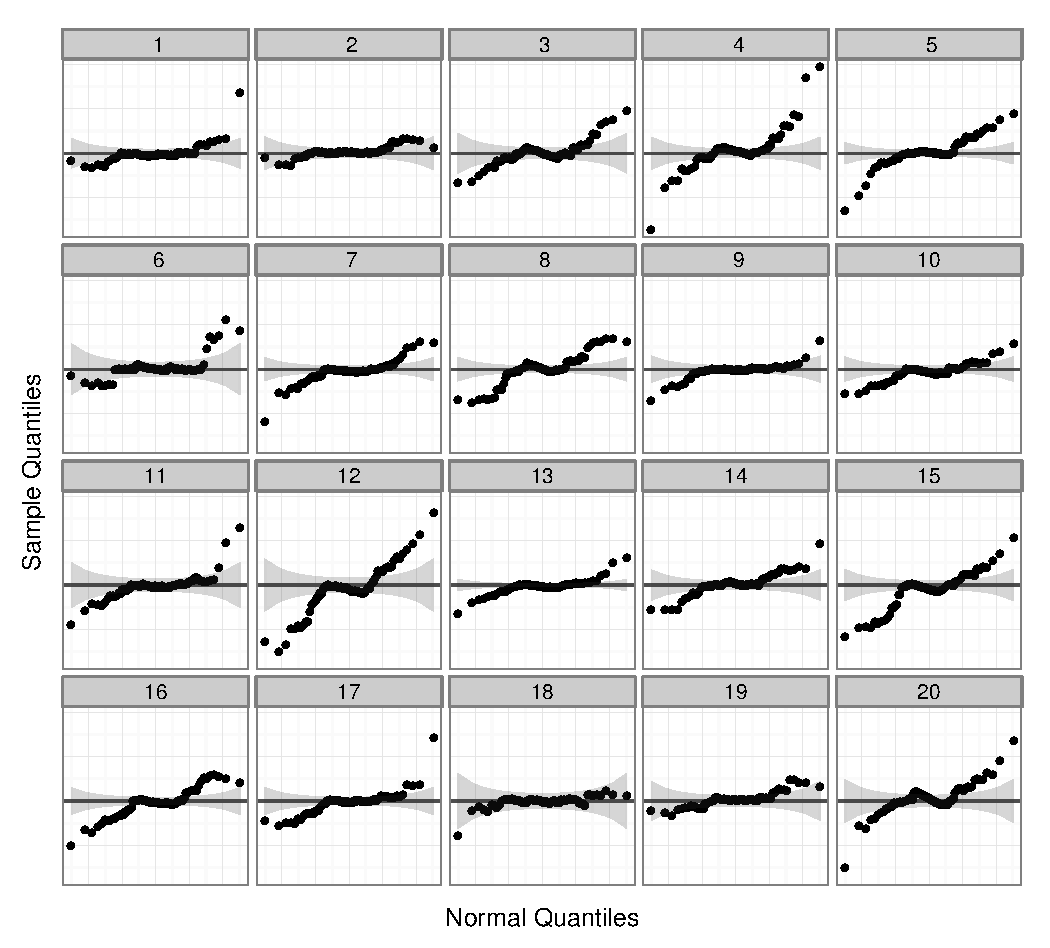
\includegraphics[width=0.9\textwidth]{qq-lineup-rot.pdf}%test.jpeg}%lineup-rslope.pdf}
	\caption{\label{fig:lineup-2} Lineup of detrended Q-Q plots for the random slope term in model~(1) from the paper. This plot shows the same data as the standard Q-Q plots in the paper. Out of 22 evaluations, 11 participants picked panel \#$(3^2+3)$ as the most different from the set; another 4 participants chose panel \#$(2 \cdot 3^2)$. None of the participant picked the panel of the observed data.}
\end{figure}

\begin{table}[ht]
% latex table generated in R 3.1.0 by xtable 1.7-3 package
% Wed Jul 30 15:49:14 2014
\centering
\begin{tabular}{rrrrrrrrrrr}
  \hline
  & \multicolumn{9}{l}{response} \\
Q-Q type & 2 & 3 & 4 & 5 & 6 & 11 & 12 & 15 & 18 & 20 \\ 
  \hline
  Standard & 0 & 0 & 2 & 1 & 2 & 1 & 15 & 4 & 0 & 2 \\ 
  Detrended & 1 & 1 & 1 & 1 & 0 & 0 & 11 & 2 & 4 & 1 \\ 
   \hline
\end{tabular}
\caption{\label{tab:lpresults}Overview of user picks evaluating lineups in figures~\ref{fig:lineup} and \ref{fig:lineup-2} for the panel with the most pronounced difference. Both standard and detrended version of Q-Q plots show similar results with a definite preference for panel \#12.}
\end{table}



\section{Evaluations of existing proposals}\label{supp:evals}
%--------------------------------------------------

\subsection{Model notation}
%--------------------------
Recall that the stacked representation of the hierarchical linear model is given by 
%
\begin{align}\label{eq:hlm}
	\underset{(n \times 1)}{\bm{y}} &= \underset{(n \times p)}{\bm{X}} \ \underset{(p \times 1)}{\bm{\beta}} + \underset{(n \times q)}{\bm{Z}} \ \underset{(q \times 1)}{\bm{b}} + \underset{(n \times 1)}{\bm{\varepsilon}},\\
	\bm{\varepsilon} & \overset{\text{iid}}{\sim} \mathcal{N}(\bm{0}, \ \bm{R}), \qquad \bm{b} \overset{\text{iid}}{\sim} \mathcal{N}(\bm{0},\ \bm{D}) \nonumber
\end{align}
%
where $\bm{y}$ is a vector of responses, $\bm{X}$ and $\bm{Z}$ are design matrices for the fixed and random effects, respectively, $\bm{\beta}$ is a vector of fixed effects, $\bm{b}$ is a vector of random effects, $\bm{\varepsilon}$ is a vector of error terms, and $\bm{R}$ and $\bm{D}$ are positive definite covariance matrices. Further, we assume that $\cov(\bm{\varepsilon},\ \bm{b}) = \bm{0}$. The above assumptions imply that, marginally, $\bm{y} \sim \mathcal{N}(\bm{X\beta},\ \bm{V})$ where $\bm{V} = \bm{ZDZ}\trans + \bm{R}$.

\subsection{Residuals}

In this section we consider residuals that are commonly used to check the distributional assumptions in a hierarchical linear model. For more general discussions of residual analysis for hierarchical linear models we refer the reader to \cite{Haslett:2007vv} and \cite{Nobre:2007ej}.

\paragraph{Marginal residuals.} 
%-----------------------------
The marginal distribution of $\bm{y}$ leads to the marginal residuals which are defined as
%
\begin{equation}\label{eq:marginalresid}
\widehat{\bm{\zeta}}  = \bm{y} - \bm{X} \widehat{\bm{\beta}} =  \bm{V P y}
\end{equation}
%
where $ \bm{P} = \bm{V\inv} - \bm{V\inv X} \left( \bm{X\trans V\inv X} \right) \bm{X \trans V\inv}$, and reveal how the observations deviate from the global trend. The use of these residuals for distributional assessment provides an omnibus assessment of goodness-of-fit as the marginal residuals are a linear combination of the other residual quantities; however, this assessment requires the empirical distribution of the marginal residuals to resemble true distribution. Asymptotically, the variance of the marginal residuals is $\var(\widehat{\zeta}) = \bm{V}$ leading to correlated residuals. To obtain asymptotically uncorrelated residuals the marginal residuals can be scaled by the Cholesky root of $\bm{V}$ \citep{Houseman:2004gq}, $\bm{C}$, yielding
%
\begin{equation}\label{eq:choleskyresid}
\bm{z}_{\zeta}  = \bm{C}\inv \widehat{\bm{\zeta}}
\end{equation}
%


\paragraph{Level-1 residuals.}
%-----------------------------
The distribution of $\bm{y}$ conditional on the random effects, $\bm{b}$, is given by
%
\begin{equation}\label{eq:marginalmodel}
	\bm{y} | \bm{b} \sim \mathcal{N}( \bm{X\beta} + \bm{Zb},\ \bm{R} ),
\end{equation}
%
and leads to the level-1 residuals, commonly referred to as the error terms, which are defined as
%
\begin{equation}\label{eq:lev1resid}
	\widehat{\bm{\varepsilon}} = \bm{y} - \bm{X \widehat{\beta}} + \bm{Z \widehat{b}} = \bm{R P y}
\end{equation}
%
and reveal the deviations of the observations from the conditional model. The variance of the level-1 residuals is given by $\var(\widehat{\bm{\varepsilon}}) = \bm{ R P R }$, so studentized level-1 residuals can be obtained by 
%
\begin{equation}\label{eq:lev1-std}
\bm{z}_{\varepsilon} =  \text{diag} \left(\bm{RPR} \right)^{-1/2} \widehat{\bm{\varepsilon}}
\end{equation}
%
which have been recommended for distributional assessment \citep{Nobre:2007ej}. An alternative approach is recommended by \citet[Section 4.3]{Pinhiero:2000vf} uses the Pearson residuals, which are obtained by dividing the predicted residuals by the estimated within-group standard deviation, $\widehat{\sigma}_\varepsilon$. 



\paragraph{Level-2 residuals.}
%-----------------------------
The final type of residual we consider is the the best linear unbiased predictor (BLUP) of the random effects (i.e., predicted random effects), providing insight into the differences between the marginal (global) and conditional models. By definition, the BLUP of $\bm{b}$ is
%
\begin{equation}\label{eq:lev2resid}
\widehat{\bm{b}} = \bm{D Z\trans V\inv} \left( \bm{y} - \bm{X \widehat{\beta}} \right) = \bm{D Z\trans P y}
\end{equation}
%
which has variance $\var(\widehat{\bm{b}}) = \bm{DZ\trans P ZD}$. 
%Rewriting $\var(\widehat{\bm{b}})$ as
%%
%\begin{equation}
%\bm{DZ\trans P ZD} = \bm{DZ\trans} \bm{V\inv} \left( \bm{V} - \bm{ X} \left( \bm{X\trans V\inv X} \right) \bm{X \trans} \right) \bm{V\inv} \bm{ZD}
%\end{equation}
%%
%leads to two 
For distributional assessment of the BLUPs it makes sense to examine each random effect individually, though \cite{Lange:1989uu} suggest the examination of linear combinations of standardized BLUPs. Rewritting the definition of $\var(\widehat{\bm{b}})$
%
\begin{equation}
\bm{DZ\trans P ZD} = \bm{DZ\trans} \bm{V\inv} \left( \bm{V} - \bm{ X} \left( \bm{X\trans V\inv X} \right) \bm{X \trans} \right) \bm{V\inv} \bm{ZD}
\end{equation}
%
leads to two similar standardizations of the BLUPs. The first utilizes the fact that when the number of groups is large $\bm{ X} \left( \bm{X\trans V\inv X} \right)$ will be small \citep{Goldstein:2011}, so for a large number of groups standardized BLUPs can be calculated by
%
\begin{equation}\label{eq:lev2-std1}
\bm{z}_{b} = \text{diag} \left(\bm{DZ\trans V\inv ZD}\right)^{-1/2} \widehat{\bm{b}}
\end{equation}
%
This formulation is the same used by \cite{Lange:1989uu} (discussed below).
%, who suggest creating weighted Q-Q plots \citep{Dempster:1985tr} to assess the distributional assumptions. Note that standardized linear combinations of the BLUPs follow in the usual way. 
The second standardization applies for all sample sizes and is given by
%
\begin{equation}\label{eq:lev2-std2}
\bm{z}_{b} = \text{diag} \left(\bm{DZ\trans P ZD}\right)^{-1/2} \widehat{\bm{b}}
\end{equation}
%


\subsection{Weighted Q-Q plots}
%------------------------------

As an alternative to Q-Q plots constructed from the BLUPs \cite{Lange:1989uu} propose using weighted Q-Q plots of standardized linear combinations of the BLUPs, $\bm{L\trans}\widehat{\bm{b}}$,
%
\begin{equation}
z_{b} = \text{diag} \left(\bm{L\trans DZ\trans V\inv ZDL}\right)^{-1/2} \bm{L\trans}\widehat{\bm{b}}
\end{equation}
%
The specific form of $\bm{L}$ chosen highlights different departures from distributional assumptions---for example, $\bm{L}$s can be chosen to extract the random slope and the random intercept terms individually. When the random effects may be correlated, \citeauthor{Lange:1989uu} suggest examining a range of additional linear combinations in-between the two marginal random effects either through manual specification of $\bm{L}$ or projection pursuit.
After choosing $\bm{L}$ a weighted Q-Q plot is constructed by comparing the weighted empirical cumulative distribution function
%
\begin{equation}
F_m^*(x) = \sum_{i=1}^{m} I(x - z_{b_i} \geq 0) w_i \bigg/ \sum_{i=1}^{m} w_i, 
\end{equation}
%
to $\Phi\inv \left ( F_m^*(z_{b_i}) \right)$. Here, $w_i$ is the $i$th element of $\bm{L\trans DZ\trans V\inv ZDL}$.
For balanced group sizes this simplifies to the unweighted Q-Q plot of $\bm{z}_b$.
%

\subsection{Simulation-based approaches}
%---------------------------------------

All of the above approaches to checking the distributional assumptions rely on the use of interrelated residuals, which has been reported to be problematic \citep{HildenMinton:1995wh, Verbeke:1996va}.  
One alternative that has been proposed to overcome this problem is the use of the parametric bootstrap to develop point-wise and simultaneous confidence bands for Q-Q plots. We evaluate the potential of this method using bootstrap tests of normality.


\subsection{Simulation study}\label{supp:simstudy1}
%--------------------------------------------------

To evaluate the above proposals we carried out a simulation study under the same settings as in the paper, with the only difference being that the original $\bm{Z}$ was used for data generation. To evaluate the bootstrap tests of normality, a null distribution of 5000 simulated test statistics for each situation was used.

Tables~\ref{tab:eval1}--\ref{tab:evalmarginal} present the results of using standard normality tests to assess the distributional assumptions of the residuals from a hierarchical model. The gray background on the table indicates which simulation settings estimate type I error, with the other rows estimating power. Tables~\ref{tab:boot1}--\ref{tab:bootmarginal} present the results of the bootstrap tests for normality. Table~\ref{tab:langeryan} presents the results of using a weighted CDF to evaluate the normality of the random effects, in this case the null distribution was obtained using the parametric bootstrap.

The simulation study reveals that none of the residual-based diagnostics for assessing distributional assumptions are appropriate in all situations. The error terms can be targeted either by the use of studentized residuals or a parametric bootstrap; however, the assessment of this assumption is less critical. The random effects, on which predictive inference relies, cannot be targeted by the current methods when the residual variance is larger than the variance component associated with the random effects---that is, situations with higher degrees of shrinkage.  Such situations are often encountered in practice. Additionally, use of the parametric bootstrap---to construct simulation envelopes for Q-Q plots, for example---does not appear to remedy this situation based on the performance of the bootstrap tests. Finally, we can see that \citeauthor{Lange:1989uu}'s weighted Q-Q plots cannot target the random effects distribution when the residual variance is large, as the distribution of the error terms overly influences tests for the random slope, resulting in inflated type I error rates for both random effects.

%&&&&&&&&&&&&&&&&&&&&&&&&&&&&&&&&&&&&&&&&&&&&&&&&&&&&&&&&&&&&&&&&&&&&&&&&&&&&&&
% Correct model
%&&&&&&&&&&&&&&&&&&&&&&&&&&&&&&&&&&&&&&&&&&&&&&&&&&&&&&&&&&&&&&&&&&&&&&&&&&&&&&


%------------------------------------------------
% Naive tests
%------------------------------------------------

%%% Level-1 residuals
\begin{table}[ht]
\centering
\caption{\label{tab:eval1} Proportion of tests rejecting the null hypothesis of normality of the error terms.}
\begin{scriptsize}
\begin{tabular}{ll p{.1cm} c p{.1cm} rrr p{.1cm} rrr p{.1cm} rrr}
  \hline
  \multicolumn{2}{c}{Distributions}& & Nominal & &  \multicolumn{3}{c}{Raw residuals} & & \multicolumn{3}{c}{Pearson residuals} & & \multicolumn{3}{c}{Studentized residuals}\\ \cline{1-2} \cline{6-8} \cline{10-12} \cline{14-16}
  Errors & Random effects & & $\alpha$ & & AD & CVM & KS & & AD & CVM & KS & & AD & CVM & KS \\ 
   \hline
& && && \multicolumn{9}{c}{$\sigma_{\varepsilon}^2 = 4$, \ \ $\sigma_{b_0}^2 = \sigma_{b_1}^2 = 1$} \\ \cline{6-16}

\rowcolor{gray!20} Normal       & Normal       && 0.05 && 0.07 & 0.06 & 0.06 && 0.07 & 0.06 & 0.06 && 0.04 & 0.04 & 0.04 \\ 
\rowcolor{gray!20}             &              && 0.10 && 0.13 & 0.12 & 0.12 && 0.13 & 0.12 & 0.12 && 0.09 & 0.09 & 0.10 \\ 
\rowcolor{gray!20}             & Heavy tailed && 0.05 && 0.07 & 0.08 & 0.06 && 0.07 & 0.08 & 0.06 && 0.05 & 0.05 & 0.05 \\ 
\rowcolor{gray!20}             &              && 0.10 && 0.14 & 0.13 & 0.14 && 0.14 & 0.13 & 0.14 && 0.11 & 0.11 & 0.10 \\ 
\rowcolor{gray!20}             & Skewed       && 0.05 && 0.07 & 0.06 & 0.06 && 0.07 & 0.06 & 0.06 && 0.04 & 0.04 & 0.05 \\ 
\rowcolor{gray!20}             &              && 0.10 && 0.13 & 0.12 & 0.13 && 0.13 & 0.12 & 0.13 && 0.09 & 0.09 & 0.10 \\ 
             &&&&&&&&&&&&&&&\\
Heavy tailed & Normal       && 0.05 && 1.00 & 1.00 & 1.00 && 1.00 & 1.00 & 1.00 && 1.00 & 1.00 & 1.00 \\ 
             &              && 0.10 && 1.00 & 1.00 & 1.00 && 1.00 & 1.00 & 1.00 && 1.00 & 1.00 & 1.00 \\ 
             & Heavy tailed && 0.05 && 1.00 & 1.00 & 1.00 && 1.00 & 1.00 & 1.00 && 1.00 & 1.00 & 1.00 \\ 
             &              && 0.10 && 1.00 & 1.00 & 1.00 && 1.00 & 1.00 & 1.00 && 1.00 & 1.00 & 1.00 \\ 
             & Skewed       && 0.05 && 1.00 & 1.00 & 1.00 && 1.00 & 1.00 & 1.00 && 1.00 & 1.00 & 1.00 \\ 
             &              && 0.10 && 1.00 & 1.00 & 1.00 && 1.00 & 1.00 & 1.00 && 1.00 & 1.00 & 1.00 \\ 
             &&&&&&&&&&&&&&&\\
Skewed       & Normal       && 0.05 && 1.00 & 1.00 & 1.00 && 1.00 & 1.00 & 1.00 && 1.00 & 1.00 & 1.00 \\ 
             &              && 0.10 && 1.00 & 1.00 & 1.00 && 1.00 & 1.00 & 1.00 && 1.00 & 1.00 & 1.00 \\ 
             & Heavy tailed && 0.05 && 1.00 & 1.00 & 1.00 && 1.00 & 1.00 & 1.00 && 1.00 & 1.00 & 1.00 \\ 
             &              && 0.10 && 1.00 & 1.00 & 1.00 && 1.00 & 1.00 & 1.00 && 1.00 & 1.00 & 1.00 \\ 
             & Skewed       && 0.05 && 1.00 & 1.00 & 1.00 && 1.00 & 1.00 & 1.00 && 1.00 & 1.00 & 1.00 \\ 
             &              && 0.10 && 1.00 & 1.00 & 1.00 && 1.00 & 1.00 & 1.00 && 1.00 & 1.00 & 1.00 \\ 

&&&&&&&&&&&&&&&\\
& && && \multicolumn{9}{c}{$\sigma_{\varepsilon}^2 = 1$, \ \ $\sigma_{b_0}^2 = \sigma_{b_1}^2 = 1$} \\ \cline{6-16}

\rowcolor{gray!20} Normal       & Normal       && 0.05 &&  0.05 & 0.05 & 0.04 && 0.05 & 0.05 & 0.04 && 0.04 & 0.04 & 0.04 \\ 
\rowcolor{gray!20}              &              && 0.10 &&  0.11 & 0.10 & 0.09 && 0.11 & 0.10 & 0.09 && 0.09 & 0.09 & 0.08 \\ 
\rowcolor{gray!20}              & Heavy tailed && 0.05 &&  0.07 & 0.06 & 0.06 && 0.07 & 0.06 & 0.06 && 0.05 & 0.06 & 0.05 \\ 
\rowcolor{gray!20}              &              && 0.10 &&  0.13 & 0.12 & 0.11 && 0.13 & 0.12 & 0.11 && 0.11 & 0.11 & 0.10 \\ 
\rowcolor{gray!20}              & Skewed       && 0.05 &&  0.05 & 0.05 & 0.05 && 0.05 & 0.05 & 0.05 && 0.04 & 0.04 & 0.04 \\ 
\rowcolor{gray!20}              &              && 0.10 &&  0.10 & 0.09 & 0.11 && 0.10 & 0.09 & 0.11 && 0.08 & 0.09 & 0.10 \\ 
              &&&&&&&&&&&&&&&\\
 Heavy tailed & Normal       && 0.05 &&  1.00 & 1.00 & 1.00 && 1.00 & 1.00 & 1.00 && 1.00 & 1.00 & 1.00 \\ 
              &              && 0.10 &&  1.00 & 1.00 & 1.00 && 1.00 & 1.00 & 1.00 && 1.00 & 1.00 & 1.00 \\ 
              & Heavy tailed && 0.05 &&  1.00 & 1.00 & 1.00 && 1.00 & 1.00 & 1.00 && 1.00 & 1.00 & 1.00 \\ 
              &              && 0.10 &&  1.00 & 1.00 & 1.00 && 1.00 & 1.00 & 1.00 && 1.00 & 1.00 & 1.00 \\ 
              & Skewed       && 0.05 &&  1.00 & 1.00 & 1.00 && 1.00 & 1.00 & 1.00 && 1.00 & 1.00 & 1.00 \\ 
              &              && 0.10 &&  1.00 & 1.00 & 1.00 && 1.00 & 1.00 & 1.00 && 1.00 & 1.00 & 1.00 \\ 
              &&&&&&&&&&&&&&&\\
 Skewed       & Normal       && 0.05 &&  1.00 & 1.00 & 1.00 && 1.00 & 1.00 & 1.00 && 1.00 & 1.00 & 1.00 \\ 
              &              && 0.10 &&  1.00 & 1.00 & 1.00 && 1.00 & 1.00 & 1.00 && 1.00 & 1.00 & 1.00 \\ 
              & Heavy tailed && 0.05 &&  1.00 & 1.00 & 1.00 && 1.00 & 1.00 & 1.00 && 1.00 & 1.00 & 1.00 \\ 
              &              && 0.10 &&  1.00 & 1.00 & 1.00 && 1.00 & 1.00 & 1.00 && 1.00 & 1.00 & 1.00 \\ 
              & Skewed       && 0.05 &&  1.00 & 1.00 & 1.00 && 1.00 & 1.00 & 1.00 && 1.00 & 1.00 & 1.00 \\ 
              &              && 0.10 &&  1.00 & 1.00 & 1.00 && 1.00 & 1.00 & 1.00 && 1.00 & 1.00 & 1.00 \\ 

&&&&&&&&&&&&&&&\\
& && && \multicolumn{9}{c}{$\sigma_{\varepsilon}^2 = 1$, \ \ $\sigma_{b_0}^2 = \sigma_{b_1}^2 = 4$} \\ \cline{6-16}

\rowcolor{gray!20} Normal       & Normal       && 0.05 &&  0.10 & 0.09 & 0.07 && 0.10 & 0.09 & 0.07 && 0.05 & 0.04 & 0.04 \\ 
\rowcolor{gray!20}             &              && 0.10 &&  0.17 & 0.17 & 0.15 && 0.17 & 0.17 & 0.15 && 0.09 & 0.09 & 0.09 \\ 
\rowcolor{gray!20}             & Heavy tailed && 0.05 &&  0.11 & 0.11 & 0.10 && 0.11 & 0.11 & 0.10 && 0.06 & 0.06 & 0.05 \\ 
\rowcolor{gray!20}             &              && 0.10 &&  0.19 & 0.19 & 0.19 && 0.19 & 0.19 & 0.19 && 0.12 & 0.11 & 0.12 \\ 
\rowcolor{gray!20}             & Skewed       && 0.05 &&  0.10 & 0.10 & 0.09 && 0.10 & 0.10 & 0.09 && 0.05 & 0.05 & 0.06 \\ 
\rowcolor{gray!20}             &              && 0.10 &&  0.18 & 0.18 & 0.17 && 0.18 & 0.18 & 0.17 && 0.11 & 0.11 & 0.11 \\ 
             &&&&&&&&&&&&&&&\\
Heavy tailed & Normal       && 0.05 &&  1.00 & 1.00 & 1.00 && 1.00 & 1.00 & 1.00 && 1.00 & 1.00 & 1.00 \\ 
             &              && 0.10 &&  1.00 & 1.00 & 1.00 && 1.00 & 1.00 & 1.00 && 1.00 & 1.00 & 1.00 \\ 
             & Heavy tailed && 0.05 &&  1.00 & 1.00 & 1.00 && 1.00 & 1.00 & 1.00 && 1.00 & 1.00 & 1.00 \\ 
             &              && 0.10 &&  1.00 & 1.00 & 1.00 && 1.00 & 1.00 & 1.00 && 1.00 & 1.00 & 1.00 \\ 
             & Skewed       && 0.05 &&  1.00 & 1.00 & 1.00 && 1.00 & 1.00 & 1.00 && 1.00 & 1.00 & 1.00 \\ 
             &              && 0.10 &&  1.00 & 1.00 & 1.00 && 1.00 & 1.00 & 1.00 && 1.00 & 1.00 & 1.00 \\ 
             &&&&&&&&&&&&&&&\\
Skewed       & Normal       && 0.05 &&  1.00 & 1.00 & 1.00 && 1.00 & 1.00 & 1.00 && 1.00 & 1.00 & 1.00 \\ 
             &              && 0.10 &&  1.00 & 1.00 & 1.00 && 1.00 & 1.00 & 1.00 && 1.00 & 1.00 & 1.00 \\ 
             & Heavy tailed && 0.05 &&  1.00 & 1.00 & 1.00 && 1.00 & 1.00 & 1.00 && 1.00 & 1.00 & 1.00 \\ 
             &              && 0.10 &&  1.00 & 1.00 & 1.00 && 1.00 & 1.00 & 1.00 && 1.00 & 1.00 & 1.00 \\ 
             & Skewed       && 0.05 &&  1.00 & 1.00 & 1.00 && 1.00 & 1.00 & 1.00 && 1.00 & 1.00 & 1.00 \\ 
             &              && 0.10 &&  1.00 & 1.00 & 1.00 && 1.00 & 1.00 & 1.00 && 1.00 & 1.00 & 1.00 \\ 


   \hline
\end{tabular}
\end{scriptsize}
\end{table}

%%% Level-2 residuals
\begin{table}[ht]
\centering
\caption{\label{tab:evalb0} Proportion of tests rejecting the null hypothesis of normality of the random intercept.}
\begin{scriptsize}
\begin{tabular}{ll p{.1cm} c p{.1cm} rrr p{.1cm} rrr p{.1cm} rrr}
  \hline
  \multicolumn{2}{c}{Distributions}& & Nominal & &  \multicolumn{3}{c}{Raw residuals} & & \multicolumn{3}{c}{Pearson residuals} & & \multicolumn{3}{c}{Studentized residuals}\\ \cline{1-2} \cline{6-8} \cline{10-12} \cline{14-16}
  Random effects & Errors & & $\alpha$ & & AD & CVM & KS & & AD & CVM & KS & & AD & CVM & KS \\ 
   \hline
& && && \multicolumn{9}{c}{$\sigma_{\varepsilon}^2 = 4$, \ \ $\sigma_{b_0}^2 = \sigma_{b_1}^2 = 1$} \\ \cline{6-16}

\rowcolor{gray!20} Normal       & Normal       && 0.05 &&   0.05 & 0.05 & 0.05 && 0.05 & 0.05 & 0.06 && 0.05 & 0.05 & 0.06 \\ 
\rowcolor{gray!20}             &              && 0.10 &&   0.10 & 0.10 & 0.10 && 0.11 & 0.10 & 0.12 && 0.11 & 0.10 & 0.12 \\ 
\rowcolor{gray!20}             & Heavy tailed && 0.05 &&   0.15 & 0.13 & 0.12 && 0.17 & 0.15 & 0.13 && 0.17 & 0.15 & 0.13 \\ 
\rowcolor{gray!20}             &              && 0.10 &&   0.22 & 0.20 & 0.20 && 0.26 & 0.23 & 0.21 && 0.26 & 0.23 & 0.20 \\ 
\rowcolor{gray!20}             & Skewed       && 0.05 &&   0.16 & 0.15 & 0.13 && 0.18 & 0.17 & 0.14 && 0.18 & 0.17 & 0.14 \\ 
\rowcolor{gray!20}             &              && 0.10 &&   0.25 & 0.23 & 0.21 && 0.28 & 0.25 & 0.22 && 0.28 & 0.25 & 0.21 \\ 
             &&&&&&&&&&&&&&&\\
Heavy tailed & Normal       && 0.05 &&   0.27 & 0.24 & 0.19 && 0.28 & 0.26 & 0.21 && 0.28 & 0.26 & 0.21 \\ 
             &              && 0.10 &&   0.35 & 0.31 & 0.28 && 0.36 & 0.34 & 0.30 && 0.36 & 0.33 & 0.30 \\ 
             & Heavy tailed && 0.05 &&   0.49 & 0.45 & 0.35 && 0.51 & 0.46 & 0.36 && 0.50 & 0.46 & 0.36 \\ 
             &              && 0.10 &&   0.58 & 0.54 & 0.46 && 0.60 & 0.55 & 0.47 && 0.60 & 0.55 & 0.47 \\ 
             & Skewed       && 0.05 &&   0.52 & 0.48 & 0.36 && 0.55 & 0.50 & 0.40 && 0.55 & 0.50 & 0.40 \\ 
             &              && 0.10 &&   0.62 & 0.59 & 0.51 && 0.65 & 0.60 & 0.53 && 0.65 & 0.60 & 0.52 \\
             &&&&&&&&&&&&&&&\\ 
Skewed       & Normal       && 0.05 &&   0.51 & 0.48 & 0.39 && 0.51 & 0.49 & 0.38 && 0.51 & 0.49 & 0.39 \\ 
             &              && 0.10 &&   0.61 & 0.58 & 0.51 && 0.61 & 0.59 & 0.52 && 0.60 & 0.58 & 0.52 \\ 
             & Heavy tailed && 0.05 &&   0.73 & 0.69 & 0.58 && 0.73 & 0.70 & 0.59 && 0.73 & 0.70 & 0.59 \\ 
             &              && 0.10 &&   0.80 & 0.77 & 0.69 && 0.81 & 0.78 & 0.70 && 0.80 & 0.78 & 0.70 \\ 
             & Skewed       && 0.05 &&   0.87 & 0.83 & 0.70 && 0.87 & 0.82 & 0.69 && 0.86 & 0.83 & 0.69 \\ 
             &              && 0.10 &&   0.92 & 0.89 & 0.80 && 0.91 & 0.88 & 0.80 && 0.91 & 0.88 & 0.80 \\ 

&&&&&&&&&&&&&&&\\
& && && \multicolumn{9}{c}{$\sigma_{\varepsilon}^2 = 1$, \ \ $\sigma_{b_0}^2 = \sigma_{b_1}^2 = 1$} \\ \cline{6-16}
\rowcolor{gray!20} Normal       & Normal       && 0.05 &&   0.05 & 0.05 & 0.04 && 0.05 & 0.05 & 0.04 && 0.05 & 0.05 & 0.04 \\ 
\rowcolor{gray!20}             &              && 0.10 &&   0.09 & 0.09 & 0.08 && 0.09 & 0.08 & 0.08 && 0.08 & 0.08 & 0.08 \\ 
\rowcolor{gray!20}             & Heavy tailed && 0.05 &&   0.07 & 0.07 & 0.06 && 0.07 & 0.07 & 0.06 && 0.07 & 0.07 & 0.06 \\ 
\rowcolor{gray!20}             &              && 0.10 &&   0.12 & 0.12 & 0.11 && 0.12 & 0.11 & 0.11 && 0.12 & 0.11 & 0.11 \\ 
\rowcolor{gray!20}             & Skewed       && 0.05 &&   0.06 & 0.06 & 0.07 && 0.06 & 0.06 & 0.06 && 0.06 & 0.06 & 0.06 \\ 
\rowcolor{gray!20}             &              && 0.10 &&   0.11 & 0.11 & 0.12 && 0.12 & 0.12 & 0.12 && 0.12 & 0.11 & 0.12 \\
             &&&&&&&&&&&&&&&\\  
Heavy tailed & Normal       && 0.05 &&   0.55 & 0.50 & 0.42 && 0.52 & 0.48 & 0.40 && 0.52 & 0.48 & 0.40 \\ 
             &              && 0.10 &&   0.63 & 0.60 & 0.51 && 0.60 & 0.56 & 0.51 && 0.60 & 0.56 & 0.52 \\ 
             & Heavy tailed && 0.05 &&   0.63 & 0.58 & 0.49 && 0.60 & 0.56 & 0.47 && 0.60 & 0.56 & 0.47 \\ 
             &              && 0.10 &&   0.71 & 0.68 & 0.60 && 0.68 & 0.63 & 0.56 && 0.68 & 0.63 & 0.56 \\ 
             & Skewed       && 0.05 &&   0.62 & 0.57 & 0.47 && 0.61 & 0.55 & 0.46 && 0.61 & 0.55 & 0.46 \\ 
             &              && 0.10 &&   0.71 & 0.66 & 0.58 && 0.69 & 0.65 & 0.57 && 0.69 & 0.64 & 0.57 \\ 
             &&&&&&&&&&&&&&&\\ 
Skewed       & Normal       && 0.05 &&   0.93 & 0.92 & 0.86 && 0.93 & 0.91 & 0.86 && 0.93 & 0.91 & 0.85 \\ 
             &              && 0.10 &&   0.96 & 0.94 & 0.91 && 0.96 & 0.94 & 0.90 && 0.95 & 0.94 & 0.90 \\ 
             & Heavy tailed && 0.05 &&   0.97 & 0.96 & 0.89 && 0.97 & 0.96 & 0.88 && 0.97 & 0.96 & 0.88 \\ 
             &              && 0.10 &&   0.99 & 0.98 & 0.94 && 0.99 & 0.98 & 0.94 && 0.99 & 0.98 & 0.94 \\ 
             & Skewed       && 0.05 &&   0.98 & 0.96 & 0.90 && 0.98 & 0.97 & 0.90 && 0.98 & 0.97 & 0.91 \\ 
             &              && 0.10 &&   0.99 & 0.97 & 0.95 && 0.99 & 0.98 & 0.94 && 0.99 & 0.98 & 0.95 \\ 


&&&&&&&&&&&&&&&\\
& && && \multicolumn{9}{c}{$\sigma_{\varepsilon}^2 = 1$, \ \ $\sigma_{b_0}^2 = \sigma_{b_1}^2 = 4$} \\ \cline{6-16}

\rowcolor{gray!20} Normal       & Normal       && 0.05 &&  0.05 & 0.05 & 0.05 && 0.05 & 0.05 & 0.04 && 0.05 & 0.05 & 0.04 \\ 
\rowcolor{gray!20}             &              && 0.10 &&  0.10 & 0.09 & 0.09 && 0.10 & 0.09 & 0.09 && 0.10 & 0.09 & 0.09 \\ 
\rowcolor{gray!20}             & Heavy tailed && 0.05 &&  0.04 & 0.04 & 0.05 && 0.05 & 0.05 & 0.05 && 0.05 & 0.05 & 0.05 \\ 
\rowcolor{gray!20}             &              && 0.10 &&  0.09 & 0.09 & 0.09 && 0.09 & 0.09 & 0.09 && 0.09 & 0.09 & 0.09 \\ 
\rowcolor{gray!20}             & Skewed       && 0.05 &&  0.04 & 0.04 & 0.03 && 0.04 & 0.04 & 0.03 && 0.04 & 0.04 & 0.03 \\ 
\rowcolor{gray!20}             &              && 0.10 &&  0.09 & 0.09 & 0.08 && 0.10 & 0.09 & 0.08 && 0.09 & 0.09 & 0.08 \\ 
             &&&&&&&&&&&&&&&\\
Heavy tailed & Normal       && 0.05 &&  0.68 & 0.63 & 0.54 && 0.68 & 0.63 & 0.54 && 0.68 & 0.63 & 0.54 \\ 
             &              && 0.10 &&  0.75 & 0.71 & 0.63 && 0.75 & 0.70 & 0.64 && 0.75 & 0.71 & 0.64 \\ 
             & Heavy tailed && 0.05 &&  0.71 & 0.67 & 0.57 && 0.71 & 0.67 & 0.58 && 0.71 & 0.67 & 0.57 \\ 
             &              && 0.10 &&  0.78 & 0.76 & 0.68 && 0.79 & 0.76 & 0.67 && 0.79 & 0.75 & 0.67 \\ 
             & Skewed       && 0.05 &&  0.70 & 0.68 & 0.57 && 0.70 & 0.67 & 0.56 && 0.70 & 0.67 & 0.56 \\ 
             &              && 0.10 &&  0.78 & 0.74 & 0.68 && 0.78 & 0.74 & 0.68 && 0.78 & 0.74 & 0.67 \\ 
             &&&&&&&&&&&&&&&\\
Skewed       & Normal       && 0.05 &&  1.00 & 0.99 & 0.97 && 1.00 & 0.99 & 0.97 && 1.00 & 0.99 & 0.97 \\ 
             &              && 0.10 &&  1.00 & 1.00 & 0.99 && 1.00 & 1.00 & 0.99 && 1.00 & 1.00 & 0.99 \\ 
             & Heavy tailed && 0.05 &&  1.00 & 1.00 & 0.98 && 1.00 & 1.00 & 0.98 && 1.00 & 1.00 & 0.98 \\ 
             &              && 0.10 &&  1.00 & 1.00 & 0.99 && 1.00 & 1.00 & 0.99 && 1.00 & 1.00 & 0.99 \\ 
             & Skewed       && 0.05 &&  1.00 & 1.00 & 0.98 && 1.00 & 1.00 & 0.98 && 1.00 & 1.00 & 0.98 \\ 
             &              && 0.10 &&  1.00 & 1.00 & 0.99 && 1.00 & 1.00 & 0.99 && 1.00 & 1.00 & 0.99 \\ 


   \hline
\end{tabular}
\end{scriptsize}
\end{table}


\begin{table}[ht]
\centering
\caption{\label{tab:evalb1} Proportion of tests rejecting the null hypothesis of normality of the random slope.}
\begin{scriptsize}
\begin{tabular}{ll p{.1cm} c p{.1cm} rrr p{.1cm} rrr p{.1cm} rrr}
  \hline
  \multicolumn{2}{c}{Distributions}& & Nominal & &  \multicolumn{3}{c}{Raw residuals} & & \multicolumn{3}{c}{Pearson residuals} & & \multicolumn{3}{c}{Studentized residuals}\\ \cline{1-2} \cline{6-8} \cline{10-12} \cline{14-16}
  Random effects & Errors & & $\alpha$ & & AD & CVM & KS & & AD & CVM & KS & & AD & CVM & KS \\ 
   \hline
& && && \multicolumn{9}{c}{$\sigma_{\varepsilon}^2 = 4$, \ \ $\sigma_{b_0}^2 = \sigma_{b_1}^2 = 1$} \\ \cline{6-16}

\rowcolor{gray!20} Normal       & Normal       && 0.05 &&   1.00 & 1.00 & 1.00 && 0.05 & 0.05 & 0.06 && 0.05 & 0.05 & 0.06 \\ 
\rowcolor{gray!20}             &              && 0.10 &&   1.00 & 1.00 & 1.00 && 0.10 & 0.10 & 0.10 && 0.10 & 0.10 & 0.10 \\ 
\rowcolor{gray!20}             & Heavy tailed && 0.05 &&   1.00 & 1.00 & 1.00 && 0.26 & 0.24 & 0.19 && 0.26 & 0.24 & 0.19 \\ 
\rowcolor{gray!20}             &              && 0.10 &&   1.00 & 1.00 & 1.00 && 0.35 & 0.32 & 0.27 && 0.35 & 0.32 & 0.27 \\ 
\rowcolor{gray!20}             & Skewed       && 0.05 &&   1.00 & 1.00 & 1.00 && 0.33 & 0.31 & 0.24 && 0.33 & 0.31 & 0.24 \\ 
\rowcolor{gray!20}             &              && 0.10 &&   1.00 & 1.00 & 1.00 && 0.41 & 0.38 & 0.34 && 0.41 & 0.38 & 0.34 \\ 
             &&&&&&&&&&&&&&&\\
Heavy tailed & Normal       && 0.05 &&   1.00 & 1.00 & 1.00 && 0.13 & 0.12 & 0.09 && 0.13 & 0.12 & 0.09 \\ 
             &              && 0.10 &&   1.00 & 1.00 & 1.00 && 0.18 & 0.19 & 0.17 && 0.18 & 0.19 & 0.17 \\ 
             & Heavy tailed && 0.05 &&   1.00 & 1.00 & 1.00 && 0.40 & 0.36 & 0.29 && 0.40 & 0.36 & 0.29 \\ 
             &              && 0.10 &&   1.00 & 1.00 & 1.00 && 0.49 & 0.44 & 0.37 && 0.49 & 0.45 & 0.37 \\ 
             & Skewed       && 0.05 &&   1.00 & 1.00 & 1.00 && 0.49 & 0.46 & 0.37 && 0.49 & 0.46 & 0.37 \\ 
             &              && 0.10 &&   1.00 & 1.00 & 1.00 && 0.59 & 0.56 & 0.50 && 0.59 & 0.56 & 0.49 \\
             &&&&&&&&&&&&&&&\\ 
Skewed       & Normal       && 0.05 &&   1.00 & 1.00 & 1.00 && 0.12 & 0.11 & 0.10 && 0.12 & 0.11 & 0.10 \\ 
             &              && 0.10 &&   1.00 & 1.00 & 1.00 && 0.17 & 0.16 & 0.16 && 0.18 & 0.16 & 0.16 \\ 
             & Heavy tailed && 0.05 &&   1.00 & 1.00 & 1.00 && 0.41 & 0.37 & 0.30 && 0.40 & 0.37 & 0.30 \\ 
             &              && 0.10 &&   1.00 & 1.00 & 1.00 && 0.51 & 0.47 & 0.39 && 0.51 & 0.47 & 0.39 \\ 
             & Skewed       && 0.05 &&   1.00 & 1.00 & 1.00 && 0.59 & 0.56 & 0.46 && 0.59 & 0.56 & 0.46 \\ 
             &              && 0.10 &&   1.00 & 1.00 & 1.00 && 0.70 & 0.66 & 0.58 && 0.70 & 0.66 & 0.58 \\ 

&&&&&&&&&&&&&&&\\
& && && \multicolumn{9}{c}{$\sigma_{\varepsilon}^2 = 1$, \ \ $\sigma_{b_0}^2 = \sigma_{b_1}^2 = 1$} \\ \cline{6-16}

\rowcolor{gray!20} Normal       & Normal       && 0.05 &&  1.00 & 1.00 & 1.00 && 0.05 & 0.05 & 0.06 && 0.05 & 0.05 & 0.06 \\ 
\rowcolor{gray!20}             &              && 0.10 &&  1.00 & 1.00 & 1.00 && 0.12 & 0.11 & 0.11 && 0.12 & 0.11 & 0.11 \\ 
\rowcolor{gray!20}             & Heavy tailed && 0.05 &&  1.00 & 1.00 & 1.00 && 0.13 & 0.12 & 0.11 && 0.13 & 0.12 & 0.11 \\ 
\rowcolor{gray!20}             &              && 0.10 &&  1.00 & 1.00 & 1.00 && 0.22 & 0.20 & 0.17 && 0.22 & 0.20 & 0.17 \\ 
\rowcolor{gray!20}             & Skewed       && 0.05 &&  1.00 & 1.00 & 1.00 && 0.14 & 0.12 & 0.10 && 0.14 & 0.12 & 0.11 \\ 
\rowcolor{gray!20}             &              && 0.10 &&  1.00 & 1.00 & 1.00 && 0.22 & 0.20 & 0.17 && 0.22 & 0.20 & 0.17 \\
             &&&&&&&&&&&&&&&\\ 
Heavy tailed & Normal       && 0.05 &&  1.00 & 1.00 & 1.00 && 0.27 & 0.24 & 0.19 && 0.27 & 0.24 & 0.19 \\ 
             &              && 0.10 &&  1.00 & 1.00 & 1.00 && 0.35 & 0.32 & 0.27 && 0.35 & 0.31 & 0.27 \\ 
             & Heavy tailed && 0.05 &&  1.00 & 1.00 & 1.00 && 0.44 & 0.40 & 0.33 && 0.44 & 0.40 & 0.33 \\ 
             &              && 0.10 &&  1.00 & 1.00 & 1.00 && 0.50 & 0.48 & 0.42 && 0.50 & 0.48 & 0.42 \\ 
             & Skewed       && 0.05 &&  1.00 & 1.00 & 1.00 && 0.41 & 0.38 & 0.31 && 0.41 & 0.38 & 0.31 \\ 
             &              && 0.10 &&  1.00 & 1.00 & 1.00 && 0.51 & 0.48 & 0.42 && 0.51 & 0.48 & 0.42 \\ 
             &&&&&&&&&&&&&&&\\
Skewed       & Normal       && 0.05 &&  1.00 & 1.00 & 1.00 && 0.46 & 0.42 & 0.34 && 0.46 & 0.42 & 0.34 \\ 
             &              && 0.10 &&  1.00 & 1.00 & 1.00 && 0.57 & 0.52 & 0.46 && 0.57 & 0.52 & 0.46 \\ 
             & Heavy tailed && 0.05 &&  1.00 & 1.00 & 1.00 && 0.65 & 0.60 & 0.51 && 0.65 & 0.60 & 0.51 \\ 
             &              && 0.10 &&  1.00 & 1.00 & 1.00 && 0.73 & 0.69 & 0.62 && 0.73 & 0.69 & 0.62 \\ 
             & Skewed       && 0.05 &&  1.00 & 1.00 & 1.00 && 0.75 & 0.70 & 0.57 && 0.75 & 0.70 & 0.57 \\ 
             &              && 0.10 &&  1.00 & 1.00 & 1.00 && 0.83 & 0.78 & 0.70 && 0.83 & 0.78 & 0.70 \\ 


&&&&&&&&&&&&&&&\\
& && && \multicolumn{9}{c}{$\sigma_{\varepsilon}^2 = 1$, \ \ $\sigma_{b_0}^2 = \sigma_{b_1}^2 = 4$} \\ \cline{6-16}

\rowcolor{gray!20} Normal       & Normal       && 0.05 &&  1.00 & 1.00 & 1.00 && 0.04 & 0.05 & 0.05 && 0.04 & 0.05 & 0.05 \\ 
\rowcolor{gray!20}             &              && 0.10 &&  1.00 & 1.00 & 1.00 && 0.11 & 0.10 & 0.10 && 0.11 & 0.10 & 0.10 \\ 
\rowcolor{gray!20}             & Heavy tailed && 0.05 &&  1.00 & 1.00 & 1.00 && 0.07 & 0.07 & 0.07 && 0.07 & 0.07 & 0.07 \\ 
\rowcolor{gray!20}             &              && 0.10 &&  1.00 & 1.00 & 1.00 && 0.12 & 0.12 & 0.13 && 0.12 & 0.12 & 0.13 \\ 
\rowcolor{gray!20}             & Skewed       && 0.05 &&  1.00 & 1.00 & 1.00 && 0.06 & 0.06 & 0.05 && 0.06 & 0.06 & 0.05 \\ 
\rowcolor{gray!20}             &              && 0.10 &&  1.00 & 1.00 & 1.00 && 0.11 & 0.11 & 0.11 && 0.11 & 0.11 & 0.11 \\ 
             &&&&&&&&&&&&&&&\\
Heavy tailed & Normal       && 0.05 &&  1.00 & 1.00 & 1.00 && 0.46 & 0.41 & 0.34 && 0.46 & 0.41 & 0.34 \\ 
             &              && 0.10 &&  1.00 & 1.00 & 1.00 && 0.56 & 0.52 & 0.44 && 0.56 & 0.52 & 0.44 \\ 
             & Heavy tailed && 0.05 &&  1.00 & 1.00 & 1.00 && 0.55 & 0.50 & 0.43 && 0.55 & 0.50 & 0.42 \\ 
             &              && 0.10 &&  1.00 & 1.00 & 1.00 && 0.63 & 0.60 & 0.53 && 0.63 & 0.60 & 0.53 \\ 
             & Skewed       && 0.05 &&  1.00 & 1.00 & 1.00 && 0.48 & 0.46 & 0.37 && 0.48 & 0.46 & 0.37 \\ 
             &              && 0.10 &&  1.00 & 1.00 & 1.00 && 0.57 & 0.53 & 0.48 && 0.57 & 0.53 & 0.48 \\ 
             &&&&&&&&&&&&&&&\\
Skewed       & Normal       && 0.05 &&  1.00 & 1.00 & 1.00 && 0.90 & 0.87 & 0.74 && 0.90 & 0.87 & 0.74 \\ 
             &              && 0.10 &&  1.00 & 1.00 & 1.00 && 0.94 & 0.93 & 0.83 && 0.94 & 0.93 & 0.84 \\ 
             & Heavy tailed && 0.05 &&  1.00 & 1.00 & 1.00 && 0.92 & 0.91 & 0.80 && 0.93 & 0.91 & 0.80 \\ 
             &              && 0.10 &&  1.00 & 1.00 & 1.00 && 0.96 & 0.95 & 0.90 && 0.96 & 0.95 & 0.90 \\ 
             & Skewed       && 0.05 &&  1.00 & 1.00 & 1.00 && 0.92 & 0.90 & 0.79 && 0.92 & 0.90 & 0.79 \\ 
             &              && 0.10 &&  1.00 & 1.00 & 1.00 && 0.95 & 0.93 & 0.89 && 0.95 & 0.93 & 0.89 \\ 

   \hline
\end{tabular}
\end{scriptsize}
\end{table}

%%% Marginal residuals
\begin{table}[ht]
\centering
\caption{\label{tab:evalmarginal} Proportion of tests rejecting the null hypothesis of normality of the marginal residuals.}
\begin{scriptsize}
\begin{tabular}{ll p{.1cm} c p{.1cm} rrr p{.1cm} rrr}
  \hline
  \multicolumn{2}{c}{Distributions}& & Nominal & &  \multicolumn{3}{c}{Raw residuals} & & \multicolumn{3}{c}{Cholesky residuals} \\ \cline{1-2} \cline{6-8} \cline{10-12}
  Errors & Random effects & & $\alpha$ & & AD & CVM & KS & & AD & CVM & KS \\ 
   \hline
& && && \multicolumn{6}{c}{$\sigma_{\varepsilon}^2 = 4$, \ \ $\sigma_{b_0}^2 = \sigma_{b_1}^2 = 1$} \\ \cline{6-12}
\rowcolor{gray!20} Normal       & Normal       && 0.05 &&  0.05 & 0.05 & 0.06 && 0.06 & 0.06 & 0.06 \\ 
\rowcolor{gray!20}             &              && 0.10 &&  0.12 & 0.12 & 0.13 && 0.11 & 0.11 & 0.12 \\ 
\rowcolor{gray!20}             & Heavy tailed && 0.05 &&  0.20 & 0.19 & 0.14 && 0.09 & 0.08 & 0.05 \\ 
\rowcolor{gray!20}             &              && 0.10 &&  0.28 & 0.24 & 0.22 && 0.14 & 0.13 & 0.12 \\ 
\rowcolor{gray!20}             & Skewed       && 0.05 &&  0.30 & 0.27 & 0.22 && 0.05 & 0.04 & 0.05 \\ 
\rowcolor{gray!20}             &              && 0.10 &&  0.39 & 0.36 & 0.32 && 0.10 & 0.10 & 0.10 \\ 
             &&&&&&&&&&&\\
Heavy tailed & Normal       && 0.05 &&  1.00 & 1.00 & 0.99 && 1.00 & 1.00 & 1.00 \\ 
             &              && 0.10 &&  1.00 & 1.00 & 0.99 && 1.00 & 1.00 & 1.00 \\ 
             & Heavy tailed && 0.05 &&  1.00 & 1.00 & 1.00 && 1.00 & 1.00 & 1.00 \\ 
             &              && 0.10 &&  1.00 & 1.00 & 1.00 && 1.00 & 1.00 & 1.00 \\ 
             & Skewed       && 0.05 &&  1.00 & 1.00 & 1.00 && 1.00 & 1.00 & 1.00 \\ 
             &              && 0.10 &&  1.00 & 1.00 & 1.00 && 1.00 & 1.00 & 1.00 \\ 
             &&&&&&&&&&&\\
Skewed       & Normal       && 0.05 &&  1.00 & 1.00 & 1.00 && 1.00 & 1.00 & 1.00 \\ 
             &              && 0.10 &&  1.00 & 1.00 & 1.00 && 1.00 & 1.00 & 1.00 \\ 
             & Heavy tailed && 0.05 &&  1.00 & 1.00 & 1.00 && 1.00 & 1.00 & 1.00 \\ 
             &              && 0.10 &&  1.00 & 1.00 & 1.00 && 1.00 & 1.00 & 1.00 \\ 
             & Skewed       && 0.05 &&  1.00 & 1.00 & 1.00 && 1.00 & 1.00 & 1.00 \\ 
             &              && 0.10 &&  1.00 & 1.00 & 1.00 && 1.00 & 1.00 & 1.00 \\ 

&&&&&&&&&&&\\
& && && \multicolumn{6}{c}{$\sigma_{\varepsilon}^2 = 1$, \ \ $\sigma_{b_0}^2 = \sigma_{b_1}^2 = 1$} \\ \cline{6-12}

\rowcolor{gray!20} Normal       & Normal       && 0.05 &&   0.32 & 0.30 & 0.25 && 0.05 & 0.05 & 0.04 \\ 
\rowcolor{gray!20}             &              && 0.10 &&   0.41 & 0.38 & 0.34 && 0.09 & 0.10 & 0.10 \\ 
\rowcolor{gray!20}             & Heavy tailed && 0.05 &&   0.65 & 0.61 & 0.52 && 0.10 & 0.09 & 0.06 \\ 
\rowcolor{gray!20}             &              && 0.10 &&   0.72 & 0.68 & 0.61 && 0.16 & 0.14 & 0.13 \\ 
\rowcolor{gray!20}             & Skewed       && 0.05 &&   0.93 & 0.90 & 0.87 && 0.11 & 0.10 & 0.09 \\ 
\rowcolor{gray!20}             &              && 0.10 &&   0.94 & 0.93 & 0.91 && 0.18 & 0.17 & 0.16 \\ 
             &&&&&&&&&&&\\
Heavy tailed & Normal       && 0.05 &&   0.95 & 0.91 & 0.85 && 1.00 & 1.00 & 1.00 \\ 
             &              && 0.10 &&   0.97 & 0.94 & 0.90 && 1.00 & 1.00 & 1.00 \\ 
             & Heavy tailed && 0.05 &&   1.00 & 1.00 & 0.99 && 1.00 & 1.00 & 1.00 \\ 
             &              && 0.10 &&   1.00 & 1.00 & 1.00 && 1.00 & 1.00 & 1.00 \\ 
             & Skewed       && 0.05 &&   1.00 & 1.00 & 1.00 && 1.00 & 1.00 & 1.00 \\ 
             &              && 0.10 &&   1.00 & 1.00 & 1.00 && 1.00 & 1.00 & 1.00 \\
             &&&&&&&&&&&\\ 
Skewed       & Normal       && 0.05 &&   1.00 & 0.99 & 0.98 && 1.00 & 1.00 & 1.00 \\ 
             &              && 0.10 &&   1.00 & 1.00 & 0.99 && 1.00 & 1.00 & 1.00 \\ 
             & Heavy tailed && 0.05 &&   1.00 & 1.00 & 1.00 && 1.00 & 1.00 & 1.00 \\ 
             &              && 0.10 &&   1.00 & 1.00 & 1.00 && 1.00 & 1.00 & 1.00 \\ 
             & Skewed       && 0.05 &&   1.00 & 1.00 & 1.00 && 1.00 & 1.00 & 1.00 \\ 
             &              && 0.10 &&   1.00 & 1.00 & 1.00 && 1.00 & 1.00 & 1.00 \\ 


&&&&&&&&&&&\\
& && && \multicolumn{6}{c}{$\sigma_{\varepsilon}^2 = 1$, \ \ $\sigma_{b_0}^2 = \sigma_{b_1}^2 = 4$} \\ \cline{6-12}

\rowcolor{gray!20} Normal       & Normal       && 0.05 &&   0.82 & 0.80 & 0.71 && 0.05 & 0.05 & 0.04 \\ 
\rowcolor{gray!20}             &              && 0.10 &&   0.87 & 0.85 & 0.80 && 0.10 & 0.09 & 0.08 \\ 
\rowcolor{gray!20}             & Heavy tailed && 0.05 &&   0.96 & 0.94 & 0.91 && 0.16 & 0.14 & 0.10 \\ 
\rowcolor{gray!20}             &              && 0.10 &&   0.97 & 0.95 & 0.93 && 0.26 & 0.23 & 0.20 \\ 
\rowcolor{gray!20}             & Skewed       && 0.05 &&   1.00 & 1.00 & 0.99 && 0.31 & 0.29 & 0.23 \\ 
\rowcolor{gray!20}             &              && 0.10 &&   1.00 & 1.00 & 1.00 && 0.43 & 0.40 & 0.34 \\ 
             &&&&&&&&&&&\\
Heavy tailed & Normal       && 0.05 &&   0.98 & 0.96 & 0.92 && 1.00 & 1.00 & 1.00 \\ 
             &              && 0.10 &&   0.99 & 0.97 & 0.96 && 1.00 & 1.00 & 1.00 \\ 
             & Heavy tailed && 0.05 &&   1.00 & 0.99 & 0.98 && 1.00 & 1.00 & 1.00 \\ 
             &              && 0.10 &&   1.00 & 0.99 & 0.99 && 1.00 & 1.00 & 1.00 \\ 
             & Skewed       && 0.05 &&   1.00 & 1.00 & 1.00 && 1.00 & 1.00 & 1.00 \\ 
             &              && 0.10 &&   1.00 & 1.00 & 1.00 && 1.00 & 1.00 & 1.00 \\ 
             &&&&&&&&&&&\\
Skewed       & Normal       && 0.05 &&   0.98 & 0.97 & 0.95 && 1.00 & 1.00 & 1.00 \\ 
             &              && 0.10 &&   0.99 & 0.98 & 0.98 && 1.00 & 1.00 & 1.00 \\ 
             & Heavy tailed && 0.05 &&   1.00 & 1.00 & 1.00 && 1.00 & 1.00 & 1.00 \\ 
             &              && 0.10 &&   1.00 & 1.00 & 1.00 && 1.00 & 1.00 & 1.00 \\ 
             & Skewed       && 0.05 &&   1.00 & 1.00 & 1.00 && 1.00 & 1.00 & 1.00 \\ 
             &              && 0.10 &&   1.00 & 1.00 & 1.00 && 1.00 & 1.00 & 1.00 \\ 


   \hline
\end{tabular}
\end{scriptsize}
\end{table}


%------------------------------------------------
% Bootstrap tests
%------------------------------------------------

%%% Level-1
\begin{table}[ht]
\centering
\caption{\label{tab:boot1} Proportion of bootstrap tests rejecting the null hypothesis of normality of the error terms.}
\begin{scriptsize}
\begin{tabular}{ll p{.1cm} c p{.1cm} rrr p{.1cm} rrr p{.1cm} rrr}
  \hline
  \multicolumn{2}{c}{Distributions}& & Nominal & &  \multicolumn{3}{c}{Raw residuals} & & \multicolumn{3}{c}{Pearson residuals} & & \multicolumn{3}{c}{Studentized residuals}\\ \cline{1-2} \cline{6-8} \cline{10-12} \cline{14-16}
  Errors & Random effects & & $\alpha$ & & AD & CVM & KS & & AD & CVM & KS & & AD & CVM & KS \\ 
   \hline
& && && \multicolumn{9}{c}{$\sigma_{\varepsilon}^2 = 4$, \ \ $\sigma_{b_0}^2 = \sigma_{b_1}^2 = 1$} \\ \cline{6-16}

\rowcolor{gray!20} Normal       & Normal       && 0.05 &&  0.05 & 0.05 & 0.05 && 0.05 & 0.05 & 0.05 && 0.04 & 0.04 & 0.04 \\ 
\rowcolor{gray!20}              &              && 0.10 &&  0.10 & 0.10 & 0.09 && 0.10 & 0.10 & 0.09 && 0.09 & 0.09 & 0.09 \\ 
\rowcolor{gray!20}              & Heavy tailed && 0.05 &&  0.05 & 0.05 & 0.05 && 0.05 & 0.05 & 0.05 && 0.05 & 0.05 & 0.05 \\ 
\rowcolor{gray!20}              &              && 0.10 &&  0.11 & 0.10 & 0.11 && 0.11 & 0.10 & 0.11 && 0.11 & 0.11 & 0.09 \\ 
\rowcolor{gray!20}              & Skewed       && 0.05 &&  0.05 & 0.04 & 0.05 && 0.05 & 0.04 & 0.05 && 0.04 & 0.04 & 0.05 \\ 
\rowcolor{gray!20}              &              && 0.10 &&  0.10 & 0.09 & 0.09 && 0.10 & 0.09 & 0.09 && 0.09 & 0.09 & 0.10 \\
              &&&&&&&&&&&&&&&\\  
 Heavy tailed & Normal       && 0.05 &&  1.00 & 1.00 & 1.00 && 1.00 & 1.00 & 1.00 && 1.00 & 1.00 & 1.00 \\ 
              &              && 0.10 &&  1.00 & 1.00 & 1.00 && 1.00 & 1.00 & 1.00 && 1.00 & 1.00 & 1.00 \\ 
              & Heavy tailed && 0.05 &&  1.00 & 1.00 & 1.00 && 1.00 & 1.00 & 1.00 && 1.00 & 1.00 & 1.00 \\ 
              &              && 0.10 &&  1.00 & 1.00 & 1.00 && 1.00 & 1.00 & 1.00 && 1.00 & 1.00 & 1.00 \\ 
              & Skewed       && 0.05 &&  1.00 & 1.00 & 1.00 && 1.00 & 1.00 & 1.00 && 1.00 & 1.00 & 1.00 \\ 
              &              && 0.10 &&  1.00 & 1.00 & 1.00 && 1.00 & 1.00 & 1.00 && 1.00 & 1.00 & 1.00 \\ 
              &&&&&&&&&&&&&&&\\ 
 Skewed       & Normal       && 0.05 &&  1.00 & 1.00 & 1.00 && 1.00 & 1.00 & 1.00 && 1.00 & 1.00 & 1.00 \\ 
              &              && 0.10 &&  1.00 & 1.00 & 1.00 && 1.00 & 1.00 & 1.00 && 1.00 & 1.00 & 1.00 \\ 
              & Heavy tailed && 0.05 &&  1.00 & 1.00 & 1.00 && 1.00 & 1.00 & 1.00 && 1.00 & 1.00 & 1.00 \\ 
              &              && 0.10 &&  1.00 & 1.00 & 1.00 && 1.00 & 1.00 & 1.00 && 1.00 & 1.00 & 1.00 \\ 
              & Skewed       && 0.05 &&  1.00 & 1.00 & 1.00 && 1.00 & 1.00 & 1.00 && 1.00 & 1.00 & 1.00 \\ 
              &              && 0.10 &&  1.00 & 1.00 & 1.00 && 1.00 & 1.00 & 1.00 && 1.00 & 1.00 & 1.00 \\ 

&&&&&&&&&&&&&&&\\
& && && \multicolumn{9}{c}{$\sigma_{\varepsilon}^2 = 1$, \ \ $\sigma_{b_0}^2 = \sigma_{b_1}^2 = 1$} \\ \cline{6-16}

\rowcolor{gray!20}Normal       & Normal       && 0.05 &&  0.05 & 0.04 & 0.04 && 0.05 & 0.04 & 0.04 && 0.04 & 0.04 & 0.04 \\ 
\rowcolor{gray!20}             &              && 0.10 &&  0.10 & 0.09 & 0.08 && 0.10 & 0.09 & 0.08 && 0.09 & 0.09 & 0.08 \\ 
\rowcolor{gray!20}             & Heavy tailed && 0.05 &&  0.06 & 0.06 & 0.06 && 0.06 & 0.06 & 0.06 && 0.06 & 0.06 & 0.05 \\ 
\rowcolor{gray!20}             &              && 0.10 &&  0.12 & 0.12 & 0.11 && 0.12 & 0.12 & 0.11 && 0.11 & 0.12 & 0.09 \\ 
\rowcolor{gray!20}             & Skewed       && 0.05 &&  0.04 & 0.05 & 0.05 && 0.04 & 0.05 & 0.05 && 0.04 & 0.05 & 0.04 \\ 
\rowcolor{gray!20}             &              && 0.10 &&  0.09 & 0.08 & 0.09 && 0.09 & 0.08 & 0.09 && 0.08 & 0.09 & 0.09 \\ 
             &&&&&&&&&&&&&&&\\
Heavy tailed & Normal       && 0.05 &&  1.00 & 1.00 & 1.00 && 1.00 & 1.00 & 1.00 && 1.00 & 1.00 & 1.00 \\ 
             &              && 0.10 &&  1.00 & 1.00 & 1.00 && 1.00 & 1.00 & 1.00 && 1.00 & 1.00 & 1.00 \\ 
             & Heavy tailed && 0.05 &&  1.00 & 1.00 & 1.00 && 1.00 & 1.00 & 1.00 && 1.00 & 1.00 & 1.00 \\ 
             &              && 0.10 &&  1.00 & 1.00 & 1.00 && 1.00 & 1.00 & 1.00 && 1.00 & 1.00 & 1.00 \\ 
             & Skewed       && 0.05 &&  1.00 & 1.00 & 1.00 && 1.00 & 1.00 & 1.00 && 1.00 & 1.00 & 1.00 \\ 
             &              && 0.10 &&  1.00 & 1.00 & 1.00 && 1.00 & 1.00 & 1.00 && 1.00 & 1.00 & 1.00 \\
             &&&&&&&&&&&&&&&\\ 
Skewed       & Normal       && 0.05 &&  1.00 & 1.00 & 1.00 && 1.00 & 1.00 & 1.00 && 1.00 & 1.00 & 1.00 \\ 
             &              && 0.10 &&  1.00 & 1.00 & 1.00 && 1.00 & 1.00 & 1.00 && 1.00 & 1.00 & 1.00 \\ 
             & Heavy tailed && 0.05 &&  1.00 & 1.00 & 1.00 && 1.00 & 1.00 & 1.00 && 1.00 & 1.00 & 1.00 \\ 
             &              && 0.10 &&  1.00 & 1.00 & 1.00 && 1.00 & 1.00 & 1.00 && 1.00 & 1.00 & 1.00 \\ 
             & Skewed       && 0.05 &&  1.00 & 1.00 & 1.00 && 1.00 & 1.00 & 1.00 && 1.00 & 1.00 & 1.00 \\ 
             &              && 0.10 &&  1.00 & 1.00 & 1.00 && 1.00 & 1.00 & 1.00 && 1.00 & 1.00 & 1.00 \\ 


&&&&&&&&&&&&&&&\\
& && && \multicolumn{9}{c}{$\sigma_{\varepsilon}^2 = 1$, \ \ $\sigma_{b_0}^2 = \sigma_{b_1}^2 = 4$} \\ \cline{6-16}

\rowcolor{gray!20}Normal       & Normal       && 0.05 &&   0.05 & 0.05 & 0.04 && 0.05 & 0.05 & 0.04 && 0.05 & 0.05 & 0.05 \\ 
\rowcolor{gray!20}             &              && 0.10 &&   0.10 & 0.10 & 0.10 && 0.10 & 0.10 & 0.10 && 0.09 & 0.09 & 0.09 \\ 
\rowcolor{gray!20}             & Heavy tailed && 0.05 &&   0.07 & 0.06 & 0.07 && 0.07 & 0.06 & 0.07 && 0.06 & 0.06 & 0.05 \\ 
\rowcolor{gray!20}             &              && 0.10 &&   0.12 & 0.13 & 0.14 && 0.12 & 0.13 & 0.14 && 0.13 & 0.12 & 0.11 \\ 
\rowcolor{gray!20}             & Skewed       && 0.05 &&   0.06 & 0.06 & 0.06 && 0.06 & 0.06 & 0.06 && 0.06 & 0.06 & 0.06 \\ 
\rowcolor{gray!20}             &              && 0.10 &&   0.11 & 0.10 & 0.12 && 0.11 & 0.10 & 0.12 && 0.11 & 0.11 & 0.11 \\ 
             &&&&&&&&&&&&&&&\\
Heavy tailed & Normal       && 0.05 &&   1.00 & 1.00 & 1.00 && 1.00 & 1.00 & 1.00 && 1.00 & 1.00 & 1.00 \\ 
             &              && 0.10 &&   1.00 & 1.00 & 1.00 && 1.00 & 1.00 & 1.00 && 1.00 & 1.00 & 1.00 \\ 
             & Heavy tailed && 0.05 &&   1.00 & 1.00 & 1.00 && 1.00 & 1.00 & 1.00 && 1.00 & 1.00 & 1.00 \\ 
             &              && 0.10 &&   1.00 & 1.00 & 1.00 && 1.00 & 1.00 & 1.00 && 1.00 & 1.00 & 1.00 \\ 
             & Skewed       && 0.05 &&   1.00 & 1.00 & 1.00 && 1.00 & 1.00 & 1.00 && 1.00 & 1.00 & 1.00 \\ 
             &              && 0.10 &&   1.00 & 1.00 & 1.00 && 1.00 & 1.00 & 1.00 && 1.00 & 1.00 & 1.00 \\ 
             &&&&&&&&&&&&&&&\\
Skewed       & Normal       && 0.05 &&   1.00 & 1.00 & 1.00 && 1.00 & 1.00 & 1.00 && 1.00 & 1.00 & 1.00 \\ 
             &              && 0.10 &&   1.00 & 1.00 & 1.00 && 1.00 & 1.00 & 1.00 && 1.00 & 1.00 & 1.00 \\ 
             & Heavy tailed && 0.05 &&   1.00 & 1.00 & 1.00 && 1.00 & 1.00 & 1.00 && 1.00 & 1.00 & 1.00 \\ 
             &              && 0.10 &&   1.00 & 1.00 & 1.00 && 1.00 & 1.00 & 1.00 && 1.00 & 1.00 & 1.00 \\ 
             & Skewed       && 0.05 &&   1.00 & 1.00 & 1.00 && 1.00 & 1.00 & 1.00 && 1.00 & 1.00 & 1.00 \\ 
             &              && 0.10 &&   1.00 & 1.00 & 1.00 && 1.00 & 1.00 & 1.00 && 1.00 & 1.00 & 1.00 \\ 

   \hline
\end{tabular}
\end{scriptsize}
\end{table}


%%% Level-2

\begin{table}[ht]
\centering
\caption{\label{tab:bootb0} Proportion of bootstrap tests rejecting the null hypothesis of normality of the random intercept.}
\begin{scriptsize}
\begin{tabular}{ll p{.1cm} c p{.1cm} rrr p{.1cm} rrr p{.1cm} rrr}
  \hline
  \multicolumn{2}{c}{Distributions}& & Nominal & &  \multicolumn{3}{c}{Raw residuals} & & \multicolumn{3}{c}{Pearson residuals} & & \multicolumn{3}{c}{Studentized residuals}\\ \cline{1-2} \cline{6-8} \cline{10-12} \cline{14-16}
  Random effects & Errors & & $\alpha$ & & AD & CVM & KS & & AD & CVM & KS & & AD & CVM & KS \\ 
   \hline
& && && \multicolumn{9}{c}{$\sigma_{\varepsilon}^2 = 4$, \ \ $\sigma_{b_0}^2 = \sigma_{b_1}^2 = 1$} \\ \cline{6-16}

\rowcolor{gray!20}Normal       & Normal       && 0.05 &&   0.05 & 0.05 & 0.05 && 0.05 & 0.04 & 0.05 && 0.05 & 0.04 & 0.05 \\ 
\rowcolor{gray!20}             &              && 0.10 &&   0.11 & 0.10 & 0.09 && 0.10 & 0.10 & 0.11 && 0.10 & 0.10 & 0.11 \\ 
\rowcolor{gray!20}             & Heavy tailed && 0.05 &&   0.15 & 0.13 & 0.11 && 0.16 & 0.14 & 0.12 && 0.16 & 0.14 & 0.12 \\ 
\rowcolor{gray!20}             &              && 0.10 &&   0.22 & 0.20 & 0.18 && 0.25 & 0.23 & 0.20 && 0.24 & 0.23 & 0.19 \\ 
\rowcolor{gray!20}             & Skewed       && 0.05 &&   0.16 & 0.15 & 0.13 && 0.18 & 0.16 & 0.13 && 0.18 & 0.16 & 0.13 \\ 
\rowcolor{gray!20}             &              && 0.10 &&   0.26 & 0.23 & 0.20 && 0.27 & 0.24 & 0.20 && 0.27 & 0.24 & 0.21 \\ 
             &&&&&&&&&&&&&&&\\
Heavy tailed & Normal       && 0.05 &&   0.27 & 0.24 & 0.19 && 0.28 & 0.25 & 0.20 && 0.28 & 0.25 & 0.20 \\ 
             &              && 0.10 &&   0.36 & 0.31 & 0.26 && 0.35 & 0.33 & 0.28 && 0.35 & 0.33 & 0.27 \\ 
             & Heavy tailed && 0.05 &&   0.49 & 0.45 & 0.34 && 0.50 & 0.45 & 0.35 && 0.49 & 0.45 & 0.35 \\ 
             &              && 0.10 &&   0.59 & 0.54 & 0.45 && 0.59 & 0.55 & 0.45 && 0.58 & 0.55 & 0.45 \\ 
             & Skewed       && 0.05 &&   0.52 & 0.48 & 0.35 && 0.54 & 0.48 & 0.38 && 0.54 & 0.48 & 0.38 \\ 
             &              && 0.10 &&   0.63 & 0.59 & 0.49 && 0.64 & 0.60 & 0.51 && 0.64 & 0.60 & 0.51 \\
             &&&&&&&&&&&&&&&\\ 
Skewed       & Normal       && 0.05 &&   0.51 & 0.48 & 0.38 && 0.51 & 0.47 & 0.37 && 0.51 & 0.47 & 0.37 \\ 
             &              && 0.10 &&   0.62 & 0.59 & 0.49 && 0.59 & 0.58 & 0.50 && 0.59 & 0.58 & 0.50 \\ 
             & Heavy tailed && 0.05 &&   0.73 & 0.70 & 0.57 && 0.73 & 0.69 & 0.57 && 0.73 & 0.69 & 0.57 \\ 
             &              && 0.10 &&   0.80 & 0.77 & 0.67 && 0.80 & 0.77 & 0.69 && 0.80 & 0.77 & 0.69 \\ 
             & Skewed       && 0.05 &&   0.87 & 0.83 & 0.68 && 0.86 & 0.81 & 0.67 && 0.86 & 0.82 & 0.67 \\ 
             &              && 0.10 &&   0.92 & 0.89 & 0.79 && 0.91 & 0.87 & 0.79 && 0.90 & 0.88 & 0.80 \\ 

&&&&&&&&&&&&&&&\\
& && && \multicolumn{9}{c}{$\sigma_{\varepsilon}^2 = 1$, \ \ $\sigma_{b_0}^2 = \sigma_{b_1}^2 = 1$} \\ \cline{6-16}

\rowcolor{gray!20}Normal       & Normal       && 0.05 &&   0.05 & 0.04 & 0.04 && 0.06 & 0.05 & 0.04 && 0.05 & 0.05 & 0.04 \\ 
\rowcolor{gray!20}             &              && 0.10 &&   0.09 & 0.09 & 0.08 && 0.09 & 0.09 & 0.08 && 0.09 & 0.09 & 0.08 \\ 
\rowcolor{gray!20}             & Heavy tailed && 0.05 &&   0.07 & 0.07 & 0.06 && 0.07 & 0.07 & 0.06 && 0.07 & 0.07 & 0.06 \\ 
\rowcolor{gray!20}             &              && 0.10 &&   0.12 & 0.11 & 0.11 && 0.13 & 0.12 & 0.10 && 0.13 & 0.12 & 0.10 \\ 
\rowcolor{gray!20}             & Skewed       && 0.05 &&   0.06 & 0.06 & 0.07 && 0.07 & 0.06 & 0.06 && 0.06 & 0.06 & 0.06 \\ 
\rowcolor{gray!20}             &              && 0.10 &&   0.11 & 0.11 & 0.12 && 0.12 & 0.12 & 0.12 && 0.12 & 0.12 & 0.11 \\ 
             &&&&&&&&&&&&&&&\\
Heavy tailed & Normal       && 0.05 &&   0.54 & 0.49 & 0.41 && 0.52 & 0.48 & 0.40 && 0.52 & 0.48 & 0.40 \\ 
             &              && 0.10 &&   0.63 & 0.59 & 0.50 && 0.61 & 0.57 & 0.51 && 0.61 & 0.56 & 0.51 \\ 
             & Heavy tailed && 0.05 &&   0.62 & 0.57 & 0.48 && 0.60 & 0.55 & 0.46 && 0.60 & 0.55 & 0.47 \\ 
             &              && 0.10 &&   0.70 & 0.67 & 0.59 && 0.68 & 0.64 & 0.56 && 0.68 & 0.64 & 0.55 \\ 
             & Skewed       && 0.05 &&   0.61 & 0.56 & 0.46 && 0.61 & 0.55 & 0.45 && 0.61 & 0.55 & 0.45 \\ 
             &              && 0.10 &&   0.71 & 0.65 & 0.57 && 0.70 & 0.65 & 0.57 && 0.70 & 0.65 & 0.56 \\ 
             &&&&&&&&&&&&&&&\\
Skewed       & Normal       && 0.05 &&   0.92 & 0.91 & 0.85 && 0.93 & 0.91 & 0.85 && 0.93 & 0.91 & 0.85 \\ 
             &              && 0.10 &&   0.95 & 0.94 & 0.91 && 0.96 & 0.94 & 0.90 && 0.96 & 0.94 & 0.90 \\ 
             & Heavy tailed && 0.05 &&   0.97 & 0.95 & 0.89 && 0.97 & 0.96 & 0.88 && 0.97 & 0.96 & 0.88 \\ 
             &              && 0.10 &&   0.99 & 0.98 & 0.94 && 0.99 & 0.98 & 0.94 && 0.99 & 0.98 & 0.94 \\ 
             & Skewed       && 0.05 &&   0.98 & 0.96 & 0.90 && 0.98 & 0.97 & 0.90 && 0.98 & 0.97 & 0.91 \\ 
             &              && 0.10 &&   0.99 & 0.97 & 0.95 && 0.99 & 0.98 & 0.94 && 0.99 & 0.98 & 0.94 \\

&&&&&&&&&&&&&&&\\
& && && \multicolumn{9}{c}{$\sigma_{\varepsilon}^2 = 1$, \ \ $\sigma_{b_0}^2 = \sigma_{b_1}^2 = 4$} \\ \cline{6-16}

\rowcolor{gray!20}Normal       & Normal       && 0.05 &&   0.05 & 0.05 & 0.05 && 0.05 & 0.05 & 0.05 && 0.05 & 0.06 & 0.05 \\ 
\rowcolor{gray!20}             &              && 0.10 &&   0.10 & 0.10 & 0.09 && 0.10 & 0.09 & 0.09 && 0.10 & 0.09 & 0.09 \\ 
\rowcolor{gray!20}             & Heavy tailed && 0.05 &&   0.04 & 0.04 & 0.05 && 0.05 & 0.05 & 0.05 && 0.05 & 0.05 & 0.05 \\ 
\rowcolor{gray!20}             &              && 0.10 &&   0.09 & 0.09 & 0.08 && 0.09 & 0.09 & 0.09 && 0.09 & 0.09 & 0.09 \\ 
\rowcolor{gray!20}             & Skewed       && 0.05 &&   0.04 & 0.04 & 0.03 && 0.04 & 0.04 & 0.04 && 0.04 & 0.04 & 0.03 \\ 
\rowcolor{gray!20}             &              && 0.10 &&   0.09 & 0.09 & 0.08 && 0.10 & 0.09 & 0.08 && 0.10 & 0.09 & 0.08 \\ 
             &&&&&&&&&&&&&&&\\
Heavy tailed & Normal       && 0.05 &&   0.68 & 0.63 & 0.55 && 0.68 & 0.63 & 0.55 && 0.68 & 0.63 & 0.55 \\ 
             &              && 0.10 &&   0.76 & 0.72 & 0.63 && 0.75 & 0.71 & 0.65 && 0.75 & 0.71 & 0.64 \\ 
             & Heavy tailed && 0.05 &&   0.72 & 0.67 & 0.58 && 0.71 & 0.67 & 0.58 && 0.71 & 0.67 & 0.58 \\ 
             &              && 0.10 &&   0.79 & 0.77 & 0.68 && 0.79 & 0.76 & 0.67 && 0.79 & 0.76 & 0.68 \\ 
             & Skewed       && 0.05 &&   0.71 & 0.68 & 0.57 && 0.70 & 0.67 & 0.57 && 0.70 & 0.68 & 0.57 \\ 
             &              && 0.10 &&   0.78 & 0.75 & 0.68 && 0.78 & 0.74 & 0.68 && 0.78 & 0.74 & 0.68 \\ 
             &&&&&&&&&&&&&&&\\
Skewed       & Normal       && 0.05 &&   1.00 & 0.99 & 0.97 && 1.00 & 0.99 & 0.97 && 1.00 & 0.99 & 0.98 \\ 
             &              && 0.10 &&   1.00 & 1.00 & 0.99 && 1.00 & 1.00 & 0.99 && 1.00 & 1.00 & 0.99 \\ 
             & Heavy tailed && 0.05 &&   1.00 & 1.00 & 0.98 && 1.00 & 1.00 & 0.98 && 1.00 & 1.00 & 0.98 \\ 
             &              && 0.10 &&   1.00 & 1.00 & 0.99 && 1.00 & 1.00 & 0.99 && 1.00 & 1.00 & 0.99 \\ 
             & Skewed       && 0.05 &&   1.00 & 1.00 & 0.98 && 1.00 & 1.00 & 0.98 && 1.00 & 1.00 & 0.98 \\ 
             &              && 0.10 &&   1.00 & 1.00 & 0.99 && 1.00 & 1.00 & 0.99 && 1.00 & 1.00 & 0.99 \\ 


   \hline
\end{tabular}
\end{scriptsize}
\end{table}


\begin{table}[ht]
\centering
\caption{\label{tab:bootb1} Proportion of bootstrap tests rejecting the null hypothesis of normality of the random slope.}
\begin{scriptsize}
\begin{tabular}{ll p{.1cm} c p{.1cm} rrr p{.1cm} rrr p{.1cm} rrr}
  \hline
  \multicolumn{2}{c}{Distributions}& & Nominal & &  \multicolumn{3}{c}{Raw residuals} & & \multicolumn{3}{c}{Pearson residuals} & & \multicolumn{3}{c}{Studentized residuals}\\ \cline{1-2} \cline{6-8} \cline{10-12} \cline{14-16}
  Random effects & Errors & & $\alpha$ & & AD & CVM & KS & & AD & CVM & KS & & AD & CVM & KS \\ 
   \hline
& && && \multicolumn{9}{c}{$\sigma_{\varepsilon}^2 = 4$, \ \ $\sigma_{b_0}^2 = \sigma_{b_1}^2 = 1$} \\ \cline{6-16}

\rowcolor{gray!20}Normal       & Normal       && 0.05 &&   0.06 & 0.06 & 0.06 && 0.05 & 0.06 & 0.06 && 0.06 & 0.06 & 0.06 \\ 
\rowcolor{gray!20}             &              && 0.10 &&   0.10 & 0.11 & 0.10 && 0.10 & 0.10 & 0.10 && 0.10 & 0.10 & 0.10 \\ 
\rowcolor{gray!20}             & Heavy tailed && 0.05 &&   0.31 & 0.29 & 0.12 && 0.27 & 0.25 & 0.19 && 0.26 & 0.25 & 0.18 \\ 
\rowcolor{gray!20}             &              && 0.10 &&   0.41 & 0.38 & 0.19 && 0.35 & 0.32 & 0.27 && 0.35 & 0.32 & 0.27 \\ 
\rowcolor{gray!20}             & Skewed       && 0.05 &&   0.23 & 0.20 & 0.21 && 0.33 & 0.32 & 0.24 && 0.33 & 0.31 & 0.24 \\ 
\rowcolor{gray!20}             &              && 0.10 &&   0.34 & 0.32 & 0.31 && 0.41 & 0.38 & 0.34 && 0.41 & 0.38 & 0.34 \\ 
             &&&&&&&&&&&&&&&\\
Heavy tailed & Normal       && 0.05 &&   0.11 & 0.10 & 0.09 && 0.13 & 0.13 & 0.09 && 0.13 & 0.13 & 0.09 \\ 
             &              && 0.10 &&   0.18 & 0.17 & 0.15 && 0.18 & 0.18 & 0.16 && 0.18 & 0.18 & 0.16 \\ 
             & Heavy tailed && 0.05 &&   0.49 & 0.45 & 0.20 && 0.40 & 0.37 & 0.29 && 0.40 & 0.37 & 0.29 \\ 
             &              && 0.10 &&   0.61 & 0.58 & 0.28 && 0.49 & 0.44 & 0.37 && 0.49 & 0.44 & 0.37 \\ 
             & Skewed       && 0.05 &&   0.41 & 0.35 & 0.31 && 0.49 & 0.48 & 0.36 && 0.49 & 0.48 & 0.36 \\ 
             &              && 0.10 &&   0.54 & 0.50 & 0.44 && 0.59 & 0.55 & 0.49 && 0.59 & 0.55 & 0.49 \\
             &&&&&&&&&&&&&&&\\ 
Skewed       & Normal       && 0.05 &&   0.10 & 0.10 & 0.10 && 0.12 & 0.12 & 0.10 && 0.12 & 0.12 & 0.10 \\ 
             &              && 0.10 &&   0.18 & 0.17 & 0.16 && 0.17 & 0.16 & 0.16 && 0.17 & 0.16 & 0.16 \\ 
             & Heavy tailed && 0.05 &&   0.41 & 0.38 & 0.22 && 0.41 & 0.37 & 0.30 && 0.41 & 0.37 & 0.30 \\ 
             &              && 0.10 &&   0.55 & 0.50 & 0.31 && 0.51 & 0.47 & 0.38 && 0.51 & 0.47 & 0.38 \\ 
             & Skewed       && 0.05 &&   0.31 & 0.25 & 0.41 && 0.59 & 0.57 & 0.46 && 0.60 & 0.57 & 0.46 \\ 
             &              && 0.10 &&   0.43 & 0.38 & 0.53 && 0.70 & 0.66 & 0.57 && 0.70 & 0.65 & 0.57 \\ 

&&&&&&&&&&&&&&&\\
& && && \multicolumn{9}{c}{$\sigma_{\varepsilon}^2 = 1$, \ \ $\sigma_{b_0}^2 = \sigma_{b_1}^2 = 1$} \\ \cline{6-16}

\rowcolor{gray!20}Normal       & Normal       && 0.05 &&  0.06 & 0.06 & 0.05 && 0.06 & 0.06 & 0.06 && 0.06 & 0.06 & 0.06 \\ 
\rowcolor{gray!20}             &              && 0.10 &&  0.12 & 0.12 & 0.10 && 0.12 & 0.12 & 0.11 && 0.12 & 0.12 & 0.11 \\ 
\rowcolor{gray!20}             & Heavy tailed && 0.05 &&  0.17 & 0.16 & 0.08 && 0.15 & 0.14 & 0.11 && 0.15 & 0.14 & 0.12 \\ 
\rowcolor{gray!20}             &              && 0.10 &&  0.25 & 0.23 & 0.14 && 0.23 & 0.20 & 0.18 && 0.23 & 0.21 & 0.18 \\ 
\rowcolor{gray!20}             & Skewed       && 0.05 &&  0.12 & 0.12 & 0.10 && 0.16 & 0.14 & 0.11 && 0.16 & 0.14 & 0.11 \\ 
\rowcolor{gray!20}             &              && 0.10 &&  0.20 & 0.19 & 0.16 && 0.23 & 0.21 & 0.18 && 0.23 & 0.21 & 0.18 \\ 
             &&&&&&&&&&&&&&&\\
Heavy tailed & Normal       && 0.05 &&  0.28 & 0.25 & 0.13 && 0.28 & 0.24 & 0.20 && 0.28 & 0.24 & 0.20 \\ 
             &              && 0.10 &&  0.36 & 0.33 & 0.20 && 0.36 & 0.32 & 0.28 && 0.36 & 0.32 & 0.28 \\ 
             & Heavy tailed && 0.05 &&  0.50 & 0.47 & 0.20 && 0.45 & 0.41 & 0.34 && 0.45 & 0.41 & 0.34 \\ 
             &              && 0.10 &&  0.58 & 0.56 & 0.28 && 0.51 & 0.49 & 0.43 && 0.51 & 0.49 & 0.43 \\ 
             & Skewed       && 0.05 &&  0.44 & 0.40 & 0.20 && 0.43 & 0.40 & 0.32 && 0.43 & 0.40 & 0.32 \\ 
             &              && 0.10 &&  0.52 & 0.50 & 0.30 && 0.53 & 0.48 & 0.43 && 0.53 & 0.48 & 0.43 \\
             &&&&&&&&&&&&&&&\\ 
Skewed       & Normal       && 0.05 &&  0.30 & 0.25 & 0.30 && 0.48 & 0.43 & 0.35 && 0.48 & 0.43 & 0.35 \\ 
             &              && 0.10 &&  0.39 & 0.35 & 0.39 && 0.58 & 0.54 & 0.47 && 0.58 & 0.54 & 0.47 \\ 
             & Heavy tailed && 0.05 &&  0.46 & 0.39 & 0.45 && 0.66 & 0.61 & 0.52 && 0.66 & 0.62 & 0.52 \\ 
             &              && 0.10 &&  0.53 & 0.49 & 0.56 && 0.74 & 0.71 & 0.63 && 0.74 & 0.71 & 0.63 \\ 
             & Skewed       && 0.05 &&  0.35 & 0.28 & 0.51 && 0.76 & 0.71 & 0.59 && 0.76 & 0.71 & 0.59 \\ 
             &              && 0.10 &&  0.45 & 0.37 & 0.63 && 0.83 & 0.79 & 0.70 && 0.83 & 0.79 & 0.70 \\ 


&&&&&&&&&&&&&&&\\
& && && \multicolumn{9}{c}{$\sigma_{\varepsilon}^2 = 1$, \ \ $\sigma_{b_0}^2 = \sigma_{b_1}^2 = 4$} \\ \cline{6-16}

\rowcolor{gray!20} Normal       & Normal       && 0.05 &&  0.05 & 0.05 & 0.05 && 0.04 & 0.05 & 0.05 && 0.04 & 0.05 & 0.05 \\ 
\rowcolor{gray!20}              &              && 0.10 &&  0.11 & 0.11 & 0.11 && 0.10 & 0.10 & 0.10 && 0.10 & 0.10 & 0.10 \\ 
\rowcolor{gray!20}              & Heavy tailed && 0.05 &&  0.07 & 0.07 & 0.05 && 0.07 & 0.07 & 0.07 && 0.07 & 0.07 & 0.07 \\ 
\rowcolor{gray!20}              &              && 0.10 &&  0.12 & 0.12 & 0.11 && 0.11 & 0.12 & 0.13 && 0.11 & 0.12 & 0.13 \\ 
\rowcolor{gray!20}              & Skewed       && 0.05 &&  0.06 & 0.06 & 0.04 && 0.06 & 0.06 & 0.05 && 0.06 & 0.06 & 0.05 \\ 
\rowcolor{gray!20}              &              && 0.10 &&  0.10 & 0.11 & 0.09 && 0.11 & 0.11 & 0.11 && 0.11 & 0.11 & 0.11 \\
              &&&&&&&&&&&&&&&\\
 Heavy tailed & Normal       && 0.05 &&  0.49 & 0.45 & 0.18 && 0.46 & 0.41 & 0.34 && 0.46 & 0.41 & 0.34 \\ 
              &              && 0.10 &&  0.58 & 0.54 & 0.28 && 0.56 & 0.51 & 0.44 && 0.56 & 0.51 & 0.44 \\ 
              & Heavy tailed && 0.05 &&  0.57 & 0.54 & 0.24 && 0.54 & 0.50 & 0.43 && 0.54 & 0.50 & 0.43 \\ 
              &              && 0.10 &&  0.66 & 0.62 & 0.32 && 0.63 & 0.60 & 0.52 && 0.63 & 0.60 & 0.52 \\ 
              & Skewed       && 0.05 &&  0.52 & 0.48 & 0.22 && 0.49 & 0.46 & 0.37 && 0.48 & 0.46 & 0.37 \\ 
              &              && 0.10 &&  0.61 & 0.57 & 0.32 && 0.56 & 0.53 & 0.47 && 0.56 & 0.53 & 0.47 \\ 
              &&&&&&&&&&&&&&&\\
 Skewed       & Normal       && 0.05 &&  0.58 & 0.49 & 0.69 && 0.90 & 0.87 & 0.74 && 0.90 & 0.87 & 0.74 \\ 
              &              && 0.10 &&  0.68 & 0.59 & 0.79 && 0.94 & 0.92 & 0.83 && 0.94 & 0.92 & 0.83 \\ 
              & Heavy tailed && 0.05 &&  0.61 & 0.52 & 0.76 && 0.92 & 0.91 & 0.80 && 0.93 & 0.91 & 0.80 \\ 
              &              && 0.10 &&  0.71 & 0.61 & 0.84 && 0.96 & 0.95 & 0.89 && 0.96 & 0.95 & 0.89 \\ 
              & Skewed       && 0.05 &&  0.59 & 0.47 & 0.72 && 0.92 & 0.90 & 0.79 && 0.92 & 0.90 & 0.79 \\ 
              &              && 0.10 &&  0.69 & 0.58 & 0.83 && 0.95 & 0.93 & 0.88 && 0.95 & 0.93 & 0.88 \\ 


   \hline
\end{tabular}
\end{scriptsize}
\end{table}


%%% Marginal residuals
\begin{table}[ht]
\centering
\caption{\label{tab:bootmarginal}Bootstrap tests for normality of marginal residuals.}
\begin{scriptsize}
\begin{tabular}{ll p{.1cm} c p{.1cm} rrr p{.1cm} rrr}
  \hline
  \multicolumn{2}{c}{Distributions}& & Nominal & &  \multicolumn{3}{c}{Raw residuals} & & \multicolumn{3}{c}{Cholesky residuals} \\ \cline{1-2} \cline{6-8} \cline{10-12}
  Errors & Random effects & & $\alpha$ & & AD & CVM & KS & & AD & CVM & KS \\ 
   \hline
& && && \multicolumn{6}{c}{$\sigma_{\varepsilon}^2 = 4$, \ \ $\sigma_{b_0}^2 = \sigma_{b_1}^2 = 1$} \\ \cline{6-12}

\rowcolor{gray!20}Normal       & Normal       && 0.05 &&  0.04 & 0.04 & 0.05 && 0.05 & 0.06 & 0.05 \\ 
\rowcolor{gray!20}             &              && 0.10 &&  0.09 & 0.10 & 0.10 && 0.11 & 0.10 & 0.11 \\ 
\rowcolor{gray!20}             & Heavy tailed && 0.05 &&  0.20 & 0.17 & 0.13 && 0.09 & 0.07 & 0.05 \\ 
\rowcolor{gray!20}             &              && 0.10 &&  0.26 & 0.23 & 0.19 && 0.14 & 0.12 & 0.10 \\ 
\rowcolor{gray!20}             & Skewed       && 0.05 &&  0.28 & 0.25 & 0.21 && 0.04 & 0.04 & 0.05 \\ 
\rowcolor{gray!20}             &              && 0.10 &&  0.36 & 0.34 & 0.30 && 0.09 & 0.09 & 0.09 \\ 
             &&&&&&&&&&&\\
Heavy tailed & Normal       && 0.05 &&  1.00 & 1.00 & 0.99 && 1.00 & 1.00 & 1.00 \\ 
             &              && 0.10 &&  1.00 & 1.00 & 0.99 && 1.00 & 1.00 & 1.00 \\ 
             & Heavy tailed && 0.05 &&  1.00 & 1.00 & 1.00 && 1.00 & 1.00 & 1.00 \\ 
             &              && 0.10 &&  1.00 & 1.00 & 1.00 && 1.00 & 1.00 & 1.00 \\ 
             & Skewed       && 0.05 &&  1.00 & 1.00 & 1.00 && 1.00 & 1.00 & 1.00 \\ 
             &              && 0.10 &&  1.00 & 1.00 & 1.00 && 1.00 & 1.00 & 1.00 \\ 
             &&&&&&&&&&&\\
Skewed       & Normal       && 0.05 &&  1.00 & 1.00 & 1.00 && 1.00 & 1.00 & 1.00 \\ 
             &              && 0.10 &&  1.00 & 1.00 & 1.00 && 1.00 & 1.00 & 1.00 \\ 
             & Heavy tailed && 0.05 &&  1.00 & 1.00 & 1.00 && 1.00 & 1.00 & 1.00 \\ 
             &              && 0.10 &&  1.00 & 1.00 & 1.00 && 1.00 & 1.00 & 1.00 \\ 
             & Skewed       && 0.05 &&  1.00 & 1.00 & 1.00 && 1.00 & 1.00 & 1.00 \\ 
             &              && 0.10 &&  1.00 & 1.00 & 1.00 && 1.00 & 1.00 & 1.00 \\ 

&&&&&&&&&&&\\
& && && \multicolumn{6}{c}{$\sigma_{\varepsilon}^2 = 1$, \ \ $\sigma_{b_0}^2 = \sigma_{b_1}^2 = 1$} \\ \cline{6-12}

\rowcolor{gray!20}Normal       & Normal       && 0.05 &&   0.04 & 0.04 & 0.04 && 0.05 & 0.05 & 0.04 \\ 
\rowcolor{gray!20}             &              && 0.10 &&   0.10 & 0.11 & 0.11 && 0.10 & 0.10 & 0.09 \\ 
\rowcolor{gray!20}             & Heavy tailed && 0.05 &&   0.72 & 0.66 & 0.58 && 1.00 & 1.00 & 1.00 \\ 
\rowcolor{gray!20}             &              && 0.10 &&   0.81 & 0.77 & 0.71 && 1.00 & 1.00 & 1.00 \\ 
\rowcolor{gray!20}             & Skewed       && 0.05 &&   0.94 & 0.90 & 0.86 && 1.00 & 1.00 & 1.00 \\ 
\rowcolor{gray!20}             &              && 0.10 &&   0.97 & 0.95 & 0.94 && 1.00 & 1.00 & 1.00 \\ 
             &&&&&&&&&&&\\
Heavy tailed & Normal       && 0.05 &&   0.35 & 0.31 & 0.27 && 0.10 & 0.09 & 0.07 \\ 
             &              && 0.10 &&   0.44 & 0.40 & 0.36 && 0.16 & 0.14 & 0.13 \\ 
             & Heavy tailed && 0.05 &&   0.97 & 0.96 & 0.92 && 1.00 & 1.00 & 1.00 \\ 
             &              && 0.10 &&   0.99 & 0.98 & 0.96 && 1.00 & 1.00 & 1.00 \\ 
             & Skewed       && 0.05 &&   1.00 & 1.00 & 1.00 && 1.00 & 1.00 & 1.00 \\ 
             &              && 0.10 &&   1.00 & 1.00 & 1.00 && 1.00 & 1.00 & 1.00 \\
             &&&&&&&&&&&\\ 
Skewed       & Normal       && 0.05 &&   0.72 & 0.70 & 0.64 && 0.12 & 0.10 & 0.09 \\ 
             &              && 0.10 &&   0.81 & 0.78 & 0.74 && 0.19 & 0.17 & 0.16 \\ 
             & Heavy tailed && 0.05 &&   1.00 & 0.99 & 0.97 && 1.00 & 1.00 & 1.00 \\ 
             &              && 0.10 &&   1.00 & 1.00 & 0.99 && 1.00 & 1.00 & 1.00 \\ 
             & Skewed       && 0.05 &&   1.00 & 1.00 & 1.00 && 1.00 & 1.00 & 1.00 \\ 
             &              && 0.10 &&   1.00 & 1.00 & 1.00 && 1.00 & 1.00 & 1.00 \\ 



&&&&&&&&&&&\\
& && && \multicolumn{6}{c}{$\sigma_{\varepsilon}^2 = 1$, \ \ $\sigma_{b_0}^2 = \sigma_{b_1}^2 = 4$} \\ \cline{6-12}

\rowcolor{gray!20}Normal       & Normal       && 0.05 &&   0.04 & 0.04 & 0.04 && 0.05 & 0.05 & 0.04 \\ 
\rowcolor{gray!20}             &              && 0.10 &&   0.10 & 0.10 & 0.10 && 0.10 & 0.09 & 0.08 \\ 
\rowcolor{gray!20}             & Heavy tailed && 0.05 &&   0.40 & 0.36 & 0.33 && 0.17 & 0.14 & 0.11 \\ 
\rowcolor{gray!20}             &              && 0.10 &&   0.49 & 0.44 & 0.41 && 0.26 & 0.24 & 0.20 \\ 
\rowcolor{gray!20}             & Skewed       && 0.05 &&   0.81 & 0.79 & 0.74 && 0.33 & 0.29 & 0.24 \\ 
\rowcolor{gray!20}             &              && 0.10 &&   0.88 & 0.86 & 0.83 && 0.44 & 0.40 & 0.34 \\ 
             &&&&&&&&&&&\\
Heavy tailed & Normal       && 0.05 &&   0.17 & 0.15 & 0.16 && 1.00 & 1.00 & 1.00 \\ 
             &              && 0.10 &&   0.27 & 0.27 & 0.30 && 1.00 & 1.00 & 1.00 \\ 
             & Heavy tailed && 0.05 &&   0.64 & 0.60 & 0.54 && 1.00 & 1.00 & 1.00 \\ 
             &              && 0.10 &&   0.74 & 0.70 & 0.66 && 1.00 & 1.00 & 1.00 \\ 
             & Skewed       && 0.05 &&   0.93 & 0.91 & 0.89 && 1.00 & 1.00 & 1.00 \\ 
             &              && 0.10 &&   0.96 & 0.95 & 0.94 && 1.00 & 1.00 & 1.00 \\ 
             &&&&&&&&&&&\\
Skewed       & Normal       && 0.05 &&   0.15 & 0.16 & 0.18 && 1.00 & 1.00 & 1.00 \\ 
             &              && 0.10 &&   0.26 & 0.27 & 0.30 && 1.00 & 1.00 & 1.00 \\ 
             & Heavy tailed && 0.05 &&   0.66 & 0.62 & 0.61 && 1.00 & 1.00 & 1.00 \\ 
             &              && 0.10 &&   0.77 & 0.75 & 0.74 && 1.00 & 1.00 & 1.00 \\ 
             & Skewed       && 0.05 &&   0.96 & 0.95 & 0.93 && 1.00 & 1.00 & 1.00 \\ 
             &              && 0.10 &&   0.98 & 0.97 & 0.97 && 1.00 & 1.00 & 1.00 \\ 


   \hline
\end{tabular}
\end{scriptsize}
\end{table}

%------------------------------------------------
% Results of Lange and Ryan's method
%------------------------------------------------


\begin{table}[ht]
\centering
\caption{\label{tab:langeryan}Bootstrap tests of the weighted Q-Q plots for the random effects.}
\begin{scriptsize}
\begin{tabular}{ll p{.1cm} c p{.1cm} cc}
  \hline
  \multicolumn{2}{c}{Distributions} & & Nominal & & & \\ \cline{1-2}
  Random effects & Errors && $\alpha$ && $b_0$ & $b_1$ \\ 
  \hline
  & && && \multicolumn{2}{c}{$\sigma_{\varepsilon}^2 = 4$, \ \ $\sigma_{b_0}^2 = \sigma_{b_1}^2 = 1$} \\ \cline{6-7}
\rowcolor{gray!20}Normal       & Normal       && 0.05 &&  0.06 & 0.05 \\ 
\rowcolor{gray!20}             &              && 0.10 &&  0.10 & 0.11 \\ 
\rowcolor{gray!20}             & Heavy tailed && 0.05 &&  0.12 & 0.13 \\ 
\rowcolor{gray!20}             &              && 0.10 &&  0.18 & 0.18 \\ 
\rowcolor{gray!20}             & Skewed       && 0.05 &&  0.15 & 0.14 \\ 
\rowcolor{gray!20}             &              && 0.10 &&  0.23 & 0.22 \\ 
             &&&&&&\\
Heavy tailed & Normal       && 0.05 &&  0.20 & 0.06 \\ 
             &              && 0.10 &&  0.30 & 0.13 \\ 
             & Heavy tailed && 0.05 &&  0.34 & 0.18 \\ 
             &              && 0.10 &&  0.45 & 0.26 \\ 
             & Skewed       && 0.05 &&  0.41 & 0.22 \\ 
             &              && 0.10 &&  0.53 & 0.32 \\ 
             &&&&&&\\
Skewed       & Normal       && 0.05 &&  0.46 & 0.07 \\ 
             &              && 0.10 &&  0.59 & 0.14 \\ 
             & Heavy tailed && 0.05 &&  0.64 & 0.15 \\ 
             &              && 0.10 &&  0.73 & 0.26 \\ 
             & Skewed       && 0.05 &&  0.72 & 0.24 \\ 
             &              && 0.10 &&  0.82 & 0.36 \\

&&&&&&\\             
  & && && \multicolumn{2}{c}{$\sigma_{\varepsilon}^2 = 1$, \ \ $\sigma_{b_0}^2 = \sigma_{b_1}^2 = 1$} \\ \cline{6-7}
\rowcolor{gray!20}Normal       & Normal       && 0.05 &&  0.04 & 0.04 \\ 
\rowcolor{gray!20}             &              && 0.10 &&  0.09 & 0.10 \\ 
\rowcolor{gray!20}             & Heavy tailed && 0.05 &&  0.06 & 0.07 \\ 
\rowcolor{gray!20}             &              && 0.10 &&  0.10 & 0.12 \\ 
\rowcolor{gray!20}             & Skewed       && 0.05 &&  0.07 & 0.08 \\ 
\rowcolor{gray!20}             &              && 0.10 &&  0.13 & 0.14 \\ 
             &&&&&&\\
Heavy tailed & Normal       && 0.05 &&  0.40 & 0.12 \\ 
             &              && 0.10 &&  0.48 & 0.19 \\ 
             & Heavy tailed && 0.05 &&  0.46 & 0.18 \\ 
             &              && 0.10 &&  0.55 & 0.27 \\ 
             & Skewed       && 0.05 &&  0.45 & 0.18 \\ 
             &              && 0.10 &&  0.56 & 0.27 \\ 
             &&&&&&\\
Skewed       & Normal       && 0.05 &&  0.89 & 0.20 \\ 
             &              && 0.10 &&  0.93 & 0.30 \\ 
             & Heavy tailed && 0.05 &&  0.92 & 0.27 \\ 
             &              && 0.10 &&  0.96 & 0.38 \\ 
             & Skewed       && 0.05 &&  0.93 & 0.31 \\ 
             &              && 0.10 &&  0.96 & 0.41 \\ 

&&&&&&\\
  & && && \multicolumn{2}{c}{$\sigma_{\varepsilon}^2 = 1$, \ \ $\sigma_{b_0}^2 = \sigma_{b_1}^2 = 4$} \\ \cline{6-7}
\rowcolor{gray!20}Normal       & Normal       && 0.05 &&  0.05 & 0.05 \\ 
\rowcolor{gray!20}             &              && 0.10 &&  0.10 & 0.10 \\ 
\rowcolor{gray!20}             & Heavy tailed && 0.05 &&  0.05 & 0.06 \\ 
\rowcolor{gray!20}             &              && 0.10 &&  0.09 & 0.10 \\ 
\rowcolor{gray!20}             & Skewed       && 0.05 &&  0.04 & 0.06 \\ 
\rowcolor{gray!20}             &              && 0.10 &&  0.09 & 0.10 \\ 
             &&&&&&\\
Heavy tailed & Normal       && 0.05 &&  0.55 & 0.19 \\ 
             &              && 0.10 &&  0.63 & 0.28 \\ 
             & Heavy tailed && 0.05 &&  0.58 & 0.24 \\ 
             &              && 0.10 &&  0.68 & 0.35 \\ 
             & Skewed       && 0.05 &&  0.58 & 0.23 \\ 
             &              && 0.10 &&  0.66 & 0.33 \\ 
             &&&&&&\\
Skewed       & Normal       && 0.05 &&  0.99 & 0.46 \\ 
             &              && 0.10 &&  1.00 & 0.59 \\ 
             & Heavy tailed && 0.05 &&  0.99 & 0.49 \\ 
             &              && 0.10 &&  1.00 & 0.64 \\ 
             & Skewed       && 0.05 &&  0.99 & 0.47 \\ 
             &              && 0.10 &&  1.00 & 0.60 \\ 


   \hline
\end{tabular}
\end{scriptsize}
\end{table}


\section{Full results from the simulation study}\label{supp:simstudy}
%--------------------------------------------------

\subsection{Estimated covariance matrices}\label{supp:simestimated}
%--------------------------------------------------
In the paper we described a simulation study and only presented results for the the Anderson-Darling test under one variance structure ($\sigma^2_\varepsilon = 4$ and $\sigma^2_{b_0} = \sigma^2_{b_1} = 1$). In this section we present the results from the full simulation study where the covariance matrices were estimated. Tables~\ref{tab:simb0sB}--\ref{tab:simb030} present the results for the rotated random intercept and Tables~\ref{tab:simb1sB}--\ref{tab:simb130} present the results for the rotated random slope. We use a gray background to highlight the simulation settings under which the tests should fail to reject the null hypothesis of normality.

\begin{table}[ht]
\centering
\caption{\label{tab:simb0sB} Proportion of tests rejecting normality of the random intercept using two rotations and $s = \rank(\bm{B})$.}
\begin{scriptsize}
\begin{tabular}{ll p{.1cm} c p{.1cm} rrr p{.1cm} rrr}
  \hline
  \multicolumn{2}{c}{Distributions}& & Nominal & &  \multicolumn{3}{c}{Rotation} & & \multicolumn{3}{c}{Varimax rotation} \\ \cline{1-2} \cline{6-8} \cline{10-12}   
  Random effects & Errors & & $\alpha$ & & AD & CVM & KS & & AD & CVM & KS \\ 
   \hline
& && && \multicolumn{7}{c}{$\sigma_{\varepsilon}^2 = 4$, \ \ $\sigma_{b_0}^2 = \sigma_{b_1}^2 = 1$} \\ \cline{6-12}
\rowcolor{gray!20}Normal       & Normal       && 0.05 &&   0.04 & 0.04 & 0.04 && 0.05 & 0.05 & 0.06 \\ 
\rowcolor{gray!20}             &              && 0.10 &&   0.10 & 0.10 & 0.10 && 0.11 & 0.11 & 0.11 \\ 
\rowcolor{gray!20}             & Heavy tailed && 0.05 &&   0.07 & 0.07 & 0.07 && 0.09 & 0.08 & 0.07 \\ 
\rowcolor{gray!20}             &              && 0.10 &&   0.13 & 0.13 & 0.13 && 0.16 & 0.15 & 0.14 \\ 
\rowcolor{gray!20}             & Skewed       && 0.05 &&   0.05 & 0.05 & 0.05 && 0.05 & 0.05 & 0.05 \\ 
\rowcolor{gray!20}             &              && 0.10 &&   0.10 & 0.09 & 0.09 && 0.10 & 0.10 & 0.11 \\ 
             &&&&&&&&&&&\\
Heavy tailed & Normal       && 0.05 &&   0.14 & 0.13 & 0.10 && 0.22 & 0.20 & 0.17 \\ 
             &              && 0.10 &&   0.20 & 0.19 & 0.18 && 0.31 & 0.28 & 0.24 \\ 
             & Heavy tailed && 0.05 &&   0.19 & 0.17 & 0.15 && 0.34 & 0.32 & 0.26 \\ 
             &              && 0.10 &&   0.26 & 0.24 & 0.21 && 0.44 & 0.41 & 0.35 \\ 
             & Skewed       && 0.05 &&   0.15 & 0.14 & 0.13 && 0.28 & 0.23 & 0.20 \\ 
             &              && 0.10 &&   0.21 & 0.18 & 0.18 && 0.37 & 0.32 & 0.28 \\ 
             &&&&&&&&&&&\\
Skewed       & Normal       && 0.05 &&   0.10 & 0.09 & 0.08 && 0.20 & 0.17 & 0.12 \\ 
             &              && 0.10 &&   0.17 & 0.15 & 0.15 && 0.29 & 0.25 & 0.19 \\ 
             & Heavy tailed && 0.05 &&   0.13 & 0.11 & 0.11 && 0.30 & 0.24 & 0.19 \\ 
             &              && 0.10 &&   0.22 & 0.19 & 0.17 && 0.39 & 0.34 & 0.28 \\ 
             & Skewed       && 0.05 &&   0.13 & 0.12 & 0.09 && 0.22 & 0.19 & 0.15 \\ 
             &              && 0.10 &&   0.19 & 0.17 & 0.16 && 0.33 & 0.28 & 0.25 \\ 

&&&&&&&&&&&\\
& && && \multicolumn{7}{c}{$\sigma_{\varepsilon}^2 = 1$, \ \ $\sigma_{b_0}^2 = \sigma_{b_1}^2 = 1$} \\ \cline{6-12}
\rowcolor{gray!20}Normal       & Normal       && 0.05 &&   0.05 & 0.05 & 0.04 && 0.05 & 0.06 & 0.05 \\ 
\rowcolor{gray!20}             &              && 0.10 &&   0.09 & 0.09 & 0.09 && 0.11 & 0.11 & 0.12 \\ 
\rowcolor{gray!20}             & Heavy tailed && 0.05 &&   0.06 & 0.07 & 0.06 && 0.06 & 0.06 & 0.05 \\ 
\rowcolor{gray!20}             &              && 0.10 &&   0.11 & 0.10 & 0.11 && 0.11 & 0.11 & 0.11 \\ 
\rowcolor{gray!20}             & Skewed       && 0.05 &&   0.05 & 0.04 & 0.04 && 0.05 & 0.05 & 0.04 \\ 
\rowcolor{gray!20}             &              && 0.10 &&   0.09 & 0.09 & 0.09 && 0.10 & 0.10 & 0.09 \\ 
             &&&&&&&&&&&\\
Heavy tailed & Normal       && 0.05 &&   0.21 & 0.20 & 0.16 && 0.40 & 0.35 & 0.28 \\ 
             &              && 0.10 &&   0.29 & 0.27 & 0.23 && 0.49 & 0.45 & 0.39 \\ 
             & Heavy tailed && 0.05 &&   0.25 & 0.22 & 0.17 && 0.47 & 0.42 & 0.34 \\ 
             &              && 0.10 &&   0.32 & 0.30 & 0.25 && 0.54 & 0.50 & 0.44 \\ 
             & Skewed       && 0.05 &&   0.25 & 0.22 & 0.17 && 0.42 & 0.38 & 0.30 \\ 
             &              && 0.10 &&   0.33 & 0.30 & 0.27 && 0.50 & 0.46 & 0.40 \\ 
             &&&&&&&&&&&\\
Skewed       & Normal       && 0.05 &&   0.17 & 0.16 & 0.13 && 0.36 & 0.28 & 0.21 \\ 
             &              && 0.10 &&   0.26 & 0.24 & 0.20 && 0.47 & 0.38 & 0.31 \\ 
             & Heavy tailed && 0.05 &&   0.20 & 0.18 & 0.14 && 0.42 & 0.34 & 0.25 \\ 
             &              && 0.10 &&   0.28 & 0.26 & 0.23 && 0.51 & 0.44 & 0.35 \\ 
             & Skewed       && 0.05 &&   0.18 & 0.17 & 0.12 && 0.40 & 0.30 & 0.21 \\ 
             &              && 0.10 &&   0.26 & 0.23 & 0.22 && 0.51 & 0.39 & 0.33 \\ 

&&&&&&&&&&&\\
& && && \multicolumn{7}{c}{$\sigma_{\varepsilon}^2 = 1$, \ \ $\sigma_{b_0}^2 = \sigma_{b_1}^2 = 4$} \\ \cline{6-12}
\rowcolor{gray!20}Normal       & Normal       && 0.05 &&  0.05 & 0.05 & 0.04 && 0.05 & 0.05 & 0.04 \\ 
\rowcolor{gray!20}             &              && 0.10 &&  0.10 & 0.09 & 0.10 && 0.10 & 0.10 & 0.10 \\ 
\rowcolor{gray!20}             & Heavy tailed && 0.05 &&  0.06 & 0.06 & 0.06 && 0.05 & 0.06 & 0.05 \\ 
\rowcolor{gray!20}             &              && 0.10 &&  0.12 & 0.12 & 0.11 && 0.10 & 0.10 & 0.10 \\ 
\rowcolor{gray!20}             & Skewed       && 0.05 &&  0.04 & 0.05 & 0.04 && 0.04 & 0.04 & 0.04 \\ 
\rowcolor{gray!20}             &              && 0.10 &&  0.10 & 0.10 & 0.11 && 0.08 & 0.08 & 0.10 \\ 
             &&&&&&&&&&&\\
Heavy tailed & Normal       && 0.05 &&  0.28 & 0.25 & 0.21 && 0.43 & 0.38 & 0.29 \\ 
             &              && 0.10 &&  0.34 & 0.32 & 0.29 && 0.53 & 0.49 & 0.41 \\ 
             & Heavy tailed && 0.05 &&  0.30 & 0.28 & 0.21 && 0.44 & 0.40 & 0.33 \\ 
             &              && 0.10 &&  0.37 & 0.34 & 0.29 && 0.54 & 0.50 & 0.42 \\ 
             & Skewed       && 0.05 &&  0.28 & 0.26 & 0.21 && 0.44 & 0.40 & 0.31 \\ 
             &              && 0.10 &&  0.37 & 0.34 & 0.29 && 0.53 & 0.47 & 0.40 \\ 
             &&&&&&&&&&&\\
Skewed       & Normal       && 0.05 &&  0.24 & 0.22 & 0.15 && 0.37 & 0.30 & 0.23 \\ 
             &              && 0.10 &&  0.33 & 0.30 & 0.24 && 0.49 & 0.41 & 0.33 \\ 
             & Heavy tailed && 0.05 &&  0.26 & 0.23 & 0.18 && 0.38 & 0.29 & 0.22 \\ 
             &              && 0.10 &&  0.33 & 0.33 & 0.26 && 0.48 & 0.39 & 0.32 \\ 
             & Skewed       && 0.05 &&  0.24 & 0.21 & 0.15 && 0.38 & 0.29 & 0.23 \\ 
             &              && 0.10 &&  0.33 & 0.31 & 0.26 && 0.50 & 0.39 & 0.33 \\ 

\hline
\end{tabular}
\end{scriptsize}
\end{table}


\begin{table}[ht]
\centering
\caption{\label{tab:simb0s55} Proportion of tests rejecting normality of the random intercept using two rotations and $s = 55$.}
\begin{scriptsize}
\begin{tabular}{ll p{.1cm} c p{.1cm} rrr p{.1cm} rrr}
  \hline
  \multicolumn{2}{c}{Distributions}& & Nominal & &  \multicolumn{3}{c}{Rotation} & & \multicolumn{3}{c}{Varimax rotation} \\ \cline{1-2} \cline{6-8} \cline{10-12}   
  Random effects & Errors & & $\alpha$ & & AD & CVM & KS & & AD & CVM & KS \\ 
   \hline
& && && \multicolumn{7}{c}{$\sigma_{\varepsilon}^2 = 4$, \ \ $\sigma_{b_0}^2 = \sigma_{b_1}^2 = 1$} \\ \cline{6-12}
\rowcolor{gray!20}Normal       & Normal       && 0.05 &&   0.04 & 0.04 & 0.04 && 0.05 & 0.06 & 0.05 \\ 
\rowcolor{gray!20}             &              && 0.10 &&   0.09 & 0.09 & 0.10 && 0.10 & 0.10 & 0.11 \\ 
\rowcolor{gray!20}             & Heavy tailed && 0.05 &&   0.08 & 0.08 & 0.06 && 0.09 & 0.08 & 0.08 \\ 
\rowcolor{gray!20}             &              && 0.10 &&   0.13 & 0.14 & 0.12 && 0.17 & 0.15 & 0.13 \\ 
\rowcolor{gray!20}             & Skewed       && 0.05 &&   0.05 & 0.05 & 0.05 && 0.05 & 0.05 & 0.05 \\ 
\rowcolor{gray!20}             &              && 0.10 &&   0.09 & 0.09 & 0.10 && 0.09 & 0.09 & 0.11 \\ 
             &&&&&&&&&&&\\
Heavy tailed & Normal       && 0.05 &&   0.14 & 0.12 & 0.11 && 0.22 & 0.20 & 0.17 \\ 
             &              && 0.10 &&   0.20 & 0.20 & 0.18 && 0.30 & 0.27 & 0.23 \\ 
             & Heavy tailed && 0.05 &&   0.19 & 0.17 & 0.14 && 0.33 & 0.32 & 0.25 \\ 
             &              && 0.10 &&   0.25 & 0.23 & 0.21 && 0.45 & 0.40 & 0.34 \\ 
             & Skewed       && 0.05 &&   0.15 & 0.14 & 0.11 && 0.27 & 0.21 & 0.17 \\ 
             &              && 0.10 &&   0.21 & 0.19 & 0.19 && 0.36 & 0.32 & 0.27 \\ 
             &&&&&&&&&&&\\
Skewed       & Normal       && 0.05 &&   0.09 & 0.08 & 0.08 && 0.21 & 0.17 & 0.12 \\ 
             &              && 0.10 &&   0.16 & 0.14 & 0.14 && 0.29 & 0.24 & 0.20 \\ 
             & Heavy tailed && 0.05 &&   0.12 & 0.11 & 0.10 && 0.28 & 0.24 & 0.18 \\ 
             &              && 0.10 &&   0.20 & 0.18 & 0.17 && 0.38 & 0.33 & 0.27 \\ 
             & Skewed       && 0.05 &&   0.13 & 0.12 & 0.10 && 0.23 & 0.19 & 0.15 \\ 
             &              && 0.10 &&   0.18 & 0.17 & 0.15 && 0.32 & 0.28 & 0.24 \\ 

&&&&&&&&&&&\\
& && && \multicolumn{7}{c}{$\sigma_{\varepsilon}^2 = 1$, \ \ $\sigma_{b_0}^2 = \sigma_{b_1}^2 = 1$} \\ \cline{6-12}
\rowcolor{gray!20}Normal       & Normal       && 0.05 &&   0.04 & 0.05 & 0.04 && 0.04 & 0.05 & 0.05 \\ 
\rowcolor{gray!20}             &              && 0.10 &&   0.10 & 0.09 & 0.09 && 0.10 & 0.10 & 0.10 \\ 
\rowcolor{gray!20}             & Heavy tailed && 0.05 &&   0.06 & 0.06 & 0.05 && 0.06 & 0.05 & 0.04 \\ 
\rowcolor{gray!20}             &              && 0.10 &&   0.10 & 0.10 & 0.11 && 0.11 & 0.10 & 0.10 \\ 
\rowcolor{gray!20}             & Skewed       && 0.05 &&   0.04 & 0.03 & 0.03 && 0.05 & 0.05 & 0.04 \\ 
\rowcolor{gray!20}             &              && 0.10 &&   0.09 & 0.08 & 0.07 && 0.10 & 0.09 & 0.09 \\ 
             &&&&&&&&&&&\\
Heavy tailed & Normal       && 0.05 &&   0.19 & 0.18 & 0.15 && 0.39 & 0.36 & 0.30 \\ 
             &              && 0.10 &&   0.28 & 0.25 & 0.23 && 0.49 & 0.45 & 0.39 \\ 
             & Heavy tailed && 0.05 &&   0.24 & 0.23 & 0.18 && 0.44 & 0.40 & 0.33 \\ 
             &              && 0.10 &&   0.31 & 0.30 & 0.26 && 0.53 & 0.49 & 0.42 \\ 
             & Skewed       && 0.05 &&   0.24 & 0.21 & 0.17 && 0.41 & 0.36 & 0.28 \\ 
             &              && 0.10 &&   0.32 & 0.30 & 0.25 && 0.49 & 0.45 & 0.38 \\ 
             &&&&&&&&&&&\\
Skewed       & Normal       && 0.05 &&   0.17 & 0.17 & 0.14 && 0.36 & 0.28 & 0.22 \\ 
             &              && 0.10 &&   0.27 & 0.24 & 0.20 && 0.47 & 0.38 & 0.32 \\ 
             & Heavy tailed && 0.05 &&   0.20 & 0.17 & 0.14 && 0.41 & 0.34 & 0.25 \\ 
             &              && 0.10 &&   0.29 & 0.27 & 0.22 && 0.51 & 0.42 & 0.34 \\ 
             & Skewed       && 0.05 &&   0.18 & 0.16 & 0.12 && 0.40 & 0.30 & 0.21 \\ 
             &              && 0.10 &&   0.24 & 0.22 & 0.21 && 0.52 & 0.40 & 0.33 \\ 


&&&&&&&&&&&\\
& && && \multicolumn{7}{c}{$\sigma_{\varepsilon}^2 = 1$, \ \ $\sigma_{b_0}^2 = \sigma_{b_1}^2 = 4$} \\ \cline{6-12}
\rowcolor{gray!20}Normal       & Normal       && 0.05 &&   0.05 & 0.05 & 0.05 && 0.05 & 0.05 & 0.03 \\ 
\rowcolor{gray!20}             &              && 0.10 &&   0.10 & 0.11 & 0.11 && 0.09 & 0.10 & 0.10 \\ 
\rowcolor{gray!20}             & Heavy tailed && 0.05 &&   0.07 & 0.07 & 0.06 && 0.05 & 0.05 & 0.06 \\ 
\rowcolor{gray!20}             &              && 0.10 &&   0.13 & 0.12 & 0.11 && 0.10 & 0.10 & 0.10 \\ 
\rowcolor{gray!20}             & Skewed       && 0.05 &&   0.05 & 0.04 & 0.04 && 0.05 & 0.05 & 0.05 \\ 
\rowcolor{gray!20}             &              && 0.10 &&   0.10 & 0.10 & 0.10 && 0.09 & 0.09 & 0.10 \\ 
             &&&&&&&&&&&\\
Heavy tailed & Normal       && 0.05 &&   0.27 & 0.24 & 0.20 && 0.42 & 0.37 & 0.29 \\ 
             &              && 0.10 &&   0.33 & 0.31 & 0.28 && 0.51 & 0.47 & 0.39 \\ 
             & Heavy tailed && 0.05 &&   0.28 & 0.25 & 0.22 && 0.43 & 0.39 & 0.31 \\ 
             &              && 0.10 &&   0.37 & 0.35 & 0.28 && 0.52 & 0.48 & 0.42 \\ 
             & Skewed       && 0.05 &&   0.27 & 0.24 & 0.20 && 0.42 & 0.37 & 0.28 \\ 
             &              && 0.10 &&   0.35 & 0.32 & 0.28 && 0.51 & 0.47 & 0.39 \\ 
             &&&&&&&&&&&\\
Skewed       & Normal       && 0.05 &&   0.23 & 0.21 & 0.15 && 0.37 & 0.29 & 0.21 \\ 
             &              && 0.10 &&   0.31 & 0.29 & 0.24 && 0.46 & 0.38 & 0.31 \\ 
             & Heavy tailed && 0.05 &&   0.23 & 0.21 & 0.17 && 0.35 & 0.27 & 0.21 \\ 
             &              && 0.10 &&   0.33 & 0.32 & 0.26 && 0.44 & 0.37 & 0.30 \\ 
             & Skewed       && 0.05 &&   0.23 & 0.21 & 0.16 && 0.38 & 0.28 & 0.21 \\ 
             &              && 0.10 &&   0.32 & 0.30 & 0.26 && 0.47 & 0.38 & 0.31 \\ 

\hline
\end{tabular}
\end{scriptsize}
\end{table}


\begin{table}[ht]
\centering
\caption{\label{tab:simb050} Proportion of tests rejecting normality of the random intercept using two rotations and $s = 50$.}
\begin{scriptsize}
\begin{tabular}{ll p{.1cm} c p{.1cm} rrr p{.1cm} rrr}
  \hline
  \multicolumn{2}{c}{Distributions}& & Nominal & &  \multicolumn{3}{c}{Rotation} & & \multicolumn{3}{c}{Varimax rotation} \\ \cline{1-2} \cline{6-8} \cline{10-12}   
  Random effects & Errors & & $\alpha$ & & AD & CVM & KS & & AD & CVM & KS \\ 
   \hline
& && && \multicolumn{7}{c}{$\sigma_{\varepsilon}^2 = 4$, \ \ $\sigma_{b_0}^2 = \sigma_{b_1}^2 = 1$} \\ \cline{6-12}
\rowcolor{gray!20}Normal       & Normal       && 0.05 &&   0.05 & 0.05 & 0.05 && 0.05 & 0.06 & 0.06 \\ 
\rowcolor{gray!20}             &              && 0.10 &&   0.11 & 0.10 & 0.10 && 0.11 & 0.11 & 0.11 \\ 
\rowcolor{gray!20}             & Heavy tailed && 0.05 &&   0.07 & 0.07 & 0.07 && 0.08 & 0.08 & 0.07 \\ 
\rowcolor{gray!20}             &              && 0.10 &&   0.12 & 0.13 & 0.12 && 0.14 & 0.13 & 0.13 \\ 
\rowcolor{gray!20}             & Skewed       && 0.05 &&   0.06 & 0.06 & 0.05 && 0.04 & 0.04 & 0.04 \\ 
\rowcolor{gray!20}             &              && 0.10 &&   0.11 & 0.10 & 0.10 && 0.09 & 0.09 & 0.10 \\ 
             &&&&&&&&&&&\\
Heavy tailed & Normal       && 0.05 &&   0.13 & 0.12 & 0.10 && 0.23 & 0.20 & 0.15 \\ 
             &              && 0.10 &&   0.20 & 0.18 & 0.17 && 0.31 & 0.27 & 0.24 \\ 
             & Heavy tailed && 0.05 &&   0.17 & 0.16 & 0.13 && 0.32 & 0.28 & 0.22 \\ 
             &              && 0.10 &&   0.24 & 0.23 & 0.20 && 0.41 & 0.38 & 0.32 \\ 
             & Skewed       && 0.05 &&   0.14 & 0.13 & 0.12 && 0.26 & 0.22 & 0.18 \\ 
             &              && 0.10 &&   0.21 & 0.19 & 0.18 && 0.35 & 0.31 & 0.28 \\ 
             &&&&&&&&&&&\\
Skewed       & Normal       && 0.05 &&   0.10 & 0.08 & 0.08 && 0.21 & 0.17 & 0.12 \\ 
             &              && 0.10 &&   0.16 & 0.15 & 0.14 && 0.31 & 0.27 & 0.19 \\ 
             & Heavy tailed && 0.05 &&   0.12 & 0.11 & 0.09 && 0.27 & 0.22 & 0.17 \\ 
             &              && 0.10 &&   0.20 & 0.17 & 0.16 && 0.37 & 0.31 & 0.25 \\ 
             & Skewed       && 0.05 &&   0.12 & 0.11 & 0.09 && 0.22 & 0.18 & 0.14 \\ 
             &              && 0.10 &&   0.19 & 0.17 & 0.15 && 0.31 & 0.26 & 0.23 \\ 

&&&&&&&&&&&\\
& && && \multicolumn{7}{c}{$\sigma_{\varepsilon}^2 = 1$, \ \ $\sigma_{b_0}^2 = \sigma_{b_1}^2 = 1$} \\ \cline{6-12}
\rowcolor{gray!20}Normal       & Normal       && 0.05 &&   0.04 & 0.05 & 0.04 && 0.04 & 0.05 & 0.05 \\ 
\rowcolor{gray!20}             &              && 0.10 &&   0.09 & 0.09 & 0.08 && 0.10 & 0.10 & 0.10 \\ 
\rowcolor{gray!20}             & Heavy tailed && 0.05 &&   0.06 & 0.06 & 0.05 && 0.06 & 0.06 & 0.06 \\ 
\rowcolor{gray!20}             &              && 0.10 &&   0.10 & 0.11 & 0.11 && 0.12 & 0.12 & 0.10 \\ 
\rowcolor{gray!20}             & Skewed       && 0.05 &&   0.04 & 0.04 & 0.03 && 0.05 & 0.04 & 0.04 \\ 
\rowcolor{gray!20}             &              && 0.10 &&   0.09 & 0.08 & 0.08 && 0.08 & 0.08 & 0.09 \\ 
             &&&&&&&&&&&\\
Heavy tailed & Normal       && 0.05 &&   0.18 & 0.17 & 0.14 && 0.39 & 0.36 & 0.30 \\ 
             &              && 0.10 &&   0.27 & 0.24 & 0.23 && 0.47 & 0.43 & 0.40 \\ 
             & Heavy tailed && 0.05 &&   0.23 & 0.21 & 0.17 && 0.43 & 0.38 & 0.31 \\ 
             &              && 0.10 &&   0.31 & 0.28 & 0.25 && 0.52 & 0.48 & 0.41 \\ 
             & Skewed       && 0.05 &&   0.24 & 0.21 & 0.16 && 0.41 & 0.37 & 0.29 \\ 
             &              && 0.10 &&   0.31 & 0.29 & 0.24 && 0.50 & 0.45 & 0.38 \\ 
             &&&&&&&&&&&\\
Skewed       & Normal       && 0.05 &&   0.18 & 0.16 & 0.12 && 0.34 & 0.28 & 0.20 \\ 
             &              && 0.10 &&   0.25 & 0.23 & 0.21 && 0.46 & 0.38 & 0.31 \\ 
             & Heavy tailed && 0.05 &&   0.19 & 0.18 & 0.15 && 0.40 & 0.31 & 0.24 \\ 
             &              && 0.10 &&   0.28 & 0.26 & 0.23 && 0.49 & 0.42 & 0.35 \\ 
             & Skewed       && 0.05 &&   0.17 & 0.15 & 0.11 && 0.37 & 0.27 & 0.22 \\ 
             &              && 0.10 &&   0.24 & 0.22 & 0.19 && 0.47 & 0.38 & 0.33 \\ 


&&&&&&&&&&&\\
& && && \multicolumn{7}{c}{$\sigma_{\varepsilon}^2 = 1$, \ \ $\sigma_{b_0}^2 = \sigma_{b_1}^2 = 4$} \\ \cline{6-12}
\rowcolor{gray!20}Normal       & Normal       && 0.05 &&  0.06 & 0.06 & 0.06 && 0.04 & 0.04 & 0.04 \\ 
\rowcolor{gray!20}             &              && 0.10 &&  0.10 & 0.10 & 0.10 && 0.10 & 0.10 & 0.10 \\ 
\rowcolor{gray!20}             & Heavy tailed && 0.05 &&  0.06 & 0.06 & 0.06 && 0.05 & 0.05 & 0.04 \\ 
\rowcolor{gray!20}             &              && 0.10 &&  0.11 & 0.11 & 0.10 && 0.11 & 0.10 & 0.10 \\ 
\rowcolor{gray!20}             & Skewed       && 0.05 &&  0.05 & 0.05 & 0.06 && 0.06 & 0.06 & 0.06 \\ 
\rowcolor{gray!20}             &              && 0.10 &&  0.11 & 0.11 & 0.11 && 0.10 & 0.11 & 0.11 \\ 
             &&&&&&&&&&&\\
Heavy tailed & Normal       && 0.05 &&  0.25 & 0.23 & 0.20 && 0.38 & 0.34 & 0.26 \\ 
             &              && 0.10 &&  0.33 & 0.31 & 0.26 && 0.47 & 0.43 & 0.37 \\ 
             & Heavy tailed && 0.05 &&  0.27 & 0.25 & 0.19 && 0.42 & 0.39 & 0.31 \\ 
             &              && 0.10 &&  0.35 & 0.33 & 0.28 && 0.51 & 0.46 & 0.41 \\ 
             & Skewed       && 0.05 &&  0.25 & 0.24 & 0.19 && 0.39 & 0.34 & 0.26 \\ 
             &              && 0.10 &&  0.33 & 0.31 & 0.27 && 0.47 & 0.44 & 0.36 \\ 
             &&&&&&&&&&&\\
Skewed       & Normal       && 0.05 &&  0.23 & 0.20 & 0.15 && 0.36 & 0.28 & 0.23 \\ 
             &              && 0.10 &&  0.31 & 0.29 & 0.24 && 0.47 & 0.38 & 0.32 \\ 
             & Heavy tailed && 0.05 &&  0.22 & 0.21 & 0.17 && 0.35 & 0.27 & 0.21 \\ 
             &              && 0.10 &&  0.32 & 0.32 & 0.25 && 0.46 & 0.37 & 0.30 \\ 
             & Skewed       && 0.05 &&  0.23 & 0.21 & 0.16 && 0.36 & 0.27 & 0.21 \\ 
             &              && 0.10 &&  0.31 & 0.29 & 0.26 && 0.46 & 0.37 & 0.30 \\
\hline
\end{tabular}
\end{scriptsize}
\end{table}

\begin{table}[ht]
\centering
\caption{\label{tab:simb045} Proportion of tests rejecting normality of the random intercept using two rotations and $s = 45$.}
\begin{scriptsize}
\begin{tabular}{ll p{.1cm} c p{.1cm} rrr p{.1cm} rrr}
  \hline
  \multicolumn{2}{c}{Distributions}& & Nominal & &  \multicolumn{3}{c}{Rotation} & & \multicolumn{3}{c}{Varimax rotation} \\ \cline{1-2} \cline{6-8} \cline{10-12}   
  Random effects & Errors & & $\alpha$ & & AD & CVM & KS & & AD & CVM & KS \\ 
   \hline
& && && \multicolumn{7}{c}{$\sigma_{\varepsilon}^2 = 4$, \ \ $\sigma_{b_0}^2 = \sigma_{b_1}^2 = 1$} \\ \cline{6-12}
\rowcolor{gray!20}Normal       & Normal       && 0.05 &&   0.04 & 0.04 & 0.04 && 0.05 & 0.06 & 0.05 \\ 
\rowcolor{gray!20}             &              && 0.10 &&   0.10 & 0.10 & 0.10 && 0.11 & 0.10 & 0.10 \\ 
\rowcolor{gray!20}             & Heavy tailed && 0.05 &&   0.06 & 0.06 & 0.06 && 0.07 & 0.07 & 0.06 \\ 
\rowcolor{gray!20}             &              && 0.10 &&   0.12 & 0.12 & 0.12 && 0.13 & 0.12 & 0.10 \\ 
\rowcolor{gray!20}             & Skewed       && 0.05 &&   0.06 & 0.06 & 0.05 && 0.06 & 0.05 & 0.04 \\ 
\rowcolor{gray!20}             &              && 0.10 &&   0.10 & 0.10 & 0.09 && 0.11 & 0.10 & 0.09 \\ 
             &&&&&&&&&&&\\
Heavy tailed & Normal       && 0.05 &&   0.13 & 0.12 & 0.10 && 0.23 & 0.21 & 0.15 \\ 
             &              && 0.10 &&   0.20 & 0.18 & 0.18 && 0.30 & 0.27 & 0.24 \\ 
             & Heavy tailed && 0.05 &&   0.16 & 0.15 & 0.13 && 0.32 & 0.27 & 0.22 \\ 
             &              && 0.10 &&   0.23 & 0.22 & 0.19 && 0.40 & 0.37 & 0.32 \\ 
             & Skewed       && 0.05 &&   0.14 & 0.13 & 0.11 && 0.27 & 0.24 & 0.18 \\ 
             &              && 0.10 &&   0.21 & 0.19 & 0.17 && 0.34 & 0.31 & 0.28 \\ 
             &&&&&&&&&&&\\
Skewed       & Normal       && 0.05 &&   0.10 & 0.10 & 0.08 && 0.22 & 0.20 & 0.14 \\ 
             &              && 0.10 &&   0.18 & 0.16 & 0.14 && 0.31 & 0.26 & 0.22 \\ 
             & Heavy tailed && 0.05 &&   0.11 & 0.10 & 0.10 && 0.25 & 0.20 & 0.16 \\ 
             &              && 0.10 &&   0.18 & 0.17 & 0.15 && 0.35 & 0.30 & 0.25 \\ 
             & Skewed       && 0.05 &&   0.12 & 0.11 & 0.10 && 0.23 & 0.20 & 0.14 \\ 
             &              && 0.10 &&   0.19 & 0.18 & 0.16 && 0.32 & 0.27 & 0.20 \\ 

&&&&&&&&&&&\\
& && && \multicolumn{7}{c}{$\sigma_{\varepsilon}^2 = 1$, \ \ $\sigma_{b_0}^2 = \sigma_{b_1}^2 = 1$} \\ \cline{6-12}
\rowcolor{gray!20}Normal       & Normal       && 0.05 &&   0.04 & 0.04 & 0.04 && 0.04 & 0.05 & 0.05 \\ 
\rowcolor{gray!20}             &              && 0.10 &&   0.09 & 0.09 & 0.09 && 0.10 & 0.10 & 0.11 \\ 
\rowcolor{gray!20}             & Heavy tailed && 0.05 &&   0.06 & 0.06 & 0.05 && 0.05 & 0.06 & 0.05 \\ 
\rowcolor{gray!20}             &              && 0.10 &&   0.10 & 0.10 & 0.10 && 0.12 & 0.11 & 0.10 \\ 
\rowcolor{gray!20}             & Skewed       && 0.05 &&   0.04 & 0.04 & 0.04 && 0.06 & 0.06 & 0.05 \\ 
\rowcolor{gray!20}             &              && 0.10 &&   0.09 & 0.08 & 0.08 && 0.10 & 0.10 & 0.11 \\ 
             &&&&&&&&&&&\\
Heavy tailed & Normal       && 0.05 &&   0.18 & 0.17 & 0.14 && 0.37 & 0.33 & 0.28 \\ 
             &              && 0.10 &&   0.26 & 0.24 & 0.22 && 0.45 & 0.41 & 0.37 \\ 
             & Heavy tailed && 0.05 &&   0.21 & 0.20 & 0.14 && 0.40 & 0.36 & 0.27 \\ 
             &              && 0.10 &&   0.28 & 0.26 & 0.23 && 0.49 & 0.45 & 0.38 \\ 
             & Skewed       && 0.05 &&   0.22 & 0.19 & 0.16 && 0.39 & 0.34 & 0.27 \\ 
             &              && 0.10 &&   0.28 & 0.26 & 0.23 && 0.47 & 0.43 & 0.37 \\ 
             &&&&&&&&&&&\\
Skewed       & Normal       && 0.05 &&   0.17 & 0.15 & 0.12 && 0.36 & 0.28 & 0.23 \\ 
             &              && 0.10 &&   0.25 & 0.24 & 0.19 && 0.45 & 0.38 & 0.31 \\ 
             & Heavy tailed && 0.05 &&   0.19 & 0.17 & 0.14 && 0.38 & 0.32 & 0.24 \\ 
             &              && 0.10 &&   0.27 & 0.24 & 0.22 && 0.48 & 0.41 & 0.34 \\ 
             & Skewed       && 0.05 &&   0.15 & 0.13 & 0.10 && 0.34 & 0.26 & 0.20 \\ 
             &              && 0.10 &&   0.22 & 0.20 & 0.16 && 0.47 & 0.38 & 0.30 \\ 


&&&&&&&&&&&\\
& && && \multicolumn{7}{c}{$\sigma_{\varepsilon}^2 = 1$, \ \ $\sigma_{b_0}^2 = \sigma_{b_1}^2 = 4$} \\ \cline{6-12}
\rowcolor{gray!20}Normal       & Normal       && 0.05 &&   0.05 & 0.05 & 0.05 && 0.05 & 0.06 & 0.06 \\ 
\rowcolor{gray!20}             &              && 0.10 &&   0.11 & 0.11 & 0.09 && 0.11 & 0.10 & 0.11 \\ 
\rowcolor{gray!20}             & Heavy tailed && 0.05 &&   0.06 & 0.06 & 0.06 && 0.05 & 0.05 & 0.04 \\ 
\rowcolor{gray!20}             &              && 0.10 &&   0.12 & 0.12 & 0.11 && 0.09 & 0.09 & 0.09 \\ 
\rowcolor{gray!20}             & Skewed       && 0.05 &&   0.05 & 0.05 & 0.05 && 0.06 & 0.06 & 0.05 \\ 
\rowcolor{gray!20}             &              && 0.10 &&   0.10 & 0.10 & 0.11 && 0.11 & 0.11 & 0.11 \\ 
             &&&&&&&&&&&\\
Heavy tailed & Normal       && 0.05 &&   0.22 & 0.20 & 0.18 && 0.36 & 0.32 & 0.25 \\ 
             &              && 0.10 &&   0.30 & 0.28 & 0.24 && 0.48 & 0.43 & 0.35 \\ 
             & Heavy tailed && 0.05 &&   0.24 & 0.23 & 0.17 && 0.37 & 0.35 & 0.29 \\ 
             &              && 0.10 &&   0.32 & 0.31 & 0.26 && 0.46 & 0.43 & 0.37 \\ 
             & Skewed       && 0.05 &&   0.24 & 0.23 & 0.17 && 0.37 & 0.34 & 0.26 \\ 
             &              && 0.10 &&   0.33 & 0.30 & 0.26 && 0.46 & 0.44 & 0.35 \\ 
             &&&&&&&&&&&\\
Skewed       & Normal       && 0.05 &&   0.21 & 0.20 & 0.14 && 0.34 & 0.27 & 0.21 \\ 
             &              && 0.10 &&   0.30 & 0.30 & 0.23 && 0.44 & 0.36 & 0.29 \\ 
             & Heavy tailed && 0.05 &&   0.22 & 0.22 & 0.16 && 0.33 & 0.25 & 0.20 \\ 
             &              && 0.10 &&   0.31 & 0.30 & 0.26 && 0.43 & 0.36 & 0.28 \\ 
             & Skewed       && 0.05 &&   0.21 & 0.21 & 0.17 && 0.33 & 0.24 & 0.19 \\ 
             &              && 0.10 &&   0.29 & 0.27 & 0.25 && 0.43 & 0.34 & 0.28 \\ 

\hline
\end{tabular}
\end{scriptsize}
\end{table}

\begin{table}[ht]
\centering
\caption{\label{tab:simb040} Proportion of tests rejecting normality of the random intercept using two rotations and $s = 40$.}
\begin{scriptsize}
\begin{tabular}{ll p{.1cm} c p{.1cm} rrr p{.1cm} rrr}
  \hline
  \multicolumn{2}{c}{Distributions}& & Nominal & &  \multicolumn{3}{c}{Rotation} & & \multicolumn{3}{c}{Varimax rotation} \\ \cline{1-2} \cline{6-8} \cline{10-12}   
  Random effects & Errors & & $\alpha$ & & AD & CVM & KS & & AD & CVM & KS \\ 
   \hline
& && && \multicolumn{7}{c}{$\sigma_{\varepsilon}^2 = 4$, \ \ $\sigma_{b_0}^2 = \sigma_{b_1}^2 = 1$} \\ \cline{6-12}
\rowcolor{gray!20}Normal       & Normal       && 0.05 &&   0.04 & 0.05 & 0.04 && 0.05 & 0.05 & 0.06 \\ 
\rowcolor{gray!20}             &              && 0.10 &&   0.11 & 0.10 & 0.09 && 0.12 & 0.12 & 0.11 \\ 
\rowcolor{gray!20}             & Heavy tailed && 0.05 &&   0.05 & 0.05 & 0.06 && 0.06 & 0.06 & 0.04 \\ 
\rowcolor{gray!20}             &              && 0.10 &&   0.11 & 0.11 & 0.12 && 0.12 & 0.12 & 0.10 \\ 
\rowcolor{gray!20}             & Skewed       && 0.05 &&   0.06 & 0.06 & 0.05 && 0.06 & 0.06 & 0.06 \\ 
\rowcolor{gray!20}             &              && 0.10 &&   0.11 & 0.11 & 0.10 && 0.12 & 0.11 & 0.11 \\ 
             &&&&&&&&&&&\\
Heavy tailed & Normal       && 0.05 &&   0.13 & 0.12 & 0.10 && 0.23 & 0.20 & 0.17 \\ 
             &              && 0.10 &&   0.21 & 0.19 & 0.18 && 0.31 & 0.29 & 0.25 \\ 
             & Heavy tailed && 0.05 &&   0.16 & 0.15 & 0.11 && 0.30 & 0.27 & 0.22 \\ 
             &              && 0.10 &&   0.23 & 0.21 & 0.20 && 0.38 & 0.35 & 0.30 \\ 
             & Skewed       && 0.05 &&   0.13 & 0.12 & 0.10 && 0.24 & 0.22 & 0.17 \\ 
             &              && 0.10 &&   0.20 & 0.17 & 0.16 && 0.31 & 0.29 & 0.26 \\ 
             &&&&&&&&&&&\\
Skewed       & Normal       && 0.05 &&   0.10 & 0.08 & 0.08 && 0.23 & 0.18 & 0.15 \\ 
             &              && 0.10 &&   0.18 & 0.17 & 0.14 && 0.32 & 0.27 & 0.23 \\ 
             & Heavy tailed && 0.05 &&   0.10 & 0.09 & 0.08 && 0.26 & 0.21 & 0.16 \\ 
             &              && 0.10 &&   0.18 & 0.16 & 0.14 && 0.35 & 0.29 & 0.25 \\ 
             & Skewed       && 0.05 &&   0.11 & 0.11 & 0.10 && 0.21 & 0.17 & 0.11 \\ 
             &              && 0.10 &&   0.18 & 0.17 & 0.16 && 0.31 & 0.25 & 0.19 \\ 

&&&&&&&&&&&\\
& && && \multicolumn{7}{c}{$\sigma_{\varepsilon}^2 = 1$, \ \ $\sigma_{b_0}^2 = \sigma_{b_1}^2 = 1$} \\ \cline{6-12}
\rowcolor{gray!20}Normal       & Normal       && 0.05 &&   0.04 & 0.05 & 0.04 && 0.07 & 0.06 & 0.05 \\ 
\rowcolor{gray!20}             &              && 0.10 &&   0.09 & 0.11 & 0.09 && 0.11 & 0.11 & 0.10 \\ 
\rowcolor{gray!20}             & Heavy tailed && 0.05 &&   0.05 & 0.05 & 0.05 && 0.05 & 0.05 & 0.05 \\ 
\rowcolor{gray!20}             &              && 0.10 &&   0.10 & 0.10 & 0.10 && 0.12 & 0.10 & 0.10 \\ 
\rowcolor{gray!20}             & Skewed       && 0.05 &&   0.05 & 0.05 & 0.03 && 0.05 & 0.04 & 0.05 \\ 
\rowcolor{gray!20}             &              && 0.10 &&   0.09 & 0.09 & 0.09 && 0.10 & 0.10 & 0.10 \\ 
             &&&&&&&&&&&\\
Heavy tailed & Normal       && 0.05 &&   0.17 & 0.16 & 0.14 && 0.36 & 0.33 & 0.26 \\ 
             &              && 0.10 &&   0.24 & 0.22 & 0.21 && 0.45 & 0.41 & 0.35 \\ 
             & Heavy tailed && 0.05 &&   0.19 & 0.17 & 0.14 && 0.38 & 0.34 & 0.28 \\ 
             &              && 0.10 &&   0.26 & 0.24 & 0.20 && 0.46 & 0.42 & 0.37 \\ 
             & Skewed       && 0.05 &&   0.21 & 0.19 & 0.13 && 0.36 & 0.33 & 0.26 \\ 
             &              && 0.10 &&   0.27 & 0.25 & 0.21 && 0.46 & 0.41 & 0.35 \\ 
             &&&&&&&&&&&\\
Skewed       & Normal       && 0.05 &&   0.16 & 0.15 & 0.10 && 0.33 & 0.27 & 0.21 \\ 
             &              && 0.10 &&   0.25 & 0.23 & 0.18 && 0.44 & 0.36 & 0.32 \\ 
             & Heavy tailed && 0.05 &&   0.17 & 0.17 & 0.13 && 0.35 & 0.29 & 0.22 \\ 
             &              && 0.10 &&   0.26 & 0.24 & 0.21 && 0.46 & 0.39 & 0.33 \\ 
             & Skewed       && 0.05 &&   0.15 & 0.14 & 0.10 && 0.35 & 0.28 & 0.20 \\ 
             &              && 0.10 &&   0.22 & 0.20 & 0.17 && 0.43 & 0.37 & 0.30 \\ 


&&&&&&&&&&&\\
& && && \multicolumn{7}{c}{$\sigma_{\varepsilon}^2 = 1$, \ \ $\sigma_{b_0}^2 = \sigma_{b_1}^2 = 4$} \\ \cline{6-12}
\rowcolor{gray!20}Normal       & Normal       && 0.05 &&  0.05 & 0.05 & 0.05 && 0.06 & 0.06 & 0.06 \\ 
\rowcolor{gray!20}             &              && 0.10 &&  0.10 & 0.10 & 0.10 && 0.12 & 0.12 & 0.10 \\ 
\rowcolor{gray!20}             & Heavy tailed && 0.05 &&  0.06 & 0.05 & 0.05 && 0.05 & 0.05 & 0.05 \\ 
\rowcolor{gray!20}             &              && 0.10 &&  0.11 & 0.11 & 0.11 && 0.11 & 0.11 & 0.10 \\ 
\rowcolor{gray!20}             & Skewed       && 0.05 &&  0.05 & 0.05 & 0.06 && 0.05 & 0.06 & 0.05 \\ 
\rowcolor{gray!20}             &              && 0.10 &&  0.11 & 0.11 & 0.11 && 0.10 & 0.10 & 0.10 \\ 
             &&&&&&&&&&&\\
Heavy tailed & Normal       && 0.05 &&  0.20 & 0.18 & 0.16 && 0.33 & 0.29 & 0.24 \\ 
             &              && 0.10 &&  0.28 & 0.26 & 0.23 && 0.42 & 0.39 & 0.33 \\ 
             & Heavy tailed && 0.05 &&  0.23 & 0.20 & 0.16 && 0.36 & 0.34 & 0.26 \\ 
             &              && 0.10 &&  0.31 & 0.27 & 0.24 && 0.45 & 0.41 & 0.36 \\ 
             & Skewed       && 0.05 &&  0.21 & 0.20 & 0.17 && 0.35 & 0.31 & 0.22 \\ 
             &              && 0.10 &&  0.29 & 0.27 & 0.25 && 0.43 & 0.41 & 0.33 \\ 
             &&&&&&&&&&&\\
Skewed       & Normal       && 0.05 &&  0.20 & 0.19 & 0.12 && 0.32 & 0.25 & 0.20 \\ 
             &              && 0.10 &&  0.27 & 0.27 & 0.21 && 0.44 & 0.35 & 0.29 \\ 
             & Heavy tailed && 0.05 &&  0.19 & 0.19 & 0.15 && 0.30 & 0.25 & 0.19 \\ 
             &              && 0.10 &&  0.29 & 0.28 & 0.23 && 0.42 & 0.35 & 0.29 \\ 
             & Skewed       && 0.05 &&  0.21 & 0.19 & 0.17 && 0.29 & 0.21 & 0.19 \\ 
             &              && 0.10 &&  0.29 & 0.27 & 0.25 && 0.38 & 0.31 & 0.27 \\ 


\hline
\end{tabular}
\end{scriptsize}
\end{table}

\begin{table}[ht]
\centering
\caption{\label{tab:simb035}Proportion of tests rejecting normality of the random intercept using two rotations and $s = 35$.}
\begin{scriptsize}
\begin{tabular}{ll p{.1cm} c p{.1cm} rrr p{.1cm} rrr}
  \hline
  \multicolumn{2}{c}{Distributions}& & Nominal & &  \multicolumn{3}{c}{Rotation} & & \multicolumn{3}{c}{Varimax rotation} \\ \cline{1-2} \cline{6-8} \cline{10-12}   
  Random effects & Errors & & $\alpha$ & & AD & CVM & KS & & AD & CVM & KS \\ 
   \hline
& && && \multicolumn{7}{c}{$\sigma_{\varepsilon}^2 = 4$, \ \ $\sigma_{b_0}^2 = \sigma_{b_1}^2 = 1$} \\ \cline{6-12}
\rowcolor{gray!20}Normal       & Normal       && 0.05 &&  0.05 & 0.05 & 0.05 && 0.05 & 0.05 & 0.06 \\ 
\rowcolor{gray!20}             &              && 0.10 &&  0.11 & 0.11 & 0.10 && 0.11 & 0.11 & 0.11 \\ 
\rowcolor{gray!20}             & Heavy tailed && 0.05 &&  0.04 & 0.04 & 0.06 && 0.05 & 0.06 & 0.05 \\ 
\rowcolor{gray!20}             &              && 0.10 &&  0.10 & 0.10 & 0.10 && 0.11 & 0.11 & 0.10 \\ 
\rowcolor{gray!20}             & Skewed       && 0.05 &&  0.06 & 0.06 & 0.06 && 0.05 & 0.06 & 0.06 \\ 
\rowcolor{gray!20}             &              && 0.10 &&  0.11 & 0.11 & 0.11 && 0.12 & 0.12 & 0.11 \\ 
             &&&&&&&&&&&\\
Heavy tailed & Normal       && 0.05 &&  0.13 & 0.11 & 0.10 && 0.22 & 0.20 & 0.17 \\ 
             &              && 0.10 &&  0.21 & 0.19 & 0.17 && 0.30 & 0.27 & 0.23 \\ 
             & Heavy tailed && 0.05 &&  0.15 & 0.14 & 0.12 && 0.27 & 0.24 & 0.19 \\ 
             &              && 0.10 &&  0.21 & 0.20 & 0.18 && 0.35 & 0.31 & 0.28 \\ 
             & Skewed       && 0.05 &&  0.13 & 0.12 & 0.10 && 0.23 & 0.21 & 0.17 \\ 
             &              && 0.10 &&  0.19 & 0.16 & 0.16 && 0.30 & 0.28 & 0.26 \\ 
             &&&&&&&&&&&\\
Skewed       & Normal       && 0.05 &&  0.11 & 0.10 & 0.07 && 0.21 & 0.17 & 0.13 \\ 
             &              && 0.10 &&  0.17 & 0.16 & 0.15 && 0.30 & 0.26 & 0.22 \\ 
             & Heavy tailed && 0.05 &&  0.11 & 0.10 & 0.09 && 0.25 & 0.21 & 0.16 \\ 
             &              && 0.10 &&  0.18 & 0.18 & 0.15 && 0.33 & 0.29 & 0.24 \\ 
             & Skewed       && 0.05 &&  0.11 & 0.11 & 0.09 && 0.23 & 0.19 & 0.14 \\ 
             &              && 0.10 &&  0.18 & 0.17 & 0.17 && 0.31 & 0.26 & 0.21 \\ 

&&&&&&&&&&&\\
& && && \multicolumn{7}{c}{$\sigma_{\varepsilon}^2 = 1$, \ \ $\sigma_{b_0}^2 = \sigma_{b_1}^2 = 1$} \\ \cline{6-12}
\rowcolor{gray!20}Normal       & Normal       && 0.05 &&  0.04 & 0.05 & 0.04 && 0.06 & 0.06 & 0.05 \\ 
\rowcolor{gray!20}             &              && 0.10 &&  0.10 & 0.10 & 0.09 && 0.11 & 0.11 & 0.10 \\ 
\rowcolor{gray!20}             & Heavy tailed && 0.05 &&  0.05 & 0.05 & 0.04 && 0.04 & 0.04 & 0.05 \\ 
\rowcolor{gray!20}             &              && 0.10 &&  0.09 & 0.10 & 0.08 && 0.09 & 0.09 & 0.09 \\ 
\rowcolor{gray!20}             & Skewed       && 0.05 &&  0.04 & 0.04 & 0.04 && 0.05 & 0.05 & 0.05 \\ 
\rowcolor{gray!20}             &              && 0.10 &&  0.09 & 0.09 & 0.09 && 0.09 & 0.09 & 0.10 \\ 
             &&&&&&&&&&&\\
Heavy tailed & Normal       && 0.05 &&  0.15 & 0.15 & 0.13 && 0.33 & 0.30 & 0.26 \\ 
             &              && 0.10 &&  0.23 & 0.21 & 0.19 && 0.41 & 0.38 & 0.34 \\ 
             & Heavy tailed && 0.05 &&  0.19 & 0.17 & 0.13 && 0.34 & 0.31 & 0.25 \\ 
             &              && 0.10 &&  0.25 & 0.23 & 0.19 && 0.43 & 0.39 & 0.33 \\ 
             & Skewed       && 0.05 &&  0.19 & 0.17 & 0.14 && 0.34 & 0.30 & 0.24 \\ 
             &              && 0.10 &&  0.27 & 0.25 & 0.20 && 0.42 & 0.39 & 0.34 \\ 
             &&&&&&&&&&&\\
Skewed       & Normal       && 0.05 &&  0.15 & 0.13 & 0.10 && 0.33 & 0.28 & 0.21 \\ 
             &              && 0.10 &&  0.23 & 0.20 & 0.18 && 0.42 & 0.36 & 0.31 \\ 
             & Heavy tailed && 0.05 &&  0.15 & 0.14 & 0.12 && 0.35 & 0.29 & 0.23 \\ 
             &              && 0.10 &&  0.23 & 0.21 & 0.19 && 0.45 & 0.39 & 0.32 \\ 
             & Skewed       && 0.05 &&  0.14 & 0.12 & 0.10 && 0.31 & 0.26 & 0.19 \\ 
             &              && 0.10 &&  0.20 & 0.19 & 0.15 && 0.41 & 0.34 & 0.29 \\ 


&&&&&&&&&&&\\
& && && \multicolumn{7}{c}{$\sigma_{\varepsilon}^2 = 1$, \ \ $\sigma_{b_0}^2 = \sigma_{b_1}^2 = 4$} \\ \cline{6-12}
\rowcolor{gray!20}Normal       & Normal       && 0.05 &&  0.06 & 0.05 & 0.05 && 0.04 & 0.05 & 0.06 \\ 
\rowcolor{gray!20}             &              && 0.10 &&  0.11 & 0.11 & 0.10 && 0.10 & 0.10 & 0.10 \\ 
\rowcolor{gray!20}             & Heavy tailed && 0.05 &&  0.06 & 0.06 & 0.06 && 0.05 & 0.05 & 0.04 \\ 
\rowcolor{gray!20}             &              && 0.10 &&  0.11 & 0.11 & 0.12 && 0.10 & 0.11 & 0.11 \\ 
\rowcolor{gray!20}             & Skewed       && 0.05 &&  0.04 & 0.04 & 0.05 && 0.04 & 0.05 & 0.05 \\ 
\rowcolor{gray!20}             &              && 0.10 &&  0.10 & 0.11 & 0.10 && 0.10 & 0.09 & 0.10 \\ 
             &&&&&&&&&&&\\
Heavy tailed & Normal       && 0.05 &&  0.17 & 0.16 & 0.13 && 0.32 & 0.28 & 0.21 \\ 
             &              && 0.10 &&  0.26 & 0.24 & 0.22 && 0.41 & 0.38 & 0.33 \\ 
             & Heavy tailed && 0.05 &&  0.21 & 0.19 & 0.14 && 0.35 & 0.31 & 0.24 \\ 
             &              && 0.10 &&  0.29 & 0.27 & 0.22 && 0.43 & 0.41 & 0.36 \\ 
             & Skewed       && 0.05 &&  0.20 & 0.19 & 0.15 && 0.32 & 0.29 & 0.23 \\ 
             &              && 0.10 &&  0.29 & 0.26 & 0.23 && 0.40 & 0.37 & 0.32 \\ 
             &&&&&&&&&&&\\
Skewed       & Normal       && 0.05 &&  0.17 & 0.16 & 0.12 && 0.29 & 0.22 & 0.18 \\ 
             &              && 0.10 &&  0.26 & 0.24 & 0.21 && 0.40 & 0.33 & 0.28 \\ 
             & Heavy tailed && 0.05 &&  0.20 & 0.20 & 0.15 && 0.31 & 0.25 & 0.18 \\ 
             &              && 0.10 &&  0.27 & 0.26 & 0.22 && 0.40 & 0.34 & 0.30 \\ 
             & Skewed       && 0.05 &&  0.18 & 0.16 & 0.14 && 0.29 & 0.22 & 0.17 \\ 
             &              && 0.10 &&  0.26 & 0.25 & 0.22 && 0.39 & 0.32 & 0.27 \\ 

\hline
\end{tabular}
\end{scriptsize}
\end{table}

\begin{table}[ht]
\centering
\caption{\label{tab:simb030}Proportion of tests rejecting normality of the random intercept using two rotations and $s = 30$.}
\begin{scriptsize}
\begin{tabular}{ll p{.1cm} c p{.1cm} rrr p{.1cm} rrr}
  \hline
  \multicolumn{2}{c}{Distributions}& & Nominal & &  \multicolumn{3}{c}{Rotation} & & \multicolumn{3}{c}{Varimax rotation} \\ \cline{1-2} \cline{6-8} \cline{10-12}   
  Random effects & Errors & & $\alpha$ & & AD & CVM & KS & & AD & CVM & KS \\ 
   \hline
& && && \multicolumn{7}{c}{$\sigma_{\varepsilon}^2 = 4$, \ \ $\sigma_{b_0}^2 = \sigma_{b_1}^2 = 1$} \\ \cline{6-12}
\rowcolor{gray!20}Normal       & Normal       && 0.05 &&  0.06 & 0.06 & 0.05 && 0.06 & 0.05 & 0.05 \\ 
\rowcolor{gray!20}             &              && 0.10 &&  0.11 & 0.10 & 0.12 && 0.11 & 0.10 & 0.10 \\ 
\rowcolor{gray!20}             & Heavy tailed && 0.05 &&  0.05 & 0.04 & 0.05 && 0.05 & 0.05 & 0.05 \\ 
\rowcolor{gray!20}             &              && 0.10 &&  0.10 & 0.09 & 0.09 && 0.11 & 0.10 & 0.10 \\ 
\rowcolor{gray!20}             & Skewed       && 0.05 &&  0.06 & 0.06 & 0.06 && 0.06 & 0.06 & 0.06 \\ 
\rowcolor{gray!20}             &              && 0.10 &&  0.12 & 0.11 & 0.11 && 0.11 & 0.11 & 0.11 \\ 
             &&&&&&&&&&&\\
Heavy tailed & Normal       && 0.05 &&  0.12 & 0.11 & 0.09 && 0.22 & 0.20 & 0.15 \\ 
             &              && 0.10 &&  0.18 & 0.17 & 0.15 && 0.29 & 0.28 & 0.22 \\ 
             & Heavy tailed && 0.05 &&  0.14 & 0.13 & 0.11 && 0.27 & 0.24 & 0.19 \\ 
             &              && 0.10 &&  0.21 & 0.19 & 0.17 && 0.35 & 0.31 & 0.28 \\ 
             & Skewed       && 0.05 &&  0.12 & 0.11 & 0.09 && 0.22 & 0.20 & 0.16 \\ 
             &              && 0.10 &&  0.19 & 0.16 & 0.15 && 0.29 & 0.27 & 0.24 \\ 
             &&&&&&&&&&&\\
Skewed       & Normal       && 0.05 &&  0.10 & 0.09 & 0.08 && 0.22 & 0.18 & 0.12 \\ 
             &              && 0.10 &&  0.17 & 0.15 & 0.14 && 0.30 & 0.27 & 0.21 \\ 
             & Heavy tailed && 0.05 &&  0.11 & 0.09 & 0.09 && 0.24 & 0.21 & 0.16 \\ 
             &              && 0.10 &&  0.17 & 0.17 & 0.16 && 0.32 & 0.29 & 0.24 \\ 
             & Skewed       && 0.05 &&  0.11 & 0.10 & 0.09 && 0.21 & 0.18 & 0.12 \\ 
             &              && 0.10 &&  0.18 & 0.17 & 0.16 && 0.31 & 0.26 & 0.19 \\ 

&&&&&&&&&&&\\
& && && \multicolumn{7}{c}{$\sigma_{\varepsilon}^2 = 1$, \ \ $\sigma_{b_0}^2 = \sigma_{b_1}^2 = 1$} \\ \cline{6-12}
\rowcolor{gray!20}Normal       & Normal       && 0.05 &&  0.04 & 0.04 & 0.05 && 0.05 & 0.05 & 0.05 \\ 
\rowcolor{gray!20}             &              && 0.10 &&  0.10 & 0.10 & 0.09 && 0.10 & 0.11 & 0.10 \\ 
\rowcolor{gray!20}             & Heavy tailed && 0.05 &&  0.05 & 0.05 & 0.04 && 0.06 & 0.06 & 0.06 \\ 
\rowcolor{gray!20}             &              && 0.10 &&  0.09 & 0.10 & 0.08 && 0.12 & 0.12 & 0.11 \\ 
\rowcolor{gray!20}             & Skewed       && 0.05 &&  0.04 & 0.04 & 0.04 && 0.04 & 0.04 & 0.04 \\ 
\rowcolor{gray!20}             &              && 0.10 &&  0.09 & 0.09 & 0.10 && 0.08 & 0.10 & 0.08 \\ 
             &&&&&&&&&&&\\
Heavy tailed & Normal       && 0.05 &&  0.14 & 0.14 & 0.12 && 0.29 & 0.28 & 0.22 \\ 
             &              && 0.10 &&  0.21 & 0.20 & 0.18 && 0.39 & 0.35 & 0.32 \\ 
             & Heavy tailed && 0.05 &&  0.17 & 0.15 & 0.13 && 0.34 & 0.30 & 0.24 \\ 
             &              && 0.10 &&  0.24 & 0.22 & 0.19 && 0.41 & 0.39 & 0.33 \\ 
             & Skewed       && 0.05 &&  0.17 & 0.15 & 0.12 && 0.31 & 0.29 & 0.23 \\ 
             &              && 0.10 &&  0.25 & 0.23 & 0.20 && 0.39 & 0.36 & 0.31 \\ 
             &&&&&&&&&&&\\
Skewed       & Normal       && 0.05 &&  0.14 & 0.12 & 0.09 && 0.30 & 0.25 & 0.20 \\ 
             &              && 0.10 &&  0.22 & 0.21 & 0.17 && 0.39 & 0.33 & 0.28 \\ 
             & Heavy tailed && 0.05 &&  0.14 & 0.13 & 0.12 && 0.32 & 0.26 & 0.21 \\ 
             &              && 0.10 &&  0.22 & 0.21 & 0.18 && 0.44 & 0.36 & 0.32 \\ 
             & Skewed       && 0.05 &&  0.13 & 0.11 & 0.09 && 0.30 & 0.23 & 0.18 \\ 
             &              && 0.10 &&  0.19 & 0.18 & 0.14 && 0.40 & 0.34 & 0.28 \\ 


&&&&&&&&&&&\\
& && && \multicolumn{7}{c}{$\sigma_{\varepsilon}^2 = 1$, \ \ $\sigma_{b_0}^2 = \sigma_{b_1}^2 = 4$} \\ \cline{6-12}
\rowcolor{gray!20}Normal       & Normal       && 0.05 &&  0.04 & 0.04 & 0.04 && 0.05 & 0.05 & 0.05 \\ 
\rowcolor{gray!20}             &              && 0.10 &&  0.11 & 0.10 & 0.09 && 0.10 & 0.10 & 0.10 \\ 
\rowcolor{gray!20}             & Heavy tailed && 0.05 &&  0.05 & 0.05 & 0.06 && 0.05 & 0.05 & 0.05 \\ 
\rowcolor{gray!20}             &              && 0.10 &&  0.10 & 0.11 & 0.11 && 0.10 & 0.11 & 0.11 \\ 
\rowcolor{gray!20}             & Skewed       && 0.05 &&  0.04 & 0.05 & 0.04 && 0.05 & 0.05 & 0.04 \\ 
\rowcolor{gray!20}             &              && 0.10 &&  0.10 & 0.09 & 0.10 && 0.09 & 0.09 & 0.10 \\
             &&&&&&&&&&&\\ 
Heavy tailed & Normal       && 0.05 &&  0.17 & 0.17 & 0.14 && 0.28 & 0.26 & 0.19 \\ 
             &              && 0.10 &&  0.24 & 0.23 & 0.21 && 0.37 & 0.33 & 0.30 \\ 
             & Heavy tailed && 0.05 &&  0.19 & 0.17 & 0.13 && 0.31 & 0.28 & 0.23 \\ 
             &              && 0.10 &&  0.28 & 0.25 & 0.20 && 0.40 & 0.38 & 0.34 \\ 
             & Skewed       && 0.05 &&  0.17 & 0.16 & 0.14 && 0.29 & 0.26 & 0.21 \\ 
             &              && 0.10 &&  0.24 & 0.22 & 0.19 && 0.38 & 0.34 & 0.30 \\ 
             &&&&&&&&&&&\\
Skewed       & Normal       && 0.05 &&  0.16 & 0.16 & 0.13 && 0.28 & 0.21 & 0.15 \\ 
             &              && 0.10 &&  0.26 & 0.24 & 0.19 && 0.39 & 0.32 & 0.27 \\ 
             & Heavy tailed && 0.05 &&  0.19 & 0.18 & 0.13 && 0.29 & 0.23 & 0.17 \\ 
             &              && 0.10 &&  0.26 & 0.25 & 0.22 && 0.39 & 0.33 & 0.27 \\ 
             & Skewed       && 0.05 &&  0.16 & 0.14 & 0.12 && 0.26 & 0.21 & 0.16 \\ 
             &              && 0.10 &&  0.25 & 0.23 & 0.21 && 0.36 & 0.30 & 0.26 \\ 

\hline
\end{tabular}
\end{scriptsize}
\end{table}

\begin{table}[ht]
\centering
\caption{\label{tab:simb1sB}Proportion of tests rejecting normality of the random slope using two rotations and $s = \rank(\bm{B})$.}
\begin{scriptsize}
\begin{tabular}{ll p{.1cm} c p{.1cm} rrr p{.1cm} rrr}
  \hline
  \multicolumn{2}{c}{Distributions}& & Nominal & &  \multicolumn{3}{c}{Rotation} & & \multicolumn{3}{c}{Varimax rotation} \\ \cline{1-2} \cline{6-8} \cline{10-12}   
  Random effects & Errors & & $\alpha$ & & AD & CVM & KS & & AD & CVM & KS \\ 
   \hline
& && && \multicolumn{7}{c}{$\sigma_{\varepsilon}^2 = 4$, \ \ $\sigma_{b_0}^2 = \sigma_{b_1}^2 = 1$} \\ \cline{6-12}
\rowcolor{gray!20}Normal       & Normal       && 0.05 &&  0.03 & 0.03 & 0.04 && 0.05 & 0.05 & 0.05 \\ 
\rowcolor{gray!20}             &              && 0.10 &&  0.08 & 0.08 & 0.10 && 0.09 & 0.10 & 0.10 \\ 
\rowcolor{gray!20}             & Heavy tailed && 0.05 &&  0.13 & 0.12 & 0.11 && 0.22 & 0.20 & 0.16 \\ 
\rowcolor{gray!20}             &              && 0.10 &&  0.20 & 0.19 & 0.17 && 0.29 & 0.27 & 0.23 \\ 
\rowcolor{gray!20}             & Skewed       && 0.05 &&  0.07 & 0.07 & 0.07 && 0.16 & 0.12 & 0.10 \\ 
\rowcolor{gray!20}             &              && 0.10 &&  0.14 & 0.13 & 0.13 && 0.24 & 0.20 & 0.17 \\ 
             &&&&&&&&&&&\\
Heavy tailed & Normal       && 0.05 &&  0.07 & 0.07 & 0.07 && 0.11 & 0.09 & 0.08 \\ 
             &              && 0.10 &&  0.12 & 0.12 & 0.13 && 0.17 & 0.15 & 0.15 \\ 
             & Heavy tailed && 0.05 &&  0.20 & 0.19 & 0.14 && 0.39 & 0.35 & 0.27 \\ 
             &              && 0.10 &&  0.28 & 0.27 & 0.22 && 0.47 & 0.44 & 0.38 \\ 
             & Skewed       && 0.05 &&  0.13 & 0.11 & 0.10 && 0.29 & 0.24 & 0.18 \\ 
             &              && 0.10 &&  0.20 & 0.18 & 0.16 && 0.38 & 0.33 & 0.28 \\ 
             &&&&&&&&&&&\\
Skewed       & Normal       && 0.05 &&  0.06 & 0.06 & 0.06 && 0.08 & 0.07 & 0.06 \\ 
             &              && 0.10 &&  0.12 & 0.11 & 0.12 && 0.15 & 0.14 & 0.11 \\ 
             & Heavy tailed && 0.05 &&  0.16 & 0.15 & 0.13 && 0.33 & 0.28 & 0.23 \\ 
             &              && 0.10 &&  0.22 & 0.21 & 0.20 && 0.42 & 0.37 & 0.33 \\ 
             & Skewed       && 0.05 &&  0.11 & 0.10 & 0.08 && 0.23 & 0.18 & 0.13 \\ 
             &              && 0.10 &&  0.19 & 0.16 & 0.16 && 0.34 & 0.28 & 0.22 \\ 

&&&&&&&&&&&\\
& && && \multicolumn{7}{c}{$\sigma_{\varepsilon}^2 = 1$, \ \ $\sigma_{b_0}^2 = \sigma_{b_1}^2 = 1$} \\ \cline{6-12}
\rowcolor{gray!20}Normal       & Normal       && 0.05 &&  0.05 & 0.05 & 0.05 && 0.04 & 0.04 & 0.04 \\ 
\rowcolor{gray!20}             &              && 0.10 &&  0.10 & 0.10 & 0.11 && 0.08 & 0.09 & 0.09 \\ 
\rowcolor{gray!20}             & Heavy tailed && 0.05 &&  0.09 & 0.09 & 0.09 && 0.14 & 0.12 & 0.10 \\ 
\rowcolor{gray!20}             &              && 0.10 &&  0.16 & 0.15 & 0.14 && 0.20 & 0.18 & 0.16 \\ 
\rowcolor{gray!20}             & Skewed       && 0.05 &&  0.07 & 0.07 & 0.06 && 0.07 & 0.07 & 0.06 \\ 
\rowcolor{gray!20}             &              && 0.10 &&  0.13 & 0.12 & 0.10 && 0.13 & 0.12 & 0.11 \\ 
             &&&&&&&&&&&\\
Heavy tailed & Normal       && 0.05 &&  0.12 & 0.11 & 0.11 && 0.21 & 0.19 & 0.15 \\ 
             &              && 0.10 &&  0.19 & 0.18 & 0.16 && 0.28 & 0.26 & 0.21 \\ 
             & Heavy tailed && 0.05 &&  0.21 & 0.21 & 0.15 && 0.39 & 0.36 & 0.30 \\ 
             &              && 0.10 &&  0.31 & 0.29 & 0.25 && 0.47 & 0.45 & 0.40 \\ 
             & Skewed       && 0.05 &&  0.14 & 0.13 & 0.12 && 0.32 & 0.27 & 0.21 \\ 
             &              && 0.10 &&  0.21 & 0.20 & 0.19 && 0.40 & 0.35 & 0.31 \\ 
             &&&&&&&&&&&\\
Skewed       & Normal       && 0.05 &&  0.10 & 0.09 & 0.07 && 0.19 & 0.16 & 0.11 \\ 
             &              && 0.10 &&  0.18 & 0.16 & 0.14 && 0.27 & 0.23 & 0.19 \\ 
             & Heavy tailed && 0.05 &&  0.18 & 0.16 & 0.12 && 0.33 & 0.28 & 0.21 \\ 
             &              && 0.10 &&  0.26 & 0.24 & 0.20 && 0.44 & 0.38 & 0.30 \\ 
             & Skewed       && 0.05 &&  0.13 & 0.11 & 0.09 && 0.25 & 0.20 & 0.14 \\ 
             &              && 0.10 &&  0.21 & 0.19 & 0.16 && 0.35 & 0.29 & 0.23 \\ 


&&&&&&&&&&&\\
& && && \multicolumn{7}{c}{$\sigma_{\varepsilon}^2 = 1$, \ \ $\sigma_{b_0}^2 = \sigma_{b_1}^2 = 4$} \\ \cline{6-12}
\rowcolor{gray!20}Normal       & Normal       && 0.05 &&  0.06 & 0.05 & 0.05 && 0.05 & 0.05 & 0.05 \\ 
\rowcolor{gray!20}             &              && 0.10 &&  0.11 & 0.12 & 0.10 && 0.10 & 0.09 & 0.09 \\ 
\rowcolor{gray!20}             & Heavy tailed && 0.05 &&  0.08 & 0.07 & 0.07 && 0.08 & 0.07 & 0.07 \\ 
\rowcolor{gray!20}             &              && 0.10 &&  0.13 & 0.13 & 0.12 && 0.13 & 0.12 & 0.12 \\ 
\rowcolor{gray!20}             & Skewed       && 0.05 &&  0.06 & 0.05 & 0.05 && 0.05 & 0.05 & 0.04 \\ 
\rowcolor{gray!20}             &              && 0.10 &&  0.09 & 0.10 & 0.10 && 0.09 & 0.09 & 0.09 \\
             &&&&&&&&&&&\\ 
Heavy tailed & Normal       && 0.05 &&  0.23 & 0.20 & 0.16 && 0.41 & 0.36 & 0.29 \\ 
             &              && 0.10 &&  0.30 & 0.28 & 0.24 && 0.50 & 0.47 & 0.40 \\ 
             & Heavy tailed && 0.05 &&  0.29 & 0.26 & 0.19 && 0.49 & 0.45 & 0.37 \\ 
             &              && 0.10 &&  0.36 & 0.33 & 0.28 && 0.57 & 0.53 & 0.49 \\ 
             & Skewed       && 0.05 &&  0.21 & 0.20 & 0.16 && 0.47 & 0.44 & 0.34 \\ 
             &              && 0.10 &&  0.31 & 0.28 & 0.25 && 0.56 & 0.51 & 0.45 \\ 
             &&&&&&&&&&&\\
Skewed       & Normal       && 0.05 &&  0.20 & 0.17 & 0.12 && 0.38 & 0.29 & 0.22 \\ 
             &              && 0.10 &&  0.30 & 0.26 & 0.21 && 0.49 & 0.39 & 0.32 \\ 
             & Heavy tailed && 0.05 &&  0.25 & 0.22 & 0.17 && 0.45 & 0.36 & 0.26 \\ 
             &              && 0.10 &&  0.36 & 0.33 & 0.27 && 0.55 & 0.46 & 0.39 \\ 
             & Skewed       && 0.05 &&  0.20 & 0.17 & 0.13 && 0.43 & 0.33 & 0.24 \\ 
             &              && 0.10 &&  0.29 & 0.26 & 0.22 && 0.54 & 0.42 & 0.36 \\
\hline
\end{tabular}
\end{scriptsize}
\end{table}

\begin{table}[ht]
\centering
\caption{\label{tab:simb155}Proportion of tests rejecting normality of the random slope using two rotations and $s = 55$.}
\begin{scriptsize}
\begin{tabular}{ll p{.1cm} c p{.1cm} rrr p{.1cm} rrr}
  \hline
  \multicolumn{2}{c}{Distributions}& & Nominal & &  \multicolumn{3}{c}{Rotation} & & \multicolumn{3}{c}{Varimax rotation} \\ \cline{1-2} \cline{6-8} \cline{10-12}   
  Random effects & Errors & & $\alpha$ & & AD & CVM & KS & & AD & CVM & KS \\ 
   \hline
& && && \multicolumn{7}{c}{$\sigma_{\varepsilon}^2 = 4$, \ \ $\sigma_{b_0}^2 = \sigma_{b_1}^2 = 1$} \\ \cline{6-12}
\rowcolor{gray!20}Normal       & Normal       && 0.05 &&  0.04 & 0.04 & 0.04 && 0.05 & 0.05 & 0.06 \\ 
\rowcolor{gray!20}             &              && 0.10 &&  0.07 & 0.08 & 0.09 && 0.10 & 0.10 & 0.10 \\ 
\rowcolor{gray!20}             & Heavy tailed && 0.05 &&  0.12 & 0.11 & 0.10 && 0.19 & 0.17 & 0.13 \\ 
\rowcolor{gray!20}             &              && 0.10 &&  0.18 & 0.17 & 0.15 && 0.26 & 0.24 & 0.21 \\ 
\rowcolor{gray!20}             & Skewed       && 0.05 &&  0.08 & 0.07 & 0.07 && 0.14 & 0.12 & 0.09 \\ 
\rowcolor{gray!20}             &              && 0.10 &&  0.14 & 0.14 & 0.13 && 0.22 & 0.19 & 0.16 \\ 
             &&&&&&&&&&&\\
Heavy tailed & Normal       && 0.05 &&  0.07 & 0.07 & 0.07 && 0.11 & 0.10 & 0.08 \\ 
             &              && 0.10 &&  0.12 & 0.11 & 0.12 && 0.16 & 0.15 & 0.14 \\ 
             & Heavy tailed && 0.05 &&  0.19 & 0.18 & 0.15 && 0.35 & 0.32 & 0.27 \\ 
             &              && 0.10 &&  0.28 & 0.26 & 0.22 && 0.43 & 0.39 & 0.36 \\ 
             & Skewed       && 0.05 &&  0.12 & 0.11 & 0.08 && 0.26 & 0.22 & 0.17 \\ 
             &              && 0.10 &&  0.19 & 0.17 & 0.14 && 0.34 & 0.30 & 0.25 \\ 
             &&&&&&&&&&&\\
Skewed       & Normal       && 0.05 &&  0.06 & 0.06 & 0.05 && 0.07 & 0.07 & 0.06 \\ 
             &              && 0.10 &&  0.10 & 0.10 & 0.10 && 0.15 & 0.14 & 0.12 \\ 
             & Heavy tailed && 0.05 &&  0.15 & 0.14 & 0.12 && 0.30 & 0.26 & 0.23 \\ 
             &              && 0.10 &&  0.22 & 0.21 & 0.19 && 0.40 & 0.36 & 0.32 \\ 
             & Skewed       && 0.05 &&  0.10 & 0.09 & 0.07 && 0.20 & 0.15 & 0.11 \\ 
             &              && 0.10 &&  0.16 & 0.15 & 0.14 && 0.30 & 0.24 & 0.19 \\ 

&&&&&&&&&&&\\
& && && \multicolumn{7}{c}{$\sigma_{\varepsilon}^2 = 1$, \ \ $\sigma_{b_0}^2 = \sigma_{b_1}^2 = 1$} \\ \cline{6-12}
\rowcolor{gray!20}Normal       & Normal       && 0.05 &&  0.05 & 0.05 & 0.06 && 0.04 & 0.05 & 0.05 \\ 
\rowcolor{gray!20}             &              && 0.10 &&  0.09 & 0.11 & 0.11 && 0.08 & 0.10 & 0.10 \\ 
\rowcolor{gray!20}             & Heavy tailed && 0.05 &&  0.09 & 0.09 & 0.08 && 0.12 & 0.11 & 0.10 \\ 
\rowcolor{gray!20}             &              && 0.10 &&  0.16 & 0.14 & 0.13 && 0.20 & 0.19 & 0.16 \\ 
\rowcolor{gray!20}             & Skewed       && 0.05 &&  0.06 & 0.06 & 0.06 && 0.08 & 0.07 & 0.06 \\ 
\rowcolor{gray!20}             &              && 0.10 &&  0.12 & 0.11 & 0.12 && 0.14 & 0.12 & 0.12 \\ 
             &&&&&&&&&&&\\
Heavy tailed & Normal       && 0.05 &&  0.12 & 0.11 & 0.11 && 0.21 & 0.18 & 0.16 \\ 
             &              && 0.10 &&  0.19 & 0.19 & 0.17 && 0.29 & 0.27 & 0.23 \\ 
             & Heavy tailed && 0.05 &&  0.21 & 0.20 & 0.15 && 0.37 & 0.35 & 0.28 \\ 
             &              && 0.10 &&  0.29 & 0.27 & 0.22 && 0.45 & 0.42 & 0.37 \\ 
             & Skewed       && 0.05 &&  0.14 & 0.13 & 0.11 && 0.28 & 0.26 & 0.20 \\ 
             &              && 0.10 &&  0.22 & 0.20 & 0.18 && 0.39 & 0.34 & 0.29 \\ 
             &&&&&&&&&&&\\
Skewed       & Normal       && 0.05 &&  0.10 & 0.09 & 0.07 && 0.18 & 0.15 & 0.12 \\ 
             &              && 0.10 &&  0.18 & 0.16 & 0.13 && 0.26 & 0.23 & 0.22 \\ 
             & Heavy tailed && 0.05 &&  0.17 & 0.16 & 0.13 && 0.32 & 0.27 & 0.20 \\ 
             &              && 0.10 &&  0.24 & 0.22 & 0.20 && 0.42 & 0.36 & 0.30 \\ 
             & Skewed       && 0.05 &&  0.14 & 0.12 & 0.09 && 0.23 & 0.18 & 0.14 \\ 
             &              && 0.10 &&  0.21 & 0.20 & 0.16 && 0.33 & 0.26 & 0.22 \\ 


&&&&&&&&&&&\\
& && && \multicolumn{7}{c}{$\sigma_{\varepsilon}^2 = 1$, \ \ $\sigma_{b_0}^2 = \sigma_{b_1}^2 = 4$} \\ \cline{6-12}
\rowcolor{gray!20}Normal       & Normal       && 0.05 &&  0.06 & 0.06 & 0.05 && 0.04 & 0.04 & 0.04 \\ 
\rowcolor{gray!20}             &              && 0.10 &&  0.11 & 0.11 & 0.11 && 0.09 & 0.09 & 0.08 \\ 
\rowcolor{gray!20}             & Heavy tailed && 0.05 &&  0.07 & 0.07 & 0.07 && 0.08 & 0.07 & 0.06 \\ 
\rowcolor{gray!20}             &              && 0.10 &&  0.14 & 0.13 & 0.13 && 0.12 & 0.12 & 0.11 \\ 
\rowcolor{gray!20}             & Skewed       && 0.05 &&  0.06 & 0.06 & 0.06 && 0.05 & 0.05 & 0.05 \\ 
\rowcolor{gray!20}             &              && 0.10 &&  0.10 & 0.12 & 0.11 && 0.09 & 0.09 & 0.10 \\ 
             &&&&&&&&&&&\\
Heavy tailed & Normal       && 0.05 &&  0.23 & 0.20 & 0.15 && 0.40 & 0.36 & 0.31 \\ 
             &              && 0.10 &&  0.31 & 0.28 & 0.24 && 0.50 & 0.46 & 0.40 \\ 
             & Heavy tailed && 0.05 &&  0.27 & 0.24 & 0.19 && 0.46 & 0.41 & 0.34 \\ 
             &              && 0.10 &&  0.36 & 0.33 & 0.27 && 0.54 & 0.50 & 0.45 \\ 
             & Skewed       && 0.05 &&  0.22 & 0.20 & 0.17 && 0.44 & 0.40 & 0.31 \\ 
             &              && 0.10 &&  0.31 & 0.28 & 0.24 && 0.54 & 0.49 & 0.42 \\ 
             &&&&&&&&&&&\\
Skewed       & Normal       && 0.05 &&  0.18 & 0.16 & 0.11 && 0.37 & 0.29 & 0.22 \\ 
             &              && 0.10 &&  0.29 & 0.25 & 0.21 && 0.47 & 0.38 & 0.32 \\ 
             & Heavy tailed && 0.05 &&  0.23 & 0.20 & 0.15 && 0.45 & 0.35 & 0.26 \\ 
             &              && 0.10 &&  0.33 & 0.30 & 0.25 && 0.54 & 0.45 & 0.35 \\ 
             & Skewed       && 0.05 &&  0.18 & 0.17 & 0.13 && 0.39 & 0.30 & 0.22 \\ 
             &              && 0.10 &&  0.29 & 0.25 & 0.22 && 0.52 & 0.41 & 0.34 \\ 


\hline
\end{tabular}
\end{scriptsize}
\end{table}

\begin{table}[ht]
\centering
\caption{\label{tab:simb150}Proportion of tests rejecting normality of the random slope using two rotations and $s = 50$.}
\begin{scriptsize}
\begin{tabular}{ll p{.1cm} c p{.1cm} rrr p{.1cm} rrr}
  \hline
  \multicolumn{2}{c}{Distributions}& & Nominal & &  \multicolumn{3}{c}{Rotation} & & \multicolumn{3}{c}{Varimax rotation} \\ \cline{1-2} \cline{6-8} \cline{10-12}   
  Random effects & Errors & & $\alpha$ & & AD & CVM & KS & & AD & CVM & KS \\ 
   \hline
& && && \multicolumn{7}{c}{$\sigma_{\varepsilon}^2 = 4$, \ \ $\sigma_{b_0}^2 = \sigma_{b_1}^2 = 1$} \\ \cline{6-12}
\rowcolor{gray!20}Normal       & Normal       && 0.05 &&  0.04 & 0.04 & 0.04 && 0.05 & 0.05 & 0.06 \\ 
\rowcolor{gray!20}             &              && 0.10 &&  0.08 & 0.08 & 0.09 && 0.10 & 0.10 & 0.11 \\ 
\rowcolor{gray!20}             & Heavy tailed && 0.05 &&  0.10 & 0.11 & 0.09 && 0.16 & 0.15 & 0.12 \\ 
\rowcolor{gray!20}             &              && 0.10 &&  0.16 & 0.15 & 0.15 && 0.24 & 0.21 & 0.20 \\ 
\rowcolor{gray!20}             & Skewed       && 0.05 &&  0.07 & 0.06 & 0.05 && 0.13 & 0.11 & 0.09 \\ 
\rowcolor{gray!20}             &              && 0.10 &&  0.12 & 0.12 & 0.12 && 0.20 & 0.18 & 0.15 \\ 
             &&&&&&&&&&&\\
Heavy tailed & Normal       && 0.05 &&  0.07 & 0.07 & 0.06 && 0.10 & 0.09 & 0.08 \\ 
             &              && 0.10 &&  0.12 & 0.12 & 0.11 && 0.16 & 0.15 & 0.15 \\ 
             & Heavy tailed && 0.05 &&  0.19 & 0.17 & 0.14 && 0.34 & 0.32 & 0.26 \\ 
             &              && 0.10 &&  0.26 & 0.24 & 0.21 && 0.43 & 0.40 & 0.35 \\ 
             & Skewed       && 0.05 &&  0.11 & 0.11 & 0.08 && 0.23 & 0.19 & 0.15 \\ 
             &              && 0.10 &&  0.19 & 0.17 & 0.14 && 0.29 & 0.26 & 0.23 \\ 
             &&&&&&&&&&&\\
Skewed       & Normal       && 0.05 &&  0.06 & 0.06 & 0.06 && 0.08 & 0.08 & 0.07 \\ 
             &              && 0.10 &&  0.11 & 0.12 & 0.11 && 0.14 & 0.13 & 0.13 \\ 
             & Heavy tailed && 0.05 &&  0.14 & 0.12 & 0.11 && 0.29 & 0.25 & 0.19 \\ 
             &              && 0.10 &&  0.19 & 0.19 & 0.17 && 0.37 & 0.33 & 0.29 \\ 
             & Skewed       && 0.05 &&  0.10 & 0.09 & 0.08 && 0.20 & 0.15 & 0.11 \\ 
             &              && 0.10 &&  0.15 & 0.15 & 0.14 && 0.29 & 0.23 & 0.20 \\ 

&&&&&&&&&&&\\
& && && \multicolumn{7}{c}{$\sigma_{\varepsilon}^2 = 1$, \ \ $\sigma_{b_0}^2 = \sigma_{b_1}^2 = 1$} \\ \cline{6-12}
\rowcolor{gray!20}Normal       & Normal       && 0.05 &&  0.05 & 0.05 & 0.05 && 0.05 & 0.04 & 0.05 \\ 
\rowcolor{gray!20}             &              && 0.10 &&  0.10 & 0.11 & 0.10 && 0.10 & 0.10 & 0.09 \\ 
\rowcolor{gray!20}             & Heavy tailed && 0.05 &&  0.10 & 0.09 & 0.08 && 0.12 & 0.10 & 0.09 \\ 
\rowcolor{gray!20}             &              && 0.10 &&  0.15 & 0.15 & 0.12 && 0.19 & 0.17 & 0.14 \\ 
\rowcolor{gray!20}             & Skewed       && 0.05 &&  0.06 & 0.05 & 0.05 && 0.06 & 0.05 & 0.05 \\ 
\rowcolor{gray!20}             &              && 0.10 &&  0.12 & 0.11 & 0.10 && 0.13 & 0.12 & 0.10 \\ 
             &&&&&&&&&&&\\
Heavy tailed & Normal       && 0.05 &&  0.13 & 0.12 & 0.11 && 0.22 & 0.18 & 0.16 \\ 
             &              && 0.10 &&  0.20 & 0.19 & 0.16 && 0.30 & 0.27 & 0.24 \\ 
             & Heavy tailed && 0.05 &&  0.20 & 0.18 & 0.14 && 0.36 & 0.34 & 0.27 \\ 
             &              && 0.10 &&  0.28 & 0.26 & 0.21 && 0.42 & 0.41 & 0.35 \\ 
             & Skewed       && 0.05 &&  0.14 & 0.12 & 0.11 && 0.27 & 0.24 & 0.19 \\ 
             &              && 0.10 &&  0.21 & 0.20 & 0.17 && 0.37 & 0.33 & 0.29 \\ 
             &&&&&&&&&&&\\
Skewed       & Normal       && 0.05 &&  0.10 & 0.08 & 0.07 && 0.19 & 0.15 & 0.10 \\ 
             &              && 0.10 &&  0.17 & 0.15 & 0.14 && 0.27 & 0.23 & 0.18 \\ 
             & Heavy tailed && 0.05 &&  0.17 & 0.15 & 0.13 && 0.30 & 0.26 & 0.19 \\ 
             &              && 0.10 &&  0.24 & 0.23 & 0.19 && 0.40 & 0.35 & 0.28 \\ 
             & Skewed       && 0.05 &&  0.12 & 0.12 & 0.09 && 0.23 & 0.17 & 0.13 \\ 
             &              && 0.10 &&  0.20 & 0.18 & 0.17 && 0.31 & 0.25 & 0.20 \\ 


&&&&&&&&&&&\\
& && && \multicolumn{7}{c}{$\sigma_{\varepsilon}^2 = 1$, \ \ $\sigma_{b_0}^2 = \sigma_{b_1}^2 = 4$} \\ \cline{6-12}
\rowcolor{gray!20}Normal       & Normal       && 0.05 &&  0.05 & 0.05 & 0.06 && 0.04 & 0.04 & 0.04 \\ 
\rowcolor{gray!20}             &              && 0.10 &&  0.10 & 0.10 & 0.11 && 0.10 & 0.10 & 0.09 \\ 
\rowcolor{gray!20}             & Heavy tailed && 0.05 &&  0.06 & 0.06 & 0.05 && 0.06 & 0.06 & 0.06 \\ 
\rowcolor{gray!20}             &              && 0.10 &&  0.12 & 0.11 & 0.12 && 0.13 & 0.12 & 0.10 \\ 
\rowcolor{gray!20}             & Skewed       && 0.05 &&  0.06 & 0.06 & 0.06 && 0.05 & 0.05 & 0.05 \\ 
\rowcolor{gray!20}             &              && 0.10 &&  0.10 & 0.11 & 0.10 && 0.10 & 0.09 & 0.09 \\ 
 &&&&&&&&&&&\\
Heavy tailed & Normal       && 0.05 &&  0.22 & 0.19 & 0.15 && 0.38 & 0.34 & 0.28 \\ 
             &              && 0.10 &&  0.30 & 0.26 & 0.24 && 0.48 & 0.43 & 0.38 \\ 
             & Heavy tailed && 0.05 &&  0.25 & 0.23 & 0.19 && 0.43 & 0.40 & 0.32 \\ 
             &              && 0.10 &&  0.33 & 0.30 & 0.26 && 0.50 & 0.47 & 0.42 \\ 
             & Skewed       && 0.05 &&  0.20 & 0.19 & 0.15 && 0.42 & 0.38 & 0.30 \\ 
             &              && 0.10 &&  0.29 & 0.27 & 0.23 && 0.49 & 0.46 & 0.39 \\ 
              &&&&&&&&&&&\\
Skewed       & Normal       && 0.05 &&  0.18 & 0.15 & 0.13 && 0.36 & 0.30 & 0.22 \\ 
             &              && 0.10 &&  0.29 & 0.25 & 0.21 && 0.48 & 0.39 & 0.32 \\ 
             & Heavy tailed && 0.05 &&  0.22 & 0.19 & 0.15 && 0.41 & 0.33 & 0.26 \\ 
             &              && 0.10 &&  0.33 & 0.30 & 0.24 && 0.53 & 0.43 & 0.36 \\ 
             & Skewed       && 0.05 &&  0.19 & 0.16 & 0.12 && 0.39 & 0.30 & 0.23 \\ 
             &              && 0.10 &&  0.28 & 0.25 & 0.21 && 0.49 & 0.40 & 0.34 \\

\hline
\end{tabular}
\end{scriptsize}
\end{table}


\begin{table}[ht]
\centering
\caption{\label{tab:simb145}Proportion of tests rejecting normality of the random slope using two rotations and $s = 45$.}
\begin{scriptsize}
\begin{tabular}{ll p{.1cm} c p{.1cm} rrr p{.1cm} rrr}
  \hline
  \multicolumn{2}{c}{Distributions}& & Nominal & &  \multicolumn{3}{c}{Rotation} & & \multicolumn{3}{c}{Varimax rotation} \\ \cline{1-2} \cline{6-8} \cline{10-12}   
  Random effects & Errors & & $\alpha$ & & AD & CVM & KS & & AD & CVM & KS \\ 
   \hline
& && && \multicolumn{7}{c}{$\sigma_{\varepsilon}^2 = 4$, \ \ $\sigma_{b_0}^2 = \sigma_{b_1}^2 = 1$} \\ \cline{6-12}
\rowcolor{gray!20}Normal       & Normal       && 0.05 &&  0.04 & 0.03 & 0.04 && 0.05 & 0.05 & 0.05 \\ 
\rowcolor{gray!20}             &              && 0.10 &&  0.07 & 0.08 & 0.08 && 0.10 & 0.10 & 0.09 \\ 
\rowcolor{gray!20}             & Heavy tailed && 0.05 &&  0.10 & 0.10 & 0.09 && 0.15 & 0.13 & 0.10 \\ 
\rowcolor{gray!20}             &              && 0.10 &&  0.16 & 0.16 & 0.14 && 0.21 & 0.18 & 0.15 \\ 
\rowcolor{gray!20}             & Skewed       && 0.05 &&  0.07 & 0.07 & 0.05 && 0.09 & 0.09 & 0.06 \\ 
\rowcolor{gray!20}             &              && 0.10 &&  0.13 & 0.12 & 0.11 && 0.17 & 0.14 & 0.13 \\ 
             &&&&&&&&&&&\\
Heavy tailed & Normal       && 0.05 &&  0.07 & 0.07 & 0.05 && 0.11 & 0.11 & 0.09 \\ 
             &              && 0.10 &&  0.11 & 0.11 & 0.10 && 0.18 & 0.16 & 0.14 \\ 
             & Heavy tailed && 0.05 &&  0.18 & 0.17 & 0.14 && 0.30 & 0.28 & 0.23 \\ 
             &              && 0.10 &&  0.25 & 0.23 & 0.21 && 0.38 & 0.35 & 0.31 \\ 
             & Skewed       && 0.05 &&  0.10 & 0.10 & 0.07 && 0.20 & 0.17 & 0.14 \\ 
             &              && 0.10 &&  0.19 & 0.16 & 0.14 && 0.28 & 0.25 & 0.20 \\ 
             &&&&&&&&&&&\\
Skewed       & Normal       && 0.05 &&  0.07 & 0.06 & 0.06 && 0.08 & 0.07 & 0.07 \\ 
             &              && 0.10 &&  0.12 & 0.12 & 0.11 && 0.14 & 0.13 & 0.12 \\ 
             & Heavy tailed && 0.05 &&  0.12 & 0.11 & 0.10 && 0.24 & 0.21 & 0.16 \\ 
             &              && 0.10 &&  0.19 & 0.18 & 0.17 && 0.33 & 0.30 & 0.25 \\ 
             & Skewed       && 0.05 &&  0.10 & 0.10 & 0.08 && 0.17 & 0.13 & 0.11 \\ 
             &              && 0.10 &&  0.17 & 0.15 & 0.14 && 0.25 & 0.22 & 0.19 \\ 

&&&&&&&&&&&\\
& && && \multicolumn{7}{c}{$\sigma_{\varepsilon}^2 = 1$, \ \ $\sigma_{b_0}^2 = \sigma_{b_1}^2 = 1$} \\ \cline{6-12}
\rowcolor{gray!20}Normal       & Normal       && 0.05 &&  0.05 & 0.05 & 0.05 && 0.04 & 0.05 & 0.05 \\ 
\rowcolor{gray!20}             &              && 0.10 &&  0.10 & 0.10 & 0.10 && 0.09 & 0.09 & 0.09 \\ 
\rowcolor{gray!20}             & Heavy tailed && 0.05 &&  0.10 & 0.08 & 0.07 && 0.11 & 0.10 & 0.09 \\ 
\rowcolor{gray!20}             &              && 0.10 &&  0.15 & 0.14 & 0.13 && 0.16 & 0.14 & 0.14 \\ 
\rowcolor{gray!20}             & Skewed       && 0.05 &&  0.06 & 0.06 & 0.05 && 0.06 & 0.06 & 0.06 \\ 
\rowcolor{gray!20}             &              && 0.10 &&  0.11 & 0.11 & 0.10 && 0.13 & 0.12 & 0.11 \\ 
             &&&&&&&&&&&\\
Heavy tailed & Normal       && 0.05 &&  0.14 & 0.12 & 0.10 && 0.21 & 0.18 & 0.15 \\ 
             &              && 0.10 &&  0.21 & 0.19 & 0.15 && 0.28 & 0.25 & 0.21 \\ 
             & Heavy tailed && 0.05 &&  0.18 & 0.17 & 0.14 && 0.32 & 0.29 & 0.24 \\ 
             &              && 0.10 &&  0.26 & 0.24 & 0.22 && 0.40 & 0.36 & 0.32 \\ 
             & Skewed       && 0.05 &&  0.14 & 0.13 & 0.12 && 0.25 & 0.23 & 0.19 \\ 
             &              && 0.10 &&  0.20 & 0.18 & 0.18 && 0.35 & 0.31 & 0.28 \\ 
             &&&&&&&&&&&\\
Skewed       & Normal       && 0.05 &&  0.10 & 0.09 & 0.07 && 0.18 & 0.15 & 0.13 \\ 
             &              && 0.10 &&  0.17 & 0.15 & 0.14 && 0.27 & 0.23 & 0.19 \\ 
             & Heavy tailed && 0.05 &&  0.16 & 0.15 & 0.13 && 0.28 & 0.23 & 0.17 \\ 
             &              && 0.10 &&  0.23 & 0.22 & 0.19 && 0.37 & 0.33 & 0.25 \\ 
             & Skewed       && 0.05 &&  0.12 & 0.11 & 0.09 && 0.22 & 0.17 & 0.12 \\ 
             &              && 0.10 &&  0.20 & 0.18 & 0.16 && 0.33 & 0.26 & 0.21 \\ 


&&&&&&&&&&&\\
& && && \multicolumn{7}{c}{$\sigma_{\varepsilon}^2 = 1$, \ \ $\sigma_{b_0}^2 = \sigma_{b_1}^2 = 4$} \\ \cline{6-12}
\rowcolor{gray!20}Normal       & Normal       && 0.05 &&  0.05 & 0.05 & 0.05 && 0.05 & 0.05 & 0.05 \\ 
\rowcolor{gray!20}             &              && 0.10 &&  0.11 & 0.11 & 0.10 && 0.10 & 0.10 & 0.10 \\ 
\rowcolor{gray!20}             & Heavy tailed && 0.05 &&  0.05 & 0.05 & 0.06 && 0.05 & 0.05 & 0.05 \\ 
\rowcolor{gray!20}             &              && 0.10 &&  0.11 & 0.11 & 0.12 && 0.11 & 0.10 & 0.10 \\ 
\rowcolor{gray!20}             & Skewed       && 0.05 &&  0.05 & 0.06 & 0.05 && 0.06 & 0.05 & 0.05 \\ 
\rowcolor{gray!20}             &              && 0.10 &&  0.09 & 0.09 & 0.10 && 0.10 & 0.10 & 0.09 \\ 
             &&&&&&&&&&&\\
Heavy tailed & Normal       && 0.05 &&  0.20 & 0.19 & 0.13 && 0.36 & 0.32 & 0.24 \\ 
             &              && 0.10 &&  0.28 & 0.26 & 0.22 && 0.45 & 0.41 & 0.35 \\ 
             & Heavy tailed && 0.05 &&  0.24 & 0.22 & 0.17 && 0.42 & 0.39 & 0.32 \\ 
             &              && 0.10 &&  0.32 & 0.30 & 0.26 && 0.52 & 0.47 & 0.41 \\ 
             & Skewed       && 0.05 &&  0.19 & 0.17 & 0.14 && 0.40 & 0.37 & 0.28 \\ 
             &              && 0.10 &&  0.28 & 0.26 & 0.24 && 0.48 & 0.44 & 0.38 \\ 
             &&&&&&&&&&&\\
Skewed       & Normal       && 0.05 &&  0.18 & 0.15 & 0.12 && 0.35 & 0.29 & 0.21 \\ 
             &              && 0.10 &&  0.27 & 0.24 & 0.21 && 0.47 & 0.37 & 0.32 \\ 
             & Heavy tailed && 0.05 &&  0.20 & 0.18 & 0.15 && 0.40 & 0.32 & 0.24 \\ 
             &              && 0.10 &&  0.29 & 0.27 & 0.22 && 0.48 & 0.41 & 0.33 \\ 
             & Skewed       && 0.05 &&  0.18 & 0.16 & 0.13 && 0.36 & 0.28 & 0.21 \\ 
             &              && 0.10 &&  0.27 & 0.24 & 0.21 && 0.47 & 0.38 & 0.32 \\ 

\hline
\end{tabular}
\end{scriptsize}
\end{table}


\begin{table}[ht]
\centering
\caption{\label{tab:simb140}Proportion of tests rejecting normality of the random slope using two rotations and $s = 40$.}
\begin{scriptsize}
\begin{tabular}{ll p{.1cm} c p{.1cm} rrr p{.1cm} rrr}
  \hline
  \multicolumn{2}{c}{Distributions}& & Nominal & &  \multicolumn{3}{c}{Rotation} & & \multicolumn{3}{c}{Varimax rotation} \\ \cline{1-2} \cline{6-8} \cline{10-12}   
  Random effects & Errors & & $\alpha$ & & AD & CVM & KS & & AD & CVM & KS \\ 
   \hline
& && && \multicolumn{7}{c}{$\sigma_{\varepsilon}^2 = 4$, \ \ $\sigma_{b_0}^2 = \sigma_{b_1}^2 = 1$} \\ \cline{6-12}
\rowcolor{gray!20}Normal       & Normal       && 0.05 &&  0.04 & 0.04 & 0.05 && 0.05 & 0.05 & 0.05 \\ 
\rowcolor{gray!20}             &              && 0.10 &&  0.09 & 0.10 & 0.10 && 0.10 & 0.10 & 0.10 \\ 
\rowcolor{gray!20}             & Heavy tailed && 0.05 &&  0.10 & 0.10 & 0.08 && 0.12 & 0.12 & 0.10 \\ 
\rowcolor{gray!20}             &              && 0.10 &&  0.16 & 0.16 & 0.14 && 0.18 & 0.17 & 0.15 \\ 
\rowcolor{gray!20}             & Skewed       && 0.05 &&  0.06 & 0.06 & 0.05 && 0.07 & 0.06 & 0.05 \\ 
\rowcolor{gray!20}             &              && 0.10 &&  0.12 & 0.11 & 0.10 && 0.14 & 0.13 & 0.10 \\ 
             &&&&&&&&&&&\\
Heavy tailed & Normal       && 0.05 &&  0.06 & 0.05 & 0.06 && 0.11 & 0.10 & 0.08 \\ 
             &              && 0.10 &&  0.11 & 0.10 & 0.10 && 0.17 & 0.15 & 0.13 \\ 
             & Heavy tailed && 0.05 &&  0.16 & 0.15 & 0.12 && 0.28 & 0.24 & 0.19 \\ 
             &              && 0.10 &&  0.22 & 0.21 & 0.19 && 0.36 & 0.33 & 0.28 \\ 
             & Skewed       && 0.05 &&  0.09 & 0.08 & 0.07 && 0.18 & 0.16 & 0.13 \\ 
             &              && 0.10 &&  0.15 & 0.14 & 0.12 && 0.27 & 0.23 & 0.19 \\ 
             &&&&&&&&&&&\\
Skewed       & Normal       && 0.05 &&  0.05 & 0.06 & 0.05 && 0.08 & 0.08 & 0.07 \\ 
             &              && 0.10 &&  0.10 & 0.09 & 0.10 && 0.15 & 0.14 & 0.12 \\ 
             & Heavy tailed && 0.05 &&  0.12 & 0.11 & 0.08 && 0.22 & 0.18 & 0.15 \\ 
             &              && 0.10 &&  0.17 & 0.17 & 0.15 && 0.30 & 0.27 & 0.23 \\ 
             & Skewed       && 0.05 &&  0.10 & 0.09 & 0.07 && 0.16 & 0.13 & 0.09 \\ 
             &              && 0.10 &&  0.15 & 0.14 & 0.14 && 0.24 & 0.20 & 0.17 \\ 

&&&&&&&&&&&\\
& && && \multicolumn{7}{c}{$\sigma_{\varepsilon}^2 = 1$, \ \ $\sigma_{b_0}^2 = \sigma_{b_1}^2 = 1$} \\ \cline{6-12}
\rowcolor{gray!20}Normal       & Normal       && 0.05 &&  0.05 & 0.05 & 0.05 && 0.05 & 0.05 & 0.05 \\ 
\rowcolor{gray!20}             &              && 0.10 &&  0.10 & 0.10 & 0.10 && 0.09 & 0.10 & 0.10 \\ 
\rowcolor{gray!20}             & Heavy tailed && 0.05 &&  0.09 & 0.09 & 0.07 && 0.08 & 0.08 & 0.07 \\ 
\rowcolor{gray!20}             &              && 0.10 &&  0.15 & 0.14 & 0.11 && 0.14 & 0.13 & 0.12 \\ 
\rowcolor{gray!20}             & Skewed       && 0.05 &&  0.06 & 0.06 & 0.05 && 0.06 & 0.05 & 0.05 \\ 
\rowcolor{gray!20}             &              && 0.10 &&  0.12 & 0.12 & 0.11 && 0.11 & 0.12 & 0.11 \\ 
             &&&&&&&&&&&\\
Heavy tailed & Normal       && 0.05 &&  0.13 & 0.12 & 0.09 && 0.19 & 0.17 & 0.13 \\ 
             &              && 0.10 &&  0.19 & 0.19 & 0.16 && 0.26 & 0.24 & 0.21 \\ 
             & Heavy tailed && 0.05 &&  0.18 & 0.16 & 0.12 && 0.31 & 0.29 & 0.22 \\ 
             &              && 0.10 &&  0.24 & 0.23 & 0.21 && 0.39 & 0.36 & 0.32 \\ 
             & Skewed       && 0.05 &&  0.13 & 0.12 & 0.09 && 0.24 & 0.22 & 0.18 \\ 
             &              && 0.10 &&  0.18 & 0.17 & 0.17 && 0.34 & 0.30 & 0.27 \\
             &&&&&&&&&&&\\ 
Skewed       & Normal       && 0.05 &&  0.10 & 0.09 & 0.08 && 0.18 & 0.14 & 0.12 \\ 
             &              && 0.10 &&  0.18 & 0.16 & 0.14 && 0.27 & 0.24 & 0.19 \\ 
             & Heavy tailed && 0.05 &&  0.14 & 0.14 & 0.11 && 0.26 & 0.22 & 0.18 \\ 
             &              && 0.10 &&  0.22 & 0.20 & 0.17 && 0.36 & 0.32 & 0.26 \\ 
             & Skewed       && 0.05 &&  0.13 & 0.11 & 0.07 && 0.21 & 0.16 & 0.12 \\ 
             &              && 0.10 &&  0.18 & 0.18 & 0.16 && 0.30 & 0.25 & 0.21 \\ 


&&&&&&&&&&&\\
& && && \multicolumn{7}{c}{$\sigma_{\varepsilon}^2 = 1$, \ \ $\sigma_{b_0}^2 = \sigma_{b_1}^2 = 4$} \\ \cline{6-12}
\rowcolor{gray!20}Normal       & Normal       && 0.05 &&  0.05 & 0.05 & 0.05 && 0.05 & 0.05 & 0.05 \\ 
\rowcolor{gray!20}             &              && 0.10 &&  0.11 & 0.11 & 0.10 && 0.11 & 0.10 & 0.10 \\ 
\rowcolor{gray!20}             & Heavy tailed && 0.05 &&  0.06 & 0.06 & 0.06 && 0.06 & 0.06 & 0.05 \\ 
\rowcolor{gray!20}             &              && 0.10 &&  0.11 & 0.12 & 0.11 && 0.11 & 0.11 & 0.10 \\ 
\rowcolor{gray!20}             & Skewed       && 0.05 &&  0.04 & 0.05 & 0.05 && 0.04 & 0.04 & 0.04 \\ 
\rowcolor{gray!20}             &              && 0.10 &&  0.09 & 0.09 & 0.08 && 0.09 & 0.10 & 0.10 \\ 
             &&&&&&&&&&&\\
Heavy tailed & Normal       && 0.05 &&  0.19 & 0.17 & 0.13 && 0.36 & 0.32 & 0.27 \\ 
             &              && 0.10 &&  0.27 & 0.24 & 0.21 && 0.46 & 0.41 & 0.35 \\ 
             & Heavy tailed && 0.05 &&  0.23 & 0.21 & 0.16 && 0.38 & 0.34 & 0.29 \\ 
             &              && 0.10 &&  0.30 & 0.28 & 0.24 && 0.47 & 0.43 & 0.38 \\ 
             & Skewed       && 0.05 &&  0.19 & 0.17 & 0.12 && 0.37 & 0.34 & 0.28 \\ 
             &              && 0.10 &&  0.26 & 0.23 & 0.22 && 0.45 & 0.43 & 0.36 \\ 
             &&&&&&&&&&&\\
Skewed       & Normal       && 0.05 &&  0.17 & 0.15 & 0.11 && 0.34 & 0.28 & 0.21 \\ 
             &              && 0.10 &&  0.26 & 0.24 & 0.20 && 0.44 & 0.37 & 0.31 \\ 
             & Heavy tailed && 0.05 &&  0.20 & 0.19 & 0.15 && 0.36 & 0.27 & 0.21 \\ 
             &              && 0.10 &&  0.28 & 0.26 & 0.23 && 0.47 & 0.38 & 0.31 \\ 
             & Skewed       && 0.05 &&  0.17 & 0.14 & 0.12 && 0.35 & 0.27 & 0.20 \\ 
             &              && 0.10 &&  0.28 & 0.24 & 0.21 && 0.46 & 0.37 & 0.29 \\

\hline
\end{tabular}
\end{scriptsize}
\end{table}


\begin{table}[ht]
\centering
\caption{\label{tab:simb135}Proportion of tests rejecting normality of the random slope using two rotations and $s = 35$.}
\begin{scriptsize}
\begin{tabular}{ll p{.1cm} c p{.1cm} rrr p{.1cm} rrr}
  \hline
  \multicolumn{2}{c}{Distributions}& & Nominal & &  \multicolumn{3}{c}{Rotation} & & \multicolumn{3}{c}{Varimax rotation} \\ \cline{1-2} \cline{6-8} \cline{10-12}   
  Random effects & Errors & & $\alpha$ & & AD & CVM & KS & & AD & CVM & KS \\ 
   \hline
& && && \multicolumn{7}{c}{$\sigma_{\varepsilon}^2 = 4$, \ \ $\sigma_{b_0}^2 = \sigma_{b_1}^2 = 1$} \\ \cline{6-12}
\rowcolor{gray!20}Normal       & Normal       && 0.05 &&  0.05 & 0.06 & 0.05 && 0.04 & 0.04 & 0.05 \\ 
\rowcolor{gray!20}             &              && 0.10 &&  0.10 & 0.11 & 0.10 && 0.09 & 0.09 & 0.09 \\ 
\rowcolor{gray!20}             & Heavy tailed && 0.05 &&  0.09 & 0.08 & 0.07 && 0.12 & 0.10 & 0.10 \\ 
\rowcolor{gray!20}             &              && 0.10 &&  0.15 & 0.14 & 0.13 && 0.19 & 0.17 & 0.16 \\ 
\rowcolor{gray!20}             & Skewed       && 0.05 &&  0.06 & 0.05 & 0.04 && 0.07 & 0.07 & 0.05 \\ 
\rowcolor{gray!20}             &              && 0.10 &&  0.10 & 0.11 & 0.10 && 0.12 & 0.11 & 0.10 \\ 
             &&&&&&&&&&&\\
Heavy tailed & Normal       && 0.05 &&  0.07 & 0.06 & 0.07 && 0.12 & 0.11 & 0.09 \\ 
             &              && 0.10 &&  0.12 & 0.11 & 0.11 && 0.18 & 0.16 & 0.15 \\ 
             & Heavy tailed && 0.05 &&  0.14 & 0.14 & 0.11 && 0.26 & 0.23 & 0.19 \\ 
             &              && 0.10 &&  0.21 & 0.20 & 0.16 && 0.33 & 0.31 & 0.27 \\ 
             & Skewed       && 0.05 &&  0.07 & 0.07 & 0.06 && 0.16 & 0.13 & 0.12 \\ 
             &              && 0.10 &&  0.15 & 0.13 & 0.12 && 0.23 & 0.21 & 0.19 \\ 
             &&&&&&&&&&&\\
Skewed       & Normal       && 0.05 &&  0.06 & 0.06 & 0.06 && 0.08 & 0.07 & 0.07 \\ 
             &              && 0.10 &&  0.10 & 0.11 & 0.11 && 0.14 & 0.13 & 0.12 \\ 
             & Heavy tailed && 0.05 &&  0.11 & 0.10 & 0.08 && 0.20 & 0.18 & 0.14 \\ 
             &              && 0.10 &&  0.19 & 0.17 & 0.14 && 0.28 & 0.26 & 0.22 \\ 
             & Skewed       && 0.05 &&  0.08 & 0.08 & 0.06 && 0.14 & 0.13 & 0.10 \\ 
             &              && 0.10 &&  0.16 & 0.14 & 0.12 && 0.22 & 0.19 & 0.18 \\ 

&&&&&&&&&&&\\
& && && \multicolumn{7}{c}{$\sigma_{\varepsilon}^2 = 1$, \ \ $\sigma_{b_0}^2 = \sigma_{b_1}^2 = 1$} \\ \cline{6-12}
\rowcolor{gray!20}Normal       & Normal       && 0.05 &&  0.05 & 0.05 & 0.04 && 0.05 & 0.05 & 0.04 \\ 
\rowcolor{gray!20}             &              && 0.10 &&  0.09 & 0.08 & 0.09 && 0.09 & 0.10 & 0.10 \\ 
\rowcolor{gray!20}             & Heavy tailed && 0.05 &&  0.08 & 0.07 & 0.07 && 0.08 & 0.07 & 0.07 \\ 
\rowcolor{gray!20}             &              && 0.10 &&  0.14 & 0.14 & 0.12 && 0.14 & 0.13 & 0.12 \\ 
\rowcolor{gray!20}             & Skewed       && 0.05 &&  0.06 & 0.06 & 0.05 && 0.04 & 0.05 & 0.04 \\ 
\rowcolor{gray!20}             &              && 0.10 &&  0.11 & 0.10 & 0.10 && 0.10 & 0.11 & 0.10 \\ 
             &&&&&&&&&&&\\
Heavy tailed & Normal       && 0.05 &&  0.13 & 0.11 & 0.10 && 0.22 & 0.19 & 0.16 \\ 
             &              && 0.10 &&  0.19 & 0.19 & 0.17 && 0.29 & 0.27 & 0.23 \\ 
             & Heavy tailed && 0.05 &&  0.17 & 0.15 & 0.12 && 0.29 & 0.28 & 0.22 \\ 
             &              && 0.10 &&  0.23 & 0.22 & 0.20 && 0.36 & 0.35 & 0.31 \\ 
             & Skewed       && 0.05 &&  0.10 & 0.10 & 0.09 && 0.24 & 0.21 & 0.18 \\ 
             &              && 0.10 &&  0.17 & 0.15 & 0.15 && 0.33 & 0.30 & 0.26 \\ 
             &&&&&&&&&&&\\
Skewed       & Normal       && 0.05 &&  0.12 & 0.10 & 0.08 && 0.19 & 0.15 & 0.12 \\ 
             &              && 0.10 &&  0.18 & 0.16 & 0.15 && 0.28 & 0.24 & 0.20 \\ 
             & Heavy tailed && 0.05 &&  0.12 & 0.10 & 0.09 && 0.22 & 0.20 & 0.16 \\ 
             &              && 0.10 &&  0.18 & 0.17 & 0.14 && 0.31 & 0.27 & 0.23 \\ 
             & Skewed       && 0.05 &&  0.12 & 0.11 & 0.08 && 0.20 & 0.17 & 0.13 \\ 
             &              && 0.10 &&  0.18 & 0.17 & 0.15 && 0.28 & 0.24 & 0.21 \\ 


&&&&&&&&&&&\\
& && && \multicolumn{7}{c}{$\sigma_{\varepsilon}^2 = 1$, \ \ $\sigma_{b_0}^2 = \sigma_{b_1}^2 = 4$} \\ \cline{6-12}
\rowcolor{gray!20}Normal       & Normal       && 0.05 &&  0.05 & 0.06 & 0.06 && 0.06 & 0.07 & 0.06 \\ 
\rowcolor{gray!20}             &              && 0.10 &&  0.11 & 0.11 & 0.11 && 0.11 & 0.11 & 0.11 \\ 
\rowcolor{gray!20}             & Heavy tailed && 0.05 &&  0.05 & 0.05 & 0.05 && 0.05 & 0.05 & 0.04 \\ 
\rowcolor{gray!20}             &              && 0.10 &&  0.10 & 0.11 & 0.10 && 0.09 & 0.10 & 0.10 \\ 
\rowcolor{gray!20}             & Skewed       && 0.05 &&  0.04 & 0.04 & 0.04 && 0.04 & 0.04 & 0.05 \\ 
\rowcolor{gray!20}             &              && 0.10 &&  0.08 & 0.08 & 0.09 && 0.11 & 0.11 & 0.10 \\ 
             &&&&&&&&&&&\\
Heavy tailed & Normal       && 0.05 &&  0.17 & 0.15 & 0.12 && 0.34 & 0.31 & 0.26 \\ 
             &              && 0.10 &&  0.24 & 0.24 & 0.18 && 0.43 & 0.40 & 0.35 \\ 
             & Heavy tailed && 0.05 &&  0.21 & 0.20 & 0.16 && 0.37 & 0.34 & 0.29 \\ 
             &              && 0.10 &&  0.27 & 0.27 & 0.21 && 0.45 & 0.41 & 0.38 \\ 
             & Skewed       && 0.05 &&  0.17 & 0.16 & 0.12 && 0.35 & 0.32 & 0.25 \\ 
             &              && 0.10 &&  0.25 & 0.23 & 0.20 && 0.43 & 0.39 & 0.34 \\ 
             &&&&&&&&&&&\\
Skewed       & Normal       && 0.05 &&  0.17 & 0.16 & 0.12 && 0.32 & 0.26 & 0.20 \\ 
             &              && 0.10 &&  0.25 & 0.23 & 0.20 && 0.42 & 0.35 & 0.29 \\ 
             & Heavy tailed && 0.05 &&  0.17 & 0.16 & 0.12 && 0.35 & 0.27 & 0.19 \\ 
             &              && 0.10 &&  0.26 & 0.25 & 0.20 && 0.44 & 0.38 & 0.30 \\ 
             & Skewed       && 0.05 &&  0.17 & 0.14 & 0.11 && 0.33 & 0.27 & 0.19 \\ 
             &              && 0.10 &&  0.24 & 0.22 & 0.20 && 0.44 & 0.36 & 0.29 \\ 

\hline
\end{tabular}
\end{scriptsize}
\end{table}

\begin{table}[ht]
\centering
\caption{\label{tab:simb130}Proportion of tests rejecting normality of the random slope using two rotations and $s = 30$.}
\begin{scriptsize}
\begin{tabular}{ll p{.1cm} c p{.1cm} rrr p{.1cm} rrr}
  \hline
  \multicolumn{2}{c}{Distributions}& & Nominal & &  \multicolumn{3}{c}{Rotation} & & \multicolumn{3}{c}{Varimax rotation} \\ \cline{1-2} \cline{6-8} \cline{10-12}   
  Random effects & Errors & & $\alpha$ & & AD & CVM & KS & & AD & CVM & KS \\ 
   \hline
& && && \multicolumn{7}{c}{$\sigma_{\varepsilon}^2 = 4$, \ \ $\sigma_{b_0}^2 = \sigma_{b_1}^2 = 1$} \\ \cline{6-12}
\rowcolor{gray!20}Normal       & Normal       && 0.05 &&  0.05 & 0.05 & 0.04 && 0.06 & 0.06 & 0.06 \\ 
\rowcolor{gray!20}             &              && 0.10 &&  0.11 & 0.11 & 0.10 && 0.12 & 0.12 & 0.10 \\ 
\rowcolor{gray!20}             & Heavy tailed && 0.05 &&  0.08 & 0.07 & 0.06 && 0.12 & 0.10 & 0.09 \\ 
\rowcolor{gray!20}             &              && 0.10 &&  0.14 & 0.14 & 0.12 && 0.17 & 0.16 & 0.15 \\ 
\rowcolor{gray!20}             & Skewed       && 0.05 &&  0.06 & 0.05 & 0.04 && 0.06 & 0.06 & 0.06 \\ 
\rowcolor{gray!20}             &              && 0.10 &&  0.10 & 0.10 & 0.10 && 0.12 & 0.12 & 0.10 \\ 
             &&&&&&&&&&&\\
Heavy tailed & Normal       && 0.05 &&  0.07 & 0.06 & 0.06 && 0.10 & 0.09 & 0.07 \\ 
             &              && 0.10 &&  0.12 & 0.12 & 0.11 && 0.17 & 0.14 & 0.14 \\ 
             & Heavy tailed && 0.05 &&  0.14 & 0.13 & 0.11 && 0.23 & 0.19 & 0.17 \\ 
             &              && 0.10 &&  0.20 & 0.19 & 0.17 && 0.30 & 0.28 & 0.24 \\ 
             & Skewed       && 0.05 &&  0.07 & 0.06 & 0.06 && 0.14 & 0.13 & 0.11 \\ 
             &              && 0.10 &&  0.13 & 0.13 & 0.12 && 0.25 & 0.21 & 0.19 \\ 
             &&&&&&&&&&&\\
Skewed       & Normal       && 0.05 &&  0.06 & 0.06 & 0.05 && 0.09 & 0.08 & 0.08 \\ 
             &              && 0.10 &&  0.12 & 0.11 & 0.10 && 0.15 & 0.14 & 0.13 \\ 
             & Heavy tailed && 0.05 &&  0.12 & 0.11 & 0.08 && 0.18 & 0.15 & 0.11 \\ 
             &              && 0.10 &&  0.17 & 0.18 & 0.15 && 0.27 & 0.23 & 0.19 \\ 
             & Skewed       && 0.05 &&  0.09 & 0.08 & 0.07 && 0.13 & 0.11 & 0.09 \\ 
             &              && 0.10 &&  0.14 & 0.13 & 0.13 && 0.20 & 0.17 & 0.15 \\ 

&&&&&&&&&&&\\
& && && \multicolumn{7}{c}{$\sigma_{\varepsilon}^2 = 1$, \ \ $\sigma_{b_0}^2 = \sigma_{b_1}^2 = 1$} \\ \cline{6-12}
\rowcolor{gray!20}Normal       & Normal       && 0.05 &&  0.06 & 0.06 & 0.05 && 0.05 & 0.05 & 0.05 \\ 
\rowcolor{gray!20}             &              && 0.10 &&  0.10 & 0.10 & 0.10 && 0.09 & 0.09 & 0.10 \\ 
\rowcolor{gray!20}             & Heavy tailed && 0.05 &&  0.07 & 0.07 & 0.06 && 0.07 & 0.07 & 0.06 \\ 
\rowcolor{gray!20}             &              && 0.10 &&  0.13 & 0.13 & 0.12 && 0.14 & 0.13 & 0.12 \\ 
\rowcolor{gray!20}             & Skewed       && 0.05 &&  0.06 & 0.06 & 0.05 && 0.04 & 0.05 & 0.04 \\ 
\rowcolor{gray!20}             &              && 0.10 &&  0.11 & 0.10 & 0.11 && 0.10 & 0.09 & 0.09 \\ 
             &&&&&&&&&&&\\
Heavy tailed & Normal       && 0.05 &&  0.13 & 0.12 & 0.10 && 0.22 & 0.19 & 0.15 \\ 
             &              && 0.10 &&  0.18 & 0.18 & 0.16 && 0.28 & 0.26 & 0.23 \\ 
             & Heavy tailed && 0.05 &&  0.14 & 0.14 & 0.11 && 0.27 & 0.24 & 0.21 \\ 
             &              && 0.10 &&  0.21 & 0.19 & 0.17 && 0.35 & 0.33 & 0.28 \\ 
             & Skewed       && 0.05 &&  0.11 & 0.09 & 0.08 && 0.22 & 0.19 & 0.16 \\ 
             &              && 0.10 &&  0.17 & 0.16 & 0.14 && 0.30 & 0.28 & 0.24 \\ 
             &&&&&&&&&&&\\
Skewed       & Normal       && 0.05 &&  0.12 & 0.10 & 0.09 && 0.19 & 0.17 & 0.12 \\ 
             &              && 0.10 &&  0.19 & 0.18 & 0.15 && 0.27 & 0.24 & 0.20 \\ 
             & Heavy tailed && 0.05 &&  0.11 & 0.10 & 0.09 && 0.23 & 0.20 & 0.14 \\ 
             &              && 0.10 &&  0.18 & 0.16 & 0.14 && 0.32 & 0.28 & 0.22 \\ 
             & Skewed       && 0.05 &&  0.12 & 0.10 & 0.08 && 0.20 & 0.16 & 0.12 \\ 
             &              && 0.10 &&  0.19 & 0.17 & 0.13 && 0.28 & 0.24 & 0.20 \\ 


&&&&&&&&&&&\\
& && && \multicolumn{7}{c}{$\sigma_{\varepsilon}^2 = 1$, \ \ $\sigma_{b_0}^2 = \sigma_{b_1}^2 = 4$} \\ \cline{6-12}
\rowcolor{gray!20}Normal       & Normal       && 0.05 &&  0.05 & 0.05 & 0.05 && 0.05 & 0.05 & 0.04 \\ 
\rowcolor{gray!20}             &              && 0.10 &&  0.10 & 0.10 & 0.10 && 0.10 & 0.10 & 0.10 \\ 
\rowcolor{gray!20}             & Heavy tailed && 0.05 &&  0.04 & 0.04 & 0.04 && 0.05 & 0.06 & 0.06 \\ 
\rowcolor{gray!20}             &              && 0.10 &&  0.10 & 0.09 & 0.09 && 0.11 & 0.10 & 0.10 \\ 
\rowcolor{gray!20}             & Skewed       && 0.05 &&  0.05 & 0.05 & 0.04 && 0.05 & 0.05 & 0.05 \\ 
\rowcolor{gray!20}             &              && 0.10 &&  0.08 & 0.08 & 0.07 && 0.10 & 0.10 & 0.10 \\ 
             &&&&&&&&&&&\\
Heavy tailed & Normal       && 0.05 &&  0.17 & 0.16 & 0.12 && 0.30 & 0.28 & 0.23 \\ 
             &              && 0.10 &&  0.24 & 0.23 & 0.18 && 0.40 & 0.36 & 0.33 \\ 
             & Heavy tailed && 0.05 &&  0.19 & 0.17 & 0.14 && 0.34 & 0.31 & 0.25 \\ 
             &              && 0.10 &&  0.26 & 0.24 & 0.22 && 0.43 & 0.40 & 0.33 \\ 
             & Skewed       && 0.05 &&  0.16 & 0.14 & 0.12 && 0.32 & 0.29 & 0.23 \\ 
             &              && 0.10 &&  0.24 & 0.23 & 0.20 && 0.40 & 0.37 & 0.33 \\ 
             &&&&&&&&&&&\\
Skewed       & Normal       && 0.05 &&  0.17 & 0.15 & 0.12 && 0.31 & 0.25 & 0.19 \\ 
             &              && 0.10 &&  0.25 & 0.23 & 0.19 && 0.40 & 0.34 & 0.29 \\ 
             & Heavy tailed && 0.05 &&  0.15 & 0.14 & 0.12 && 0.30 & 0.25 & 0.17 \\ 
             &              && 0.10 &&  0.23 & 0.20 & 0.18 && 0.41 & 0.34 & 0.28 \\ 
             & Skewed       && 0.05 &&  0.15 & 0.14 & 0.13 && 0.30 & 0.22 & 0.17 \\ 
             &              && 0.10 &&  0.24 & 0.22 & 0.20 && 0.40 & 0.33 & 0.28 \\ 

\hline
\end{tabular}
\end{scriptsize}
\end{table}


\subsection{Known covariance matrices}\label{supp:simfixed}
%--------------------------------------------------
In this section we present the results of a simulations where the covariance matrices, $\bm{R}$ and $\bm{D}$ were fixed/known. Tables~\ref{tab:fixedsimb0sB}--\ref{tab:fixedsimb030} present the results for the rotated random intercept and Tables~\ref{tab:fixedsimb1sB}--\ref{tab:fixedsimb130} present the results for the rotated random slope. We use a gray background to highlight the simulation settings under which the tests should fail to reject the null hypothesis of normality.

\begin{table}[ht]
\centering
\caption{\label{tab:fixedsimb0sB} Proportion of tests rejecting normality of the random intercept using two rotations and $s = \rank(\bm{B})$.}
\begin{scriptsize}
\begin{tabular}{ll p{.1cm} c p{.1cm} rrr p{.1cm} rrr}
  \hline
  \multicolumn{2}{c}{Distributions}& & Nominal & &  \multicolumn{3}{c}{Rotation} & & \multicolumn{3}{c}{Varimax rotation} \\ \cline{1-2} \cline{6-8} \cline{10-12}   
  Random effects & Errors & & $\alpha$ & & AD & CVM & KS & & AD & CVM & KS \\ 
   \hline
& && && \multicolumn{7}{c}{$\sigma_{\varepsilon}^2 = 4$, \ \ $\sigma_{b_0}^2 = \sigma_{b_1}^2 = 1$} \\ \cline{6-12}
\rowcolor{gray!20} Normal & Normal &  & 0.05 &  & 8.5 & 6.7 & 5.9 &  & 8.7 & 7.8 & 7.7 \\ 
\rowcolor{gray!20}   &  &  & 0.10 &  & 14.6 & 12.1 & 11.1 &  & 14.5 & 13.2 & 12.9 \\ 
\rowcolor{gray!20}   & Heavy tailed &  & 0.05 &  & 11.7 & 10.2 & 8.2 &  & 12.1 & 11.2 & 9.5 \\ 
\rowcolor{gray!20}   &  &  & 0.10 &  & 18.0 & 17.5 & 14.1 &  & 20.5 & 19.2 & 16.8 \\ 
\rowcolor{gray!20}   & Skewed &  & 0.05 &  & 8.2 & 8.1 & 8.6 &  & 9.1 & 8.1 & 6.2 \\ 
\rowcolor{gray!20}   &  &  & 0.10 &  & 16.2 & 14.6 & 15.6 &  & 15.5 & 13.8 & 12.4 \\ 
             &&&&&&&&&&&\\
  Heavy tailed & Normal &  & 0.05 &  & 19.9 & 18.0 & 13.5 &  & 30.8 & 27.0 & 22.4 \\ 
   &  &  & 0.10 &  & 27.5 & 25.2 & 22.2 &  & 38.5 & 35.7 & 31.1 \\ 
   & Heavy tailed &  & 0.05 &  & 25.5 & 23.6 & 18.1 &  & 44.3 & 39.3 & 31.1 \\ 
   &  &  & 0.10 &  & 33.3 & 31.5 & 27.8 &  & 52.4 & 48.3 & 42.2 \\ 
   & Skewed &  & 0.05 &  & 20.0 & 18.7 & 16.0 &  & 34.1 & 30.9 & 23.8 \\ 
   &  &  & 0.10 &  & 27.9 & 25.1 & 23.3 &  & 43.0 & 39.4 & 33.5 \\ 
             &&&&&&&&&&&\\
  Skewed & Normal &  & 0.05 &  & 18.7 & 16.0 & 12.0 &  & 28.4 & 22.6 & 17.4 \\ 
 &  &  & 0.10 &  & 26.0 & 23.6 & 19.1 &  & 35.5 & 30.1 & 25.4 \\ 
 & Heavy tailed &  & 0.05 &  & 22.9 & 20.5 & 16.1 &  & 33.5 & 29.1 & 21.2 \\ 
 &  &  & 0.10 &  & 30.6 & 28.3 & 24.2 &  & 42.7 & 38.1 & 31.0 \\ 
 & Skewed &  & 0.05 &  & 19.1 & 16.6 & 14.2 &  & 29.8 & 22.0 & 16.2 \\ 
 &  &  & 0.10 &  & 28.1 & 24.5 & 21.3 &  & 40.8 & 32.1 & 26.1 \\ 

&&&&&&&&&&&\\
& && && \multicolumn{7}{c}{$\sigma_{\varepsilon}^2 = 1$, \ \ $\sigma_{b_0}^2 = \sigma_{b_1}^2 = 1$} \\ \cline{6-12}
 \rowcolor{gray!20} Normal & Normal &  & 0.05 &  & 13.8 & 12.1 & 8.8 &  & 13.2 & 11.8 & 9.7 \\ 
 \rowcolor{gray!20}  &  &  & 0.10 &  & 22.2 & 20.5 & 16.4 &  & 21.3 & 20.0 & 17.9 \\ 
 \rowcolor{gray!20}  & Heavy tailed &  & 0.05 &  & 16.6 & 14.7 & 12.2 &  & 17.2 & 14.9 & 11.6 \\ 
 \rowcolor{gray!20}  &  &  & 0.10 &  & 25.0 & 22.4 & 18.8 &  & 25.7 & 23.0 & 19.0 \\ 
 \rowcolor{gray!20}  & Skewed &  & 0.05 &  & 17.0 & 15.0 & 12.1 &  & 14.1 & 12.7 & 8.9 \\ 
 \rowcolor{gray!20}  &  &  & 0.10 &  & 23.0 & 21.7 & 20.0 &  & 22.0 & 21.2 & 17.3 \\ 
             &&&&&&&&&&&\\
  Heavy tailed & Normal &  & 0.05 &  & 33.4 & 31.7 & 25.7 &  & 49.3 & 46.7 & 37.4 \\ 
   &  &  & 0.10 &  & 42.7 & 40.1 & 34.7 &  & 57.4 & 53.9 & 47.0 \\ 
   & Heavy tailed &  & 0.05 &  & 35.5 & 31.4 & 25.8 &  & 55.9 & 51.9 & 42.7 \\ 
   &  &  & 0.10 &  & 44.0 & 40.5 & 35.5 &  & 64.4 & 60.3 & 53.4 \\ 
   & Skewed &  & 0.05 &  & 33.3 & 30.4 & 24.5 &  & 52.7 & 49.0 & 39.4 \\ 
   &  &  & 0.10 &  & 42.2 & 38.5 & 32.7 &  & 61.3 & 58.3 & 50.0 \\ 
             &&&&&&&&&&&\\
  Skewed & Normal &  & 0.05 &  & 31.0 & 28.3 & 23.1 &  & 46.8 & 40.3 & 30.1 \\ 
   &  &  & 0.10 &  & 41.4 & 37.7 & 30.8 &  & 56.3 & 48.8 & 42.1 \\ 
   & Heavy tailed &  & 0.05 &  & 31.8 & 28.6 & 23.6 &  & 47.3 & 40.9 & 31.4 \\ 
   &  &  & 0.10 &  & 41.4 & 37.5 & 33.9 &  & 56.3 & 49.4 & 41.6 \\ 
   & Skewed &  & 0.05 &  & 31.2 & 28.2 & 22.4 &  & 48.5 & 38.3 & 28.0 \\ 
   &  &  & 0.10 &  & 41.6 & 38.3 & 31.9 &  & 58.0 & 48.9 & 39.3 \\ 

&&&&&&&&&&&\\
& && && \multicolumn{7}{c}{$\sigma_{\varepsilon}^2 = 1$, \ \ $\sigma_{b_0}^2 = \sigma_{b_1}^2 = 4$} \\ \cline{6-12}
\rowcolor{gray!20} Normal & Normal &  & 0.05 &  & 16.3 & 13.7 & 11.4 &  & 15.0 & 13.2 & 9.0 \\ 
\rowcolor{gray!20}    &  &  & 0.10 &  & 24.9 & 23.0 & 19.7 &  & 24.0 & 21.4 & 18.1 \\ 
\rowcolor{gray!20}    & Heavy tailed &  & 0.05 &  & 16.0 & 13.9 & 11.4 &  & 17.6 & 16.6 & 12.4 \\ 
\rowcolor{gray!20}    &  &  & 0.10 &  & 25.9 & 22.8 & 19.0 &  & 26.4 & 23.9 & 20.6 \\ 
\rowcolor{gray!20}    & Skewed &  & 0.05 &  & 17.6 & 14.6 & 12.5 &  & 16.0 & 13.7 & 10.1 \\ 
\rowcolor{gray!20}    &  &  & 0.10 &  & 27.0 & 23.1 & 21.2 &  & 23.3 & 20.8 & 19.6 \\ 
             &&&&&&&&&&&\\
  Heavy tailed & Normal &  & 0.05 &  & 43.4 & 40.0 & 32.6 &  & 64.2 & 60.6 & 50.4 \\ 
   &  &  & 0.10 &  & 52.5 & 48.7 & 43.8 &  & 71.6 & 68.9 & 60.4 \\ 
   & Heavy tailed &  & 0.05 &  & 41.1 & 38.5 & 30.5 &  & 63.7 & 59.9 & 49.2 \\ 
   & &  & 0.10 &  & 49.4 & 47.3 & 40.3 &  & 70.8 & 68.1 & 60.4 \\ 
   & Skewed &  & 0.05 &  & 42.1 & 39.6 & 31.2 &  & 62.8 & 57.7 & 47.7 \\ 
   &  &  & 0.10 &  & 52.4 & 49.3 & 42.1 &  & 69.6 & 66.4 & 58.3 \\ 
             &&&&&&&&&&&\\
  Skewed & Normal &  & 0.05 &  & 38.7 & 34.8 & 28.2 &  & 53.3 & 45.5 & 34.3 \\ 
   &  &  & 0.10 &  & 46.7 & 44.1 & 38.1 &  & 63.4 & 53.7 & 47.2 \\ 
   & Heavy tailed &  & 0.05 &  & 36.4 & 33.9 & 26.3 &  & 55.2 & 44.7 & 35.5 \\ 
   &  &  & 0.10 &  & 46.2 & 42.2 & 36.7 &  & 64.2 & 55.4 & 47.0 \\ 
   & Skewed &  & 0.05 &  & 37.4 & 33.1 & 27.8 &  & 54.3 & 45.0 & 35.4 \\ 
   &  &  & 0.10 &  & 46.8 & 44.1 & 37.8 &  & 62.5 & 54.6 & 47.3 \\ 

\hline
\end{tabular}
\end{scriptsize}
\end{table}




\begin{table}[ht]
\centering
\caption{\label{tab:fixedsimb055} Proportion of tests rejecting normality of the random intercept using two rotations and $s = 55$.}
\begin{scriptsize}
\begin{tabular}{ll p{.1cm} c p{.1cm} rrr p{.1cm} rrr}
  \hline
  \multicolumn{2}{c}{Distributions}& & Nominal & &  \multicolumn{3}{c}{Rotation} & & \multicolumn{3}{c}{Varimax rotation} \\ \cline{1-2} \cline{6-8} \cline{10-12}   
  Random effects & Errors & & $\alpha$ & & AD & CVM & KS & & AD & CVM & KS \\ 
   \hline
& && && \multicolumn{7}{c}{$\sigma_{\varepsilon}^2 = 4$, \ \ $\sigma_{b_0}^2 = \sigma_{b_1}^2 = 1$} \\ \cline{6-12}
\rowcolor{gray!20} Normal & Normal &  & 0.05 &  & 8.3 & 5.9 & 5.1 &  & 8.9 & 8.2 & 8.0 \\ 
\rowcolor{gray!20}    &  &  & 0.10 &  & 13.5 & 11.8 & 10.3 &  & 15.0 & 13.7 & 13.6 \\ 
\rowcolor{gray!20}    & Heavy tailed &  & 0.05 &  & 10.6 & 9.7 & 7.9 &  & 11.8 & 10.5 & 8.1 \\ 
\rowcolor{gray!20}    &  &  & 0.10 &  & 17.8 & 16.4 & 13.5 &  & 18.4 & 17.7 & 16.6 \\ 
\rowcolor{gray!20}    & Skewed &  & 0.05 &  & 8.5 & 7.6 & 6.9 &  & 8.0 & 6.7 & 5.5 \\ 
\rowcolor{gray!20}    &  &  & 0.10 &  & 15.4 & 14.3 & 14.0 &  & 13.8 & 12.9 & 11.8 \\ 
&&&&&&&&&&&\\
  Heavy tailed & Normal &  & 0.05 &  & 19.6 & 17.7 & 14.3 &  & 30.4 & 27.5 & 22.2 \\ 
  &  &  & 0.10 &  & 27.0 & 24.9 & 21.1 &  & 37.3 & 34.6 & 31.1 \\ 
  & Heavy tailed &  & 0.05 &  & 23.9 & 22.4 & 17.6 &  & 42.2 & 37.3 & 29.5 \\ 
  &  &  & 0.10 &  & 32.9 & 29.5 & 27.2 &  & 50.5 & 45.8 & 40.0 \\ 
  & Skewed &  & 0.05 &  & 20.6 & 18.3 & 15.4 &  & 33.3 & 29.5 & 24.4 \\ 
  &  &  & 0.10 &  & 27.7 & 25.1 & 22.3 &  & 42.2 & 38.1 & 31.2 \\ 
 &&&&&&&&&&&\\ 
    Skewed & Normal &  & 0.05 &  & 17.5 & 15.9 & 12.5 &  & 27.6 & 22.8 & 16.4 \\ 
 &  &  & 0.10 &  & 25.2 & 23.1 & 19.3 &  & 35.4 & 30.2 & 25.5 \\ 
 & Heavy tailed &  & 0.05 &  & 21.8 & 20.0 & 15.5 &  & 31.5 & 28.2 & 20.3 \\ 
 &  &  & 0.10 &  & 29.7 & 28.0 & 23.8 &  & 40.7 & 36.2 & 29.6 \\ 
 & Skewed &  & 0.05 &  & 18.2 & 15.9 & 12.3 &  & 28.3 & 21.0 & 15.1 \\ 
 &  &  & 0.10 &  & 26.1 & 23.9 & 20.5 &  & 39.6 & 31.9 & 25.8 \\ 


&&&&&&&&&&&\\
& && && \multicolumn{7}{c}{$\sigma_{\varepsilon}^2 = 1$, \ \ $\sigma_{b_0}^2 = \sigma_{b_1}^2 = 1$} \\ \cline{6-12}
 \rowcolor{gray!20} Normal & Normal &  & 0.05 &  & 12.8 & 11.2 & 8.3 &  & 12.9 & 11.6 & 10.1 \\ 
 \rowcolor{gray!20}    &  &  & 0.10 &  & 20.0 & 18.3 & 14.6 &  & 21.1 & 19.0 & 17.9 \\ 
 \rowcolor{gray!20}    & Heavy tailed &  & 0.05 &  & 15.2 & 14.3 & 11.1 &  & 15.2 & 14.0 & 11.6 \\ 
 \rowcolor{gray!20}    &  &  & 0.10 &  & 22.6 & 21.2 & 17.7 &  & 24.2 & 22.5 & 18.3 \\ 
 \rowcolor{gray!20}    & Skewed &  & 0.05 &  & 15.1 & 14.3 & 10.7 &  & 12.8 & 11.9 & 8.5 \\ 
 \rowcolor{gray!20}    &  &  & 0.10 &  & 22.8 & 20.4 & 17.0 &  & 19.1 & 18.1 & 15.2 \\ 
 &&&&&&&&&&&\\ 
   Heavy tailed & Normal &  & 0.05 &  & 32.2 & 28.9 & 24.3 &  & 48.1 & 44.4 & 36.5 \\ 
   &  &  & 0.10 &  & 40.3 & 38.4 & 33.0 &  & 56.3 & 51.9 & 45.8 \\ 
   & Heavy tailed &  & 0.05 &  & 33.4 & 28.9 & 23.0 &  & 52.0 & 49.2 & 41.5 \\ 
   &  &  & 0.10 &  & 42.0 & 38.8 & 32.4 &  & 62.6 & 58.4 & 50.9 \\ 
   & Skewed &  & 0.05 &  & 32.1 & 29.7 & 23.1 &  & 50.0 & 46.5 & 37.9 \\ 
   &  &  & 0.10 &  & 39.8 & 36.4 & 30.6 &  & 59.5 & 56.3 & 48.9 \\ 
 &&&&&&&&&&&\\ 
   Skewed & Normal &  & 0.05 &  & 29.3 & 25.8 & 21.4 &  & 44.4 & 37.2 & 27.8 \\ 
   &  &  & 0.10 &  & 39.7 & 36.1 & 29.8 &  & 54.3 & 46.9 & 38.3 \\ 
   & Heavy tailed &  & 0.05 &  & 30.5 & 27.9 & 22.8 &  & 44.9 & 38.5 & 29.3 \\ 
   &  &  & 0.10 &  & 37.8 & 35.8 & 31.8 &  & 52.8 & 46.8 & 40.2 \\ 
   & Skewed &  & 0.05 &  & 30.6 & 27.1 & 21.6 &  & 46.7 & 36.3 & 25.5 \\ 
   &  &  & 0.10 &  & 39.0 & 36.4 & 30.8 &  & 56.0 & 47.6 & 38.5 \\ 



&&&&&&&&&&&\\
& && && \multicolumn{7}{c}{$\sigma_{\varepsilon}^2 = 1$, \ \ $\sigma_{b_0}^2 = \sigma_{b_1}^2 = 4$} \\ \cline{6-12}
 \rowcolor{gray!20} Normal & Normal &  & 0.05 &  & 14.4 & 12.2 & 11.1 &  & 13.9 & 12.5 & 8.9 \\ 
 \rowcolor{gray!20}    &  &  & 0.10 &  & 22.8 & 19.8 & 17.9 &  & 21.7 & 18.8 & 17.1 \\ 
 \rowcolor{gray!20}    & Heavy tailed &  & 0.05 &  & 14.0 & 12.8 & 9.2 &  & 17.8 & 15.0 & 12.5 \\ 
 \rowcolor{gray!20}    &  &  & 0.10 &  & 22.8 & 19.3 & 17.6 &  & 25.0 & 23.0 & 19.9 \\ 
 \rowcolor{gray!20}    & Skewed &  & 0.05 &  & 16.5 & 14.6 & 11.3 &  & 13.9 & 11.9 & 9.6 \\ 
 \rowcolor{gray!20}    &  &  & 0.10 &  & 25.8 & 22.5 & 19.4 &  & 22.5 & 19.2 & 17.0 \\ 
 &&&&&&&&&&&\\ 
  Heavy tailed & Normal &  & 0.05 &  & 41.0 & 36.7 & 30.0 &  & 60.8 & 57.8 & 48.5 \\ 
   &  &  & 0.10 &  & 49.3 & 46.0 & 40.3 &  & 68.2 & 66.1 & 58.7 \\ 
   & Heavy tailed &  & 0.05 &  & 39.0 & 35.4 & 29.4 &  & 60.2 & 56.9 & 45.7 \\ 
   &  &  & 0.10 &  & 46.8 & 44.7 & 38.1 &  & 67.8 & 64.4 & 57.0 \\ 
   & Skewed &  & 0.05 &  & 40.6 & 37.5 & 30.9 &  & 59.3 & 54.7 & 45.4 \\ 
   &  &  & 0.10 &  & 50.3 & 46.5 & 41.1 &  & 67.8 & 63.5 & 54.5 \\ 
 &&&&&&&&&&&\\ 
  Skewed & Normal &  & 0.05 &  & 36.1 & 33.8 & 24.7 &  & 50.7 & 41.4 & 32.4 \\ 
   &  &  & 0.10 &  & 44.5 & 41.4 & 35.0 &  & 61.3 & 51.8 & 44.8 \\ 
   & Heavy tailed &  & 0.05 &  & 34.2 & 32.2 & 24.6 &  & 52.7 & 42.4 & 32.9 \\ 
   &  &  & 0.10 &  & 44.5 & 40.5 & 35.1 &  & 60.8 & 52.2 & 43.3 \\ 
   & Skewed &  & 0.05 &  & 34.8 & 32.1 & 26.2 &  & 51.2 & 42.7 & 34.4 \\ 
   &  &  & 0.10 &  & 44.5 & 41.0 & 35.7 &  & 60.7 & 52.8 & 44.2 \\ 


\hline
\end{tabular}
\end{scriptsize}
\end{table}


\begin{table}[ht]
\centering
\caption{\label{tab:fixedsimb050} Proportion of tests rejecting normality of the random intercept using two rotations and $s = 50$.}
\begin{scriptsize}
\begin{tabular}{ll p{.1cm} c p{.1cm} rrr p{.1cm} rrr}
  \hline
  \multicolumn{2}{c}{Distributions}& & Nominal & &  \multicolumn{3}{c}{Rotation} & & \multicolumn{3}{c}{Varimax rotation} \\ \cline{1-2} \cline{6-8} \cline{10-12}   
  Random effects & Errors & & $\alpha$ & & AD & CVM & KS & & AD & CVM & KS \\ 
   \hline
& && && \multicolumn{7}{c}{$\sigma_{\varepsilon}^2 = 4$, \ \ $\sigma_{b_0}^2 = \sigma_{b_1}^2 = 1$} \\ \cline{6-12}
\rowcolor{gray!20}  Normal & Normal &  & 0.05 &  & 7.2 & 5.3 & 4.8 &  & 8.0 & 7.5 & 7.5 \\ 
\rowcolor{gray!20}   &  &  & 0.10 &  & 12.8 & 11.5 & 10.0 &  & 13.8 & 13.0 & 12.8 \\ 
\rowcolor{gray!20}   & Heavy tailed &  & 0.05 &  & 9.3 & 8.7 & 7.5 &  & 9.9 & 9.9 & 8.9 \\ 
\rowcolor{gray!20}   &  &  & 0.10 &  & 17.0 & 15.3 & 14.2 &  & 17.2 & 16.1 & 15.2 \\ 
\rowcolor{gray!20}   & Skewed &  & 0.05 &  & 7.6 & 7.1 & 6.1 &  & 7.0 & 6.9 & 5.2 \\ 
\rowcolor{gray!20}   &  &  & 0.10 &  & 14.8 & 13.5 & 12.0 &  & 15.0 & 13.7 & 11.5 \\ 
&&&&&&&&&&&\\
  Heavy tailed & Normal &  & 0.05 &  & 18.6 & 17.5 & 13.1 &  & 31.3 & 27.4 & 22.0 \\ 
   &  &  & 0.10 &  & 26.3 & 24.1 & 21.0 &  & 38.2 & 35.4 & 30.9 \\ 
   & Heavy tailed &  & 0.05 &  & 23.1 & 20.0 & 16.5 &  & 39.2 & 36.4 & 29.2 \\ 
   &  &  & 0.10 &  & 30.7 & 28.1 & 24.0 &  & 47.4 & 44.2 & 38.4 \\ 
   & Skewed &  & 0.05 &  & 19.6 & 18.0 & 15.3 &  & 33.1 & 29.7 & 25.0 \\ 
   &  &  & 0.10 &  & 26.8 & 24.9 & 22.2 &  & 40.5 & 37.8 & 34.2 \\ 
&&&&&&&&&&&\\
  Skewed & Normal &  & 0.05 &  & 17.6 & 15.6 & 12.5 &  & 26.0 & 20.7 & 15.8 \\ 
   &  &  & 0.10 &  & 24.7 & 22.3 & 18.0 &  & 33.9 & 29.1 & 24.0 \\ 
   & Heavy tailed &  & 0.05 &  & 20.5 & 17.9 & 14.9 &  & 28.7 & 24.8 & 19.0 \\ 
   &  &  & 0.10 &  & 27.6 & 26.0 & 22.0 &  & 37.6 & 33.2 & 28.5 \\ 
   & Skewed &  & 0.05 &  & 17.9 & 15.7 & 12.5 &  & 27.5 & 19.8 & 16.4 \\ 
   &  &  & 0.10 &  & 26.3 & 23.6 & 21.1 &  & 37.5 & 29.7 & 23.2 \\ 



&&&&&&&&&&&\\
& && && \multicolumn{7}{c}{$\sigma_{\varepsilon}^2 = 1$, \ \ $\sigma_{b_0}^2 = \sigma_{b_1}^2 = 1$} \\ \cline{6-12}
\rowcolor{gray!20}  Normal & Normal &  & 0.05 &  & 12.1 & 10.6 & 8.3 &  & 12.6 & 10.9 & 9.7 \\ 
\rowcolor{gray!20}     &  &  & 0.10 &  & 18.0 & 17.0 & 14.0 &  & 20.3 & 17.6 & 16.3 \\ 
\rowcolor{gray!20}     & Heavy tailed &  & 0.05 &  & 13.7 & 11.8 & 9.2 &  & 13.9 & 11.9 & 8.8 \\ 
\rowcolor{gray!20}     &  &  & 0.10 &  & 21.2 & 19.5 & 15.9 &  & 20.0 & 19.2 & 16.9 \\ 
\rowcolor{gray!20}     & Skewed &  & 0.05 &  & 14.3 & 13.0 & 9.8 &  & 11.6 & 11.2 & 9.5 \\ 
\rowcolor{gray!20}     &  &  & 0.10 &  & 20.2 & 19.3 & 17.3 &  & 18.6 & 17.6 & 16.2 \\ 
&&&&&&&&&&&\\
  Heavy tailed & Normal &  & 0.05 &  & 29.7 & 26.7 & 22.2 &  & 46.6 & 43.0 & 35.7 \\ 
  &  &  & 0.10 &  & 39.1 & 35.6 & 31.1 &  & 54.1 & 51.2 & 46.5 \\ 
  & Heavy tailed &  & 0.05 &  & 31.2 & 27.3 & 21.6 &  & 50.8 & 47.4 & 38.9 \\ 
  &  &  & 0.10 &  & 39.5 & 37.2 & 31.5 &  & 59.7 & 56.4 & 48.5 \\ 
  & Skewed &  & 0.05 &  & 30.3 & 27.7 & 23.3 &  & 47.8 & 44.1 & 35.1 \\ 
  &  &  & 0.10 &  & 38.9 & 34.9 & 30.8 &  & 56.8 & 53.1 & 44.3 \\ 
&&&&&&&&&&&\\
  Skewed & Normal &  & 0.05 &  & 26.3 & 23.5 & 17.7 &  & 41.9 & 35.3 & 26.8 \\ 
   &  &  & 0.10 &  & 36.7 & 32.9 & 26.6 &  & 49.6 & 44.0 & 36.9 \\ 
   & Heavy tailed &  & 0.05 &  & 29.6 & 26.4 & 21.4 &  & 40.5 & 33.6 & 26.6 \\ 
   &  &  & 0.10 &  & 36.8 & 34.3 & 30.7 &  & 49.9 & 42.5 & 35.3 \\ 
   & Skewed &  & 0.05 &  & 28.0 & 25.2 & 20.3 &  & 41.7 & 33.3 & 25.6 \\ 
   &  &  & 0.10 &  & 36.4 & 34.2 & 28.4 &  & 51.1 & 42.6 & 35.9 \\ 


&&&&&&&&&&&\\
& && && \multicolumn{7}{c}{$\sigma_{\varepsilon}^2 = 1$, \ \ $\sigma_{b_0}^2 = \sigma_{b_1}^2 = 4$} \\ \cline{6-12}
\rowcolor{gray!20}  Normal & Normal &  & 0.05 &  & 12.2 & 10.3 & 9.7 &  & 11.2 & 10.3 & 9.4 \\ 
\rowcolor{gray!20}     &  &  & 0.10 &  & 20.4 & 18.7 & 16.4 &  & 19.9 & 17.8 & 15.5 \\ 
\rowcolor{gray!20}     & Heavy tailed &  & 0.05 &  & 12.8 & 11.1 & 9.3 &  & 14.8 & 12.0 & 10.0 \\ 
\rowcolor{gray!20}     &  &  & 0.10 &  & 21.2 & 19.0 & 15.2 &  & 22.8 & 19.2 & 18.4 \\ 
\rowcolor{gray!20}     & Skewed &  & 0.05 &  & 14.5 & 12.9 & 11.5 &  & 12.6 & 10.5 & 9.3 \\ 
\rowcolor{gray!20}     &  &  & 0.10 &  & 22.8 & 20.5 & 17.5 &  & 20.5 & 19.1 & 16.1 \\ 
&&&&&&&&&&&\\
  Heavy tailed & Normal &  & 0.05 &  & 37.2 & 34.8 & 27.4 &  & 56.6 & 53.6 & 44.9 \\ 
   &  &  & 0.10 &  & 45.6 & 42.4 & 37.7 &  & 65.1 & 61.7 & 54.8 \\ 
   & Heavy tailed &  & 0.05 &  & 35.5 & 32.6 & 25.8 &  & 58.3 & 54.0 & 43.7 \\ 
   &  &  & 0.10 &  & 43.1 & 40.3 & 34.3 &  & 66.1 & 63.5 & 55.2 \\ 
   & Skewed &  & 0.05 &  & 36.7 & 33.7 & 26.8 &  & 57.4 & 52.5 & 44.4 \\ 
   &  &  & 0.10 &  & 46.5 & 42.9 & 36.1 &  & 65.7 & 63.2 & 54.1 \\ 
&&&&&&&&&&&\\
  Skewed & Normal &  & 0.05 &  & 33.3 & 30.0 & 22.5 &  & 47.0 & 38.4 & 28.8 \\ 
  &  &  & 0.10 &  & 43.0 & 38.9 & 33.1 &  & 57.7 & 48.5 & 39.9 \\ 
  & Heavy tailed &  & 0.05 &  & 31.1 & 28.4 & 22.6 &  & 46.4 & 36.6 & 29.2 \\ 
  &  &  & 0.10 &  & 39.5 & 36.7 & 32.0 &  & 57.0 & 46.7 & 38.3 \\ 
  & Skewed &  & 0.05 &  & 32.2 & 28.5 & 23.8 &  & 45.1 & 38.1 & 29.2 \\ 
  &  &  & 0.10 &  & 39.4 & 36.0 & 32.7 &  & 54.0 & 45.9 & 38.9 \\ 


\hline
\end{tabular}
\end{scriptsize}
\end{table}



\begin{table}[ht]
\centering
\caption{\label{tab:fixedsimb045} Proportion of tests rejecting normality of the random intercept using two rotations and $s = 45$.}
\begin{scriptsize}
\begin{tabular}{ll p{.1cm} c p{.1cm} rrr p{.1cm} rrr}
  \hline
  \multicolumn{2}{c}{Distributions}& & Nominal & &  \multicolumn{3}{c}{Rotation} & & \multicolumn{3}{c}{Varimax rotation} \\ \cline{1-2} \cline{6-8} \cline{10-12}   
  Random effects & Errors & & $\alpha$ & & AD & CVM & KS & & AD & CVM & KS \\ 
   \hline
& && && \multicolumn{7}{c}{$\sigma_{\varepsilon}^2 = 4$, \ \ $\sigma_{b_0}^2 = \sigma_{b_1}^2 = 1$} \\ \cline{6-12}
\rowcolor{gray!20} Normal & Normal &  & 0.05 &  & 6.8 & 5.3 & 4.6 &  & 8.2 & 7.4 & 6.7 \\ 
\rowcolor{gray!20}    &  &  & 0.10 &  & 13.2 & 12.4 & 10.1 &  & 13.9 & 12.3 & 13.2 \\ 
\rowcolor{gray!20}    & Heavy tailed &  & 0.05 &  & 9.6 & 8.7 & 7.3 &  & 10.4 & 9.5 & 7.7 \\ 
\rowcolor{gray!20}    &  &  & 0.10 &  & 16.2 & 15.0 & 12.9 &  & 17.6 & 16.3 & 15.1 \\ 
\rowcolor{gray!20}    & Skewed &  & 0.05 &  & 7.0 & 6.2 & 5.9 &  & 6.8 & 5.9 & 5.5 \\ 
\rowcolor{gray!20}    &  &  & 0.10 &  & 13.6 & 13.4 & 12.7 &  & 13.5 & 12.7 & 10.1 \\ 
&&&&&&&&&&&\\
  Heavy tailed & Normal &  & 0.05 &  & 17.9 & 16.7 & 13.0 &  & 29.1 & 26.5 & 22.1 \\ 
  &  &  & 0.10 &  & 25.7 & 23.6 & 19.5 &  & 37.5 & 34.5 & 29.2 \\ 
  & Heavy tailed &  & 0.05 &  & 21.9 & 20.1 & 17.0 &  & 36.4 & 33.6 & 28.2 \\ 
  &  &  & 0.10 &  & 29.4 & 27.7 & 25.0 &  & 45.5 & 41.6 & 36.1 \\ 
  & Skewed &  & 0.05 &  & 18.9 & 17.1 & 13.9 &  & 32.2 & 29.5 & 21.7 \\ 
  &  &  & 0.10 &  & 26.6 & 24.5 & 20.2 &  & 39.1 & 36.3 & 31.4 \\ 
&&&&&&&&&&&\\
  Skewed & Normal &  & 0.05 &  & 17.4 & 15.0 & 12.3 &  & 26.8 & 21.8 & 16.4 \\ 
  &  &  & 0.10 &  & 24.0 & 21.5 & 19.8 &  & 35.5 & 30.2 & 25.7 \\ 
  & Heavy tailed &  & 0.05 &  & 19.5 & 17.0 & 14.5 &  & 26.6 & 22.4 & 17.7 \\ 
  &  &  & 0.10 &  & 26.2 & 24.6 & 21.8 &  & 35.6 & 31.5 & 25.7 \\ 
  & Skewed &  & 0.05 &  & 17.0 & 15.6 & 11.4 &  & 26.1 & 19.7 & 15.1 \\ 
  &  &  & 0.10 &  & 24.9 & 22.8 & 20.0 &  & 37.5 & 30.2 & 25.1 \\ 



&&&&&&&&&&&\\
& && && \multicolumn{7}{c}{$\sigma_{\varepsilon}^2 = 1$, \ \ $\sigma_{b_0}^2 = \sigma_{b_1}^2 = 1$} \\ \cline{6-12}
\rowcolor{gray!20} Normal & Normal &  & 0.05 &  & 10.7 & 8.8 & 7.3 &  & 10.7 & 9.2 & 7.8 \\ 
\rowcolor{gray!20}    &  &  & 0.10 &  & 18.0 & 16.1 & 14.4 &  & 18.0 & 16.9 & 14.2 \\ 
\rowcolor{gray!20}    & Heavy tailed &  & 0.05 &  & 12.0 & 9.9 & 7.9 &  & 11.8 & 10.8 & 10.1 \\
\rowcolor{gray!20}    &  &  & 0.10 &  & 19.9 & 17.9 & 16.3 &  & 19.3 & 17.4 & 16.4 \\ 
\rowcolor{gray!20}    & Skewed &  & 0.05 &  & 12.0 & 10.9 & 9.3 &  & 11.2 & 10.1 & 9.1 \\ 
\rowcolor{gray!20}    &  &  & 0.10 &  & 18.8 & 17.5 & 15.1 &  & 17.8 & 16.1 & 15.3 \\ 
&&&&&&&&&&&\\
  Heavy tailed & Normal &  & 0.05 &  & 28.0 & 25.2 & 21.5 &  & 43.9 & 41.1 & 35.2 \\ 
   &  &  & 0.10 &  & 36.0 & 33.4 & 28.8 &  & 51.8 & 49.5 & 44.8 \\ 
   & Heavy tailed &  & 0.05 &  & 29.1 & 26.4 & 19.8 &  & 48.8 & 45.8 & 36.6 \\ 
   &  &  & 0.10 &  & 37.4 & 34.6 & 30.9 &  & 58.3 & 54.6 & 47.2 \\ 
   & Skewed &  & 0.05 &  & 28.6 & 26.8 & 21.1 &  & 45.0 & 41.3 & 32.9 \\ 
   &  &  & 0.10 &  & 36.5 & 33.1 & 28.3 &  & 53.0 & 50.8 & 43.1 \\ 
 &&&&&&&&&&&\\ 
  Skewed & Normal &  & 0.05 &  & 25.5 & 22.5 & 16.4 &  & 41.0 & 33.0 & 24.8 \\ 
   &  &  & 0.10 &  & 35.0 & 31.1 & 24.7 &  & 50.7 & 42.9 & 33.8 \\ 
   & Heavy tailed &  & 0.05 &  & 26.5 & 24.0 & 18.5 &  & 40.1 & 34.1 & 25.9 \\ 
   &  &  & 0.10 &  & 35.7 & 32.2 & 27.6 &  & 48.4 & 41.2 & 35.0 \\ 
   & Skewed &  & 0.05 &  & 24.7 & 22.9 & 18.4 &  & 39.4 & 32.5 & 24.4 \\ 
   &  &  & 0.10 &  & 33.6 & 30.2 & 26.3 &  & 49.1 & 41.7 & 35.7 \\ 


&&&&&&&&&&&\\
& && && \multicolumn{7}{c}{$\sigma_{\varepsilon}^2 = 1$, \ \ $\sigma_{b_0}^2 = \sigma_{b_1}^2 = 4$} \\ \cline{6-12}
\rowcolor{gray!20}Normal & Normal &  & 0.05 &  & 10.2 & 8.9 & 7.5 &  & 10.9 & 9.8 & 7.8 \\ 
\rowcolor{gray!20}   &  &  & 0.10 &  & 18.9 & 17.0 & 16.4 &  & 19.0 & 15.5 & 14.2 \\ 
\rowcolor{gray!20}   & Heavy tailed &  & 0.05 &  & 11.8 & 10.9 & 9.3 &  & 14.3 & 12.5 & 9.1 \\ 
\rowcolor{gray!20}   &  &  & 0.10 &  & 19.9 & 17.0 & 14.6 &  & 21.3 & 19.6 & 17.4 \\ 
\rowcolor{gray!20}   & Skewed &  & 0.05 &  & 13.3 & 12.1 & 9.6 &  & 11.9 & 10.5 & 9.0 \\ 
\rowcolor{gray!20}   &  &  & 0.10 &  & 21.8 & 19.8 & 17.9 &  & 19.5 & 18.2 & 15.9 \\ 
&&&&&&&&&&&\\
  Heavy tailed & Normal &  & 0.05 &  & 33.8 & 31.9 & 24.7 &  & 53.8 & 49.8 & 41.2 \\ 
   &  &  & 0.10 &  & 43.3 & 40.1 & 35.1 &  & 61.6 & 59.0 & 52.3 \\ 
   & Heavy tailed &  & 0.05 &  & 31.7 & 29.4 & 22.5 &  & 54.8 & 50.9 & 42.5 \\ 
   &  &  & 0.10 &  & 41.2 & 38.5 & 33.7 &  & 63.3 & 59.5 & 52.8 \\ 
   & Skewed &  & 0.05 &  & 33.3 & 31.0 & 23.5 &  & 53.9 & 50.6 & 41.6 \\ 
   &  &  & 0.10 &  & 44.9 & 40.5 & 34.1 &  & 62.4 & 59.3 & 52.1 \\ 
&&&&&&&&&&&\\
  Skewed & Normal &  & 0.05 &  & 29.0 & 26.2 & 19.6 &  & 44.8 & 35.8 & 26.9 \\ 
   &  &  & 0.10 &  & 38.5 & 36.0 & 28.4 &  & 55.3 & 45.8 & 38.3 \\ 
   & Heavy tailed &  & 0.05 &  & 28.3 & 24.8 & 19.9 &  & 44.8 & 36.4 & 27.8 \\ 
   &  &  & 0.10 &  & 35.6 & 33.6 & 29.0 &  & 55.9 & 46.1 & 38.1 \\ 
   & Skewed &  & 0.05 &  & 28.3 & 26.0 & 21.3 &  & 42.5 & 36.6 & 28.2 \\ 
   &  &  & 0.10 &  & 36.2 & 34.6 & 30.2 &  & 52.3 & 44.3 & 38.3 \\ 

\hline
\end{tabular}
\end{scriptsize}
\end{table}


\begin{table}[ht]
\centering
\caption{\label{tab:fixedsimb040} Proportion of tests rejecting normality of the random intercept using two rotations and $s = 40$.}
\begin{scriptsize}
\begin{tabular}{ll p{.1cm} c p{.1cm} rrr p{.1cm} rrr}
  \hline
  \multicolumn{2}{c}{Distributions}& & Nominal & &  \multicolumn{3}{c}{Rotation} & & \multicolumn{3}{c}{Varimax rotation} \\ \cline{1-2} \cline{6-8} \cline{10-12}   
  Random effects & Errors & & $\alpha$ & & AD & CVM & KS & & AD & CVM & KS \\ 
   \hline
& && && \multicolumn{7}{c}{$\sigma_{\varepsilon}^2 = 4$, \ \ $\sigma_{b_0}^2 = \sigma_{b_1}^2 = 1$} \\ \cline{6-12}
\rowcolor{gray!20}Normal & Normal &  & 0.05 &  & 6.9 & 6.4 & 4.7 &  & 7.3 & 7.1 & 6.2 \\ 
\rowcolor{gray!20}   &  &  & 0.10 &  & 13.7 & 11.8 & 10.2 &  & 15.0 & 14.3 & 13.3 \\ 
\rowcolor{gray!20}   & Heavy tailed &  & 0.05 &  & 9.0 & 8.3 & 7.4 &  & 10.2 & 9.1 & 7.9 \\ 
\rowcolor{gray!20}   &  &  & 0.10 &  & 15.5 & 15.2 & 13.6 &  & 15.6 & 14.4 & 15.6 \\ 
\rowcolor{gray!20}   & Skewed &  & 0.05 &  & 7.4 & 6.6 & 6.7 &  & 6.9 & 6.6 & 6.1 \\ 
\rowcolor{gray!20}   &  &  & 0.10 &  & 13.6 & 13.5 & 13.8 &  & 12.3 & 11.8 & 11.5 \\ 
&&&&&&&&&&&\\
  Heavy tailed & Normal &  & 0.05 &  & 17.7 & 15.8 & 12.4 &  & 26.8 & 25.7 & 20.8 \\ 
   &  &  & 0.10 &  & 23.4 & 22.7 & 19.4 &  & 35.1 & 32.5 & 27.8 \\ 
   & Heavy tailed &  & 0.05 &  & 21.7 & 19.7 & 16.8 &  & 34.9 & 30.4 & 25.0 \\ 
   &  &  & 0.10 &  & 27.8 & 26.5 & 24.3 &  & 42.3 & 39.2 & 34.2 \\ 
   & Skewed &  & 0.05 &  & 18.5 & 15.9 & 12.4 &  & 29.7 & 26.5 & 20.9 \\ 
   &  &  & 0.10 &  & 24.7 & 22.7 & 18.6 &  & 38.3 & 35.5 & 30.1 \\ 
&&&&&&&&&&&\\
  Skewed & Normal &  & 0.05 &  & 16.0 & 13.7 & 12.4 &  & 24.7 & 19.9 & 14.9 \\ 
   &  &  & 0.10 &  & 23.4 & 21.7 & 18.4 &  & 33.2 & 28.5 & 24.4 \\ 
   & Heavy tailed &  & 0.05 &  & 18.1 & 16.3 & 12.9 &  & 24.9 & 21.4 & 14.7 \\ 
   &  &  & 0.10 &  & 25.7 & 24.1 & 19.7 &  & 32.3 & 29.9 & 24.1 \\ 
   & Skewed &  & 0.05 &  & 16.3 & 14.6 & 10.9 &  & 25.9 & 20.5 & 16.1 \\ 
   &  &  & 0.10 &  & 23.4 & 21.2 & 17.3 &  & 34.6 & 30.3 & 24.8 \\ 


&&&&&&&&&&&\\
& && && \multicolumn{7}{c}{$\sigma_{\varepsilon}^2 = 1$, \ \ $\sigma_{b_0}^2 = \sigma_{b_1}^2 = 1$} \\ \cline{6-12}
\rowcolor{gray!20} Normal & Normal &  & 0.05 &  & 10.6 & 9.2 & 6.8 &  & 10.6 & 9.5 & 8.1 \\ 
\rowcolor{gray!20}    &  &  & 0.10 &  & 16.5 & 15.4 & 14.5 &  & 18.1 & 16.1 & 14.4 \\ 
\rowcolor{gray!20}    & Heavy tailed &  & 0.05 &  & 11.7 & 9.9 & 8.8 &  & 12.0 & 10.9 & 8.8 \\ 
\rowcolor{gray!20}    &  &  & 0.10 &  & 19.7 & 18.0 & 16.3 &  & 18.9 & 17.2 & 16.2 \\ 
\rowcolor{gray!20}    & Skewed &  & 0.05 &  & 11.8 & 11.7 & 8.6 &  & 11.5 & 9.8 & 7.4 \\ 
\rowcolor{gray!20}    &  &  & 0.10 &  & 18.7 & 18.2 & 15.1 &  & 18.6 & 17.3 & 14.0 \\ 
&&&&&&&&&&&\\
  Heavy tailed & Normal &  & 0.05 &  & 24.5 & 23.5 & 18.5 &  & 42.3 & 39.0 & 30.2 \\ 
   &  &  & 0.10 &  & 33.9 & 30.5 & 28.0 &  & 50.1 & 46.3 & 40.6 \\ 
   & Heavy tailed &  & 0.05 &  & 27.9 & 24.3 & 20.1 &  & 44.2 & 41.2 & 33.1 \\ 
   & &  & 0.10 &  & 36.7 & 33.3 & 27.8 &  & 52.4 & 49.6 & 42.2 \\ 
   & Skewed &  & 0.05 &  & 27.0 & 24.7 & 20.7 &  & 41.8 & 38.9 & 31.5 \\ 
   &  &  & 0.10 &  & 35.4 & 32.7 & 29.4 &  & 49.8 & 46.4 & 40.7 \\ 
&&&&&&&&&&&\\
  Skewed & Normal &  & 0.05 &  & 23.2 & 20.0 & 16.0 &  & 37.8 & 30.3 & 24.2 \\ 
   &  &  & 0.10 &  & 31.0 & 29.9 & 24.4 &  & 48.2 & 41.7 & 33.8 \\ 
   & Heavy tailed &  & 0.05 &  & 24.9 & 21.5 & 18.1 &  & 36.0 & 28.8 & 22.2 \\ 
   &  &  & 0.10 &  & 34.4 & 30.8 & 27.6 &  & 44.7 & 38.0 & 32.0 \\ 
   & Skewed &  & 0.05 &  & 23.2 & 21.7 & 16.1 &  & 36.2 & 28.3 & 22.0 \\ 
   &  &  & 0.10 &  & 31.5 & 28.9 & 23.9 &  & 45.5 & 37.5 & 31.7 \\ 



&&&&&&&&&&&\\
& && && \multicolumn{7}{c}{$\sigma_{\varepsilon}^2 = 1$, \ \ $\sigma_{b_0}^2 = \sigma_{b_1}^2 = 4$} \\ \cline{6-12}
\rowcolor{gray!20} Normal & Normal &  & 0.05 &  & 10.0 & 10.1 & 7.3 &  & 10.9 & 10.1 & 9.1 \\ 
\rowcolor{gray!20}    &  &  & 0.10 &  & 18.8 & 17.7 & 15.3 &  & 19.7 & 17.5 & 15.9 \\ 
\rowcolor{gray!20}    & Heavy tailed &  & 0.05 &  & 12.1 & 10.3 & 9.4 &  & 11.9 & 10.7 & 9.4 \\ 
\rowcolor{gray!20}    &  &  & 0.10 &  & 19.2 & 17.6 & 13.9 &  & 20.2 & 19.4 & 17.2 \\ 
\rowcolor{gray!20}    & Skewed &  & 0.05 &  & 11.8 & 11.0 & 8.2 &  & 10.4 & 10.3 & 7.5 \\ 
\rowcolor{gray!20}    &  &  & 0.10 &  & 18.8 & 17.8 & 16.0 &  & 18.5 & 16.6 & 12.9 \\ 
&&&&&&&&&&&\\
  Heavy tailed & Normal &  & 0.05 &  & 30.2 & 27.1 & 21.8 &  & 47.0 & 43.9 & 37.0 \\ 
   &  &  & 0.10 &  & 38.1 & 34.7 & 30.0 &  & 54.9 & 51.9 & 46.5 \\ 
   & Heavy tailed &  & 0.05 &  & 30.5 & 27.9 & 22.6 &  & 48.9 & 43.2 & 35.2 \\ 
   &  &  & 0.10 &  & 37.4 & 35.6 & 30.5 &  & 58.7 & 55.1 & 47.4 \\ 
   & Skewed &  & 0.05 &  & 29.1 & 27.3 & 22.0 &  & 47.8 & 44.4 & 36.8 \\ 
   &  &  & 0.10 &  & 39.7 & 36.0 & 30.6 &  & 55.9 & 52.6 & 45.1 \\ 
&&&&&&&&&&&\\
  Skewed & Normal &  & 0.05 &  & 27.0 & 24.4 & 17.9 &  & 40.0 & 33.7 & 24.9 \\ 
  &  &  & 0.10 &  & 35.7 & 33.1 & 27.1 &  & 49.6 & 41.7 & 34.5 \\ 
  & Heavy tailed &  & 0.05 &  & 27.1 & 24.7 & 18.7 &  & 39.1 & 32.5 & 24.2 \\ 
  &  &  & 0.10 &  & 35.5 & 32.6 & 28.3 &  & 48.8 & 40.3 & 34.4 \\ 
  & Skewed &  & 0.05 &  & 26.2 & 24.8 & 19.2 &  & 40.2 & 33.7 & 25.1 \\ 
  &  &  & 0.10 &  & 34.2 & 31.3 & 27.7 &  & 46.0 & 42.8 & 36.7 \\ 


\hline
\end{tabular}
\end{scriptsize}
\end{table}


\begin{table}[ht]
\centering
\caption{\label{tab:fixedsimb035} Proportion of tests rejecting normality of the random intercept using two rotations and $s = 35$.}
\begin{scriptsize}
\begin{tabular}{ll p{.1cm} c p{.1cm} rrr p{.1cm} rrr}
  \hline
  \multicolumn{2}{c}{Distributions}& & Nominal & &  \multicolumn{3}{c}{Rotation} & & \multicolumn{3}{c}{Varimax rotation} \\ \cline{1-2} \cline{6-8} \cline{10-12}   
  Random effects & Errors & & $\alpha$ & & AD & CVM & KS & & AD & CVM & KS \\ 
   \hline
& && && \multicolumn{7}{c}{$\sigma_{\varepsilon}^2 = 4$, \ \ $\sigma_{b_0}^2 = \sigma_{b_1}^2 = 1$} \\ \cline{6-12}
\rowcolor{gray!20} Normal & Normal &  & 0.05 &  & 7.5 & 6.3 & 5.1 &  & 7.8 & 7.7 & 6.2 \\ 
\rowcolor{gray!20}    &  &  & 0.10 &  & 14.4 & 12.4 & 11.2 &  & 14.7 & 13.9 & 13.4 \\ 
\rowcolor{gray!20}    & Heavy tailed &  & 0.05 &  & 7.5 & 7.8 & 6.5 &  & 10.0 & 8.6 & 7.2 \\ 
\rowcolor{gray!20}    &  &  & 0.10 &  & 14.6 & 13.6 & 12.5 &  & 15.0 & 14.1 & 11.8 \\ 
\rowcolor{gray!20}    & Skewed &  & 0.05 &  & 6.8 & 7.0 & 6.3 &  & 5.8 & 5.4 & 4.7 \\ 
\rowcolor{gray!20}    &  &  & 0.10 &  & 12.7 & 13.9 & 13.2 &  & 11.4 & 10.2 & 9.4 \\ 
&&&&&&&&&&&\\
  Heavy tailed & Normal &  & 0.05 &  & 16.1 & 15.3 & 12.7 &  & 26.9 & 25.1 & 21.0 \\ 
   &  &  & 0.10 &  & 22.7 & 22.2 & 19.4 &  & 35.0 & 33.0 & 30.2 \\ 
   & Heavy tailed &  & 0.05 &  & 20.4 & 18.4 & 14.7 &  & 32.0 & 30.7 & 24.2 \\ 
   &  &  & 0.10 &  & 26.9 & 25.7 & 22.4 &  & 40.6 & 37.6 & 32.6 \\ 
   & Skewed &  & 0.05 &  & 17.0 & 15.0 & 12.0 &  & 28.1 & 26.0 & 21.6 \\ 
   &  &  & 0.10 &  & 22.7 & 20.8 & 17.4 &  & 36.7 & 33.3 & 31.2 \\ 
&&&&&&&&&&&\\
  Skewed & Normal &  & 0.05 &  & 13.6 & 11.9 & 10.1 &  & 23.1 & 20.4 & 15.4 \\ 
   &  &  & 0.10 &  & 21.7 & 19.3 & 16.7 &  & 31.2 & 27.1 & 22.0 \\ 
   & Heavy tailed &  & 0.05 &  & 17.2 & 15.0 & 12.5 &  & 23.8 & 20.7 & 15.2 \\ 
   &  &  & 0.10 &  & 24.3 & 23.4 & 18.0 &  & 31.9 & 28.2 & 24.0 \\ 
   & Skewed &  & 0.05 &  & 14.6 & 13.5 & 10.9 &  & 23.2 & 19.8 & 15.2 \\ 
   &  &  & 0.10 &  & 21.8 & 20.3 & 18.2 &  & 32.1 & 26.9 & 21.9 \\ 


&&&&&&&&&&&\\
& && && \multicolumn{7}{c}{$\sigma_{\varepsilon}^2 = 1$, \ \ $\sigma_{b_0}^2 = \sigma_{b_1}^2 = 1$} \\ \cline{6-12}
\rowcolor{gray!20} Normal & Normal &  & 0.05 &  & 9.2 & 8.2 & 7.0 &  & 8.8 & 8.4 & 6.6 \\ 
\rowcolor{gray!20}    &  &  & 0.10 &  & 14.9 & 13.2 & 11.9 &  & 15.2 & 14.2 & 11.9 \\ 
\rowcolor{gray!20}    & Heavy tailed &  & 0.05 &  & 10.4 & 8.4 & 7.9 &  & 11.4 & 10.2 & 8.3 \\ 
\rowcolor{gray!20}    &  &  & 0.10 &  & 17.6 & 16.5 & 14.8 &  & 18.3 & 16.9 & 14.4 \\ 
\rowcolor{gray!20}    & Skewed &  & 0.05 &  & 10.7 & 11.0 & 7.7 &  & 9.8 & 8.5 & 8.1 \\ 
\rowcolor{gray!20}    &  &  & 0.10 &  & 18.1 & 16.8 & 14.8 &  & 17.3 & 15.6 & 13.7 \\ 
&&&&&&&&&&&\\
  Heavy tailed & Normal &  & 0.05 &  & 21.2 & 20.5 & 17.2 &  & 38.4 & 35.8 & 29.6 \\ 
  &  &  & 0.10 &  & 31.0 & 28.6 & 25.4 &  & 46.7 & 44.2 & 37.9 \\ 
  & Heavy tailed &  & 0.05 &  & 24.2 & 21.0 & 18.3 &  & 39.7 & 37.4 & 31.0 \\ 
  & &  & 0.10 &  & 33.2 & 29.9 & 24.9 &  & 49.2 & 45.0 & 39.9 \\ 
  & Skewed &  & 0.05 &  & 26.1 & 23.1 & 18.2 &  & 37.7 & 34.0 & 28.0 \\ 
  &  &  & 0.10 &  & 33.0 & 30.6 & 25.0 &  & 46.8 & 44.1 & 37.4 \\ 
&&&&&&&&&&&\\
  Skewed & Normal &  & 0.05 &  & 21.7 & 19.3 & 14.9 &  & 32.8 & 26.3 & 19.9 \\ 
   &  &  & 0.10 &  & 30.7 & 28.1 & 22.3 &  & 42.8 & 35.8 & 27.8 \\ 
   & Heavy tailed &  & 0.05 &  & 22.2 & 20.8 & 17.6 &  & 32.8 & 26.6 & 20.7 \\ 
   &  &  & 0.10 &  & 31.1 & 27.8 & 24.9 &  & 41.3 & 35.7 & 29.8 \\ 
   & Skewed &  & 0.05 &  & 21.0 & 19.7 & 15.1 &  & 32.4 & 25.4 & 19.2 \\ 
   &  &  & 0.10 &  & 29.4 & 27.0 & 23.3 &  & 41.6 & 34.9 & 30.2 \\ 


&&&&&&&&&&&\\
& && && \multicolumn{7}{c}{$\sigma_{\varepsilon}^2 = 1$, \ \ $\sigma_{b_0}^2 = \sigma_{b_1}^2 = 4$} \\ \cline{6-12}
\rowcolor{gray!20} Normal & Normal &  & 0.05 &  & 10.2 & 9.4 & 7.7 &  & 10.4 & 9.6 & 8.1 \\ 
\rowcolor{gray!20}   &  &  & 0.10 &  & 17.0 & 15.7 & 14.6 &  & 16.9 & 16.5 & 13.1 \\ 
\rowcolor{gray!20}   & Heavy tailed &  & 0.05 &  & 11.1 & 10.8 & 7.9 &  & 9.0 & 8.3 & 7.2 \\ 
\rowcolor{gray!20}   &  &  & 0.10 &  & 18.6 & 17.7 & 14.5 &  & 18.1 & 16.5 & 13.8 \\ 
\rowcolor{gray!20}   & Skewed &  & 0.05 &  & 10.8 & 9.3 & 7.9 &  & 10.0 & 8.7 & 7.4 \\ 
\rowcolor{gray!20}   &  &  & 0.10 &  & 18.2 & 16.1 & 13.4 &  & 16.0 & 14.8 & 13.6 \\ 
&&&&&&&&&&&\\
  Heavy tailed & Normal &  & 0.05 &  & 26.5 & 23.7 & 18.8 &  & 46.1 & 42.7 & 34.6 \\ 
   &  &  & 0.10 &  & 35.4 & 31.9 & 27.5 &  & 53.0 & 51.3 & 46.3 \\ 
   & Heavy tailed &  & 0.05 &  & 27.8 & 25.8 & 20.9 &  & 43.9 & 40.2 & 31.7 \\ 
   & &  & 0.10 &  & 35.0 & 33.1 & 29.6 &  & 52.6 & 50.5 & 42.5 \\ 
   & Skewed &  & 0.05 &  & 26.5 & 24.6 & 19.6 &  & 43.6 & 40.7 & 34.1 \\ 
   &  &  & 0.10 &  & 35.8 & 32.5 & 29.2 &  & 52.6 & 49.8 & 43.8 \\ 
&&&&&&&&&&&\\
  Skewed & Normal &  & 0.05 &  & 22.8 & 21.2 & 17.0 &  & 37.3 & 30.2 & 24.3 \\ 
   &  &  & 0.10 &  & 32.6 & 30.0 & 24.0 &  & 47.7 & 39.8 & 34.3 \\ 
   & Heavy tailed &  & 0.05 &  & 23.4 & 21.6 & 16.6 &  & 35.3 & 28.7 & 20.9 \\ 
   &  &  & 0.10 &  & 32.4 & 30.6 & 25.4 &  & 47.1 & 38.1 & 31.8 \\ 
   & Skewed &  & 0.05 &  & 23.5 & 21.1 & 17.0 &  & 37.0 & 29.8 & 23.2 \\ 
   &  &  & 0.10 &  & 31.2 & 29.6 & 25.1 &  & 46.3 & 39.6 & 33.2 \\ 


\hline
\end{tabular}
\end{scriptsize}
\end{table}



\begin{table}[ht]
\centering
\caption{\label{tab:fixedsimb030} Proportion of tests rejecting normality of the random intercept using two rotations and $s = 30$.}
\begin{scriptsize}
\begin{tabular}{ll p{.1cm} c p{.1cm} rrr p{.1cm} rrr}
  \hline
  \multicolumn{2}{c}{Distributions}& & Nominal & &  \multicolumn{3}{c}{Rotation} & & \multicolumn{3}{c}{Varimax rotation} \\ \cline{1-2} \cline{6-8} \cline{10-12}   
  Random effects & Errors & & $\alpha$ & & AD & CVM & KS & & AD & CVM & KS \\ 
   \hline
& && && \multicolumn{7}{c}{$\sigma_{\varepsilon}^2 = 4$, \ \ $\sigma_{b_0}^2 = \sigma_{b_1}^2 = 1$} \\ \cline{6-12}
\rowcolor{gray!20} Normal & Normal &  & 0.05 &  & 7.1 & 6.3 & 5.1 &  & 6.1 & 5.7 & 6.5 \\ 
\rowcolor{gray!20}    &  &  & 0.10 &  & 13.5 & 11.3 & 10.2 &  & 12.6 & 11.8 & 11.8 \\ 
\rowcolor{gray!20}    & Heavy tailed &  & 0.05 &  & 6.7 & 5.9 & 5.0 &  & 7.8 & 7.0 & 6.8 \\ 
\rowcolor{gray!20}    &  &  & 0.10 &  & 12.1 & 11.7 & 10.2 &  & 14.6 & 13.5 & 12.9 \\ 
\rowcolor{gray!20}    & Skewed &  & 0.05 &  & 6.6 & 6.7 & 6.3 &  & 5.3 & 4.9 & 4.5 \\ 
\rowcolor{gray!20}    &  &  & 0.10 &  & 11.9 & 11.9 & 12.4 &  & 11.0 & 10.4 & 9.6 \\ 
&&&&&&&&&&&\\
  Heavy tailed & Normal &  & 0.05 &  & 15.5 & 14.1 & 12.2 &  & 26.0 & 24.5 & 19.0 \\ 
   &  &  & 0.10 &  & 21.3 & 20.2 & 18.7 &  & 33.9 & 31.6 & 27.8 \\ 
   & Heavy tailed &  & 0.05 &  & 17.3 & 15.7 & 11.7 &  & 30.2 & 27.4 & 23.3 \\ 
   &  &  & 0.10 &  & 23.7 & 22.6 & 18.6 &  & 36.7 & 34.5 & 30.4 \\ 
   & Skewed &  & 0.05 &  & 15.5 & 13.9 & 10.7 &  & 24.9 & 22.1 & 18.1 \\ 
   &  &  & 0.10 &  & 22.9 & 20.5 & 16.6 &  & 32.5 & 30.0 & 24.6 \\ 
&&&&&&&&&&&\\
  Skewed & Normal &  & 0.05 &  & 11.7 & 10.6 & 7.9 &  & 21.9 & 17.8 & 12.9 \\ 
   &  &  & 0.10 &  & 19.0 & 16.5 & 14.6 &  & 29.0 & 25.5 & 20.5 \\ 
   & Heavy tailed &  & 0.05 &  & 14.5 & 12.9 & 10.4 &  & 22.3 & 18.4 & 13.8 \\ 
   &  &  & 0.10 &  & 21.9 & 20.6 & 17.7 &  & 29.9 & 26.8 & 20.5 \\ 
   & Skewed &  & 0.05 &  & 13.1 & 12.3 & 10.5 &  & 23.0 & 19.3 & 14.6 \\ 
   &  &  & 0.10 &  & 19.3 & 18.7 & 17.8 &  & 30.8 & 27.7 & 22.7 \\ 

&&&&&&&&&&&\\
& && && \multicolumn{7}{c}{$\sigma_{\varepsilon}^2 = 1$, \ \ $\sigma_{b_0}^2 = \sigma_{b_1}^2 = 1$} \\ \cline{6-12}
\rowcolor{gray!20} Normal & Normal &  & 0.05 &  & 8.0 & 7.2 & 6.0 &  & 7.4 & 7.4 & 6.6 \\ 
\rowcolor{gray!20}    &  &  & 0.10 &  & 13.3 & 13.1 & 10.5 &  & 14.2 & 14.4 & 13.4 \\ 
\rowcolor{gray!20}    & Heavy tailed &  & 0.05 &  & 8.9 & 7.7 & 7.1 &  & 8.9 & 9.1 & 8.2 \\ 
\rowcolor{gray!20}    &  &  & 0.10 &  & 15.1 & 13.9 & 11.8 &  & 15.4 & 14.7 & 14.0 \\ 
\rowcolor{gray!20}    & Skewed &  & 0.05 &  & 9.0 & 8.3 & 7.2 &  & 7.5 & 7.3 & 7.3 \\ 
\rowcolor{gray!20}    &  &  & 0.10 &  & 15.7 & 14.5 & 13.2 &  & 13.9 & 13.3 & 13.4 \\ 
&&&&&&&&&&&\\
  Heavy tailed & Normal &  & 0.05 &  & 18.7 & 17.4 & 14.4 &  & 34.4 & 32.1 & 26.5 \\ 
   &  &  & 0.10 &  & 26.0 & 25.7 & 22.2 &  & 42.4 & 40.5 & 35.5 \\ 
   & Heavy tailed &  & 0.05 &  & 20.1 & 18.7 & 16.0 &  & 36.3 & 33.9 & 27.1 \\ 
   &  &  & 0.10 &  & 29.8 & 26.3 & 23.6 &  & 45.1 & 43.0 & 36.9 \\ 
   & Skewed &  & 0.05 &  & 21.4 & 19.8 & 16.9 &  & 35.1 & 32.4 & 25.2 \\ 
   &  &  & 0.10 &  & 30.0 & 27.3 & 23.7 &  & 44.0 & 40.8 & 34.1 \\ 
&&&&&&&&&&&\\
  Skewed & Normal &  & 0.05 &  & 18.1 & 16.5 & 12.7 &  & 28.0 & 22.2 & 17.1 \\ 
   &  &  & 0.10 &  & 25.2 & 24.1 & 19.6 &  & 37.6 & 30.2 & 26.2 \\ 
   & Heavy tailed &  & 0.05 &  & 19.6 & 18.3 & 13.7 &  & 30.1 & 25.6 & 20.2 \\ 
   &  &  & 0.10 &  & 27.7 & 25.4 & 21.2 &  & 39.5 & 32.9 & 29.6 \\ 
   & Skewed &  & 0.05 &  & 18.2 & 16.7 & 12.5 &  & 29.1 & 23.3 & 17.4 \\ 
   &  &  & 0.10 &  & 25.5 & 23.3 & 20.0 &  & 37.3 & 32.0 & 25.8 \\ 


&&&&&&&&&&&\\
& && && \multicolumn{7}{c}{$\sigma_{\varepsilon}^2 = 1$, \ \ $\sigma_{b_0}^2 = \sigma_{b_1}^2 = 4$} \\ \cline{6-12}
\rowcolor{gray!20} Normal & Normal &  & 0.05 &  & 7.3 & 6.7 & 5.9 &  & 7.9 & 8.2 & 6.6 \\ 
\rowcolor{gray!20}    &  &  & 0.10 &  & 14.1 & 13.0 & 11.5 &  & 12.8 & 12.4 & 11.2 \\ 
\rowcolor{gray!20}    & Heavy tailed &  & 0.05 &  & 9.8 & 9.1 & 7.8 &  & 7.7 & 8.2 & 7.2 \\ 
\rowcolor{gray!20}    &  &  & 0.10 &  & 15.5 & 14.9 & 12.8 &  & 15.1 & 13.8 & 13.1 \\ 
\rowcolor{gray!20}    & Skewed &  & 0.05 &  & 9.1 & 8.3 & 6.9 &  & 6.3 & 6.4 & 6.3 \\ 
\rowcolor{gray!20}    &  &  & 0.10 &  & 16.3 & 14.7 & 13.1 &  & 13.8 & 12.3 & 11.4 \\ 
&&&&&&&&&&&\\
  Heavy tailed & Normal &  & 0.05 &  & 21.8 & 20.4 & 17.2 &  & 38.8 & 36.5 & 30.0 \\ 
   &  &  & 0.10 &  & 30.4 & 28.0 & 24.3 &  & 48.0 & 45.5 & 40.1 \\ 
   & Heavy tailed &  & 0.05 &  & 23.6 & 22.0 & 17.6 &  & 39.6 & 37.2 & 31.4 \\ 
   &  &  & 0.10 &  & 32.1 & 29.9 & 25.9 &  & 47.8 & 45.6 & 38.9 \\ 
   & Skewed &  & 0.05 &  & 21.8 & 20.1 & 15.9 &  & 40.1 & 38.2 & 30.8 \\ 
   &  &  & 0.10 &  & 31.1 & 28.7 & 24.3 &  & 49.7 & 47.1 & 41.1 \\ 
&&&&&&&&&&&\\
  Skewed & Normal &  & 0.05 &  & 18.9 & 17.9 & 14.5 &  & 33.5 & 25.7 & 20.4 \\ 
   &  &  & 0.10 &  & 26.1 & 24.9 & 22.2 &  & 41.8 & 35.7 & 29.5 \\ 
   & Heavy tailed &  & 0.05 &  & 19.5 & 17.6 & 14.5 &  & 28.9 & 24.1 & 19.1 \\ 
   &  &  & 0.10 &  & 28.2 & 25.8 & 21.7 &  & 40.0 & 32.6 & 27.4 \\ 
   & Skewed &  & 0.05 &  & 19.9 & 18.5 & 13.8 &  & 32.2 & 26.3 & 21.3 \\ 
   &  &  & 0.10 &  & 27.8 & 25.9 & 22.4 &  & 42.2 & 36.0 & 30.2 \\ 


\hline
\end{tabular}
\end{scriptsize}
\end{table}


%%%%%%%%%%%%%%%%%%%%%%%%%%%%%%%%%%%%%%%%%%%%%%%%%%



\begin{table}[ht]
\centering
\caption{\label{tab:fixedsimb1sB} Proportion of tests rejecting normality of the random slope using two rotations and $s = \rank(\bm{B})$.}
\begin{scriptsize}
\begin{tabular}{ll p{.1cm} c p{.1cm} rrr p{.1cm} rrr}
  \hline
  \multicolumn{2}{c}{Distributions}& & Nominal & &  \multicolumn{3}{c}{Rotation} & & \multicolumn{3}{c}{Varimax rotation} \\ \cline{1-2} \cline{6-8} \cline{10-12}   
  Random effects & Errors & & $\alpha$ & & AD & CVM & KS & & AD & CVM & KS \\ 
   \hline
& && && \multicolumn{7}{c}{$\sigma_{\varepsilon}^2 = 4$, \ \ $\sigma_{b_0}^2 = \sigma_{b_1}^2 = 1$} \\ \cline{6-12}
\rowcolor{gray!20} Normal & Normal &  & 0.05 &  & 4.5 & 4.5 & 4.7 &  & 5.6 & 5.4 & 5.4 \\ 
\rowcolor{gray!20}    &  &  & 0.10 &  & 10.1 & 9.0 & 10.3 &  & 11.5 & 11.3 & 10.5 \\ 
\rowcolor{gray!20}    & Heavy tailed &  & 0.05 &  & 12.2 & 11.5 & 10.3 &  & 20.9 & 19.5 & 16.4 \\ 
\rowcolor{gray!20}    &  &  & 0.10 &  & 20.3 & 18.0 & 17.6 &  & 30.0 & 26.5 & 22.5 \\ 
\rowcolor{gray!20}    & Skewed &  & 0.05 &  & 6.9 & 5.4 & 5.1 &  & 15.2 & 13.5 & 11.1 \\ 
\rowcolor{gray!20}    &  &  & 0.10 &  & 13.4 & 12.7 & 10.6 &  & 23.1 & 19.7 & 17.1 \\ 
&&&&&&&&&&&\\
  Heavy tailed & Normal &  & 0.05 &  & 10.3 & 9.9 & 9.1 &  & 14.7 & 13.6 & 12.0 \\ 
   &  &  & 0.10 &  & 16.8 & 15.5 & 15.1 &  & 21.9 & 19.7 & 18.9 \\ 
   & Heavy tailed &  & 0.05 &  & 18.8 & 16.9 & 13.9 &  & 40.3 & 36.0 & 28.5 \\ 
   & &  & 0.10 &  & 28.4 & 25.4 & 22.9 &  & 49.9 & 47.2 & 39.1 \\ 
   & Skewed &  & 0.05 &  & 14.6 & 13.4 & 10.9 &  & 30.6 & 25.9 & 19.8 \\ 
   &  &  & 0.10 &  & 24.4 & 22.0 & 17.4 &  & 39.7 & 35.5 & 30.0 \\ 
&&&&&&&&&&&\\
  Skewed & Normal &  & 0.05 &  & 6.3 & 6.1 & 5.2 &  & 10.1 & 8.9 & 7.6 \\ 
   &  &  & 0.10 &  & 11.2 & 10.7 & 10.8 &  & 17.2 & 15.4 & 13.9 \\ 
   & Heavy tailed &  & 0.05 &  & 16.0 & 14.0 & 12.0 &  & 30.3 & 26.1 & 19.4 \\ 
   & &  & 0.10 &  & 22.9 & 20.2 & 19.0 &  & 38.5 & 33.9 & 28.4 \\ 
   & Skewed &  & 0.05 &  & 10.7 & 10.0 & 7.3 &  & 20.7 & 16.0 & 11.7 \\ 
   &  &  & 0.10 &  & 17.9 & 16.3 & 14.6 &  & 31.0 & 23.2 & 20.2 \\ 

&&&&&&&&&&&\\
& && && \multicolumn{7}{c}{$\sigma_{\varepsilon}^2 = 1$, \ \ $\sigma_{b_0}^2 = \sigma_{b_1}^2 = 1$} \\ \cline{6-12}
\rowcolor{gray!20} Normal & Normal &  & 0.05 &  & 5.2 & 5.1 & 5.4 &  & 5.1 & 5.2 & 5.3 \\ 
\rowcolor{gray!20}    &  &  & 0.10 &  & 10.4 & 10.4 & 10.2 &  & 10.5 & 10.9 & 10.7 \\ 
\rowcolor{gray!20}    & Heavy tailed &  & 0.05 &  & 7.9 & 7.5 & 6.5 &  & 12.8 & 11.9 & 10.1 \\ 
\rowcolor{gray!20}    &  &  & 0.10 &  & 12.6 & 12.5 & 12.5 &  & 17.8 & 17.2 & 16.8 \\ 
\rowcolor{gray!20}    & Skewed &  & 0.05 &  & 6.0 & 5.6 & 5.6 &  & 6.0 & 6.4 & 5.9 \\ 
\rowcolor{gray!20}    &  &  & 0.10 &  & 12.5 & 11.3 & 12.1 &  & 11.0 & 10.5 & 10.9 \\ 
&&&&&&&&&&&\\
  Heavy tailed & Normal &  & 0.05 &  & 17.5 & 15.6 & 14.2 &  & 28.1 & 23.9 & 21.0 \\ 
   &  &  & 0.10 &  & 25.2 & 23.2 & 20.9 &  & 36.3 & 34.3 & 29.1 \\ 
   & Heavy tailed &  & 0.05 &  & 23.3 & 21.9 & 16.9 &  & 40.1 & 37.2 & 31.4 \\ 
   &  &  & 0.10 &  & 32.2 & 30.6 & 26.5 &  & 48.6 & 45.0 & 40.4 \\ 
   & Skewed &  & 0.05 &  & 18.3 & 15.8 & 13.0 &  & 35.0 & 32.6 & 25.2 \\ 
   &  &  & 0.10 &  & 28.0 & 25.5 & 21.4 &  & 46.6 & 41.6 & 34.9 \\ 
&&&&&&&&&&&\\
  Skewed & Normal &  & 0.05 &  & 13.3 & 11.7 & 9.0 &  & 21.4 & 16.0 & 11.0 \\ 
   &  &  & 0.10 &  & 20.7 & 17.3 & 14.8 &  & 27.6 & 24.0 & 20.2 \\ 
   & Heavy tailed &  & 0.05 &  & 17.1 & 15.7 & 12.5 &  & 27.7 & 23.4 & 17.8 \\ 
   &  &  & 0.10 &  & 24.9 & 22.1 & 19.0 &  & 37.6 & 31.7 & 26.1 \\ 
   & Skewed &  & 0.05 &  & 14.2 & 12.0 & 9.3 &  & 23.0 & 16.2 & 10.9 \\ 
   &  &  & 0.10 &  & 21.1 & 19.4 & 15.2 &  & 31.8 & 25.4 & 21.4 \\ 

&&&&&&&&&&&\\
& && && \multicolumn{7}{c}{$\sigma_{\varepsilon}^2 = 1$, \ \ $\sigma_{b_0}^2 = \sigma_{b_1}^2 = 4$} \\ \cline{6-12}
\rowcolor{gray!20} Normal & Normal &  & 0.05 &  & 7.3 & 7.7 & 6.1 &  & 5.6 & 5.2 & 4.9 \\ 
\rowcolor{gray!20}    &  &  & 0.10 &  & 14.7 & 13.5 & 12.8 &  & 11.9 & 11.3 & 9.4 \\ 
\rowcolor{gray!20}    & Heavy tailed &  & 0.05 &  & 6.5 & 6.4 & 5.8 &  & 8.4 & 8.5 & 6.3 \\ 
\rowcolor{gray!20}    &  &  & 0.10 &  & 14.4 & 14.0 & 12.3 &  & 14.0 & 13.3 & 13.0 \\ 
\rowcolor{gray!20}    & Skewed &  & 0.05 &  & 6.9 & 6.6 & 6.0 &  & 7.2 & 7.5 & 7.0 \\ 
\rowcolor{gray!20}    &  &  & 0.10 &  & 12.7 & 11.4 & 12.0 &  & 12.9 & 13.2 & 12.8 \\ 
&&&&&&&&&&&\\
  Heavy tailed & Normal &  & 0.05 &  & 23.7 & 21.1 & 16.5 &  & 43.0 & 38.0 & 30.5 \\ 
   &  &  & 0.10 &  & 34.0 & 31.0 & 25.7 &  & 51.2 & 48.3 & 41.6 \\ 
   & Heavy tailed &  & 0.05 &  & 31.2 & 27.8 & 22.3 &  & 50.9 & 47.8 & 37.1 \\ 
   &  &  & 0.10 &  & 39.7 & 36.0 & 31.1 &  & 58.2 & 54.9 & 47.5 \\ 
   & Skewed &  & 0.05 &  & 26.1 & 22.7 & 18.2 &  & 48.1 & 44.9 & 34.9 \\ 
   &  &  & 0.10 &  & 33.5 & 30.6 & 26.6 &  & 58.0 & 54.3 & 46.4 \\ 
&&&&&&&&&&&\\
  Skewed & Normal &  & 0.05 &  & 18.5 & 15.5 & 11.2 &  & 31.9 & 25.0 & 16.9 \\ 
   &  &  & 0.10 &  & 26.9 & 23.4 & 20.4 &  & 43.0 & 34.7 & 27.2 \\ 
   & Heavy tailed &  & 0.05 &  & 19.2 & 16.1 & 12.0 &  & 32.3 & 23.1 & 17.2 \\ 
   &  &  & 0.10 &  & 27.6 & 25.2 & 20.1 &  & 41.6 & 34.8 & 27.0 \\ 
   & Skewed &  & 0.05 &  & 18.6 & 15.3 & 12.3 &  & 34.0 & 25.1 & 18.9 \\ 
   &  &  & 0.10 &  & 26.7 & 24.4 & 20.2 &  & 45.6 & 36.5 & 29.1 \\ 

\hline
\end{tabular}
\end{scriptsize}
\end{table}


\begin{table}[ht]
\centering
\caption{\label{tab:fixedsimb155} Proportion of tests rejecting normality of the random slope using two rotations and $s = 55$.}
\begin{scriptsize}
\begin{tabular}{ll p{.1cm} c p{.1cm} rrr p{.1cm} rrr}
  \hline
  \multicolumn{2}{c}{Distributions}& & Nominal & &  \multicolumn{3}{c}{Rotation} & & \multicolumn{3}{c}{Varimax rotation} \\ \cline{1-2} \cline{6-8} \cline{10-12}   
  Random effects & Errors & & $\alpha$ & & AD & CVM & KS & & AD & CVM & KS \\ 
   \hline
& && && \multicolumn{7}{c}{$\sigma_{\varepsilon}^2 = 4$, \ \ $\sigma_{b_0}^2 = \sigma_{b_1}^2 = 1$} \\ \cline{6-12}
\rowcolor{gray!20} Normal & Normal &  & 0.05 &  & 4.2 & 4.9 & 4.9 &  & 5.9 & 5.5 & 5.3 \\ 
\rowcolor{gray!20}    &  &  & 0.10 &  & 9.6 & 8.6 & 9.4 &  & 11.2 & 12.1 & 11.1 \\ 
\rowcolor{gray!20}    & Heavy tailed &  & 0.05 &  & 11.5 & 10.9 & 10.6 &  & 18.2 & 16.3 & 14.7 \\ 
\rowcolor{gray!20}    &  &  & 0.10 &  & 18.7 & 18.1 & 16.7 &  & 27.3 & 23.3 & 21.7 \\ 
\rowcolor{gray!20}    & Skewed &  & 0.05 &  & 7.4 & 7.0 & 6.3 &  & 12.9 & 11.1 & 9.0 \\ 
\rowcolor{gray!20}    &  &  & 0.10 &  & 12.8 & 12.4 & 12.4 &  & 20.0 & 17.9 & 15.1 \\ 
&&&&&&&&&&&\\
  Heavy tailed & Normal &  & 0.05 &  & 10.6 & 9.7 & 9.1 &  & 13.5 & 12.0 & 9.5 \\ 
   &  &  & 0.10 &  & 17.1 & 15.8 & 14.8 &  & 20.9 & 18.2 & 16.4 \\ 
   & Heavy tailed &  & 0.05 &  & 17.9 & 15.9 & 13.3 &  & 37.4 & 34.4 & 27.3 \\ 
   &  &  & 0.10 &  & 28.2 & 24.2 & 20.8 &  & 47.9 & 44.5 & 37.3 \\ 
   & Skewed &  & 0.05 &  & 14.0 & 13.1 & 10.6 &  & 27.8 & 23.0 & 17.9 \\ 
   &  &  & 0.10 &  & 22.4 & 20.5 & 17.3 &  & 37.2 & 33.4 & 26.5 \\ 
&&&&&&&&&&&\\
  Skewed & Normal &  & 0.05 &  & 5.3 & 5.6 & 5.1 &  & 10.5 & 9.2 & 7.6 \\ 
   &  &  & 0.10 &  & 10.4 & 9.1 & 10.1 &  & 16.3 & 16.2 & 13.8 \\ 
   & Heavy tailed &  & 0.05 &  & 15.6 & 13.9 & 11.2 &  & 26.8 & 22.4 & 17.3 \\ 
   &  &  & 0.10 &  & 23.5 & 20.3 & 19.3 &  & 35.9 & 30.9 & 25.3 \\ 
   & Skewed &  & 0.05 &  & 10.3 & 9.7 & 7.5 &  & 16.4 & 11.9 & 9.0 \\ 
   &  &  & 0.10 &  & 17.5 & 16.5 & 15.0 &  & 28.1 & 20.8 & 16.9 \\ 


&&&&&&&&&&&\\
& && && \multicolumn{7}{c}{$\sigma_{\varepsilon}^2 = 1$, \ \ $\sigma_{b_0}^2 = \sigma_{b_1}^2 = 1$} \\ \cline{6-12}
\rowcolor{gray!20} Normal & Normal &  & 0.05 &  & 5.1 & 5.2 & 4.0 &  & 4.7 & 4.5 & 5.5 \\ 
\rowcolor{gray!20}    &  &  & 0.10 &  & 9.0 & 9.6 & 10.4 &  & 10.5 & 11.3 & 10.6 \\ 
\rowcolor{gray!20}    & Heavy tailed &  & 0.05 &  & 7.3 & 7.2 & 6.3 &  & 10.6 & 10.5 & 8.3 \\ 
\rowcolor{gray!20}    &  &  & 0.10 &  & 11.8 & 12.6 & 11.9 &  & 17.1 & 15.7 & 14.3 \\ 
\rowcolor{gray!20}    & Skewed &  & 0.05 &  & 5.4 & 5.7 & 4.8 &  & 6.2 & 5.6 & 5.3 \\ 
\rowcolor{gray!20}    &  &  & 0.10 &  & 10.4 & 10.8 & 10.8 &  & 11.2 & 11.3 & 10.2 \\ 
&&&&&&&&&&&\\
  Heavy tailed & Normal &  & 0.05 &  & 17.2 & 15.4 & 13.8 &  & 27.6 & 24.4 & 19.3 \\ 
   &  &  & 0.10 &  & 24.4 & 22.9 & 19.5 &  & 35.3 & 32.8 & 27.3 \\ 
   & Heavy tailed &  & 0.05 &  & 21.8 & 20.8 & 15.6 &  & 37.4 & 36.5 & 28.7 \\ 
   &  &  & 0.10 &  & 31.3 & 29.2 & 24.9 &  & 45.3 & 42.9 & 39.0 \\ 
   & Skewed &  & 0.05 &  & 17.1 & 15.8 & 13.6 &  & 33.3 & 30.4 & 24.5 \\ 
   &  &  & 0.10 &  & 25.8 & 22.9 & 20.5 &  & 43.4 & 39.7 & 35.2 \\ 
&&&&&&&&&&&\\
  Skewed & Normal &  & 0.05 &  & 12.0 & 10.6 & 8.5 &  & 19.5 & 16.2 & 10.5 \\ 
   &  &  & 0.10 &  & 20.5 & 17.8 & 14.5 &  & 28.0 & 23.6 & 18.5 \\ 
   & Heavy tailed &  & 0.05 &  & 15.8 & 13.3 & 10.9 &  & 24.3 & 20.8 & 15.7 \\ 
   &  &  & 0.10 &  & 23.0 & 21.2 & 18.4 &  & 34.4 & 29.9 & 26.0 \\ 
   & Skewed &  & 0.05 &  & 13.2 & 10.8 & 9.0 &  & 22.2 & 16.1 & 12.1 \\ 
   &  &  & 0.10 &  & 19.5 & 17.3 & 14.1 &  & 30.3 & 24.1 & 19.9 \\ 


&&&&&&&&&&&\\
& && && \multicolumn{7}{c}{$\sigma_{\varepsilon}^2 = 1$, \ \ $\sigma_{b_0}^2 = \sigma_{b_1}^2 = 4$} \\ \cline{6-12}
\rowcolor{gray!20} Normal & Normal &  & 0.05 &  & 8.4 & 7.0 & 6.9 &  & 6.7 & 5.4 & 4.8 \\ 
\rowcolor{gray!20}    &  &  & 0.10 &  & 14.0 & 13.9 & 12.8 &  & 11.1 & 10.5 & 9.7 \\ 
\rowcolor{gray!20}    & Heavy tailed &  & 0.05 &  & 6.4 & 7.4 & 5.8 &  & 9.2 & 8.5 & 6.6 \\ 
\rowcolor{gray!20}    &  &  & 0.10 &  & 13.6 & 13.2 & 13.3 &  & 14.6 & 13.3 & 13.0 \\ 
\rowcolor{gray!20}    & Skewed &  & 0.05 &  & 7.0 & 6.6 & 5.3 &  & 7.5 & 7.5 & 6.4 \\ 
\rowcolor{gray!20}    &  &  & 0.10 &  & 12.3 & 11.9 & 11.2 &  & 12.5 & 12.4 & 12.0 \\ 
&&&&&&&&&&&\\
  Heavy tailed & Normal &  & 0.05 &  & 21.6 & 18.9 & 15.8 &  & 39.3 & 36.2 & 28.4 \\ 
   &  &  & 0.10 &  & 32.6 & 29.2 & 23.0 &  & 49.6 & 44.9 & 38.7 \\ 
   & Heavy tailed &  & 0.05 &  & 29.1 & 25.9 & 20.9 &  & 49.3 & 44.0 & 35.6 \\ 
   &  &  & 0.10 &  & 37.9 & 33.8 & 29.1 &  & 57.5 & 54.5 & 45.8 \\ 
   & Skewed &  & 0.05 &  & 24.9 & 21.6 & 17.8 &  & 44.9 & 42.2 & 32.2 \\ 
   &  &  & 0.10 &  & 33.0 & 29.8 & 25.6 &  & 55.2 & 50.2 & 44.7 \\ 
&&&&&&&&&&&\\
  Skewed & Normal &  & 0.05 &  & 17.3 & 14.2 & 11.1 &  & 29.5 & 22.2 & 17.1 \\ 
   &  &  & 0.10 &  & 25.9 & 22.6 & 19.9 &  & 39.6 & 32.0 & 26.8 \\ 
   & Heavy tailed &  & 0.05 &  & 17.5 & 15.3 & 12.0 &  & 30.4 & 22.5 & 16.3 \\ 
   &  &  & 0.10 &  & 26.5 & 23.1 & 19.0 &  & 39.8 & 32.8 & 25.4 \\ 
   & Skewed &  & 0.05 &  & 17.8 & 14.2 & 10.8 &  & 32.1 & 23.4 & 18.3 \\ 
   &  &  & 0.10 &  & 26.0 & 23.7 & 18.9 &  & 43.1 & 35.2 & 28.4 \\ 


\hline
\end{tabular}
\end{scriptsize}
\end{table}




\begin{table}[ht]
\centering
\caption{\label{tab:fixedsimb150} Proportion of tests rejecting normality of the random slope using two rotations and $s = 50$.}
\begin{scriptsize}
\begin{tabular}{ll p{.1cm} c p{.1cm} rrr p{.1cm} rrr}
  \hline
  \multicolumn{2}{c}{Distributions}& & Nominal & &  \multicolumn{3}{c}{Rotation} & & \multicolumn{3}{c}{Varimax rotation} \\ \cline{1-2} \cline{6-8} \cline{10-12}   
  Random effects & Errors & & $\alpha$ & & AD & CVM & KS & & AD & CVM & KS \\ 
   \hline
& && && \multicolumn{7}{c}{$\sigma_{\varepsilon}^2 = 4$, \ \ $\sigma_{b_0}^2 = \sigma_{b_1}^2 = 1$} \\ \cline{6-12}
\rowcolor{gray!20} Normal & Normal &  & 0.05 &  & 4.4 & 4.6 & 4.7 &  & 5.4 & 5.1 & 5.2 \\ 
\rowcolor{gray!20}    &  &  & 0.10 &  & 10.2 & 8.7 & 9.6 &  & 10.2 & 10.7 & 10.8 \\ 
\rowcolor{gray!20}    & Heavy tailed &  & 0.05 &  & 11.1 & 10.5 & 9.5 &  & 16.0 & 15.0 & 12.7 \\ 
\rowcolor{gray!20}    &  &  & 0.10 &  & 18.3 & 17.5 & 15.7 &  & 25.3 & 21.9 & 19.1 \\ 
\rowcolor{gray!20}    & Skewed &  & 0.05 &  & 5.7 & 5.7 & 4.6 &  & 10.8 & 9.7 & 7.9 \\ 
\rowcolor{gray!20}    &  &  & 0.10 &  & 11.6 & 11.6 & 11.6 &  & 18.0 & 15.3 & 14.2 \\ 
&&&&&&&&&&&\\
  Heavy tailed & Normal &  & 0.05 &  & 10.3 & 10.4 & 8.6 &  & 14.5 & 12.7 & 10.8 \\ 
   &  &  & 0.10 &  & 17.2 & 15.9 & 14.6 &  & 19.8 & 18.8 & 18.6 \\ 
   & Heavy tailed &  & 0.05 &  & 17.5 & 15.7 & 13.4 &  & 35.6 & 32.3 & 25.8 \\ 
   &  &  & 0.10 &  & 25.6 & 22.9 & 19.7 &  & 44.4 & 41.4 & 37.1 \\ 
   & Skewed &  & 0.05 &  & 13.4 & 13.1 & 10.1 &  & 25.2 & 20.7 & 16.4 \\ 
   &  &  & 0.10 &  & 21.5 & 19.8 & 17.1 &  & 34.0 & 29.9 & 25.2 \\ 
&&&&&&&&&&&\\
  Skewed & Normal &  & 0.05 &  & 5.4 & 5.6 & 5.0 &  & 9.9 & 8.3 & 6.8 \\ 
   &  &  & 0.10 &  & 10.7 & 10.5 & 10.5 &  & 15.1 & 14.2 & 12.7 \\ 
   & Heavy tailed &  & 0.05 &  & 14.5 & 13.3 & 12.2 &  & 24.2 & 21.5 & 15.8 \\ 
   &  &  & 0.10 &  & 22.1 & 20.4 & 18.4 &  & 32.6 & 28.9 & 23.4 \\ 
   & Skewed &  & 0.05 &  & 10.4 & 10.0 & 8.2 &  & 15.9 & 12.2 & 9.4 \\ 
   &  &  & 0.10 &  & 16.9 & 15.7 & 14.5 &  & 25.0 & 19.4 & 16.3 \\ 

&&&&&&&&&&&\\
& && && \multicolumn{7}{c}{$\sigma_{\varepsilon}^2 = 1$, \ \ $\sigma_{b_0}^2 = \sigma_{b_1}^2 = 1$} \\ \cline{6-12}
\rowcolor{gray!20} Normal & Normal &  & 0.05 &  & 4.7 & 4.5 & 3.8 &  & 4.9 & 5.1 & 4.8 \\ 
\rowcolor{gray!20}   &  &  & 0.10 &  & 9.8 & 9.8 & 10.8 &  & 10.9 & 10.3 & 11.3 \\ 
\rowcolor{gray!20}   & Heavy tailed &  & 0.05 &  & 7.1 & 7.6 & 6.3 &  & 8.7 & 9.3 & 7.4 \\ 
\rowcolor{gray!20}   &  &  & 0.10 &  & 11.6 & 12.5 & 12.0 &  & 15.6 & 14.6 & 14.8 \\ 
\rowcolor{gray!20}   & Skewed &  & 0.05 &  & 5.3 & 5.4 & 5.6 &  & 5.5 & 5.2 & 5.3 \\ 
\rowcolor{gray!20}   &  &  & 0.10 &  & 11.1 & 10.3 & 10.3 &  & 10.8 & 11.1 & 10.6 \\ 
&&&&&&&&&&&\\
  Heavy tailed & Normal &  & 0.05 &  & 17.2 & 14.9 & 14.5 &  & 26.4 & 23.0 & 19.0 \\ 
   &  &  & 0.10 &  & 24.2 & 22.7 & 19.8 &  & 33.9 & 31.5 & 28.0 \\ 
   & Heavy tailed &  & 0.05 &  & 19.8 & 19.1 & 15.1 &  & 36.0 & 33.7 & 27.9 \\ 
   &  &  & 0.10 &  & 28.6 & 26.2 & 22.4 &  & 43.9 & 41.8 & 35.4 \\ 
   & Skewed &  & 0.05 &  & 16.5 & 15.0 & 12.3 &  & 31.4 & 28.4 & 24.3 \\ 
   &  &  & 0.10 &  & 25.1 & 22.8 & 20.1 &  & 41.7 & 37.7 & 32.8 \\ 
&&&&&&&&&&&\\
  Skewed & Normal &  & 0.05 &  & 12.1 & 10.8 & 8.7 &  & 18.2 & 15.1 & 11.1 \\ 
   &  &  & 0.10 &  & 18.8 & 16.4 & 14.9 &  & 26.3 & 21.6 & 16.9 \\ 
   & Heavy tailed &  & 0.05 &  & 15.0 & 13.0 & 9.8 &  & 22.2 & 18.8 & 15.3 \\ 
   &  &  & 0.10 &  & 21.9 & 20.1 & 16.3 &  & 31.1 & 26.0 & 23.0 \\ 
   & Skewed &  & 0.05 &  & 12.5 & 10.8 & 8.3 &  & 20.4 & 15.1 & 11.6 \\ 
   &  &  & 0.10 &  & 19.8 & 17.5 & 14.6 &  & 29.6 & 22.2 & 19.0 \\ 

&&&&&&&&&&&\\
& && && \multicolumn{7}{c}{$\sigma_{\varepsilon}^2 = 1$, \ \ $\sigma_{b_0}^2 = \sigma_{b_1}^2 = 4$} \\ \cline{6-12}
\rowcolor{gray!20} Normal & Normal &  & 0.05 &  & 7.9 & 6.6 & 6.3 &  & 6.0 & 5.9 & 5.2 \\ 
\rowcolor{gray!20}    &  &  & 0.10 &  & 12.7 & 12.7 & 12.7 &  & 10.2 & 10.4 & 9.2 \\ 
\rowcolor{gray!20}    & Heavy tailed &  & 0.05 &  & 6.5 & 6.0 & 5.4 &  & 7.1 & 7.1 & 5.3 \\ 
\rowcolor{gray!20}    &  &  & 0.10 &  & 14.1 & 13.6 & 11.9 &  & 13.1 & 12.3 & 11.9 \\ 
\rowcolor{gray!20}    & Skewed &  & 0.05 &  & 6.5 & 6.7 & 5.1 &  & 5.9 & 5.8 & 5.3 \\ 
\rowcolor{gray!20}    &  &  & 0.10 &  & 10.7 & 9.9 & 11.9 &  & 11.8 & 12.7 & 11.7 \\ 
&&&&&&&&&&&\\
  Heavy tailed & Normal &  & 0.05 &  & 20.7 & 18.4 & 14.4 &  & 36.5 & 32.2 & 25.6 \\ 
   &  &  & 0.10 &  & 28.3 & 25.8 & 22.7 &  & 45.5 & 40.4 & 33.5 \\ 
   & Heavy tailed &  & 0.05 &  & 26.0 & 23.4 & 18.5 &  & 44.8 & 41.5 & 33.3 \\ 
   & &  & 0.10 &  & 35.3 & 32.3 & 28.0 &  & 53.2 & 50.1 & 44.6 \\ 
   & Skewed &  & 0.05 &  & 22.2 & 20.0 & 16.8 &  & 42.4 & 39.6 & 31.8 \\ 
   &  &  & 0.10 &  & 31.2 & 27.1 & 25.7 &  & 51.6 & 47.2 & 41.2 \\ 
&&&&&&&&&&&\\
  Skewed & Normal &  & 0.05 &  & 16.2 & 13.6 & 10.7 &  & 28.2 & 21.4 & 15.8 \\ 
   &  &  & 0.10 &  & 22.8 & 20.2 & 17.4 &  & 38.6 & 31.2 & 24.9 \\ 
   & Heavy tailed &  & 0.05 &  & 16.0 & 14.1 & 10.8 &  & 27.3 & 21.2 & 15.5 \\ 
   &  &  & 0.10 &  & 23.9 & 21.6 & 16.8 &  & 37.8 & 29.7 & 24.5 \\ 
   & Skewed &  & 0.05 &  & 15.7 & 13.8 & 9.7 &  & 30.1 & 22.7 & 17.0 \\ 
   &  &  & 0.10 &  & 23.8 & 20.8 & 18.0 &  & 41.2 & 33.7 & 28.1 \\ 

\hline
\end{tabular}
\end{scriptsize}
\end{table}



\begin{table}[ht]
\centering
\caption{\label{tab:fixedsimb145} Proportion of tests rejecting normality of the random slope using two rotations and $s = 45$.}
\begin{scriptsize}
\begin{tabular}{ll p{.1cm} c p{.1cm} rrr p{.1cm} rrr}
  \hline
  \multicolumn{2}{c}{Distributions}& & Nominal & &  \multicolumn{3}{c}{Rotation} & & \multicolumn{3}{c}{Varimax rotation} \\ \cline{1-2} \cline{6-8} \cline{10-12}   
  Random effects & Errors & & $\alpha$ & & AD & CVM & KS & & AD & CVM & KS \\ 
   \hline
& && && \multicolumn{7}{c}{$\sigma_{\varepsilon}^2 = 4$, \ \ $\sigma_{b_0}^2 = \sigma_{b_1}^2 = 1$} \\ \cline{6-12}
\rowcolor{gray!20} Normal & Normal &  & 0.05 &  & 5.4 & 4.7 & 4.9 &  & 5.0 & 4.9 & 4.3 \\ 
\rowcolor{gray!20}    &  &  & 0.10 &  & 9.5 & 9.4 & 9.7 &  & 10.4 & 10.3 & 9.8 \\ 
\rowcolor{gray!20}    & Heavy tailed &  & 0.05 &  & 9.8 & 9.7 & 8.6 &  & 14.4 & 13.6 & 10.1 \\ 
\rowcolor{gray!20}    &  &  & 0.10 &  & 16.3 & 15.0 & 14.9 &  & 22.7 & 20.6 & 17.1 \\ 
\rowcolor{gray!20}    & Skewed &  & 0.05 &  & 6.0 & 6.0 & 5.2 &  & 9.5 & 8.7 & 8.1 \\ 
\rowcolor{gray!20}    &  &  & 0.10 &  & 12.0 & 11.5 & 10.8 &  & 16.4 & 15.1 & 15.5 \\ 
&&&&&&&&&&&\\
  Heavy tailed & Normal &  & 0.05 &  & 9.4 & 9.2 & 8.6 &  & 14.1 & 12.7 & 11.4 \\ 
   &  &  & 0.10 &  & 17.6 & 16.0 & 15.2 &  & 21.3 & 19.0 & 17.2 \\ 
   & Heavy tailed &  & 0.05 &  & 15.3 & 14.0 & 12.3 &  & 31.4 & 28.4 & 22.4 \\ 
   &  &  & 0.10 &  & 23.2 & 20.9 & 18.5 &  & 40.8 & 37.7 & 32.1 \\ 
   & Skewed &  & 0.05 &  & 13.9 & 12.4 & 10.6 &  & 23.2 & 20.0 & 16.1 \\ 
   &  &  & 0.10 &  & 22.2 & 20.7 & 17.1 &  & 32.2 & 29.0 & 22.9 \\ 
&&&&&&&&&&&\\
  Skewed & Normal &  & 0.05 &  & 6.6 & 6.7 & 5.6 &  & 9.1 & 7.7 & 5.8 \\ 
  &  &  & 0.10 &  & 12.2 & 11.5 & 10.8 &  & 15.7 & 13.5 & 12.4 \\ 
  & Heavy tailed &  & 0.05 &  & 13.4 & 12.5 & 9.4 &  & 22.2 & 18.6 & 14.8 \\ 
  &  &  & 0.10 &  & 21.2 & 19.4 & 17.1 &  & 30.8 & 27.2 & 24.3 \\ 
  & Skewed &  & 0.05 &  & 9.6 & 8.8 & 7.1 &  & 15.9 & 12.9 & 9.8 \\ 
  &  &  & 0.10 &  & 14.8 & 14.3 & 13.0 &  & 24.9 & 20.9 & 18.0 \\ 

&&&&&&&&&&&\\
& && && \multicolumn{7}{c}{$\sigma_{\varepsilon}^2 = 1$, \ \ $\sigma_{b_0}^2 = \sigma_{b_1}^2 = 1$} \\ \cline{6-12}
\rowcolor{gray!20} Normal & Normal &  & 0.05 &  & 5.7 & 5.5 & 4.5 &  & 4.8 & 4.9 & 4.8 \\ 
\rowcolor{gray!20}    &  &  & 0.10 &  & 10.3 & 10.7 & 10.1 &  & 10.1 & 10.0 & 9.6 \\ 
\rowcolor{gray!20}    & Heavy tailed &  & 0.05 &  & 5.9 & 6.5 & 5.1 &  & 9.3 & 8.2 & 8.0 \\ 
\rowcolor{gray!20}    &  &  & 0.10 &  & 11.1 & 10.6 & 10.7 &  & 14.8 & 13.9 & 13.7 \\ 
\rowcolor{gray!20}    & Skewed &  & 0.05 &  & 5.3 & 5.2 & 5.2 &  & 5.0 & 5.5 & 5.3 \\ 
\rowcolor{gray!20}    &  &  & 0.10 &  & 9.9 & 9.6 & 9.6 &  & 9.6 & 9.8 & 10.1 \\ 
&&&&&&&&&&&\\
  Heavy tailed & Normal &  & 0.05 &  & 16.9 & 15.1 & 14.2 &  & 26.6 & 23.7 & 18.2 \\ 
  &  &  & 0.10 &  & 23.7 & 22.4 & 20.6 &  & 33.9 & 31.5 & 26.8 \\ 
  & Heavy tailed &  & 0.05 &  & 19.5 & 17.9 & 14.8 &  & 34.7 & 32.3 & 25.7 \\ 
  &  &  & 0.10 &  & 25.9 & 25.2 & 21.4 &  & 41.9 & 39.0 & 35.5 \\ 
  & Skewed &  & 0.05 &  & 16.2 & 14.2 & 12.5 &  & 30.8 & 28.2 & 22.2 \\ 
  &  &  & 0.10 &  & 24.2 & 21.8 & 18.6 &  & 40.1 & 36.7 & 29.8 \\ 
&&&&&&&&&&&\\
  Skewed & Normal &  & 0.05 &  & 12.1 & 10.2 & 8.5 &  & 19.2 & 15.0 & 13.1 \\ 
   &  &  & 0.10 &  & 18.5 & 16.7 & 15.2 &  & 28.1 & 24.5 & 21.0 \\ 
   & Heavy tailed &  & 0.05 &  & 13.0 & 11.7 & 10.1 &  & 22.4 & 18.7 & 13.2 \\ 
   &  &  & 0.10 &  & 20.4 & 18.2 & 16.7 &  & 31.8 & 26.9 & 23.3 \\ 
   & Skewed &  & 0.05 &  & 11.8 & 10.2 & 8.0 &  & 18.7 & 14.2 & 10.5 \\ 
   &  &  & 0.10 &  & 19.6 & 17.2 & 15.6 &  & 28.7 & 22.5 & 19.4 \\ 

&&&&&&&&&&&\\
& && && \multicolumn{7}{c}{$\sigma_{\varepsilon}^2 = 1$, \ \ $\sigma_{b_0}^2 = \sigma_{b_1}^2 = 4$} \\ \cline{6-12}
\rowcolor{gray!20} Normal & Normal &  & 0.05 &  & 6.7 & 6.6 & 5.7 &  & 5.9 & 6.1 & 6.4 \\ 
\rowcolor{gray!20}    &  &  & 0.10 &  & 11.7 & 11.3 & 11.6 &  & 10.3 & 11.2 & 10.1 \\ 
\rowcolor{gray!20}    & Heavy tailed &  & 0.05 &  & 6.9 & 6.5 & 4.9 &  & 6.8 & 6.7 & 5.8 \\ 
\rowcolor{gray!20}    &  &  & 0.10 &  & 13.4 & 13.1 & 11.8 &  & 11.4 & 10.7 & 11.3 \\ 
\rowcolor{gray!20}    & Skewed &  & 0.05 &  & 5.5 & 5.5 & 5.1 &  & 5.0 & 4.8 & 5.6 \\ 
\rowcolor{gray!20}    &  &  & 0.10 &  & 10.3 & 10.2 & 10.2 &  & 10.7 & 11.1 & 10.1 \\ 
&&&&&&&&&&&\\
  Heavy tailed & Normal &  & 0.05 &  & 19.5 & 16.6 & 14.0 &  & 35.8 & 33.3 & 27.6 \\ 
  &  &  & 0.10 &  & 27.1 & 26.7 & 22.5 &  & 44.8 & 40.7 & 36.7 \\ 
  & Heavy tailed &  & 0.05 &  & 25.1 & 21.6 & 17.6 &  & 43.4 & 40.0 & 31.3 \\ 
  &&  & 0.10 &  & 32.6 & 30.2 & 26.2 &  & 52.1 & 49.4 & 41.7 \\ 
  & Skewed &  & 0.05 &  & 21.5 & 18.6 & 14.5 &  & 40.3 & 37.2 & 29.6 \\ 
  &  &  & 0.10 &  & 29.6 & 27.0 & 23.8 &  & 49.5 & 46.1 & 40.6 \\ 
&&&&&&&&&&&\\
  Skewed & Normal &  & 0.05 &  & 14.9 & 13.3 & 10.1 &  & 24.8 & 20.2 & 14.9 \\ 
   &  &  & 0.10 &  & 22.8 & 18.7 & 17.3 &  & 35.1 & 28.8 & 24.1 \\ 
   & Heavy tailed &  & 0.05 &  & 13.5 & 12.4 & 8.9 &  & 25.4 & 19.0 & 14.1 \\ 
   &  &  & 0.10 &  & 21.1 & 19.2 & 15.6 &  & 33.7 & 27.0 & 23.4 \\ 
   & Skewed &  & 0.05 &  & 15.4 & 12.9 & 9.0 &  & 27.9 & 20.9 & 15.1 \\ 
   &  &  & 0.10 &  & 21.4 & 19.4 & 17.4 &  & 37.5 & 30.1 & 23.9 \\ 

\hline
\end{tabular}
\end{scriptsize}
\end{table}




\begin{table}[ht]
\centering
\caption{\label{tab:fixedsimb140} Proportion of tests rejecting normality of the random slope using two rotations and $s = 40$.}
\begin{scriptsize}
\begin{tabular}{ll p{.1cm} c p{.1cm} rrr p{.1cm} rrr}
  \hline
  \multicolumn{2}{c}{Distributions}& & Nominal & &  \multicolumn{3}{c}{Rotation} & & \multicolumn{3}{c}{Varimax rotation} \\ \cline{1-2} \cline{6-8} \cline{10-12}   
  Random effects & Errors & & $\alpha$ & & AD & CVM & KS & & AD & CVM & KS \\ 
   \hline
& && && \multicolumn{7}{c}{$\sigma_{\varepsilon}^2 = 4$, \ \ $\sigma_{b_0}^2 = \sigma_{b_1}^2 = 1$} \\ \cline{6-12}
\rowcolor{gray!20} Normal & Normal &  & 0.05 &  & 4.8 & 4.9 & 5.1 &  & 5.5 & 5.0 & 4.6 \\ 
\rowcolor{gray!20}    &  &  & 0.10 &  & 9.6 & 10.2 & 10.1 &  & 11.4 & 11.1 & 8.9 \\ 
\rowcolor{gray!20}    & Heavy tailed &  & 0.05 &  & 9.4 & 9.3 & 8.1 &  & 13.4 & 12.0 & 9.4 \\ 
\rowcolor{gray!20}    &  &  & 0.10 &  & 14.6 & 13.9 & 13.0 &  & 18.6 & 18.0 & 15.8 \\ 
\rowcolor{gray!20}    & Skewed &  & 0.05 &  & 5.8 & 5.9 & 5.1 &  & 7.8 & 7.9 & 7.2 \\ 
\rowcolor{gray!20}    &  &  & 0.10 &  & 10.7 & 10.7 & 10.8 &  & 15.0 & 14.7 & 14.2 \\ 
&&&&&&&&&&&\\
  Heavy tailed & Normal &  & 0.05 &  & 10.1 & 9.6 & 8.9 &  & 13.6 & 12.9 & 10.7 \\ 
   &  &  & 0.10 &  & 17.5 & 16.0 & 14.4 &  & 21.4 & 18.9 & 17.8 \\ 
   & Heavy tailed &  & 0.05 &  & 12.6 & 11.6 & 10.7 &  & 28.8 & 26.1 & 19.6 \\ 
   &  &  & 0.10 &  & 22.1 & 19.2 & 18.1 &  & 37.9 & 34.8 & 30.0 \\ 
   & Skewed &  & 0.05 &  & 13.2 & 11.9 & 9.7 &  & 20.5 & 18.0 & 14.3 \\ 
   &  &  & 0.10 &  & 20.4 & 19.3 & 16.7 &  & 28.7 & 25.4 & 20.5 \\ 
&&&&&&&&&&&\\
  Skewed & Normal &  & 0.05 &  & 7.6 & 7.6 & 6.7 &  & 9.2 & 7.8 & 6.3 \\ 
   &  &  & 0.10 &  & 13.3 & 12.5 & 11.7 &  & 15.3 & 13.5 & 11.2 \\ 
   & Heavy tailed &  & 0.05 &  & 11.5 & 10.6 & 9.5 &  & 19.7 & 16.4 & 12.9 \\ 
   &  &  & 0.10 &  & 18.9 & 17.9 & 15.9 &  & 27.6 & 23.9 & 20.6 \\ 
   & Skewed &  & 0.05 &  & 9.0 & 8.0 & 6.7 &  & 16.0 & 12.3 & 8.7 \\ 
   &  &  & 0.10 &  & 15.3 & 14.6 & 12.9 &  & 22.5 & 19.6 & 15.7 \\ 

&&&&&&&&&&&\\
& && && \multicolumn{7}{c}{$\sigma_{\varepsilon}^2 = 1$, \ \ $\sigma_{b_0}^2 = \sigma_{b_1}^2 = 1$} \\ \cline{6-12}
\rowcolor{gray!20} Normal & Normal &  & 0.05 &  & 5.3 & 5.4 & 4.8 &  & 4.7 & 4.8 & 4.3 \\ 
\rowcolor{gray!20}    &  &  & 0.10 &  & 9.8 & 10.5 & 10.3 &  & 9.5 & 9.6 & 9.3 \\ 
\rowcolor{gray!20}    & Heavy tailed &  & 0.05 &  & 5.6 & 5.1 & 5.7 &  & 6.6 & 7.4 & 5.8 \\ 
\rowcolor{gray!20}    &  &  & 0.10 &  & 10.0 & 9.9 & 10.3 &  & 14.0 & 12.7 & 12.2 \\ 
\rowcolor{gray!20}    & Skewed &  & 0.05 &  & 5.1 & 5.0 & 5.0 &  & 5.1 & 4.9 & 5.3 \\ 
\rowcolor{gray!20}    &  &  & 0.10 &  & 10.4 & 10.6 & 8.8 &  & 9.9 & 9.5 & 9.4 \\ 
&&&&&&&&&&&\\
  Heavy tailed & Normal &  & 0.05 &  & 15.2 & 14.0 & 13.4 &  & 26.5 & 24.4 & 17.9 \\ 
   &  &  & 0.10 &  & 22.3 & 20.7 & 19.5 &  & 34.0 & 31.6 & 26.6 \\ 
   & Heavy tailed &  & 0.05 &  & 18.9 & 16.9 & 13.9 &  & 33.1 & 31.0 & 25.2 \\ 
   &  &  & 0.10 &  & 25.0 & 24.1 & 21.6 &  & 42.3 & 38.8 & 33.2 \\ 
   & Skewed &  & 0.05 &  & 15.6 & 13.0 & 11.6 &  & 28.2 & 26.6 & 20.4 \\ 
   &  &  & 0.10 &  & 22.8 & 20.7 & 17.9 &  & 38.1 & 34.8 & 30.0 \\ 
&&&&&&&&&&&\\
  Skewed & Normal &  & 0.05 &  & 10.4 & 9.1 & 7.8 &  & 18.0 & 14.9 & 11.6 \\ 
   &  &  & 0.10 &  & 18.0 & 15.6 & 13.4 &  & 27.7 & 23.0 & 19.1 \\ 
   & Heavy tailed &  & 0.05 &  & 11.9 & 10.3 & 8.6 &  & 19.7 & 15.7 & 12.8 \\ 
   &  &  & 0.10 &  & 19.2 & 17.7 & 15.1 &  & 28.8 & 24.9 & 20.7 \\ 
   & Skewed &  & 0.05 &  & 11.0 & 9.4 & 8.4 &  & 18.5 & 14.8 & 10.8 \\ 
   &  &  & 0.10 &  & 17.4 & 15.8 & 14.3 &  & 25.7 & 20.7 & 18.3 \\ 

&&&&&&&&&&&\\
& && && \multicolumn{7}{c}{$\sigma_{\varepsilon}^2 = 1$, \ \ $\sigma_{b_0}^2 = \sigma_{b_1}^2 = 4$} \\ \cline{6-12}
\rowcolor{gray!20} Normal & Normal &  & 0.05 &  & 6.4 & 6.3 & 6.6 &  & 5.0 & 5.6 & 5.9 \\ 
\rowcolor{gray!20}    &  &  & 0.10 &  & 12.9 & 13.0 & 12.4 &  & 9.8 & 10.0 & 9.7 \\ 
\rowcolor{gray!20}    & Heavy tailed &  & 0.05 &  & 5.9 & 5.7 & 4.5 &  & 7.1 & 6.5 & 5.5 \\ 
\rowcolor{gray!20}    &  &  & 0.10 &  & 12.7 & 12.5 & 10.6 &  & 11.1 & 10.8 & 11.9 \\ 
\rowcolor{gray!20}    & Skewed &  & 0.05 &  & 5.1 & 4.9 & 4.5 &  & 5.0 & 5.7 & 4.7 \\ 
\rowcolor{gray!20}    &  &  & 0.10 &  & 10.5 & 9.2 & 10.3 &  & 10.8 & 11.1 & 10.4 \\ 
&&&&&&&&&&&\\
  Heavy tailed & Normal &  & 0.05 &  & 17.9 & 16.4 & 12.7 &  & 35.1 & 33.0 & 25.5 \\ 
   &  &  & 0.10 &  & 26.5 & 23.9 & 20.0 &  & 42.1 & 40.4 & 35.3 \\ 
   & Heavy tailed &  & 0.05 &  & 24.1 & 21.6 & 16.7 &  & 39.0 & 36.9 & 28.2 \\ 
   &  &  & 0.10 &  & 31.6 & 29.8 & 25.0 &  & 48.3 & 45.1 & 37.5 \\ 
   & Skewed &  & 0.05 &  & 19.1 & 16.9 & 14.0 &  & 37.7 & 33.9 & 27.6 \\ 
   &  &  & 0.10 &  & 27.1 & 24.9 & 21.2 &  & 47.0 & 43.7 & 38.5 \\ 
&&&&&&&&&&&\\
  Skewed & Normal &  & 0.05 &  & 14.0 & 12.5 & 9.6 &  & 22.8 & 19.6 & 14.4 \\ 
   &  &  & 0.10 &  & 22.8 & 19.7 & 17.3 &  & 33.2 & 26.6 & 22.5 \\ 
   & Heavy tailed &  & 0.05 &  & 12.3 & 10.6 & 8.0 &  & 24.5 & 18.2 & 14.1 \\ 
   &  &  & 0.10 &  & 20.1 & 18.2 & 15.2 &  & 34.6 & 25.9 & 22.3 \\ 
   & Skewed &  & 0.05 &  & 13.8 & 11.3 & 9.3 &  & 24.7 & 19.0 & 14.3 \\ 
   &  &  & 0.10 &  & 20.9 & 18.3 & 15.9 &  & 33.5 & 28.1 & 23.0 \\ 

\hline
\end{tabular}
\end{scriptsize}
\end{table}


\begin{table}[ht]
\centering
\caption{\label{tab:fixedsimb135} Proportion of tests rejecting normality of the random slope using two rotations and $s = 35$.}
\begin{scriptsize}
\begin{tabular}{ll p{.1cm} c p{.1cm} rrr p{.1cm} rrr}
  \hline
  \multicolumn{2}{c}{Distributions}& & Nominal & &  \multicolumn{3}{c}{Rotation} & & \multicolumn{3}{c}{Varimax rotation} \\ \cline{1-2} \cline{6-8} \cline{10-12}   
  Random effects & Errors & & $\alpha$ & & AD & CVM & KS & & AD & CVM & KS \\ 
   \hline
& && && \multicolumn{7}{c}{$\sigma_{\varepsilon}^2 = 4$, \ \ $\sigma_{b_0}^2 = \sigma_{b_1}^2 = 1$} \\ \cline{6-12}
\rowcolor{gray!20} Normal & Normal &  & 0.05 &  & 4.5 & 4.8 & 5.0 &  & 5.6 & 5.4 & 4.9 \\ 
\rowcolor{gray!20}    &  &  & 0.10 &  & 11.0 & 10.6 & 9.6 &  & 10.9 & 10.8 & 9.8 \\ 
\rowcolor{gray!20}    & Heavy tailed &  & 0.05 &  & 8.2 & 7.2 & 7.9 &  & 10.5 & 10.1 & 7.9 \\ 
\rowcolor{gray!20}    &  &  & 0.10 &  & 12.8 & 12.8 & 12.6 &  & 16.9 & 16.3 & 11.9 \\ 
\rowcolor{gray!20}    & Skewed &  & 0.05 &  & 5.9 & 5.7 & 5.4 &  & 7.5 & 8.0 & 7.1 \\ 
\rowcolor{gray!20}    &  &  & 0.10 &  & 10.6 & 10.6 & 10.6 &  & 14.2 & 13.2 & 12.4 \\ 
&&&&&&&&&&&\\
  Heavy tailed & Normal &  & 0.05 &  & 10.6 & 9.5 & 8.2 &  & 13.0 & 11.9 & 11.3 \\ 
 &  &  & 0.10 &  & 16.8 & 15.7 & 14.2 &  & 20.4 & 19.0 & 16.4 \\ 
 & Heavy tailed &  & 0.05 &  & 12.7 & 11.2 & 8.9 &  & 26.1 & 24.1 & 18.6 \\ 
 &  &  & 0.10 &  & 18.9 & 18.0 & 15.9 &  & 34.4 & 32.8 & 28.5 \\ 
 & Skewed &  & 0.05 &  & 10.8 & 10.9 & 9.3 &  & 16.8 & 14.6 & 12.8 \\ 
 &  &  & 0.10 &  & 18.0 & 17.3 & 15.5 &  & 24.5 & 21.5 & 19.7 \\ 
&&&&&&&&&&&\\
  Skewed & Normal &  & 0.05 &  & 7.5 & 6.3 & 5.5 &  & 9.5 & 8.5 & 7.1 \\ 
   &  &  & 0.10 &  & 13.4 & 13.0 & 11.2 &  & 16.2 & 13.3 & 12.3 \\ 
   & Heavy tailed &  & 0.05 &  & 10.7 & 10.2 & 7.6 &  & 16.3 & 14.7 & 12.2 \\ 
   &  &  & 0.10 &  & 17.8 & 17.1 & 14.1 &  & 26.3 & 21.5 & 17.5 \\ 
   & Skewed &  & 0.05 &  & 8.4 & 8.5 & 6.7 &  & 13.0 & 10.4 & 9.1 \\ 
   &  &  & 0.10 &  & 15.6 & 14.4 & 13.2 &  & 20.1 & 16.3 & 14.8 \\ 

&&&&&&&&&&&\\
& && && \multicolumn{7}{c}{$\sigma_{\varepsilon}^2 = 1$, \ \ $\sigma_{b_0}^2 = \sigma_{b_1}^2 = 1$} \\ \cline{6-12}
\rowcolor{gray!20} Normal & Normal &  & 0.05 &  & 4.4 & 4.5 & 4.3 &  & 5.3 & 5.1 & 4.7 \\ 
\rowcolor{gray!20}    &  &  & 0.10 &  & 10.2 & 10.8 & 8.7 &  & 9.2 & 9.2 & 10.0 \\ 
\rowcolor{gray!20}    & Heavy tailed &  & 0.05 &  & 5.6 & 5.5 & 5.0 &  & 6.5 & 6.2 & 6.3 \\  
\rowcolor{gray!20}    &  &  & 0.10 &  & 11.0 & 11.3 & 11.1 &  & 12.1 & 11.7 & 11.8 \\ 
\rowcolor{gray!20}    & Skewed &  & 0.05 &  & 5.2 & 5.4 & 5.5 &  & 4.0 & 4.6 & 4.4 \\ 
\rowcolor{gray!20}    &  &  & 0.10 &  & 10.0 & 10.7 & 10.0 &  & 9.1 & 9.1 & 8.9 \\ 
&&&&&&&&&&&\\
  Heavy tailed & Normal &  & 0.05 &  & 15.3 & 13.8 & 12.8 &  & 24.8 & 23.4 & 18.3 \\ 
   &  &  & 0.10 &  & 21.6 & 20.4 & 19.5 &  & 32.5 & 29.7 & 26.5 \\ 
   & Heavy tailed &  & 0.05 &  & 16.4 & 14.8 & 12.0 &  & 29.7 & 27.8 & 23.3 \\ 
   &  &  & 0.10 &  & 23.0 & 22.3 & 20.0 &  & 38.0 & 35.4 & 30.5 \\ 
   & Skewed &  & 0.05 &  & 13.1 & 11.2 & 10.0 &  & 26.9 & 24.7 & 18.3 \\ 
   &  &  & 0.10 &  & 20.5 & 18.2 & 15.6 &  & 33.8 & 31.6 & 27.0 \\ 
&&&&&&&&&&&\\
  Skewed & Normal &  & 0.05 &  & 10.2 & 8.1 & 7.3 &  & 16.9 & 13.7 & 11.2 \\ 
   &  &  & 0.10 &  & 18.1 & 16.1 & 14.3 &  & 26.0 & 22.6 & 19.5 \\ 
   & Heavy tailed &  & 0.05 &  & 10.6 & 9.5 & 7.6 &  & 18.6 & 14.8 & 10.9 \\ 
   &  &  & 0.10 &  & 16.6 & 15.1 & 13.0 &  & 26.7 & 23.3 & 19.1 \\ 
   & Skewed &  & 0.05 &  & 9.7 & 8.1 & 6.9 &  & 16.5 & 12.5 & 10.3 \\ 
   &  &  & 0.10 &  & 15.7 & 14.5 & 14.3 &  & 25.0 & 19.5 & 17.7 \\ 

&&&&&&&&&&&\\
& && && \multicolumn{7}{c}{$\sigma_{\varepsilon}^2 = 1$, \ \ $\sigma_{b_0}^2 = \sigma_{b_1}^2 = 4$} \\ \cline{6-12}
\rowcolor{gray!20} Normal & Normal &  & 0.05 &  & 4.6 & 4.4 & 4.9 &  & 5.1 & 5.5 & 5.0 \\ 
\rowcolor{gray!20}    &  &  & 0.10 &  & 9.9 & 9.9 & 10.0 &  & 10.3 & 9.9 & 9.8 \\ 
\rowcolor{gray!20}    & Heavy tailed &  & 0.05 &  & 6.3 & 6.1 & 5.7 &  & 6.5 & 6.3 & 6.2 \\ 
\rowcolor{gray!20}    &  &  & 0.10 &  & 11.6 & 12.1 & 10.9 &  & 11.7 & 11.0 & 11.1 \\ 
\rowcolor{gray!20}    & Skewed &  & 0.05 &  & 5.8 & 5.4 & 4.7 &  & 5.6 & 6.3 & 5.3 \\ 
\rowcolor{gray!20}    &  &  & 0.10 &  & 10.4 & 10.9 & 10.7 &  & 10.8 & 10.8 & 9.5 \\ 
&&&&&&&&&&&\\
  Heavy tailed & Normal &  & 0.05 &  & 15.9 & 14.8 & 12.2 &  & 32.0 & 29.6 & 23.0 \\ 
   &  &  & 0.10 &  & 24.7 & 21.6 & 19.4 &  & 41.3 & 38.9 & 32.4 \\ 
   & Heavy tailed &  & 0.05 &  & 19.9 & 18.1 & 15.7 &  & 35.9 & 33.0 & 27.4 \\ 
   &  &  & 0.10 &  & 27.6 & 25.7 & 22.8 &  & 45.2 & 42.2 & 37.5 \\ 
   & Skewed &  & 0.05 &  & 16.5 & 14.9 & 12.7 &  & 35.8 & 32.3 & 26.6 \\ 
   &  &  & 0.10 &  & 24.1 & 22.5 & 21.4 &  & 44.0 & 40.8 & 35.5 \\ 
&&&&&&&&&&&\\ 
  Skewed & Normal &  & 0.05 &  & 13.3 & 12.2 & 9.4 &  & 21.2 & 17.3 & 11.9 \\ 
   &  &  & 0.10 &  & 21.1 & 19.9 & 16.7 &  & 30.0 & 24.6 & 20.6 \\ 
   & Heavy tailed &  & 0.05 &  & 11.4 & 10.1 & 8.5 &  & 20.7 & 15.7 & 12.3 \\ 
   &  &  & 0.10 &  & 18.2 & 17.2 & 15.0 &  & 31.8 & 23.6 & 20.6 \\ 
   & Skewed &  & 0.05 &  & 11.9 & 10.3 & 9.5 &  & 21.1 & 16.7 & 13.7 \\ 
   &  &  & 0.10 &  & 20.2 & 17.2 & 15.2 &  & 31.0 & 24.5 & 21.4 \\ 

\hline
\end{tabular}
\end{scriptsize}
\end{table}



\begin{table}[ht]
\centering
\caption{\label{tab:fixedsimb130} Proportion of tests rejecting normality of the random slope using two rotations and $s = 30$.}
\begin{scriptsize}
\begin{tabular}{ll p{.1cm} c p{.1cm} rrr p{.1cm} rrr}
  \hline
  \multicolumn{2}{c}{Distributions}& & Nominal & &  \multicolumn{3}{c}{Rotation} & & \multicolumn{3}{c}{Varimax rotation} \\ \cline{1-2} \cline{6-8} \cline{10-12}   
  Random effects & Errors & & $\alpha$ & & AD & CVM & KS & & AD & CVM & KS \\ 
   \hline
& && && \multicolumn{7}{c}{$\sigma_{\varepsilon}^2 = 4$, \ \ $\sigma_{b_0}^2 = \sigma_{b_1}^2 = 1$} \\ \cline{6-12}
\rowcolor{gray!20} Normal & Normal &  & 0.05 &  & 5.6 & 6.1 & 5.2 &  & 5.2 & 5.1 & 5.3 \\ 
\rowcolor{gray!20}    &  &  & 0.10 &  & 12.1 & 11.7 & 9.5 &  & 10.8 & 10.9 & 10.6 \\ 
\rowcolor{gray!20}    & Heavy tailed &  & 0.05 &  & 7.8 & 7.3 & 7.1 &  & 8.5 & 7.4 & 6.5 \\ 
\rowcolor{gray!20}    &  &  & 0.10 &  & 13.0 & 12.5 & 12.1 &  & 14.2 & 13.2 & 12.3 \\ 
\rowcolor{gray!20}    & Skewed &  & 0.05 &  & 5.0 & 4.7 & 5.0 &  & 6.6 & 6.0 & 5.1 \\ 
\rowcolor{gray!20}    &  &  & 0.10 &  & 11.1 & 10.9 & 11.7 &  & 12.4 & 11.8 & 9.6 \\ 
&&&&&&&&&&&\\
  Heavy tailed & Normal &  & 0.05 &  & 9.6 & 9.5 & 7.7 &  & 13.6 & 11.9 & 11.3 \\ 
   &  &  & 0.10 &  & 15.7 & 15.3 & 14.0 &  & 19.2 & 20.1 & 19.5 \\ 
   & Heavy tailed &  & 0.05 &  & 11.1 & 10.7 & 8.6 &  & 21.4 & 19.9 & 15.8 \\ 
   &  &  & 0.10 &  & 17.7 & 15.9 & 15.3 &  & 31.1 & 28.0 & 24.2 \\ 
   & Skewed &  & 0.05 &  & 10.5 & 10.2 & 8.6 &  & 16.2 & 14.4 & 12.2 \\ 
   &  &  & 0.10 &  & 17.2 & 17.2 & 13.8 &  & 22.4 & 21.4 & 19.5 \\ 
&&&&&&&&&&&\\
  Skewed & Normal &  & 0.05 &  & 7.7 & 7.5 & 6.3 &  & 9.6 & 7.8 & 5.9 \\ 
   &  &  & 0.10 &  & 13.0 & 13.1 & 12.0 &  & 15.7 & 14.6 & 12.4 \\ 
   & Heavy tailed &  & 0.05 &  & 9.5 & 8.9 & 7.6 &  & 14.0 & 12.0 & 9.6 \\ 
   &  &  & 0.10 &  & 16.0 & 15.1 & 13.9 &  & 21.0 & 19.0 & 16.3 \\ 
   & Skewed &  & 0.05 &  & 7.5 & 7.5 & 6.5 &  & 10.3 & 8.8 & 8.6 \\ 
   &  &  & 0.10 &  & 14.6 & 13.7 & 13.2 &  & 19.5 & 16.0 & 14.2 \\ 

&&&&&&&&&&&\\
& && && \multicolumn{7}{c}{$\sigma_{\varepsilon}^2 = 1$, \ \ $\sigma_{b_0}^2 = \sigma_{b_1}^2 = 1$} \\ \cline{6-12}
\rowcolor{gray!20} Normal & Normal &  & 0.05 &  & 4.8 & 4.9 & 4.9 &  & 5.3 & 5.2 & 4.4 \\ 
\rowcolor{gray!20}    &  &  & 0.10 &  & 10.4 & 10.3 & 8.7 &  & 9.9 & 10.0 & 10.7 \\ 
\rowcolor{gray!20}    & Heavy tailed &  & 0.05 &  & 5.5 & 5.5 & 4.4 &  & 6.6 & 6.2 & 5.4 \\ 
\rowcolor{gray!20}    &  &  & 0.10 &  & 10.8 & 10.4 & 9.9 &  & 12.4 & 12.5 & 11.2 \\ 
\rowcolor{gray!20}    & Skewed &  & 0.05 &  & 4.7 & 4.6 & 4.9 &  & 5.2 & 4.5 & 4.0 \\ 
\rowcolor{gray!20}    &  &  & 0.10 &  & 9.1 & 9.3 & 10.7 &  & 9.5 & 10.0 & 9.0 \\ 
&&&&&&&&&&&\\
  Heavy tailed & Normal &  & 0.05 &  & 15.1 & 12.9 & 11.4 &  & 20.5 & 18.4 & 14.9 \\ 
   &  &  & 0.10 &  & 20.4 & 18.7 & 17.5 &  & 27.5 & 24.9 & 21.5 \\ 
   & Heavy tailed &  & 0.05 &  & 13.4 & 13.0 & 10.3 &  & 27.4 & 25.0 & 20.6 \\ 
   &  &  & 0.10 &  & 21.1 & 19.6 & 17.9 &  & 35.5 & 32.5 & 29.7 \\ 
   & Skewed &  & 0.05 &  & 12.6 & 11.7 & 9.8 &  & 22.0 & 20.2 & 16.6 \\ 
   &  &  & 0.10 &  & 19.8 & 17.3 & 15.0 &  & 30.1 & 27.4 & 23.0 \\ 
&&&&&&&&&&&\\
  Skewed & Normal &  & 0.05 &  & 8.7 & 7.1 & 6.8 &  & 15.5 & 12.2 & 8.9 \\ 
   &  &  & 0.10 &  & 15.7 & 14.0 & 13.1 &  & 23.5 & 20.2 & 16.3 \\ 
   & Heavy tailed &  & 0.05 &  & 10.1 & 9.7 & 8.3 &  & 15.4 & 12.7 & 10.2 \\ 
   &  &  & 0.10 &  & 16.3 & 15.1 & 14.5 &  & 24.4 & 20.7 & 16.4 \\ 
   & Skewed &  & 0.05 &  & 9.2 & 7.9 & 7.3 &  & 18.0 & 14.2 & 10.4 \\ 
   &  &  & 0.10 &  & 15.5 & 14.0 & 13.3 &  & 26.3 & 22.1 & 19.6 \\ 

&&&&&&&&&&&\\
& && && \multicolumn{7}{c}{$\sigma_{\varepsilon}^2 = 1$, \ \ $\sigma_{b_0}^2 = \sigma_{b_1}^2 = 4$} \\ \cline{6-12}
\rowcolor{gray!20} Normal & Normal &  & 0.05 &  & 4.9 & 4.7 & 4.2 &  & 4.8 & 5.1 & 5.0 \\ 
\rowcolor{gray!20}    &  &  & 0.10 &  & 10.6 & 9.9 & 9.5 &  & 8.6 & 9.2 & 7.8 \\ 
\rowcolor{gray!20}    & Heavy tailed &  & 0.05 &  & 5.5 & 5.9 & 4.9 &  & 6.6 & 7.5 & 6.8 \\ 
\rowcolor{gray!20}    &  &  & 0.10 &  & 11.6 & 10.8 & 10.2 &  & 11.7 & 12.4 & 12.4 \\ 
\rowcolor{gray!20}    & Skewed &  & 0.05 &  & 4.9 & 5.0 & 4.7 &  & 5.8 & 6.0 & 5.7 \\ 
\rowcolor{gray!20}    &  &  & 0.10 &  & 11.1 & 10.8 & 10.2 &  & 10.4 & 10.8 & 9.3 \\ 
&&&&&&&&&&&\\
  Heavy tailed & Normal &  & 0.05 &  & 15.2 & 14.0 & 12.7 &  & 26.5 & 23.9 & 17.0 \\ 
   &  &  & 0.10 &  & 22.6 & 21.6 & 20.0 &  & 35.0 & 31.5 & 26.1 \\ 
   & Heavy tailed &  & 0.05 &  & 17.2 & 16.3 & 13.0 &  & 31.6 & 29.0 & 23.6 \\ 
   &  &  & 0.10 &  & 25.9 & 23.6 & 20.4 &  & 40.0 & 37.4 & 33.6 \\ 
   & Skewed &  & 0.05 &  & 15.0 & 14.1 & 12.3 &  & 30.6 & 27.0 & 22.7 \\ 
   &  &  & 0.10 &  & 22.7 & 21.3 & 19.8 &  & 39.1 & 36.4 & 30.8 \\ 
&&&&&&&&&&&\\
  Skewed & Normal &  & 0.05 &  & 12.5 & 10.9 & 9.3 &  & 20.8 & 15.6 & 12.5 \\ 
   &  &  & 0.10 &  & 18.4 & 17.3 & 16.0 &  & 30.2 & 25.3 & 20.4 \\ 
   & Heavy tailed &  & 0.05 &  & 9.4 & 8.9 & 7.4 &  & 19.2 & 14.9 & 11.9 \\ 
   &  &  & 0.10 &  & 17.5 & 15.7 & 14.9 &  & 28.2 & 22.7 & 20.2 \\ 
   & Skewed &  & 0.05 &  & 10.8 & 9.9 & 7.8 &  & 19.6 & 16.1 & 12.1 \\ 
   &  &  & 0.10 &  & 17.6 & 15.2 & 14.1 &  & 29.6 & 24.2 & 21.0 \\ 

\hline
\end{tabular}
\end{scriptsize}
\end{table}


%\section{Alternative rotation}\label{supp:simstudy-alt}
%
%In this section we present results of the tests of normality if we use an alternative $\bm{W}$.
%
%\begin{table}[ht]
\caption{\label{tab:simb0sB-alt}Tests for normality of the random intercept using two rotations and $s = \rank(\bm{B})$.}
\begin{scriptsize}
\begin{center}
\begin{tabular}{ll p{.1cm} c p{.1cm} rrr p{.1cm} rrr}
  \hline
  \multicolumn{2}{c}{Distributions}& & Nominal & &  \multicolumn{3}{c}{Rotation} & & \multicolumn{3}{c}{Varimax rotation} \\ \cline{1-2} \cline{6-8} \cline{10-12}   
  Random effects & Errors & & $\alpha$ & & AD & CVM & KS & & AD & CVM & KS \\ 
   \hline
& && && \multicolumn{7}{c}{$\sigma_{\varepsilon}^2 = 4$, \ \ $\sigma_{b_0}^2 = \sigma_{b_1}^2 = 1$} \\ \cline{6-12}
\rowcolor{gray!20}Normal       & Normal       && 0.05 &&   6.5 & 6.3 & 5.1 &   & 7.8 & 8.0 & 6.3 \\ 
\rowcolor{gray!20}             &              && 0.10 &&   12.1 & 12.0 & 11.5 &   & 13.7 & 13.4 & 11.5 \\ 
\rowcolor{gray!20}             & Heavy tailed && 0.05 &&   10.5 & 10.3 & 8.9 &   & 11.3 & 10.8 & 9.7 \\ 
\rowcolor{gray!20}             &              && 0.10 &&   18.3 & 17.3 & 15.9 &   & 19.0 & 18.1 & 16.4 \\ 
\rowcolor{gray!20}             & Skewed       && 0.05 &&   7.4 & 7.0 & 7.4 &   & 7.5 & 6.8 & 6.2 \\ 
\rowcolor{gray!20}             &              && 0.10 &&   13.7 & 12.4 & 13.2 &   & 13.3 & 11.9 & 11.7 \\ 
&&&&&&&&&&&\\             
Heavy tailed & Normal       && 0.05 &&   16.9 & 15.2 & 13.2 &   & 27.9 & 25.4 & 19.4 \\ 
             &              && 0.10 &&   24.8 & 21.0 & 19.8 &   & 37.3 & 32.7 & 29.5 \\ 
             & Heavy tailed && 0.05 &&   24.8 & 22.1 & 18.4 &   & 43.0 & 39.0 & 29.5 \\ 
             &              && 0.10 &&   32.9 & 30.2 & 27.8 &   & 53.1 & 50.1 & 40.7 \\ 
             & Skewed       && 0.05 &&   19.2 & 16.2 & 13.1 &   & 34.7 & 29.8 & 21.7 \\ 
             &              && 0.10 &&   28.2 & 25.3 & 22.0 &   & 42.9 & 38.0 & 31.6 \\ 
&&&&&&&&&&&\\             
Skewed       & Normal       && 0.05 &&   13.8 & 11.5 & 10.0 &   & 24.9 & 20.0 & 15.1 \\ 
             &              && 0.10 &&   23.6 & 20.7 & 18.9 &   & 34.9 & 28.3 & 22.6 \\ 
             & Heavy tailed && 0.05 &&   18.5 & 15.7 & 14.0 &   & 35.1 & 30.2 & 22.1 \\ 
             &              && 0.10 &&   27.7 & 25.1 & 22.2 &   & 43.8 & 39.2 & 33.0 \\ 
             & Skewed       && 0.05 &&   17.2 & 14.8 & 11.4 &   & 29.1 & 22.1 & 16.5 \\ 
             &              && 0.10 &&   24.7 & 22.1 & 19.9 &   & 39.5 & 32.2 & 25.6 \\ 

&&&&&&&&&&&\\
& && && \multicolumn{7}{c}{$\sigma_{\varepsilon}^2 = 1$, \ \ $\sigma_{b_0}^2 = \sigma_{b_1}^2 = 1$} \\ \cline{6-12}
\rowcolor{gray!20}Normal       & Normal       && 0.05 &&   5.1 & 4.8 & 4.6 &   & 5.6 & 5.6 & 5.1 \\ 
\rowcolor{gray!20}             &              && 0.10 &&   9.6 & 9.9 & 9.7 &   & 11.0 & 11.3 & 11.0 \\ 
\rowcolor{gray!20}             & Heavy tailed && 0.05 &&   6.8 & 6.7 & 5.8 &   & 6.5 & 5.6 & 4.9 \\ 
\rowcolor{gray!20}             &              && 0.10 &&   11.6 & 11.8 & 10.5 &   & 11.2 & 10.7 & 10.4 \\ 
\rowcolor{gray!20}             & Skewed       && 0.05 &&   4.7 & 4.1 & 4.8 &   & 5.2 & 4.6 & 3.6 \\ 
\rowcolor{gray!20}             &              && 0.10 &&   8.8 & 8.2 & 9.6 &   & 11.1 & 9.4 & 8.7 \\ 
&&&&&&&&&&&\\
Heavy tailed & Normal       && 0.05 &&   21.6 & 20.2 & 16.7 &   & 41.0 & 37.7 & 29.5 \\ 
             &              && 0.10 &&   31.4 & 27.6 & 24.2 &   & 50.1 & 45.2 & 38.7 \\ 
             & Heavy tailed && 0.05 &&   25.8 & 23.6 & 18.3 &   & 47.3 & 43.7 & 35.1 \\ 
             &              && 0.10 &&   33.5 & 30.8 & 25.9 &   & 57.2 & 52.4 & 45.9 \\ 
             & Skewed       && 0.05 &&   26.8 & 24.0 & 18.5 &   & 43.2 & 39.0 & 29.9 \\ 
             &              && 0.10 &&   35.2 & 32.4 & 27.8 &   & 51.9 & 47.2 & 39.9 \\ 
&&&&&&&&&&&\\
Skewed       & Normal       && 0.05 &&   19.5 & 17.2 & 13.1 &   & 38.9 & 29.0 & 20.6 \\ 
             &              && 0.10 &&   28.4 & 25.1 & 22.1 &   & 48.3 & 40.1 & 31.5 \\ 
             & Heavy tailed && 0.05 &&   21.5 & 19.6 & 15.6 &   & 41.4 & 34.6 & 26.2 \\ 
             &              && 0.10 &&   30.0 & 27.2 & 23.6 &   & 52.1 & 43.7 & 36.4 \\ 
             & Skewed       && 0.05 &&   20.0 & 17.3 & 13.0 &   & 42.2 & 31.1 & 22.0 \\ 
             &              && 0.10 &&   28.1 & 25.5 & 21.7 &   & 52.7 & 42.1 & 34.0 \\ 

&&&&&&&&&&&\\
& && && \multicolumn{7}{c}{$\sigma_{\varepsilon}^2 = 1$, \ \ $\sigma_{b_0}^2 = \sigma_{b_1}^2 = 4$} \\ \cline{6-12}
\rowcolor{gray!20}Normal       & Normal       && 0.05 &&   5.1 & 4.9 & 4.6 &   & 4.5 & 4.8 & 3.8 \\ 
\rowcolor{gray!20}             &              && 0.10 &&   10.6 & 9.1 & 9.6 &   & 9.8 & 9.6 & 8.8 \\ 
\rowcolor{gray!20}             & Heavy tailed && 0.05 &&   6.8 & 5.9 & 6.2 &   & 5.1 & 5.6 & 4.8 \\ 
\rowcolor{gray!20}             &              && 0.10 &&   12.1 & 12.4 & 10.8 &   & 10.6 & 9.6 & 11.5 \\ 
\rowcolor{gray!20}             & Skewed       && 0.05 &&   4.5 & 5.0 & 4.2 &   & 4.2 & 4.0 & 4.7 \\ 
\rowcolor{gray!20}             &              && 0.10 &&   10.9 & 10.7 & 11.5 &   & 8.1 & 8.2 & 8.7 \\ 
&&&&&&&&&&&\\
Heavy tailed & Normal       && 0.05 &&   27.2 & 25.1 & 20.8 &   & 51.6 & 47.4 & 37.9 \\ 
             &              && 0.10 &&   35.5 & 32.4 & 29.4 &   & 60.5 & 56.3 & 48.8 \\ 
             & Heavy tailed && 0.05 &&   29.5 & 27.8 & 20.9 &   & 54.8 & 50.6 & 42.7 \\ 
             &              && 0.10 &&   37.5 & 34.6 & 28.8 &   & 63.0 & 59.8 & 52.0 \\ 
             & Skewed       && 0.05 &&   28.4 & 25.7 & 20.2 &   & 54.6 & 50.4 & 40.3 \\ 
             &              && 0.10 &&   37.4 & 34.0 & 29.2 &   & 62.1 & 56.6 & 50.1 \\ 
&&&&&&&&&&&\\
Skewed       & Normal       && 0.05 &&   23.6 & 22.1 & 15.9 &   & 49.0 & 37.6 & 28.7 \\ 
             &              && 0.10 &&   32.7 & 30.8 & 24.0 &   & 60.8 & 50.0 & 40.1 \\ 
             & Heavy tailed && 0.05 &&   25.4 & 23.9 & 18.1 &   & 51.2 & 38.7 & 31.6 \\ 
             &              && 0.10 &&   34.4 & 33.6 & 26.8 &   & 60.5 & 51.0 & 42.3 \\ 
             & Skewed       && 0.05 &&   24.4 & 21.3 & 16.0 &   & 52.1 & 40.1 & 29.8 \\ 
             &              && 0.10 &&   34.1 & 30.6 & 26.6 &   & 63.7 & 50.3 & 44.7 \\ 


\hline
\end{tabular}
\end{center}
\end{scriptsize}
\end{table}

\begin{table}[ht]
\caption{\label{tab:simb0s55-alt}Tests for normality of the random intercept using two rotations and $s = 55$.}
\begin{scriptsize}
\begin{center}
\begin{tabular}{ll p{.1cm} c p{.1cm} rrr p{.1cm} rrr}
  \hline
  \multicolumn{2}{c}{Distributions}& & Nominal & &  \multicolumn{3}{c}{Rotation} & & \multicolumn{3}{c}{Varimax rotation} \\ \cline{1-2} \cline{6-8} \cline{10-12}   
  Random effects & Errors & & $\alpha$ & & AD & CVM & KS & & AD & CVM & KS \\ 
   \hline
& && && \multicolumn{7}{c}{$\sigma_{\varepsilon}^2 = 4$, \ \ $\sigma_{b_0}^2 = \sigma_{b_1}^2 = 1$} \\ \cline{6-12}
\rowcolor{gray!20}Normal       & Normal       && 0.05 &&   5.5 & 5.7 & 4.5 &   & 6.9 & 6.9 & 7.2 \\ 
\rowcolor{gray!20}             &              && 0.10 &&   11.0 & 10.3 & 11.5 &   & 14.3 & 13.2 & 12.0 \\ 
\rowcolor{gray!20}             & Heavy tailed && 0.05 &&   10.7 & 10.3 & 8.2 &   & 10.5 & 10.0 & 8.6 \\ 
\rowcolor{gray!20}             &              && 0.10 &&   17.1 & 16.0 & 14.3 &   & 16.9 & 15.9 & 14.8 \\ 
\rowcolor{gray!20}             & Skewed       && 0.05 &&   6.5 & 6.3 & 7.7 &   & 6.8 & 6.9 & 5.7 \\ 
\rowcolor{gray!20}             &              && 0.10 &&   12.8 & 11.8 & 13.3 &   & 13.2 & 11.8 & 11.9 \\ 
&&&&&&&&&&&\\
Heavy tailed & Normal       && 0.05 &&   16.6 & 15.2 & 12.4 &   & 27.6 & 24.1 & 19.6 \\ 
             &              && 0.10 &&   24.0 & 21.8 & 20.0 &   & 35.7 & 33.0 & 27.1 \\ 
             & Heavy tailed && 0.05 &&   23.1 & 21.2 & 16.5 &   & 40.6 & 36.4 & 27.4 \\ 
             &              && 0.10 &&   31.8 & 28.5 & 25.5 &   & 49.1 & 46.7 & 38.3 \\ 
             & Skewed       && 0.05 &&   18.8 & 15.7 & 12.8 &   & 32.2 & 26.9 & 21.5 \\ 
             &              && 0.10 &&   27.1 & 24.2 & 20.5 &   & 40.8 & 35.9 & 29.0 \\ 
&&&&&&&&&&&\\
Skewed       & Normal       && 0.05 &&   13.9 & 10.9 & 9.4 &   & 24.0 & 19.2 & 14.0 \\ 
             &              && 0.10 &&   22.4 & 20.7 & 17.5 &   & 33.5 & 27.5 & 22.5 \\ 
             & Heavy tailed && 0.05 &&   17.0 & 15.0 & 13.1 &   & 35.3 & 29.8 & 22.2 \\ 
             &              && 0.10 &&   25.5 & 23.0 & 20.8 &   & 42.2 & 38.3 & 31.3 \\ 
             & Skewed       && 0.05 &&   16.6 & 14.4 & 11.9 &   & 28.1 & 20.9 & 16.9 \\ 
             &              && 0.10 &&   22.9 & 21.1 & 18.4 &   & 37.9 & 30.5 & 24.4 \\ 

&&&&&&&&&&&\\
& && && \multicolumn{7}{c}{$\sigma_{\varepsilon}^2 = 1$, \ \ $\sigma_{b_0}^2 = \sigma_{b_1}^2 = 1$} \\ \cline{6-12}
\rowcolor{gray!20}Normal       & Normal       && 0.05 &&   4.5 & 4.9 & 4.8 &   & 4.1 & 4.8 & 4.9 \\ 
\rowcolor{gray!20}             &              && 0.10 &&   9.8 & 9.4 & 8.5 &   & 10.2 & 9.5 & 10.3 \\ 
\rowcolor{gray!20}             & Heavy tailed && 0.05 &&   6.4 & 6.0 & 5.7 &   & 6.4 & 5.7 & 4.8 \\ 
\rowcolor{gray!20}             &              && 0.10 &&   11.3 & 11.3 & 10.5 &   & 10.8 & 10.3 & 11.8 \\ 
\rowcolor{gray!20}             & Skewed       && 0.05 &&   4.1 & 3.6 & 4.1 &   & 4.8 & 4.3 & 4.1 \\ 
\rowcolor{gray!20}             &              && 0.10 &&   7.9 & 7.6 & 8.1 &   & 10.3 & 9.7 & 9.1 \\ 
&&&&&&&&&&&\\
Heavy tailed & Normal       && 0.05 &&   20.9 & 19.3 & 15.5 &   & 40.3 & 36.7 & 29.2 \\ 
             &              && 0.10 &&   28.8 & 26.4 & 23.4 &   & 49.7 & 44.9 & 38.8 \\ 
             & Heavy tailed && 0.05 &&   24.6 & 23.4 & 18.2 &   & 45.2 & 41.9 & 32.9 \\ 
             &              && 0.10 &&   32.1 & 28.9 & 25.6 &   & 54.6 & 50.8 & 44.1 \\ 
             & Skewed       && 0.05 &&   25.8 & 23.6 & 17.7 &   & 42.4 & 37.6 & 28.8 \\ 
             &              && 0.10 &&   33.4 & 31.5 & 25.8 &   & 50.4 & 45.3 & 38.7 \\ 
&&&&&&&&&&&\\
Skewed       & Normal       && 0.05 &&   19.3 & 17.1 & 13.7 &   & 38.1 & 29.1 & 20.6 \\ 
             &              && 0.10 &&   28.5 & 25.6 & 21.2 &   & 46.7 & 40.3 & 32.2 \\ 
             & Heavy tailed && 0.05 &&   21.1 & 19.0 & 16.0 &   & 41.6 & 34.4 & 24.8 \\ 
             &              && 0.10 &&   29.9 & 27.0 & 23.7 &   & 50.4 & 43.0 & 35.7 \\ 
             & Skewed       && 0.05 &&   19.1 & 16.8 & 12.2 &   & 41.9 & 30.7 & 22.4 \\ 
             &              && 0.10 &&   26.4 & 23.7 & 20.4 &   & 52.3 & 42.8 & 34.5 \\ 

&&&&&&&&&&&\\
& && && \multicolumn{7}{c}{$\sigma_{\varepsilon}^2 = 1$, \ \ $\sigma_{b_0}^2 = \sigma_{b_1}^2 = 4$} \\ \cline{6-12}
\rowcolor{gray!20}Normal       & Normal       && 0.05 &&   5.2 & 5.2 & 5.2 &   & 4.8 & 5.8 & 4.3 \\ 
\rowcolor{gray!20}             &              && 0.10 &&   10.3 & 10.6 & 10.1 &   & 9.6 & 10.2 & 11.1 \\ 
\rowcolor{gray!20}             & Heavy tailed && 0.05 &&   6.7 & 6.6 & 6.4 &   & 5.4 & 5.8 & 5.3 \\ 
\rowcolor{gray!20}             &              && 0.10 &&   12.7 & 12.2 & 11.0 &   & 10.7 & 9.7 & 10.0 \\ 
\rowcolor{gray!20}             & Skewed       && 0.05 &&   4.5 & 4.4 & 4.3 &   & 3.9 & 3.6 & 4.0 \\ 
\rowcolor{gray!20}             &              && 0.10 &&   10.7 & 10.5 & 10.9 &   & 8.8 & 8.1 & 9.5 \\ 
&&&&&&&&&&&\\
Heavy tailed & Normal       && 0.05 &&   26.6 & 24.8 & 19.8 &   & 49.2 & 45.1 & 36.8 \\ 
             &              && 0.10 &&   33.6 & 31.6 & 28.5 &   & 58.3 & 54.1 & 46.8 \\ 
             & Heavy tailed && 0.05 &&   28.8 & 26.0 & 21.0 &   & 52.7 & 48.0 & 40.9 \\ 
             &              && 0.10 &&   37.1 & 34.7 & 28.0 &   & 61.0 & 57.2 & 50.5 \\ 
             & Skewed       && 0.05 &&   26.7 & 24.1 & 20.5 &   & 52.3 & 48.3 & 38.9 \\ 
             &              && 0.10 &&   35.5 & 32.6 & 28.3 &   & 59.5 & 56.2 & 47.8 \\ 
&&&&&&&&&&&\\
Skewed       & Normal       && 0.05 &&   23.5 & 21.7 & 14.3 &   & 47.5 & 37.0 & 28.0 \\ 
             &              && 0.10 &&   32.2 & 29.6 & 24.3 &   & 57.2 & 47.2 & 39.6 \\ 
             & Heavy tailed && 0.05 &&   23.6 & 21.9 & 17.1 &   & 48.5 & 36.4 & 29.6 \\ 
             &              && 0.10 &&   33.2 & 31.9 & 26.2 &   & 57.8 & 47.7 & 41.0 \\ 
             & Skewed       && 0.05 &&   22.5 & 20.9 & 16.0 &   & 49.3 & 36.9 & 29.0 \\ 
             &              && 0.10 &&   31.8 & 29.3 & 25.8 &   & 60.1 & 48.3 & 40.4 \\ 

\hline
\end{tabular}
\end{center}
\end{scriptsize}
\end{table}

\begin{table}[ht]
\caption{\label{tab:simb0s50-alt}Tests for normality of the random intercept using two rotations and $s = 50$.}
\begin{scriptsize}
\begin{center}
\begin{tabular}{ll p{.1cm} c p{.1cm} rrr p{.1cm} rrr}
  \hline
  \multicolumn{2}{c}{Distributions}& & Nominal & &  \multicolumn{3}{c}{Rotation} & & \multicolumn{3}{c}{Varimax rotation} \\ \cline{1-2} \cline{6-8} \cline{10-12}   
  Random effects & Errors & & $\alpha$ & & AD & CVM & KS & & AD & CVM & KS \\ 
   \hline
& && && \multicolumn{7}{c}{$\sigma_{\varepsilon}^2 = 4$, \ \ $\sigma_{b_0}^2 = \sigma_{b_1}^2 = 1$} \\ \cline{6-12}
\rowcolor{gray!20}Normal       & Normal       && 0.05 &&   5.8 & 5.8 & 5.6 &   & 6.1 & 6.0 & 6.1 \\ 
\rowcolor{gray!20}             &              && 0.10 &&   12.0 & 10.8 & 11.5 &   & 11.8 & 11.1 & 11.6 \\ 
\rowcolor{gray!20}             & Heavy tailed && 0.05 &&   8.9 & 9.0 & 7.8 &   & 10.4 & 9.5 & 7.9 \\ 
\rowcolor{gray!20}             &              && 0.10 &&   15.2 & 14.8 & 13.3 &   & 15.7 & 14.4 & 13.7 \\ 
\rowcolor{gray!20}             & Skewed       && 0.05 &&   7.1 & 6.9 & 7.1 &   & 5.6 & 5.4 & 4.8 \\ 
\rowcolor{gray!20}             &              && 0.10 &&   12.5 & 12.5 & 13.2 &   & 11.3 & 10.2 & 9.6 \\ 
&&&&&&&&&&&\\
Heavy tailed & Normal       && 0.05 &&   15.0 & 14.7 & 11.7 &   & 25.3 & 22.3 & 18.5 \\ 
             &              && 0.10 &&   23.2 & 20.2 & 19.4 &   & 34.6 & 30.1 & 27.0 \\ 
             & Heavy tailed && 0.05 &&   21.8 & 19.6 & 14.7 &   & 37.4 & 34.6 & 25.4 \\ 
             &              && 0.10 &&   28.9 & 26.9 & 23.6 &   & 46.3 & 42.5 & 35.9 \\ 
             & Skewed       && 0.05 &&   17.2 & 15.0 & 11.3 &   & 30.8 & 26.8 & 22.4 \\ 
             &              && 0.10 &&   25.1 & 23.3 & 19.9 &   & 39.4 & 35.8 & 29.7 \\ 
&&&&&&&&&&&\\
Skewed       & Normal       && 0.05 &&   14.0 & 11.9 & 9.1 &   & 23.5 & 19.3 & 14.3 \\ 
             &              && 0.10 &&   22.1 & 20.0 & 17.1 &   & 32.9 & 26.1 & 22.8 \\ 
             & Heavy tailed && 0.05 &&   14.4 & 14.0 & 12.7 &   & 31.3 & 26.5 & 18.4 \\ 
             &              && 0.10 &&   23.8 & 21.4 & 20.3 &   & 42.2 & 34.7 & 28.7 \\ 
             & Skewed       && 0.05 &&   14.7 & 13.0 & 10.4 &   & 26.0 & 20.3 & 15.1 \\ 
             &              && 0.10 &&   19.7 & 18.8 & 17.4 &   & 35.0 & 28.9 & 23.1 \\ 

&&&&&&&&&&&\\
& && && \multicolumn{7}{c}{$\sigma_{\varepsilon}^2 = 1$, \ \ $\sigma_{b_0}^2 = \sigma_{b_1}^2 = 1$} \\ \cline{6-12}
\rowcolor{gray!20}Normal       & Normal       && 0.05 &&   4.5 & 4.7 & 4.2 &   & 4.4 & 4.2 & 4.2 \\ 
\rowcolor{gray!20}             &              && 0.10 &&   9.3 & 9.0 & 9.3 &   & 10.3 & 9.7 & 11.0 \\ 
\rowcolor{gray!20}             & Heavy tailed && 0.05 &&   5.6 & 5.7 & 4.6 &   & 6.2 & 5.1 & 5.9 \\ 
\rowcolor{gray!20}             &              && 0.10 &&   10.4 & 11.0 & 10.4 &   & 10.7 & 10.9 & 11.0 \\ 
\rowcolor{gray!20}             & Skewed       && 0.05 &&   4.5 & 3.9 & 4.0 &   & 4.9 & 4.0 & 3.7 \\ 
\rowcolor{gray!20}             &              && 0.10 &&   7.8 & 7.9 & 8.6 &   & 9.4 & 9.2 & 9.5 \\ 
&&&&&&&&&&&\\
Heavy tailed & Normal       && 0.05 &&   19.6 & 17.6 & 14.7 &   & 39.8 & 36.1 & 30.3 \\ 
             &              && 0.10 &&   26.9 & 25.5 & 21.5 &   & 48.1 & 44.4 & 39.0 \\ 
             & Heavy tailed && 0.05 &&   23.0 & 20.9 & 17.1 &   & 44.3 & 39.5 & 30.9 \\ 
             &              && 0.10 &&   30.5 & 28.0 & 25.1 &   & 53.6 & 49.2 & 40.6 \\ 
             & Skewed       && 0.05 &&   23.9 & 22.2 & 16.3 &   & 41.6 & 36.6 & 29.5 \\ 
             &              && 0.10 &&   32.2 & 29.6 & 24.7 &   & 49.5 & 45.9 & 38.1 \\ 
&&&&&&&&&&&\\
Skewed       & Normal       && 0.05 &&   18.9 & 16.9 & 13.3 &   & 36.5 & 27.7 & 19.4 \\ 
             &              && 0.10 &&   28.0 & 24.0 & 20.0 &   & 46.8 & 38.3 & 30.3 \\ 
             & Heavy tailed && 0.05 &&   19.6 & 18.9 & 14.6 &   & 39.8 & 32.3 & 24.9 \\ 
             &              && 0.10 &&   28.7 & 26.3 & 22.9 &   & 48.5 & 41.9 & 34.0 \\ 
             & Skewed       && 0.05 &&   17.2 & 15.1 & 11.2 &   & 37.6 & 28.6 & 20.7 \\ 
             &              && 0.10 &&   25.4 & 22.3 & 17.4 &   & 48.5 & 38.6 & 32.0 \\ 


&&&&&&&&&&&\\
& && && \multicolumn{7}{c}{$\sigma_{\varepsilon}^2 = 1$, \ \ $\sigma_{b_0}^2 = \sigma_{b_1}^2 = 4$} \\ \cline{6-12}
\rowcolor{gray!20}Normal       & Normal       && 0.05 &&   5.5 & 5.4 & 5.2 &   & 3.9 & 4.1 & 4.5 \\ 
\rowcolor{gray!20}             &              && 0.10 &&   9.5 & 9.8 & 10.0 &   & 10.1 & 10.4 & 9.8 \\ 
\rowcolor{gray!20}             & Heavy tailed && 0.05 &&   6.1 & 5.9 & 5.9 &   & 5.4 & 5.4 & 4.4 \\ 
\rowcolor{gray!20}             &              && 0.10 &&   11.4 & 11.4 & 9.7 &   & 10.8 & 9.7 & 10.3 \\ 
\rowcolor{gray!20}             & Skewed       && 0.05 &&   4.4 & 5.2 & 5.6 &   & 4.0 & 4.7 & 4.9 \\ 
\rowcolor{gray!20}             &              && 0.10 &&   10.7 & 11.0 & 11.5 &   & 8.8 & 8.9 & 9.1 \\ 
&&&&&&&&&&&\\
Heavy tailed & Normal       && 0.05 &&   24.9 & 23.4 & 19.5 &   & 46.1 & 42.6 & 34.4 \\ 
             &              && 0.10 &&   32.1 & 30.8 & 26.3 &   & 54.8 & 50.2 & 44.8 \\ 
             & Heavy tailed && 0.05 &&   26.7 & 24.6 & 19.1 &   & 50.4 & 47.5 & 37.8 \\ 
             &              && 0.10 &&   34.9 & 32.8 & 27.5 &   & 58.3 & 54.0 & 48.1 \\ 
             & Skewed       && 0.05 &&   25.3 & 24.2 & 18.3 &   & 50.0 & 44.6 & 35.0 \\ 
             &              && 0.10 &&   33.5 & 31.0 & 26.8 &   & 57.4 & 54.1 & 45.4 \\ 
&&&&&&&&&&&\\
Skewed       & Normal       && 0.05 &&   23.3 & 21.5 & 15.1 &   & 45.4 & 35.0 & 26.8 \\ 
             &              && 0.10 &&   30.8 & 28.9 & 23.8 &   & 57.0 & 44.8 & 37.6 \\ 
             & Heavy tailed && 0.05 &&   22.5 & 21.5 & 16.7 &   & 47.0 & 36.3 & 28.0 \\ 
             &              && 0.10 &&   32.0 & 31.6 & 25.1 &   & 57.4 & 45.9 & 39.2 \\ 
             & Skewed       && 0.05 &&   22.5 & 20.8 & 15.7 &   & 48.7 & 35.1 & 28.7 \\ 
             &              && 0.10 &&   30.8 & 28.6 & 25.4 &   & 59.5 & 48.9 & 40.8 \\ 

\hline
\end{tabular}
\end{center}
\end{scriptsize}
\end{table}

\begin{table}[ht]
\caption{\label{tab:simb0s45-alt}Tests for normality of the random intercept using two rotations and $s = 45$.}
\begin{scriptsize}
\begin{center}
\begin{tabular}{ll p{.1cm} c p{.1cm} rrr p{.1cm} rrr}
  \hline
  \multicolumn{2}{c}{Distributions}& & Nominal & &  \multicolumn{3}{c}{Rotation} & & \multicolumn{3}{c}{Varimax rotation} \\ \cline{1-2} \cline{6-8} \cline{10-12}   
  Random effects & Errors & & $\alpha$ & & AD & CVM & KS & & AD & CVM & KS \\ 
   \hline
& && && \multicolumn{7}{c}{$\sigma_{\varepsilon}^2 = 4$, \ \ $\sigma_{b_0}^2 = \sigma_{b_1}^2 = 1$} \\ \cline{6-12}
\rowcolor{gray!20}Normal       & Normal       && 0.05 &&   5.3 & 5.0 & 5.4 &   & 6.5 & 6.3 & 5.7 \\ 
\rowcolor{gray!20}             &              && 0.10 &&   11.7 & 11.5 & 11.4 &   & 11.9 & 11.1 & 11.7 \\ 
\rowcolor{gray!20}             & Heavy tailed && 0.05 &&   7.2 & 7.4 & 7.3 &   & 7.9 & 7.0 & 5.9 \\ 
\rowcolor{gray!20}             &              && 0.10 &&   14.1 & 13.8 & 13.1 &   & 13.9 & 12.9 & 11.2 \\ 
\rowcolor{gray!20}             & Skewed       && 0.05 &&   6.9 & 6.4 & 6.3 &   & 6.6 & 6.8 & 4.2 \\ 
\rowcolor{gray!20}             &              && 0.10 &&   11.2 & 11.2 & 11.0 &   & 12.2 & 11.7 & 10.3 \\ 
&&&&&&&&&&&\\
Heavy tailed & Normal       && 0.05 &&   14.5 & 14.0 & 11.1 &   & 25.7 & 22.1 & 18.5 \\ 
             &              && 0.10 &&   22.2 & 20.0 & 18.4 &   & 34.3 & 30.9 & 26.7 \\ 
             & Heavy tailed && 0.05 &&   20.6 & 18.9 & 14.4 &   & 34.9 & 31.5 & 25.6 \\ 
             &              && 0.10 &&   28.5 & 25.8 & 22.4 &   & 45.0 & 41.4 & 35.6 \\ 
             & Skewed       && 0.05 &&   16.1 & 14.7 & 11.1 &   & 27.9 & 25.6 & 20.8 \\ 
             &              && 0.10 &&   23.8 & 21.3 & 18.8 &   & 37.0 & 34.0 & 29.8 \\ 
&&&&&&&&&&&\\
Skewed       & Normal       && 0.05 &&   13.8 & 11.7 & 9.3 &   & 24.5 & 20.8 & 14.9 \\ 
             &              && 0.10 &&   21.7 & 18.9 & 17.6 &   & 33.6 & 28.2 & 24.4 \\ 
             & Heavy tailed && 0.05 &&   13.5 & 12.9 & 10.8 &   & 29.1 & 25.2 & 19.5 \\ 
             &              && 0.10 &&   22.7 & 20.2 & 18.3 &   & 38.2 & 32.9 & 28.5 \\ 
             & Skewed       && 0.05 &&   14.2 & 13.6 & 10.7 &   & 23.8 & 19.8 & 15.1 \\ 
             &              && 0.10 &&   21.4 & 20.8 & 18.8 &   & 34.1 & 27.5 & 22.5 \\ 

&&&&&&&&&&&\\
& && && \multicolumn{7}{c}{$\sigma_{\varepsilon}^2 = 1$, \ \ $\sigma_{b_0}^2 = \sigma_{b_1}^2 = 1$} \\ \cline{6-12}
\rowcolor{gray!20}Normal       & Normal       && 0.05 &&   4.0 & 4.2 & 3.3 &   & 4.6 & 4.6 & 4.6 \\ 
\rowcolor{gray!20}             &              && 0.10 &&   8.7 & 9.0 & 9.3 &   & 10.7 & 10.2 & 10.3 \\ 
\rowcolor{gray!20}             & Heavy tailed && 0.05 &&   5.4 & 5.8 & 4.9 &   & 5.5 & 5.7 & 4.5 \\ 
\rowcolor{gray!20}             &              && 0.10 &&   10.8 & 10.7 & 10.3 &   & 11.3 & 11.1 & 10.2 \\ 
\rowcolor{gray!20}             & Skewed       && 0.05 &&   4.5 & 4.2 & 3.8 &   & 5.2 & 5.5 & 5.2 \\ 
\rowcolor{gray!20}             &              && 0.10 &&   8.9 & 8.4 & 8.6 &   & 10.4 & 9.8 & 10.8 \\ 
&&&&&&&&&&&\\
Heavy tailed & Normal       && 0.05 &&   19.0 & 17.5 & 14.0 &   & 37.4 & 33.6 & 28.2 \\ 
             &              && 0.10 &&   26.3 & 24.6 & 21.9 &   & 46.0 & 42.9 & 37.2 \\ 
             & Heavy tailed && 0.05 &&   21.4 & 19.7 & 14.8 &   & 40.4 & 37.0 & 29.0 \\ 
             &              && 0.10 &&   28.7 & 25.9 & 22.2 &   & 49.5 & 45.1 & 38.5 \\ 
             & Skewed       && 0.05 &&   21.7 & 20.7 & 16.3 &   & 39.1 & 36.3 & 29.4 \\ 
             &              && 0.10 &&   29.9 & 26.4 & 22.4 &   & 47.2 & 44.4 & 37.9 \\ 
&&&&&&&&&&&\\
Skewed       & Normal       && 0.05 &&   17.6 & 15.6 & 11.8 &   & 35.5 & 27.7 & 21.5 \\ 
             &              && 0.10 &&   26.7 & 24.7 & 19.2 &   & 43.8 & 37.8 & 30.9 \\ 
             & Heavy tailed && 0.05 &&   19.1 & 17.0 & 15.3 &   & 38.4 & 30.9 & 23.3 \\ 
             &              && 0.10 &&   27.1 & 25.2 & 22.7 &   & 48.4 & 42.2 & 33.5 \\ 
             & Skewed       && 0.05 &&   15.9 & 13.2 & 9.7 &   & 35.8 & 26.7 & 18.9 \\ 
             &              && 0.10 &&   23.2 & 20.8 & 16.3 &   & 46.4 & 38.6 & 30.7 \\ 

&&&&&&&&&&&\\
& && && \multicolumn{7}{c}{$\sigma_{\varepsilon}^2 = 1$, \ \ $\sigma_{b_0}^2 = \sigma_{b_1}^2 = 4$} \\ \cline{6-12}
\rowcolor{gray!20}Normal       & Normal       && 0.05 &&   4.8 & 5.1 & 5.0 &   & 4.9 & 5.5 & 4.7 \\ 
\rowcolor{gray!20}             &              && 0.10 &&   11.3 & 10.8 & 9.3 &   & 9.2 & 9.5 & 9.8 \\ 
\rowcolor{gray!20}             & Heavy tailed && 0.05 &&   6.3 & 6.0 & 6.0 &   & 5.2 & 5.7 & 4.0 \\ 
\rowcolor{gray!20}             &              && 0.10 &&   12.3 & 12.1 & 11.0 &   & 10.2 & 10.1 & 9.3 \\ 
\rowcolor{gray!20}             & Skewed       && 0.05 &&   5.2 & 5.4 & 4.8 &   & 4.9 & 5.3 & 5.0 \\ 
\rowcolor{gray!20}             &              && 0.10 &&   10.4 & 10.0 & 11.1 &   & 10.2 & 9.5 & 9.9 \\ 
&&&&&&&&&&&\\
Heavy tailed & Normal       && 0.05 &&   22.0 & 19.6 & 17.6 &   & 44.0 & 40.6 & 32.8 \\ 
             &              && 0.10 &&   30.1 & 28.1 & 24.7 &   & 54.8 & 49.9 & 43.5 \\ 
             & Heavy tailed && 0.05 &&   24.5 & 22.4 & 17.5 &   & 45.7 & 41.3 & 34.9 \\ 
             &              && 0.10 &&   33.1 & 30.8 & 26.6 &   & 54.7 & 51.2 & 43.6 \\ 
             & Skewed       && 0.05 &&   24.0 & 22.8 & 17.1 &   & 46.7 & 42.6 & 35.0 \\ 
             &              && 0.10 &&   32.7 & 30.0 & 25.9 &   & 55.0 & 51.4 & 45.1 \\ 
&&&&&&&&&&&\\
Skewed       & Normal       && 0.05 &&   21.3 & 19.6 & 14.7 &   & 42.8 & 33.2 & 24.4 \\ 
             &              && 0.10 &&   29.8 & 29.0 & 22.2 &   & 54.0 & 43.8 & 36.2 \\ 
             & Heavy tailed && 0.05 &&   22.6 & 21.5 & 16.2 &   & 44.5 & 33.6 & 26.9 \\ 
             &              && 0.10 &&   31.5 & 30.2 & 25.4 &   & 54.7 & 44.1 & 37.1 \\ 
             & Skewed       && 0.05 &&   21.9 & 21.1 & 16.1 &   & 44.0 & 31.8 & 23.7 \\ 
             &              && 0.10 &&   29.1 & 27.4 & 25.2 &   & 55.2 & 42.8 & 34.7 \\ 


\hline
\end{tabular}
\end{center}
\end{scriptsize}
\end{table}

\begin{table}[ht]
\caption{\label{tab:simb0s40-alt}Tests for normality of the random intercept using two rotations and $s = 40$.}
\begin{scriptsize}
\begin{center}
\begin{tabular}{ll p{.1cm} c p{.1cm} rrr p{.1cm} rrr}
  \hline
  \multicolumn{2}{c}{Distributions}& & Nominal & &  \multicolumn{3}{c}{Rotation} & & \multicolumn{3}{c}{Varimax rotation} \\ \cline{1-2} \cline{6-8} \cline{10-12}   
  Random effects & Errors & & $\alpha$ & & AD & CVM & KS & & AD & CVM & KS \\ 
   \hline
& && && \multicolumn{7}{c}{$\sigma_{\varepsilon}^2 = 4$, \ \ $\sigma_{b_0}^2 = \sigma_{b_1}^2 = 1$} \\ \cline{6-12}
\rowcolor{gray!20}Normal       & Normal       && 0.05 &&   5.9 & 5.4 & 5.5 &   & 6.4 & 6.1 & 5.6 \\ 
\rowcolor{gray!20}             &              && 0.10 &&   11.1 & 10.5 & 10.0 &   & 11.9 & 11.7 & 10.0 \\ 
\rowcolor{gray!20}             & Heavy tailed && 0.05 &&   5.9 & 6.6 & 5.6 &   & 6.9 & 6.1 & 5.1 \\ 
\rowcolor{gray!20}             &              && 0.10 &&   14.4 & 12.7 & 11.5 &   & 13.7 & 12.7 & 11.0 \\ 
\rowcolor{gray!20}             & Skewed       && 0.05 &&   6.0 & 6.9 & 6.7 &   & 7.0 & 7.1 & 6.5 \\ 
\rowcolor{gray!20}             &              && 0.10 &&   12.4 & 11.9 & 11.9 &   & 12.6 & 12.6 & 11.5 \\ 
&&&&&&&&&&&\\
Heavy tailed & Normal       && 0.05 &&   14.0 & 13.1 & 10.4 &   & 25.6 & 22.0 & 17.9 \\ 
             &              && 0.10 &&   22.4 & 19.7 & 18.1 &   & 33.8 & 30.7 & 25.8 \\ 
             & Heavy tailed && 0.05 &&   19.3 & 17.8 & 14.4 &   & 33.6 & 29.5 & 23.6 \\ 
             &              && 0.10 &&   26.8 & 24.9 & 21.2 &   & 40.8 & 37.6 & 32.9 \\ 
             & Skewed       && 0.05 &&   13.9 & 12.9 & 11.0 &   & 24.9 & 23.4 & 18.4 \\ 
             &              && 0.10 &&   20.9 & 19.0 & 17.4 &   & 34.1 & 29.8 & 26.9 \\ 
&&&&&&&&&&&\\
Skewed       & Normal       && 0.05 &&   13.3 & 10.6 & 9.6 &   & 22.9 & 19.1 & 14.1 \\ 
             &              && 0.10 &&   20.9 & 19.8 & 16.4 &   & 30.7 & 26.8 & 22.8 \\ 
             & Heavy tailed && 0.05 &&   13.2 & 11.9 & 10.2 &   & 28.7 & 23.6 & 18.2 \\ 
             &              && 0.10 &&   20.5 & 18.3 & 17.7 &   & 37.0 & 31.0 & 26.6 \\ 
             & Skewed       && 0.05 &&   13.6 & 11.3 & 10.1 &   & 22.8 & 18.5 & 13.2 \\ 
             &              && 0.10 &&   20.4 & 20.0 & 16.9 &   & 31.9 & 27.4 & 20.9 \\ 

&&&&&&&&&&&\\
& && && \multicolumn{7}{c}{$\sigma_{\varepsilon}^2 = 1$, \ \ $\sigma_{b_0}^2 = \sigma_{b_1}^2 = 1$} \\ \cline{6-12}
\rowcolor{gray!20}Normal       & Normal       && 0.05 &&   4.5 & 4.3 & 3.5 &   & 6.8 & 6.5 & 5.3 \\ 
\rowcolor{gray!20}             &              && 0.10 &&   9.4 & 10.4 & 9.3 &   & 11.7 & 10.9 & 10.4 \\ 
\rowcolor{gray!20}             & Heavy tailed && 0.05 &&   4.8 & 5.0 & 4.9 &   & 5.3 & 4.9 & 5.0 \\ 
\rowcolor{gray!20}             &              && 0.10 &&   9.8 & 10.0 & 10.2 &   & 11.7 & 10.9 & 10.6 \\ 
\rowcolor{gray!20}             & Skewed       && 0.05 &&   4.5 & 4.9 & 3.3 &   & 4.6 & 4.2 & 4.7 \\ 
\rowcolor{gray!20}             &              && 0.10 &&   9.8 & 9.7 & 9.3 &   & 9.7 & 10.1 & 9.4 \\ 
&&&&&&&&&&&\\
Heavy tailed & Normal       && 0.05 &&   17.5 & 16.0 & 14.0 &   & 36.4 & 33.3 & 27.2 \\ 
             &              && 0.10 &&   23.6 & 22.5 & 20.9 &   & 44.3 & 41.5 & 35.7 \\ 
             & Heavy tailed && 0.05 &&   20.2 & 18.2 & 14.7 &   & 37.8 & 33.6 & 27.7 \\ 
             &              && 0.10 &&   26.5 & 24.8 & 20.8 &   & 47.2 & 43.4 & 37.4 \\ 
             & Skewed       && 0.05 &&   20.4 & 17.9 & 13.8 &   & 38.1 & 33.8 & 27.5 \\ 
             &              && 0.10 &&   27.6 & 25.6 & 21.3 &   & 46.1 & 42.9 & 36.9 \\ 
&&&&&&&&&&&\\
Skewed       & Normal       && 0.05 &&   16.9 & 15.0 & 10.8 &   & 33.0 & 26.3 & 20.3 \\ 
             &              && 0.10 &&   25.3 & 22.8 & 18.3 &   & 42.4 & 36.3 & 31.1 \\ 
             & Heavy tailed && 0.05 &&   18.0 & 16.6 & 13.4 &   & 35.5 & 29.0 & 22.6 \\ 
             &              && 0.10 &&   25.7 & 24.5 & 22.6 &   & 46.2 & 39.1 & 33.7 \\ 
             & Skewed       && 0.05 &&   15.3 & 14.3 & 10.9 &   & 34.9 & 27.8 & 20.2 \\ 
             &              && 0.10 &&   23.3 & 21.4 & 18.2 &   & 44.5 & 36.5 & 31.7 \\ 

&&&&&&&&&&&\\
& && && \multicolumn{7}{c}{$\sigma_{\varepsilon}^2 = 1$, \ \ $\sigma_{b_0}^2 = \sigma_{b_1}^2 = 4$} \\ \cline{6-12}
\rowcolor{gray!20}Normal       & Normal       && 0.05 &&   4.6 & 5.4 & 4.9 &   & 4.9 & 5.4 & 5.8 \\ 
\rowcolor{gray!20}             &              && 0.10 &&   10.2 & 9.4 & 10.4 &   & 9.7 & 10.3 & 11.5 \\ 
\rowcolor{gray!20}             & Heavy tailed && 0.05 &&   5.8 & 5.5 & 5.3 &   & 5.2 & 5.1 & 5.0 \\ 
\rowcolor{gray!20}             &              && 0.10 &&   10.9 & 11.0 & 10.9 &   & 10.0 & 9.9 & 10.1 \\ 
\rowcolor{gray!20}             & Skewed       && 0.05 &&   5.2 & 5.3 & 5.5 &   & 5.0 & 5.1 & 4.6 \\ 
\rowcolor{gray!20}             &              && 0.10 &&   10.9 & 11.2 & 10.8 &   & 10.0 & 9.3 & 10.3 \\ 
&&&&&&&&&&&\\
Heavy tailed & Normal       && 0.05 &&   19.6 & 18.3 & 15.9 &   & 40.6 & 37.4 & 31.3 \\ 
             &              && 0.10 &&   28.2 & 26.3 & 23.0 &   & 48.8 & 46.5 & 39.7 \\ 
             & Heavy tailed && 0.05 &&   22.2 & 20.1 & 16.1 &   & 44.2 & 41.1 & 33.0 \\ 
             &              && 0.10 &&   30.6 & 27.2 & 23.4 &   & 53.5 & 49.9 & 43.0 \\ 
             & Skewed       && 0.05 &&   21.4 & 20.2 & 16.1 &   & 43.8 & 39.5 & 30.6 \\ 
             &              && 0.10 &&   29.3 & 27.5 & 24.6 &   & 52.0 & 49.2 & 41.3 \\ 
&&&&&&&&&&&\\
Skewed       & Normal       && 0.05 &&   20.1 & 19.2 & 12.6 &   & 40.5 & 30.6 & 23.3 \\ 
             &              && 0.10 &&   26.7 & 27.1 & 21.7 &   & 50.3 & 41.5 & 34.1 \\ 
             & Heavy tailed && 0.05 &&   19.6 & 19.5 & 14.7 &   & 41.0 & 32.7 & 25.6 \\ 
             &              && 0.10 &&   29.5 & 27.3 & 23.3 &   & 53.8 & 43.3 & 36.2 \\ 
             & Skewed       && 0.05 &&   20.6 & 19.3 & 16.8 &   & 40.2 & 28.3 & 23.9 \\ 
             &              && 0.10 &&   28.6 & 27.1 & 24.3 &   & 49.6 & 40.3 & 33.4 \\ 

\hline
\end{tabular}
\end{center}
\end{scriptsize}
\end{table}

\begin{table}[ht]
\caption{\label{tab:simb0s35-alt}Tests for normality of the random intercept using two rotations and $s = 35$.}
\begin{scriptsize}
\begin{center}
\begin{tabular}{ll p{.1cm} c p{.1cm} rrr p{.1cm} rrr}
  \hline
  \multicolumn{2}{c}{Distributions}& & Nominal & &  \multicolumn{3}{c}{Rotation} & & \multicolumn{3}{c}{Varimax rotation} \\ \cline{1-2} \cline{6-8} \cline{10-12}   
  Random effects & Errors & & $\alpha$ & & AD & CVM & KS & & AD & CVM & KS \\ 
   \hline
& && && \multicolumn{7}{c}{$\sigma_{\varepsilon}^2 = 4$, \ \ $\sigma_{b_0}^2 = \sigma_{b_1}^2 = 1$} \\ \cline{6-12}
\rowcolor{gray!20}Normal       & Normal       && 0.05 &&   5.3 & 5.5 & 5.2 &   & 5.5 & 5.7 & 5.0 \\ 
\rowcolor{gray!20}             &              && 0.10 &&   10.7 & 11.0 & 10.8 &   & 10.7 & 10.7 & 10.6 \\ 
\rowcolor{gray!20}             & Heavy tailed && 0.05 &&   5.7 & 5.2 & 5.0 &   & 6.4 & 6.2 & 6.1 \\ 
\rowcolor{gray!20}             &              && 0.10 &&   11.3 & 11.4 & 10.5 &   & 12.5 & 11.7 & 11.9 \\ 
\rowcolor{gray!20}             & Skewed       && 0.05 &&   5.6 & 5.6 & 5.5 &   & 5.3 & 6.1 & 5.3 \\ 
\rowcolor{gray!20}             &              && 0.10 &&   10.8 & 10.8 & 11.4 &   & 10.7 & 11.5 & 12.8 \\ 
&&&&&&&&&&&\\
Heavy tailed & Normal       && 0.05 &&   13.3 & 12.0 & 10.4 &   & 24.3 & 22.4 & 18.0 \\ 
             &              && 0.10 &&   21.8 & 19.9 & 17.2 &   & 30.6 & 28.5 & 24.6 \\ 
             & Heavy tailed && 0.05 &&   16.9 & 14.5 & 13.6 &   & 29.3 & 26.7 & 20.2 \\ 
             &              && 0.10 &&   24.8 & 22.8 & 20.8 &   & 37.5 & 34.4 & 29.8 \\ 
             & Skewed       && 0.05 &&   14.0 & 12.7 & 10.5 &   & 26.3 & 22.7 & 17.7 \\ 
             &              && 0.10 &&   20.3 & 18.6 & 17.1 &   & 33.0 & 30.5 & 24.5 \\ 
&&&&&&&&&&&\\
Skewed       & Normal       && 0.05 &&   12.1 & 10.9 & 8.2 &   & 21.9 & 17.7 & 14.5 \\ 
             &              && 0.10 &&   20.1 & 17.5 & 16.1 &   & 30.2 & 26.9 & 22.2 \\ 
             & Heavy tailed && 0.05 &&   12.7 & 12.5 & 9.6 &   & 26.3 & 21.2 & 15.6 \\ 
             &              && 0.10 &&   20.9 & 19.7 & 17.5 &   & 34.3 & 30.5 & 26.0 \\ 
             & Skewed       && 0.05 &&   13.6 & 12.3 & 10.3 &   & 22.7 & 18.6 & 13.6 \\ 
             &              && 0.10 &&   19.5 & 18.6 & 16.8 &   & 31.6 & 26.5 & 21.5 \\ 

&&&&&&&&&&&\\
& && && \multicolumn{7}{c}{$\sigma_{\varepsilon}^2 = 1$, \ \ $\sigma_{b_0}^2 = \sigma_{b_1}^2 = 1$} \\ \cline{6-12}
\rowcolor{gray!20}Normal       & Normal       && 0.05 &&   4.5 & 4.6 & 3.9 &   & 6.2 & 5.8 & 5.2 \\ 
\rowcolor{gray!20}             &              && 0.10 &&   9.6 & 10.0 & 9.7 &   & 11.2 & 11.2 & 10.4 \\ 
\rowcolor{gray!20}             & Heavy tailed && 0.05 &&   5.0 & 5.3 & 4.1 &   & 4.3 & 4.2 & 4.8 \\ 
\rowcolor{gray!20}             &              && 0.10 &&   9.4 & 9.6 & 8.3 &   & 9.5 & 9.3 & 9.8 \\ 
\rowcolor{gray!20}             & Skewed       && 0.05 &&   4.3 & 3.9 & 3.6 &   & 5.0 & 4.9 & 5.4 \\ 
\rowcolor{gray!20}             &              && 0.10 &&   9.2 & 8.6 & 8.6 &   & 9.8 & 9.9 & 9.6 \\ 
&&&&&&&&&&&\\
Heavy tailed & Normal       && 0.05 &&   16.0 & 15.0 & 12.9 &   & 34.3 & 31.2 & 25.5 \\ 
             &              && 0.10 &&   22.5 & 21.6 & 19.9 &   & 41.8 & 39.3 & 34.7 \\ 
             & Heavy tailed && 0.05 &&   19.0 & 17.3 & 13.5 &   & 35.0 & 31.1 & 25.3 \\ 
             &              && 0.10 &&   26.1 & 24.1 & 20.4 &   & 43.6 & 39.0 & 34.8 \\ 
             & Skewed       && 0.05 &&   19.1 & 17.4 & 15.0 &   & 35.0 & 31.4 & 24.8 \\ 
             &              && 0.10 &&   27.8 & 25.5 & 20.6 &   & 44.0 & 40.3 & 33.5 \\ 
&&&&&&&&&&&\\
Skewed       & Normal       && 0.05 &&   15.4 & 13.8 & 10.1 &   & 33.2 & 27.8 & 21.1 \\ 
             &              && 0.10 &&   22.8 & 20.8 & 18.5 &   & 41.6 & 35.9 & 29.7 \\ 
             & Heavy tailed && 0.05 &&   15.3 & 14.8 & 12.5 &   & 34.7 & 29.6 & 22.1 \\ 
             &              && 0.10 &&   23.3 & 22.4 & 19.8 &   & 44.5 & 38.0 & 32.1 \\ 
             & Skewed       && 0.05 &&   14.5 & 12.8 & 8.9 &   & 31.9 & 25.2 & 19.8 \\ 
             &              && 0.10 &&   20.2 & 19.4 & 15.8 &   & 40.7 & 34.0 & 29.0 \\ 


&&&&&&&&&&&\\
& && && \multicolumn{7}{c}{$\sigma_{\varepsilon}^2 = 1$, \ \ $\sigma_{b_0}^2 = \sigma_{b_1}^2 = 4$} \\ \cline{6-12}
\rowcolor{gray!20}Normal       & Normal       && 0.05 &&   5.9 & 5.0 & 5.3 &   & 4.7 & 4.9 & 5.7 \\ 
\rowcolor{gray!20}             &              && 0.10 &&   10.6 & 10.6 & 10.4 &   & 10.0 & 10.3 & 10.5 \\ 
\rowcolor{gray!20}             & Heavy tailed && 0.05 &&   5.5 & 5.8 & 6.1 &   & 5.5 & 5.7 & 3.9 \\ 
\rowcolor{gray!20}             &              && 0.10 &&   11.3 & 10.7 & 12.3 &   & 9.5 & 9.8 & 9.7 \\ 
\rowcolor{gray!20}             & Skewed       && 0.05 &&   4.2 & 4.1 & 5.2 &   & 5.2 & 5.0 & 4.8 \\ 
\rowcolor{gray!20}             &              && 0.10 &&   10.3 & 10.6 & 10.4 &   & 9.4 & 9.1 & 9.9 \\ 
&&&&&&&&&&&\\
Heavy tailed & Normal       && 0.05 &&   17.5 & 16.0 & 13.3 &   & 38.3 & 34.5 & 28.2 \\ 
             &              && 0.10 &&   26.3 & 24.0 & 22.3 &   & 47.2 & 44.1 & 39.2 \\ 
             & Heavy tailed && 0.05 &&   20.7 & 19.6 & 13.8 &   & 41.3 & 37.1 & 30.9 \\ 
             &              && 0.10 &&   29.3 & 26.9 & 22.5 &   & 49.1 & 46.1 & 40.5 \\ 
             & Skewed       && 0.05 &&   20.2 & 19.3 & 15.0 &   & 40.2 & 36.4 & 29.7 \\ 
             &              && 0.10 &&   28.2 & 26.1 & 23.0 &   & 49.3 & 45.1 & 38.8 \\ 
&&&&&&&&&&&\\
Skewed       & Normal       && 0.05 &&   17.1 & 16.3 & 12.3 &   & 37.9 & 28.2 & 24.0 \\ 
             &              && 0.10 &&   26.6 & 24.3 & 20.8 &   & 49.4 & 39.5 & 34.9 \\ 
             & Heavy tailed && 0.05 &&   20.2 & 19.7 & 15.1 &   & 40.7 & 32.1 & 24.1 \\ 
             &              && 0.10 &&   27.1 & 26.2 & 22.4 &   & 51.3 & 43.0 & 36.5 \\ 
             & Skewed       && 0.05 &&   17.9 & 16.4 & 14.4 &   & 38.9 & 28.8 & 22.7 \\ 
             &              && 0.10 &&   26.1 & 25.0 & 22.2 &   & 49.8 & 40.8 & 33.5 \\ 

\hline
\end{tabular}
\end{center}
\end{scriptsize}
\end{table}

\begin{table}[ht]
\caption{\label{tab:simb0s30-alt}Tests for normality of the random intercept using two rotations and $s = 30$.}
\begin{scriptsize}
\begin{center}
\begin{tabular}{ll p{.1cm} c p{.1cm} rrr p{.1cm} rrr}
  \hline
  \multicolumn{2}{c}{Distributions}& & Nominal & &  \multicolumn{3}{c}{Rotation} & & \multicolumn{3}{c}{Varimax rotation} \\ \cline{1-2} \cline{6-8} \cline{10-12}   
  Random effects & Errors & & $\alpha$ & & AD & CVM & KS & & AD & CVM & KS \\ 
   \hline
& && && \multicolumn{7}{c}{$\sigma_{\varepsilon}^2 = 4$, \ \ $\sigma_{b_0}^2 = \sigma_{b_1}^2 = 1$} \\ \cline{6-12}
\rowcolor{gray!20}Normal       & Normal       && 0.05 &&   5.5 & 5.3 & 4.8 &   & 5.2 & 5.5 & 4.6 \\ 
\rowcolor{gray!20}             &              && 0.10 &&   11.1 & 10.6 & 11.2 &   & 11.2 & 10.3 & 10.6 \\ 
\rowcolor{gray!20}             & Heavy tailed && 0.05 &&   5.5 & 5.1 & 5.7 &   & 5.5 & 5.5 & 5.0 \\ 
\rowcolor{gray!20}             &              && 0.10 &&   11.1 & 11.1 & 10.2 &   & 12.0 & 10.8 & 10.9 \\ 
\rowcolor{gray!20}             & Skewed       && 0.05 &&   6.2 & 5.9 & 6.9 &   & 6.2 & 6.0 & 5.3 \\ 
\rowcolor{gray!20}             &              && 0.10 &&   12.1 & 11.1 & 11.4 &   & 11.6 & 11.8 & 11.3 \\ 
&&&&&&&&&&&\\
Heavy tailed & Normal       && 0.05 &&   13.2 & 11.4 & 9.8 &   & 23.0 & 20.9 & 15.6 \\ 
             &              && 0.10 &&   18.1 & 16.9 & 15.3 &   & 30.9 & 27.8 & 23.3 \\ 
             & Heavy tailed && 0.05 &&   16.0 & 14.1 & 11.6 &   & 27.7 & 25.2 & 21.1 \\ 
             &              && 0.10 &&   22.2 & 21.2 & 18.9 &   & 36.7 & 33.4 & 29.3 \\ 
             & Skewed       && 0.05 &&   13.4 & 11.5 & 9.1 &   & 22.8 & 20.2 & 16.9 \\ 
             &              && 0.10 &&   19.4 & 17.5 & 15.8 &   & 30.3 & 27.3 & 24.4 \\ 
&&&&&&&&&&&\\
Skewed       & Normal       && 0.05 &&   12.1 & 9.5 & 8.7 &   & 21.8 & 18.8 & 12.9 \\ 
             &              && 0.10 &&   17.5 & 16.8 & 15.1 &   & 29.7 & 26.1 & 21.0 \\ 
             & Heavy tailed && 0.05 &&   11.4 & 10.3 & 8.7 &   & 25.5 & 21.4 & 17.2 \\ 
             &              && 0.10 &&   18.9 & 17.9 & 15.2 &   & 34.6 & 30.6 & 25.6 \\ 
             & Skewed       && 0.05 &&   11.8 & 11.2 & 9.3 &   & 21.8 & 18.3 & 14.0 \\ 
             &              && 0.10 &&   19.1 & 18.3 & 16.9 &   & 30.3 & 26.0 & 20.5 \\ 

&&&&&&&&&&&\\
& && && \multicolumn{7}{c}{$\sigma_{\varepsilon}^2 = 1$, \ \ $\sigma_{b_0}^2 = \sigma_{b_1}^2 = 1$} \\ \cline{6-12}
\rowcolor{gray!20}Normal       & Normal       && 0.05 &&   4.4 & 4.9 & 4.7 &   & 5.1 & 5.2 & 5.2 \\ 
\rowcolor{gray!20}             &              && 0.10 &&   9.9 & 10.5 & 8.9 &   & 10.5 & 11.6 & 10.3 \\ 
\rowcolor{gray!20}             & Heavy tailed && 0.05 &&   5.1 & 5.3 & 3.9 &   & 5.4 & 6.6 & 6.1 \\ 
\rowcolor{gray!20}             &              && 0.10 &&   9.2 & 9.5 & 8.4 &   & 12.0 & 11.5 & 12.1 \\ 
\rowcolor{gray!20}             & Skewed       && 0.05 &&   4.4 & 4.3 & 4.0 &   & 4.0 & 4.6 & 4.2 \\ 
\rowcolor{gray!20}             &              && 0.10 &&   9.1 & 8.7 & 9.6 &   & 9.0 & 9.5 & 8.4 \\ 
&&&&&&&&&&&\\
Heavy tailed & Normal       && 0.05 &&   15.4 & 13.7 & 12.3 &   & 29.1 & 27.1 & 22.0 \\ 
             &              && 0.10 &&   22.6 & 21.4 & 19.2 &   & 39.8 & 36.6 & 32.5 \\ 
             & Heavy tailed && 0.05 &&   17.7 & 15.4 & 13.2 &   & 34.1 & 30.7 & 24.2 \\ 
             &              && 0.10 &&   24.3 & 22.1 & 18.9 &   & 42.4 & 38.8 & 32.7 \\ 
             & Skewed       && 0.05 &&   17.4 & 14.9 & 13.0 &   & 31.2 & 29.3 & 23.0 \\ 
             &              && 0.10 &&   24.7 & 22.8 & 19.9 &   & 39.8 & 37.4 & 31.3 \\ 
&&&&&&&&&&&\\
Skewed       & Normal       && 0.05 &&   14.3 & 12.5 & 9.9 &   & 30.1 & 25.4 & 19.1 \\ 
             &              && 0.10 &&   22.0 & 20.9 & 17.2 &   & 38.8 & 32.9 & 28.2 \\ 
             & Heavy tailed && 0.05 &&   14.8 & 13.8 & 11.9 &   & 31.7 & 26.1 & 19.5 \\ 
             &              && 0.10 &&   22.5 & 21.1 & 18.8 &   & 43.5 & 35.3 & 30.9 \\ 
             & Skewed       && 0.05 &&   13.5 & 12.0 & 9.4 &   & 29.7 & 23.7 & 18.6 \\ 
             &              && 0.10 &&   19.5 & 18.1 & 14.3 &   & 40.5 & 35.1 & 29.5 \\ 

&&&&&&&&&&&\\
& && && \multicolumn{7}{c}{$\sigma_{\varepsilon}^2 = 1$, \ \ $\sigma_{b_0}^2 = \sigma_{b_1}^2 = 4$} \\ \cline{6-12}
\rowcolor{gray!20}Normal       & Normal       && 0.05 &&   4.3 & 4.1 & 4.0 &   & 4.7 & 4.5 & 4.5 \\ 
\rowcolor{gray!20}             &              && 0.10 &&   10.9 & 9.3 & 9.1 &   & 9.4 & 10.0 & 10.3 \\ 
\rowcolor{gray!20}             & Heavy tailed && 0.05 &&   4.9 & 5.3 & 6.5 &   & 5.2 & 5.4 & 5.5 \\ 
\rowcolor{gray!20}             &              && 0.10 &&   10.8 & 10.6 & 11.5 &   & 10.2 & 10.5 & 10.7 \\ 
\rowcolor{gray!20}             & Skewed       && 0.05 &&   4.3 & 4.8 & 4.1 &   & 5.5 & 5.1 & 4.0 \\ 
\rowcolor{gray!20}             &              && 0.10 &&   9.5 & 8.7 & 9.8 &   & 9.6 & 8.9 & 9.7 \\ 
&&&&&&&&&&&\\
Heavy tailed & Normal       && 0.05 &&   17.0 & 16.8 & 14.3 &   & 33.5 & 31.9 & 25.0 \\ 
             &              && 0.10 &&   24.2 & 23.1 & 20.7 &   & 42.1 & 38.5 & 34.6 \\ 
             & Heavy tailed && 0.05 &&   19.1 & 16.6 & 13.1 &   & 37.6 & 35.2 & 29.3 \\ 
             &              && 0.10 &&   27.5 & 24.8 & 20.5 &   & 46.7 & 44.4 & 38.2 \\ 
             & Skewed       && 0.05 &&   16.8 & 15.5 & 14.0 &   & 34.8 & 31.9 & 26.3 \\ 
             &              && 0.10 &&   24.5 & 22.6 & 19.9 &   & 43.8 & 41.1 & 36.3 \\ 
&&&&&&&&&&&\\
Skewed       & Normal       && 0.05 &&   16.9 & 15.9 & 12.4 &   & 35.0 & 27.0 & 20.0 \\ 
             &              && 0.10 &&   25.6 & 24.0 & 19.3 &   & 46.2 & 37.6 & 30.9 \\ 
             & Heavy tailed && 0.05 &&   18.5 & 18.1 & 13.6 &   & 37.3 & 28.2 & 21.8 \\ 
             &              && 0.10 &&   26.2 & 24.9 & 22.8 &   & 47.6 & 39.3 & 31.7 \\ 
             & Skewed       && 0.05 &&   15.8 & 14.7 & 12.4 &   & 35.1 & 25.8 & 20.8 \\ 
             &              && 0.10 &&   24.6 & 22.6 & 20.7 &   & 45.1 & 36.8 & 30.1 \\ 

\hline
\end{tabular}
\end{center}
\end{scriptsize}
\end{table}


%------------------------------------------
% RANDOM SLOPE


\begin{table}[ht]
\caption{\label{tab:simb1sB-alt}Tests for normality of the random slope using two rotations and $s = \rank(\bm{B})$.}
\begin{scriptsize}
\begin{center}
\begin{tabular}{ll p{.1cm} c p{.1cm} rrr p{.1cm} rrr}
  \hline
  \multicolumn{2}{c}{Distributions}& & Nominal & &  \multicolumn{3}{c}{Rotation} & & \multicolumn{3}{c}{Varimax rotation} \\ \cline{1-2} \cline{6-8} \cline{10-12}   
  Random effects & Errors & & $\alpha$ & & AD & CVM & KS & & AD & CVM & KS \\ 
   \hline
& && && \multicolumn{7}{c}{$\sigma_{\varepsilon}^2 = 4$, \ \ $\sigma_{b_0}^2 = \sigma_{b_1}^2 = 1$} \\ \cline{6-12}
\rowcolor{gray!20}Normal       & Normal       && 0.05 &&   9.0 & 7.6 & 6.3 &   & 10.9 & 9.8 & 8.0 \\ 
\rowcolor{gray!20}             &              && 0.10 &&   15.2 & 13.5 & 13.8 &   & 16.7 & 15.4 & 14.9 \\ 
\rowcolor{gray!20}             & Heavy tailed && 0.05 &&   24.9 & 22.4 & 16.1 &   & 37.6 & 33.0 & 25.4 \\ 
\rowcolor{gray!20}             &              && 0.10 &&   34.6 & 32.6 & 26.5 &   & 46.3 & 43.4 & 37.1 \\ 
\rowcolor{gray!20}             & Skewed       && 0.05 &&   15.4 & 13.5 & 10.6 &   & 25.2 & 22.9 & 16.6 \\ 
\rowcolor{gray!20}             &              && 0.10 &&   25.0 & 22.7 & 18.4 &   & 35.6 & 32.2 & 26.9 \\ 
&&&&&&&&&&&\\
Heavy tailed & Normal       && 0.05 &&   13.9 & 12.0 & 8.1 &   & 20.3 & 16.8 & 13.1 \\ 
             &              && 0.10 &&   22.1 & 19.1 & 15.7 &   & 29.3 & 24.7 & 21.7 \\ 
             & Heavy tailed && 0.05 &&   34.9 & 31.2 & 23.8 &   & 57.6 & 52.7 & 41.3 \\ 
             &              && 0.10 &&   44.6 & 41.3 & 34.4 &   & 65.4 & 62.7 & 53.9 \\ 
             & Skewed       && 0.05 &&   25.2 & 22.2 & 16.9 &   & 42.3 & 36.2 & 26.6 \\ 
             &              && 0.10 &&   34.3 & 31.5 & 25.8 &   & 52.8 & 47.2 & 39.2 \\ 
&&&&&&&&&&&\\
Skewed       & Normal       && 0.05 &&   12.8 & 11.1 & 8.2 &   & 16.0 & 13.6 & 9.8 \\ 
             &              && 0.10 &&   20.2 & 17.7 & 15.4 &   & 25.5 & 21.6 & 16.6 \\ 
             & Heavy tailed && 0.05 &&   31.0 & 27.5 & 19.9 &   & 50.3 & 44.9 & 34.7 \\ 
             &              && 0.10 &&   40.6 & 36.5 & 30.7 &   & 61.4 & 56.9 & 46.8 \\ 
             & Skewed       && 0.05 &&   22.3 & 18.7 & 13.8 &   & 33.5 & 26.6 & 19.3 \\ 
             &              && 0.10 &&   31.6 & 28.2 & 21.9 &   & 45.3 & 37.6 & 30.0 \\ 

&&&&&&&&&&&\\
& && && \multicolumn{7}{c}{$\sigma_{\varepsilon}^2 = 1$, \ \ $\sigma_{b_0}^2 = \sigma_{b_1}^2 = 1$} \\ \cline{6-12}
\rowcolor{gray!20}Normal       & Normal       && 0.05 &&   5.2 & 5.8 & 6.4 &   & 4.9 & 4.8 & 4.4 \\ 
\rowcolor{gray!20}             &              && 0.10 &&   10.8 & 9.9 & 11.4 &   & 10.8 & 9.9 & 9.2 \\ 
\rowcolor{gray!20}             & Heavy tailed && 0.05 &&   11.7 & 11.1 & 9.6 &   & 16.3 & 14.9 & 11.9 \\ 
\rowcolor{gray!20}             &              && 0.10 &&   18.3 & 17.0 & 15.5 &   & 23.7 & 21.7 & 18.9 \\ 
\rowcolor{gray!20}             & Skewed       && 0.05 &&   6.7 & 6.8 & 6.0 &   & 9.1 & 7.6 & 6.6 \\ 
\rowcolor{gray!20}             &              && 0.10 &&   14.1 & 12.5 & 11.7 &   & 15.4 & 14.5 & 13.9 \\ 
&&&&&&&&&&&\\
Heavy tailed & Normal       && 0.05 &&   15.1 & 13.4 & 11.2 &   & 26.0 & 22.5 & 17.8 \\ 
             &              && 0.10 &&   23.6 & 21.4 & 19.5 &   & 35.2 & 30.9 & 26.5 \\ 
             & Heavy tailed && 0.05 &&   28.2 & 24.9 & 19.2 &   & 46.1 & 43.4 & 33.7 \\ 
             &              && 0.10 &&   36.5 & 33.3 & 28.7 &   & 54.8 & 51.3 & 43.3 \\ 
             & Skewed       && 0.05 &&   18.1 & 16.7 & 13.5 &   & 34.4 & 29.7 & 23.5 \\ 
             &              && 0.10 &&   27.8 & 24.2 & 22.1 &   & 45.7 & 40.1 & 32.9 \\ 
&&&&&&&&&&&\\
Skewed       & Normal       && 0.05 &&   13.7 & 12.3 & 8.6 &   & 22.7 & 18.0 & 12.8 \\ 
             &              && 0.10 &&   21.4 & 19.6 & 16.8 &   & 32.3 & 27.5 & 21.1 \\ 
             & Heavy tailed && 0.05 &&   22.2 & 18.8 & 14.5 &   & 38.3 & 33.0 & 23.6 \\ 
             &              && 0.10 &&   29.8 & 28.8 & 22.4 &   & 47.1 & 40.6 & 33.2 \\ 
             & Skewed       && 0.05 &&   18.0 & 15.6 & 11.7 &   & 30.6 & 23.1 & 18.2 \\ 
             &              && 0.10 &&   27.2 & 22.6 & 19.9 &   & 40.0 & 33.2 & 28.0 \\ 

&&&&&&&&&&&\\
& && && \multicolumn{7}{c}{$\sigma_{\varepsilon}^2 = 1$, \ \ $\sigma_{b_0}^2 = \sigma_{b_1}^2 = 4$} \\ \cline{6-12}
\rowcolor{gray!20}Normal       & Normal       && 0.05 &&   5.8 & 5.7 & 4.9 &   & 4.3 & 4.4 & 4.3 \\ 
\rowcolor{gray!20}             &              && 0.10 &&   11.0 & 11.2 & 11.0 &   & 9.9 & 9.0 & 9.3 \\ 
\rowcolor{gray!20}             & Heavy tailed && 0.05 &&   8.0 & 7.3 & 7.0 &   & 7.6 & 7.0 & 6.8 \\ 
\rowcolor{gray!20}             &              && 0.10 &&   12.9 & 13.0 & 12.3 &   & 12.9 & 12.3 & 11.2 \\ 
\rowcolor{gray!20}             & Skewed       && 0.05 &&   5.2 & 4.7 & 5.0 &   & 5.2 & 5.6 & 4.3 \\ 
\rowcolor{gray!20}             &              && 0.10 &&   9.5 & 10.6 & 9.9 &   & 10.0 & 9.6 & 10.1 \\ 
&&&&&&&&&&&\\
Heavy tailed & Normal       && 0.05 &&   23.8 & 20.6 & 16.5 &   & 42.5 & 37.7 & 30.6 \\ 
             &              && 0.10 &&   30.6 & 28.5 & 24.6 &   & 51.9 & 47.0 & 41.0 \\ 
             & Heavy tailed && 0.05 &&   29.8 & 27.1 & 20.5 &   & 50.5 & 46.2 & 37.4 \\ 
             &              && 0.10 &&   37.3 & 34.1 & 28.9 &   & 58.4 & 55.0 & 48.5 \\ 
             & Skewed       && 0.05 &&   23.3 & 21.3 & 16.7 &   & 47.0 & 43.6 & 33.7 \\ 
             &              && 0.10 &&   33.0 & 29.6 & 25.2 &   & 56.7 & 52.2 & 44.3 \\ 
&&&&&&&&&&&\\
Skewed       & Normal       && 0.05 &&   21.4 & 17.8 & 12.7 &   & 38.5 & 29.5 & 22.4 \\ 
             &              && 0.10 &&   31.3 & 26.9 & 22.8 &   & 49.1 & 39.3 & 32.0 \\ 
             & Heavy tailed && 0.05 &&   25.6 & 22.3 & 17.4 &   & 46.4 & 35.6 & 26.8 \\ 
             &              && 0.10 &&   37.4 & 34.3 & 28.6 &   & 55.7 & 46.5 & 37.9 \\ 
             & Skewed       && 0.05 &&   20.8 & 18.2 & 13.4 &   & 43.9 & 32.6 & 23.7 \\ 
             &              && 0.10 &&   30.2 & 26.9 & 22.6 &   & 53.7 & 43.0 & 34.2 \\ 

\hline
\end{tabular}
\end{center}
\end{scriptsize}
\end{table}


\begin{table}[ht]
\caption{\label{tab:simb1s55-alt}Tests for normality of the random slope using two rotations and $s = 55$.}
\begin{scriptsize}
\begin{center}
\begin{tabular}{ll p{.1cm} c p{.1cm} rrr p{.1cm} rrr}
  \hline
  \multicolumn{2}{c}{Distributions}& & Nominal & &  \multicolumn{3}{c}{Rotation} & & \multicolumn{3}{c}{Varimax rotation} \\ \cline{1-2} \cline{6-8} \cline{10-12}   
  Random effects & Errors & & $\alpha$ & & AD & CVM & KS & & AD & CVM & KS \\ 
   \hline
& && && \multicolumn{7}{c}{$\sigma_{\varepsilon}^2 = 4$, \ \ $\sigma_{b_0}^2 = \sigma_{b_1}^2 = 1$} \\ \cline{6-12}
\rowcolor{gray!20}Normal       & Normal       && 0.05 &&   7.9 & 6.7 & 6.5 &   & 9.8 & 9.1 & 7.6 \\ 
\rowcolor{gray!20}             &              && 0.10 &&   15.9 & 13.1 & 13.1 &   & 16.0 & 14.2 & 14.4 \\ 
\rowcolor{gray!20}             & Heavy tailed && 0.05 &&   22.4 & 19.1 & 15.3 &   & 30.3 & 27.1 & 20.6 \\ 
\rowcolor{gray!20}             &              && 0.10 &&   31.6 & 30.1 & 24.2 &   & 39.0 & 36.1 & 29.3 \\ 
\rowcolor{gray!20}             & Skewed       && 0.05 &&   13.3 & 11.6 & 9.8 &   & 23.0 & 19.7 & 14.4 \\ 
\rowcolor{gray!20}             &              && 0.10 &&   23.0 & 20.8 & 17.0 &   & 32.7 & 29.7 & 23.4 \\ 
&&&&&&&&&&&\\
Heavy tailed & Normal       && 0.05 &&   13.8 & 11.5 & 9.0 &   & 18.7 & 14.9 & 11.1 \\ 
             &              && 0.10 &&   20.5 & 18.4 & 16.2 &   & 27.0 & 22.8 & 19.1 \\ 
             & Heavy tailed && 0.05 &&   31.4 & 28.5 & 22.1 &   & 52.2 & 48.0 & 38.0 \\ 
             &              && 0.10 &&   39.8 & 36.1 & 31.5 &   & 62.3 & 58.4 & 50.3 \\ 
             & Skewed       && 0.05 &&   22.9 & 20.7 & 14.7 &   & 37.2 & 32.1 & 23.1 \\ 
             &              && 0.10 &&   31.6 & 28.6 & 25.1 &   & 48.7 & 43.8 & 34.8 \\ 
&&&&&&&&&&&\\
Skewed       & Normal       && 0.05 &&   12.2 & 10.7 & 8.1 &   & 16.5 & 13.8 & 10.9 \\ 
             &              && 0.10 &&   18.8 & 17.1 & 14.1 &   & 24.7 & 20.6 & 18.1 \\ 
             & Heavy tailed && 0.05 &&   27.9 & 24.3 & 18.2 &   & 44.8 & 40.2 & 29.3 \\ 
             &              && 0.10 &&   37.3 & 33.3 & 28.8 &   & 56.0 & 51.2 & 42.4 \\ 
             & Skewed       && 0.05 &&   18.1 & 15.9 & 13.4 &   & 29.1 & 24.1 & 16.4 \\ 
             &              && 0.10 &&   29.1 & 25.4 & 21.3 &   & 39.2 & 31.9 & 26.9 \\ 


&&&&&&&&&&&\\
& && && \multicolumn{7}{c}{$\sigma_{\varepsilon}^2 = 1$, \ \ $\sigma_{b_0}^2 = \sigma_{b_1}^2 = 1$} \\ \cline{6-12}
\rowcolor{gray!20}Normal       & Normal       && 0.05 &&   4.5 & 5.6 & 6.1 &   & 5.4 & 5.4 & 4.7 \\ 
\rowcolor{gray!20}             &              && 0.10 &&   11.1 & 11.3 & 10.8 &   & 10.3 & 10.0 & 10.2 \\ 
\rowcolor{gray!20}             & Heavy tailed && 0.05 &&   11.4 & 11.1 & 9.1 &   & 16.0 & 14.0 & 11.9 \\ 
\rowcolor{gray!20}             &              && 0.10 &&   17.7 & 16.6 & 15.0 &   & 23.2 & 21.4 & 18.9 \\ 
\rowcolor{gray!20}             & Skewed       && 0.05 &&   6.8 & 6.2 & 6.8 &   & 7.8 & 7.7 & 6.9 \\ 
\rowcolor{gray!20}             &              && 0.10 &&   11.7 & 11.4 & 11.9 &   & 15.3 & 14.2 & 14.6 \\ 
&&&&&&&&&&&\\
Heavy tailed & Normal       && 0.05 &&   15.8 & 14.3 & 12.6 &   & 26.8 & 23.4 & 16.9 \\ 
             &              && 0.10 &&   24.1 & 22.3 & 19.6 &   & 33.7 & 30.5 & 25.2 \\ 
             & Heavy tailed && 0.05 &&   28.5 & 25.3 & 17.8 &   & 43.8 & 40.0 & 31.2 \\ 
             &              && 0.10 &&   34.6 & 32.2 & 27.5 &   & 52.4 & 47.7 & 40.9 \\ 
             & Skewed       && 0.05 &&   18.5 & 16.4 & 13.2 &   & 33.9 & 29.5 & 22.5 \\ 
             &              && 0.10 &&   25.6 & 23.2 & 20.8 &   & 43.6 & 40.0 & 32.7 \\ 
&&&&&&&&&&&\\
Skewed       & Normal       && 0.05 &&   13.7 & 11.8 & 9.6 &   & 22.3 & 18.4 & 13.1 \\ 
             &              && 0.10 &&   21.7 & 19.9 & 15.7 &   & 31.9 & 26.9 & 20.7 \\ 
             & Heavy tailed && 0.05 &&   21.0 & 18.3 & 13.7 &   & 35.7 & 30.9 & 22.4 \\ 
             &              && 0.10 &&   28.8 & 26.3 & 21.4 &   & 43.6 & 39.6 & 32.1 \\ 
             & Skewed       && 0.05 &&   18.0 & 16.2 & 11.9 &   & 28.0 & 21.5 & 15.7 \\ 
             &              && 0.10 &&   26.5 & 23.7 & 20.1 &   & 36.2 & 29.7 & 24.6 \\ 

&&&&&&&&&&&\\
& && && \multicolumn{7}{c}{$\sigma_{\varepsilon}^2 = 1$, \ \ $\sigma_{b_0}^2 = \sigma_{b_1}^2 = 4$} \\ \cline{6-12}
\rowcolor{gray!20}Normal       & Normal       && 0.05 &&   5.8 & 5.7 & 5.4 &   & 4.3 & 4.2 & 3.8 \\ 
\rowcolor{gray!20}             &              && 0.10 &&   11.1 & 11.0 & 9.8 &   & 9.1 & 8.7 & 9.2 \\ 
\rowcolor{gray!20}             & Heavy tailed && 0.05 &&   7.6 & 7.0 & 6.8 &   & 6.7 & 7.1 & 5.9 \\ 
\rowcolor{gray!20}             &              && 0.10 &&   13.5 & 12.5 & 12.8 &   & 11.5 & 10.9 & 10.0 \\ 
\rowcolor{gray!20}             & Skewed       && 0.05 &&   5.6 & 5.7 & 5.0 &   & 5.4 & 5.6 & 5.2 \\ 
\rowcolor{gray!20}             &              && 0.10 &&   10.2 & 10.8 & 10.9 &   & 10.1 & 10.2 & 10.1 \\ 
&&&&&&&&&&&\\
Heavy tailed & Normal       && 0.05 &&   23.0 & 20.5 & 16.8 &   & 41.5 & 38.1 & 30.0 \\ 
             &              && 0.10 &&   30.9 & 28.7 & 24.9 &   & 51.3 & 46.8 & 40.6 \\ 
             & Heavy tailed && 0.05 &&   28.3 & 25.5 & 20.2 &   & 46.9 & 42.3 & 33.5 \\ 
             &              && 0.10 &&   36.1 & 34.1 & 29.2 &   & 55.9 & 52.0 & 43.6 \\ 
             & Skewed       && 0.05 &&   22.7 & 20.4 & 16.9 &   & 44.1 & 41.5 & 32.5 \\ 
             &              && 0.10 &&   32.0 & 29.1 & 24.5 &   & 54.1 & 49.4 & 43.0 \\ 
&&&&&&&&&&&\\
Skewed       & Normal       && 0.05 &&   19.0 & 17.0 & 12.6 &   & 37.1 & 29.1 & 22.0 \\ 
             &              && 0.10 &&   30.7 & 25.5 & 21.7 &   & 47.8 & 38.7 & 31.5 \\ 
             & Heavy tailed && 0.05 &&   23.8 & 21.3 & 15.2 &   & 44.8 & 35.7 & 26.1 \\ 
             &              && 0.10 &&   35.2 & 30.7 & 26.5 &   & 54.5 & 45.9 & 37.5 \\ 
             & Skewed       && 0.05 &&   19.6 & 17.2 & 13.8 &   & 39.9 & 30.3 & 23.5 \\ 
             &              && 0.10 &&   29.6 & 25.4 & 22.7 &   & 51.2 & 39.3 & 32.4 \\ 

\hline
\end{tabular}
\end{center}
\end{scriptsize}
\end{table}

\begin{table}[ht]
\caption{\label{tab:simb1s50-alt}Tests for normality of the random slope using two rotations and $s = 50$.}
\begin{scriptsize}
\begin{center}
\begin{tabular}{ll p{.1cm} c p{.1cm} rrr p{.1cm} rrr}
  \hline
  \multicolumn{2}{c}{Distributions}& & Nominal & &  \multicolumn{3}{c}{Rotation} & & \multicolumn{3}{c}{Varimax rotation} \\ \cline{1-2} \cline{6-8} \cline{10-12}   
  Random effects & Errors & & $\alpha$ & & AD & CVM & KS & & AD & CVM & KS \\ 
   \hline
& && && \multicolumn{7}{c}{$\sigma_{\varepsilon}^2 = 4$, \ \ $\sigma_{b_0}^2 = \sigma_{b_1}^2 = 1$} \\ \cline{6-12}
\rowcolor{gray!20}Normal       & Normal       && 0.05 &&   6.6 & 6.7 & 6.6 &   & 8.7 & 7.5 & 8.2 \\ 
\rowcolor{gray!20}             &              && 0.10 &&   13.8 & 11.9 & 10.7 &   & 14.9 & 14.5 & 13.4 \\ 
\rowcolor{gray!20}             & Heavy tailed && 0.05 &&   20.0 & 18.2 & 14.0 &   & 26.0 & 23.2 & 18.2 \\ 
\rowcolor{gray!20}             &              && 0.10 &&   27.3 & 25.7 & 21.8 &   & 35.5 & 32.1 & 27.1 \\ 
\rowcolor{gray!20}             & Skewed       && 0.05 &&   11.6 & 11.0 & 7.7 &   & 18.9 & 17.0 & 13.2 \\ 
\rowcolor{gray!20}             &              && 0.10 &&   20.3 & 18.4 & 14.9 &   & 28.5 & 26.2 & 21.2 \\ 
&&&&&&&&&&&\\
Heavy tailed & Normal       && 0.05 &&   12.3 & 10.5 & 8.0 &   & 18.1 & 15.1 & 11.2 \\ 
             &              && 0.10 &&   19.5 & 16.9 & 14.8 &   & 26.2 & 21.9 & 19.3 \\ 
             & Heavy tailed && 0.05 &&   28.9 & 27.4 & 19.8 &   & 48.3 & 44.6 & 34.1 \\ 
             &              && 0.10 &&   38.3 & 35.9 & 29.7 &   & 58.4 & 55.0 & 47.5 \\ 
             & Skewed       && 0.05 &&   19.5 & 18.1 & 13.9 &   & 32.8 & 27.9 & 21.1 \\ 
             &              && 0.10 &&   29.0 & 26.7 & 22.0 &   & 42.6 & 37.6 & 31.4 \\ 
&&&&&&&&&&&\\
Skewed       & Normal       && 0.05 &&   11.0 & 10.3 & 8.0 &   & 14.5 & 13.0 & 10.2 \\ 
             &              && 0.10 &&   18.4 & 16.3 & 14.0 &   & 23.0 & 21.6 & 17.6 \\ 
             & Heavy tailed && 0.05 &&   22.9 & 20.5 & 16.8 &   & 39.5 & 36.1 & 26.1 \\ 
             &              && 0.10 &&   32.7 & 29.1 & 25.7 &   & 50.8 & 46.9 & 38.8 \\ 
             & Skewed       && 0.05 &&   17.1 & 15.2 & 13.3 &   & 26.4 & 21.3 & 15.1 \\ 
             &              && 0.10 &&   26.1 & 23.8 & 19.8 &   & 37.2 & 31.3 & 24.3 \\ 

&&&&&&&&&&&\\
& && && \multicolumn{7}{c}{$\sigma_{\varepsilon}^2 = 1$, \ \ $\sigma_{b_0}^2 = \sigma_{b_1}^2 = 1$} \\ \cline{6-12}
\rowcolor{gray!20}Normal       & Normal       && 0.05 &&   5.4 & 5.5 & 5.3 &   & 4.6 & 5.4 & 4.6 \\ 
\rowcolor{gray!20}             &              && 0.10 &&   10.8 & 10.9 & 11.1 &   & 10.9 & 10.5 & 10.2 \\ 
\rowcolor{gray!20}             & Heavy tailed && 0.05 &&   10.7 & 10.4 & 8.5 &   & 13.9 & 12.2 & 9.9 \\ 
\rowcolor{gray!20}             &              && 0.10 &&   17.3 & 16.1 & 15.3 &   & 22.1 & 19.3 & 16.8 \\ 
\rowcolor{gray!20}             & Skewed       && 0.05 &&   6.3 & 6.0 & 5.5 &   & 8.4 & 6.6 & 5.5 \\ 
\rowcolor{gray!20}             &              && 0.10 &&   12.3 & 11.7 & 11.0 &   & 13.8 & 12.9 & 12.4 \\ 
&&&&&&&&&&&\\
Heavy tailed & Normal       && 0.05 &&   16.2 & 13.5 & 12.7 &   & 26.0 & 22.7 & 17.6 \\ 
             &              && 0.10 &&   24.4 & 21.7 & 19.6 &   & 33.8 & 30.8 & 26.0 \\ 
             & Heavy tailed && 0.05 &&   25.3 & 22.4 & 16.7 &   & 41.3 & 37.9 & 29.3 \\ 
             &              && 0.10 &&   32.8 & 30.0 & 25.8 &   & 50.9 & 46.3 & 41.2 \\ 
             & Skewed       && 0.05 &&   17.3 & 15.2 & 12.5 &   & 30.5 & 27.1 & 21.7 \\ 
             &              && 0.10 &&   23.9 & 22.0 & 18.8 &   & 41.4 & 37.0 & 32.2 \\ 
&&&&&&&&&&&\\
Skewed       & Normal       && 0.05 &&   12.9 & 11.2 & 8.8 &   & 21.6 & 18.0 & 12.5 \\ 
             &              && 0.10 &&   22.2 & 19.6 & 15.4 &   & 30.6 & 25.9 & 22.7 \\ 
             & Heavy tailed && 0.05 &&   19.1 & 17.6 & 14.4 &   & 32.9 & 28.0 & 19.8 \\ 
             &              && 0.10 &&   27.7 & 24.9 & 21.8 &   & 44.7 & 38.8 & 30.1 \\ 
             & Skewed       && 0.05 &&   16.6 & 15.0 & 12.6 &   & 25.7 & 19.7 & 16.1 \\ 
             &              && 0.10 &&   25.8 & 22.4 & 19.3 &   & 34.9 & 28.4 & 23.5 \\ 

&&&&&&&&&&&\\
& && && \multicolumn{7}{c}{$\sigma_{\varepsilon}^2 = 1$, \ \ $\sigma_{b_0}^2 = \sigma_{b_1}^2 = 4$} \\ \cline{6-12}
\rowcolor{gray!20}Normal       & Normal       && 0.05 &&   5.7 & 5.7 & 5.7 &   & 4.6 & 4.8 & 3.9 \\ 
\rowcolor{gray!20}             &              && 0.10 &&   10.4 & 10.6 & 10.3 &   & 9.8 & 9.7 & 9.2 \\ 
\rowcolor{gray!20}             & Heavy tailed && 0.05 &&   6.1 & 6.0 & 5.4 &   & 7.0 & 6.5 & 6.0 \\ 
\rowcolor{gray!20}             &              && 0.10 &&   12.0 & 11.3 & 11.8 &   & 13.6 & 12.5 & 11.0 \\ 
\rowcolor{gray!20}             & Skewed       && 0.05 &&   5.5 & 6.1 & 5.3 &   & 4.9 & 4.9 & 4.7 \\ 
\rowcolor{gray!20}             &              && 0.10 &&   9.3 & 10.6 & 10.8 &   & 9.1 & 9.8 & 9.5 \\ 
&&&&&&&&&&&\\
Heavy tailed & Normal       && 0.05 &&   21.6 & 19.0 & 15.9 &   & 39.9 & 35.4 & 28.8 \\ 
             &              && 0.10 &&   31.2 & 27.6 & 24.6 &   & 48.7 & 43.4 & 37.9 \\ 
             & Heavy tailed && 0.05 &&   26.2 & 24.0 & 19.0 &   & 43.4 & 40.6 & 33.0 \\ 
             &              && 0.10 &&   33.9 & 31.2 & 27.3 &   & 51.3 & 48.2 & 42.1 \\ 
             & Skewed       && 0.05 &&   21.3 & 18.9 & 15.9 &   & 42.8 & 38.7 & 30.7 \\ 
             &              && 0.10 &&   30.1 & 26.9 & 23.5 &   & 51.0 & 46.8 & 39.4 \\ 
&&&&&&&&&&&\\
Skewed       & Normal       && 0.05 &&   19.6 & 15.2 & 13.1 &   & 37.4 & 30.4 & 21.5 \\ 
             &              && 0.10 &&   28.9 & 26.0 & 20.8 &   & 48.6 & 38.2 & 32.2 \\ 
             & Heavy tailed && 0.05 &&   22.7 & 20.4 & 14.4 &   & 42.3 & 33.6 & 25.0 \\ 
             &              && 0.10 &&   33.2 & 30.5 & 25.0 &   & 52.7 & 44.1 & 35.8 \\ 
             & Skewed       && 0.05 &&   19.7 & 16.7 & 13.0 &   & 39.7 & 28.9 & 21.8 \\ 
             &              && 0.10 &&   29.2 & 24.7 & 22.1 &   & 49.4 & 40.6 & 33.8 \\ 

\hline
\end{tabular}
\end{center}
\end{scriptsize}
\end{table}

\begin{table}[ht]
\caption{\label{tab:simb1s45-alt}Tests for normality of the random slope using two rotations and $s = 45$.}
\begin{scriptsize}
\begin{center}
\begin{tabular}{ll p{.1cm} c p{.1cm} rrr p{.1cm} rrr}
  \hline
  \multicolumn{2}{c}{Distributions}& & Nominal & &  \multicolumn{3}{c}{Rotation} & & \multicolumn{3}{c}{Varimax rotation} \\ \cline{1-2} \cline{6-8} \cline{10-12}   
  Random effects & Errors & & $\alpha$ & & AD & CVM & KS & & AD & CVM & KS \\ 
   \hline
& && && \multicolumn{7}{c}{$\sigma_{\varepsilon}^2 = 4$, \ \ $\sigma_{b_0}^2 = \sigma_{b_1}^2 = 1$} \\ \cline{6-12}
\rowcolor{gray!20}Normal       & Normal       && 0.05 &&   7.1 & 6.6 & 6.7 &   & 9.3 & 8.5 & 7.6 \\ 
\rowcolor{gray!20}             &              && 0.10 &&   13.4 & 12.2 & 12.0 &   & 14.4 & 14.2 & 13.7 \\ 
\rowcolor{gray!20}             & Heavy tailed && 0.05 &&   16.7 & 14.4 & 11.6 &   & 22.4 & 19.9 & 14.9 \\ 
\rowcolor{gray!20}             &              && 0.10 &&   24.3 & 21.8 & 19.4 &   & 31.5 & 27.7 & 23.0 \\ 
\rowcolor{gray!20}             & Skewed       && 0.05 &&   11.4 & 9.8 & 6.8 &   & 16.2 & 14.7 & 10.4 \\ 
\rowcolor{gray!20}             &              && 0.10 &&   18.5 & 17.1 & 13.5 &   & 25.7 & 23.2 & 18.9 \\ 
&&&&&&&&&&&\\
Heavy tailed & Normal       && 0.05 &&   11.4 & 10.1 & 8.0 &   & 17.2 & 14.2 & 11.8 \\ 
             &              && 0.10 &&   18.6 & 16.2 & 14.7 &   & 25.9 & 21.9 & 19.5 \\ 
             & Heavy tailed && 0.05 &&   25.1 & 23.2 & 17.4 &   & 41.9 & 37.4 & 29.8 \\ 
             &              && 0.10 &&   34.3 & 32.5 & 26.3 &   & 52.1 & 48.3 & 39.9 \\ 
             & Skewed       && 0.05 &&   18.2 & 15.6 & 13.1 &   & 27.7 & 23.7 & 19.6 \\ 
             &              && 0.10 &&   25.6 & 23.6 & 21.6 &   & 37.7 & 33.7 & 28.1 \\ 
&&&&&&&&&&&\\
Skewed       & Normal       && 0.05 &&   11.2 & 11.3 & 8.1 &   & 13.4 & 11.7 & 10.3 \\ 
             &              && 0.10 &&   19.8 & 16.3 & 14.8 &   & 21.5 & 19.0 & 16.3 \\ 
             & Heavy tailed && 0.05 &&   20.9 & 18.3 & 14.7 &   & 36.7 & 31.9 & 22.8 \\ 
             &              && 0.10 &&   30.6 & 27.7 & 23.3 &   & 46.4 & 42.2 & 33.7 \\ 
             & Skewed       && 0.05 &&   14.7 & 13.5 & 11.2 &   & 22.8 & 19.0 & 13.3 \\ 
             &              && 0.10 &&   23.2 & 21.0 & 18.3 &   & 33.2 & 27.4 & 22.4 \\ 

&&&&&&&&&&&\\
& && && \multicolumn{7}{c}{$\sigma_{\varepsilon}^2 = 1$, \ \ $\sigma_{b_0}^2 = \sigma_{b_1}^2 = 1$} \\ \cline{6-12}
\rowcolor{gray!20}Normal       & Normal       && 0.05 &&   5.7 & 4.8 & 5.6 &   & 4.9 & 4.8 & 4.6 \\ 
\rowcolor{gray!20}             &              && 0.10 &&   10.1 & 10.3 & 10.9 &   & 10.7 & 10.2 & 9.1 \\ 
\rowcolor{gray!20}             & Heavy tailed && 0.05 &&   10.4 & 9.4 & 7.9 &   & 12.9 & 11.1 & 9.9 \\ 
\rowcolor{gray!20}             &              && 0.10 &&   16.6 & 16.6 & 14.5 &   & 18.9 & 17.2 & 17.7 \\ 
\rowcolor{gray!20}             & Skewed       && 0.05 &&   6.4 & 6.6 & 5.9 &   & 7.3 & 6.1 & 5.4 \\ 
\rowcolor{gray!20}             &              && 0.10 &&   11.9 & 11.4 & 13.0 &   & 12.9 & 12.8 & 11.9 \\ 
&&&&&&&&&&&\\
Heavy tailed & Normal       && 0.05 &&   15.8 & 14.1 & 11.2 &   & 23.8 & 20.1 & 15.1 \\ 
             &              && 0.10 &&   23.3 & 20.7 & 18.5 &   & 31.6 & 29.6 & 24.1 \\ 
             & Heavy tailed && 0.05 &&   23.0 & 20.3 & 16.0 &   & 36.9 & 33.7 & 27.6 \\ 
             &              && 0.10 &&   30.4 & 27.9 & 24.2 &   & 45.7 & 41.9 & 35.7 \\ 
             & Skewed       && 0.05 &&   16.5 & 14.2 & 13.2 &   & 27.4 & 24.4 & 21.5 \\ 
             &              && 0.10 &&   23.4 & 21.8 & 20.4 &   & 37.8 & 34.5 & 29.6 \\ 
&&&&&&&&&&&\\
Skewed       & Normal       && 0.05 &&   12.1 & 11.4 & 8.2 &   & 21.6 & 17.8 & 14.6 \\ 
             &              && 0.10 &&   20.8 & 19.2 & 16.3 &   & 30.5 & 25.4 & 21.9 \\ 
             & Heavy tailed && 0.05 &&   18.1 & 16.9 & 12.9 &   & 30.3 & 25.3 & 18.9 \\ 
             &              && 0.10 &&   24.9 & 23.5 & 21.4 &   & 41.7 & 36.0 & 28.8 \\ 
             & Skewed       && 0.05 &&   15.5 & 13.1 & 10.7 &   & 24.4 & 19.7 & 14.4 \\ 
             &              && 0.10 &&   23.1 & 20.7 & 18.4 &   & 34.8 & 28.4 & 23.6 \\ 

&&&&&&&&&&&\\
& && && \multicolumn{7}{c}{$\sigma_{\varepsilon}^2 = 1$, \ \ $\sigma_{b_0}^2 = \sigma_{b_1}^2 = 4$} \\ \cline{6-12}
\rowcolor{gray!20}Normal       & Normal       && 0.05 &&   5.5 & 5.2 & 4.7 &   & 4.7 & 4.9 & 5.1 \\ 
\rowcolor{gray!20}             &              && 0.10 &&   10.7 & 10.5 & 10.2 &   & 9.6 & 10.3 & 10.2 \\ 
\rowcolor{gray!20}             & Heavy tailed && 0.05 &&   5.5 & 6.0 & 6.1 &   & 5.2 & 5.6 & 5.9 \\ 
\rowcolor{gray!20}             &              && 0.10 &&   11.2 & 11.4 & 11.9 &   & 11.8 & 10.8 & 9.8 \\ 
\rowcolor{gray!20}             & Skewed       && 0.05 &&   5.5 & 5.5 & 4.7 &   & 5.8 & 5.7 & 5.0 \\ 
\rowcolor{gray!20}             &              && 0.10 &&   8.7 & 9.6 & 9.7 &   & 10.3 & 10.7 & 9.7 \\ 
&&&&&&&&&&&\\
Heavy tailed & Normal       && 0.05 &&   21.0 & 19.4 & 14.6 &   & 37.7 & 34.6 & 27.6 \\ 
             &              && 0.10 &&   29.8 & 26.7 & 23.0 &   & 46.2 & 42.1 & 36.9 \\ 
             & Heavy tailed && 0.05 &&   24.7 & 23.0 & 18.6 &   & 42.3 & 39.1 & 32.0 \\ 
             &              && 0.10 &&   33.0 & 30.3 & 26.5 &   & 52.4 & 48.2 & 43.5 \\ 
             & Skewed       && 0.05 &&   20.7 & 18.5 & 14.2 &   & 40.7 & 37.2 & 27.7 \\ 
             &              && 0.10 &&   28.9 & 26.5 & 24.1 &   & 48.9 & 45.2 & 39.9 \\ 
&&&&&&&&&&&\\
Skewed       & Normal       && 0.05 &&   18.1 & 16.0 & 12.8 &   & 35.5 & 29.3 & 20.9 \\ 
             &              && 0.10 &&   27.8 & 24.2 & 21.2 &   & 47.6 & 37.3 & 31.0 \\ 
             & Heavy tailed && 0.05 &&   21.9 & 19.6 & 15.0 &   & 40.4 & 32.7 & 23.6 \\ 
             &              && 0.10 &&   31.5 & 27.9 & 24.3 &   & 48.5 & 42.2 & 32.6 \\ 
             & Skewed       && 0.05 &&   18.0 & 16.2 & 12.9 &   & 37.1 & 29.3 & 21.8 \\ 
             &              && 0.10 &&   28.3 & 25.1 & 22.0 &   & 48.7 & 40.3 & 30.8 \\ 

\hline
\end{tabular}
\end{center}
\end{scriptsize}
\end{table}

\begin{table}[ht]
\caption{\label{tab:simb1s40-alt}Tests for normality of the random slope using two rotations and $s = 40$.}
\begin{scriptsize}
\begin{center}
\begin{tabular}{ll p{.1cm} c p{.1cm} rrr p{.1cm} rrr}
  \hline
  \multicolumn{2}{c}{Distributions}& & Nominal & &  \multicolumn{3}{c}{Rotation} & & \multicolumn{3}{c}{Varimax rotation} \\ \cline{1-2} \cline{6-8} \cline{10-12}   
  Random effects & Errors & & $\alpha$ & & AD & CVM & KS & & AD & CVM & KS \\ 
   \hline
& && && \multicolumn{7}{c}{$\sigma_{\varepsilon}^2 = 4$, \ \ $\sigma_{b_0}^2 = \sigma_{b_1}^2 = 1$} \\ \cline{6-12}
\rowcolor{gray!20}Normal       & Normal       && 0.05 &&   7.2 & 6.7 & 6.6 &   & 7.4 & 6.6 & 6.0 \\ 
\rowcolor{gray!20}             &              && 0.10 &&   12.6 & 11.4 & 11.6 &   & 13.4 & 13.4 & 11.9 \\ 
\rowcolor{gray!20}             & Heavy tailed && 0.05 &&   14.9 & 13.1 & 11.2 &   & 17.9 & 15.6 & 12.5 \\ 
\rowcolor{gray!20}             &              && 0.10 &&   23.0 & 19.7 & 17.1 &   & 25.8 & 24.0 & 19.9 \\ 
\rowcolor{gray!20}             & Skewed       && 0.05 &&   9.3 & 8.3 & 6.4 &   & 13.0 & 11.4 & 8.2 \\ 
\rowcolor{gray!20}             &              && 0.10 &&   17.0 & 15.6 & 13.3 &   & 22.3 & 20.0 & 14.8 \\ 
&&&&&&&&&&&\\
Heavy tailed & Normal       && 0.05 &&   10.4 & 8.3 & 7.0 &   & 16.5 & 14.1 & 11.6 \\ 
             &              && 0.10 &&   17.2 & 15.0 & 12.8 &   & 24.8 & 20.3 & 18.3 \\ 
             & Heavy tailed && 0.05 &&   21.0 & 20.1 & 15.6 &   & 37.1 & 33.4 & 26.1 \\ 
             &              && 0.10 &&   28.4 & 26.9 & 23.4 &   & 46.8 & 42.7 & 36.7 \\ 
             & Skewed       && 0.05 &&   15.5 & 13.7 & 11.0 &   & 23.9 & 21.5 & 16.1 \\ 
             &              && 0.10 &&   22.3 & 20.9 & 18.4 &   & 33.8 & 29.8 & 25.5 \\ 
&&&&&&&&&&&\\
Skewed       & Normal       && 0.05 &&   9.7 & 8.5 & 7.1 &   & 12.4 & 10.7 & 9.2 \\ 
             &              && 0.10 &&   15.4 & 14.7 & 13.2 &   & 21.4 & 18.3 & 16.3 \\ 
             & Heavy tailed && 0.05 &&   19.6 & 17.4 & 12.5 &   & 31.7 & 27.4 & 18.9 \\ 
             &              && 0.10 &&   27.2 & 23.8 & 20.9 &   & 40.3 & 37.0 & 30.1 \\ 
             & Skewed       && 0.05 &&   12.9 & 11.2 & 8.8 &   & 19.8 & 15.4 & 13.0 \\ 
             &              && 0.10 &&   20.9 & 18.9 & 17.6 &   & 28.7 & 23.2 & 21.2 \\ 

&&&&&&&&&&&\\
& && && \multicolumn{7}{c}{$\sigma_{\varepsilon}^2 = 1$, \ \ $\sigma_{b_0}^2 = \sigma_{b_1}^2 = 1$} \\ \cline{6-12}
\rowcolor{gray!20}Normal       & Normal       && 0.05 &&   5.2 & 5.6 & 6.0 &   & 4.8 & 5.3 & 4.4 \\ 
\rowcolor{gray!20}             &              && 0.10 &&   9.8 & 9.1 & 10.7 &   & 9.3 & 9.4 & 9.8 \\ 
\rowcolor{gray!20}             & Heavy tailed && 0.05 &&   9.4 & 9.4 & 7.1 &   & 9.4 & 8.8 & 8.9 \\ 
\rowcolor{gray!20}             &              && 0.10 &&   16.1 & 14.7 & 12.7 &   & 16.4 & 15.8 & 14.4 \\ 
\rowcolor{gray!20}             & Skewed       && 0.05 &&   5.8 & 6.4 & 6.1 &   & 6.6 & 6.1 & 4.6 \\ 
\rowcolor{gray!20}             &              && 0.10 &&   11.6 & 11.6 & 11.1 &   & 13.3 & 13.1 & 11.6 \\ 
&&&&&&&&&&&\\
Heavy tailed & Normal       && 0.05 &&   15.0 & 13.8 & 10.5 &   & 22.9 & 19.7 & 16.5 \\ 
             &              && 0.10 &&   21.7 & 20.1 & 17.9 &   & 31.3 & 27.8 & 22.5 \\ 
             & Heavy tailed && 0.05 &&   20.2 & 18.8 & 13.9 &   & 33.3 & 30.8 & 23.1 \\ 
             &              && 0.10 &&   28.7 & 26.5 & 22.1 &   & 43.6 & 39.7 & 34.4 \\ 
             & Skewed       && 0.05 &&   15.6 & 14.2 & 11.9 &   & 27.4 & 24.2 & 19.8 \\ 
             &              && 0.10 &&   22.7 & 19.5 & 19.7 &   & 36.7 & 32.4 & 29.0 \\ 
&&&&&&&&&&&\\
Skewed       & Normal       && 0.05 &&   13.3 & 12.1 & 9.3 &   & 21.3 & 17.3 & 14.1 \\ 
             &              && 0.10 &&   21.0 & 18.6 & 17.0 &   & 30.5 & 24.7 & 21.2 \\ 
             & Heavy tailed && 0.05 &&   15.8 & 14.8 & 11.8 &   & 28.7 & 23.0 & 18.0 \\ 
             &              && 0.10 &&   24.2 & 23.3 & 19.5 &   & 38.2 & 33.0 & 25.8 \\ 
             & Skewed       && 0.05 &&   15.0 & 12.7 & 10.7 &   & 22.9 & 18.5 & 13.6 \\ 
             &              && 0.10 &&   22.0 & 20.2 & 15.9 &   & 32.0 & 25.4 & 22.1 \\ 

&&&&&&&&&&&\\
& && && \multicolumn{7}{c}{$\sigma_{\varepsilon}^2 = 1$, \ \ $\sigma_{b_0}^2 = \sigma_{b_1}^2 = 4$} \\ \cline{6-12}
\rowcolor{gray!20}Normal       & Normal       && 0.05 &&   5.2 & 5.0 & 4.8 &   & 4.9 & 5.3 & 5.2 \\ 
\rowcolor{gray!20}             &              && 0.10 &&   10.5 & 10.9 & 9.8 &   & 11.1 & 10.9 & 11.0 \\ 
\rowcolor{gray!20}             & Heavy tailed && 0.05 &&   6.0 & 6.1 & 5.7 &   & 5.3 & 5.9 & 5.0 \\ 
\rowcolor{gray!20}             &              && 0.10 &&   11.7 & 11.7 & 11.5 &   & 11.4 & 11.3 & 9.9 \\ 
\rowcolor{gray!20}             & Skewed       && 0.05 &&   4.4 & 4.1 & 4.7 &   & 4.7 & 5.0 & 4.5 \\ 
\rowcolor{gray!20}             &              && 0.10 &&   9.0 & 8.5 & 8.7 &   & 9.3 & 9.7 & 9.5 \\ 
&&&&&&&&&&&\\
Heavy tailed & Normal       && 0.05 &&   19.8 & 17.0 & 14.3 &   & 36.5 & 33.4 & 27.0 \\ 
             &              && 0.10 &&   27.2 & 24.8 & 21.7 &   & 46.2 & 41.1 & 36.2 \\ 
             & Heavy tailed && 0.05 &&   23.9 & 21.6 & 17.2 &   & 39.6 & 35.5 & 30.1 \\ 
             &              && 0.10 &&   31.5 & 28.8 & 25.7 &   & 48.6 & 45.2 & 39.9 \\ 
             & Skewed       && 0.05 &&   19.8 & 17.1 & 13.4 &   & 37.3 & 34.8 & 26.6 \\ 
             &              && 0.10 &&   26.8 & 25.3 & 21.6 &   & 45.2 & 42.6 & 36.7 \\ 
&&&&&&&&&&&\\
Skewed       & Normal       && 0.05 &&   17.2 & 14.7 & 11.8 &   & 33.8 & 27.4 & 21.9 \\ 
             &              && 0.10 &&   26.5 & 23.6 & 19.9 &   & 44.2 & 36.9 & 31.4 \\ 
             & Heavy tailed && 0.05 &&   21.3 & 19.5 & 15.0 &   & 37.3 & 28.0 & 21.1 \\ 
             &              && 0.10 &&   29.6 & 26.7 & 23.7 &   & 46.4 & 38.4 & 30.5 \\ 
             & Skewed       && 0.05 &&   17.6 & 15.3 & 12.5 &   & 35.5 & 27.1 & 19.4 \\ 
             &              && 0.10 &&   27.4 & 24.2 & 21.0 &   & 46.3 & 37.6 & 30.4 \\ 

\hline
\end{tabular}
\end{center}
\end{scriptsize}
\end{table}

\begin{table}[ht]
\caption{\label{tab:simb1s35-alt}Tests for normality of the random slope using two rotations and $s = 35$.}
\begin{scriptsize}
\begin{center}
\begin{tabular}{ll p{.1cm} c p{.1cm} rrr p{.1cm} rrr}
  \hline
  \multicolumn{2}{c}{Distributions}& & Nominal & &  \multicolumn{3}{c}{Rotation} & & \multicolumn{3}{c}{Varimax rotation} \\ \cline{1-2} \cline{6-8} \cline{10-12}   
  Random effects & Errors & & $\alpha$ & & AD & CVM & KS & & AD & CVM & KS \\ 
   \hline
& && && \multicolumn{7}{c}{$\sigma_{\varepsilon}^2 = 4$, \ \ $\sigma_{b_0}^2 = \sigma_{b_1}^2 = 1$} \\ \cline{6-12}
\rowcolor{gray!20}Normal       & Normal       && 0.05 &&   7.6 & 7.2 & 6.4 &   & 6.6 & 6.3 & 6.1 \\ 
\rowcolor{gray!20}             &              && 0.10 &&   12.8 & 12.9 & 11.4 &   & 12.7 & 11.8 & 10.2 \\ 
\rowcolor{gray!20}             & Heavy tailed && 0.05 &&   11.5 & 9.9 & 9.0 &   & 16.0 & 14.7 & 12.2 \\ 
\rowcolor{gray!20}             &              && 0.10 &&   19.6 & 18.1 & 16.0 &   & 23.8 & 22.1 & 19.6 \\ 
\rowcolor{gray!20}             & Skewed       && 0.05 &&   7.6 & 6.9 & 5.0 &   & 9.1 & 8.9 & 7.0 \\ 
\rowcolor{gray!20}             &              && 0.10 &&   13.9 & 12.6 & 10.6 &   & 18.3 & 16.3 & 13.4 \\ 
&&&&&&&&&&&\\
Heavy tailed & Normal       && 0.05 &&   9.2 & 8.3 & 6.4 &   & 14.7 & 12.4 & 9.9 \\ 
             &              && 0.10 &&   16.3 & 14.2 & 13.4 &   & 23.5 & 20.5 & 17.8 \\ 
             & Heavy tailed && 0.05 &&   17.8 & 16.4 & 13.9 &   & 32.6 & 30.1 & 22.7 \\ 
             &              && 0.10 &&   25.8 & 23.8 & 20.3 &   & 42.5 & 38.8 & 32.0 \\ 
             & Skewed       && 0.05 &&   12.4 & 12.0 & 7.7 &   & 20.9 & 18.5 & 14.4 \\ 
             &              && 0.10 &&   19.8 & 18.1 & 15.7 &   & 29.9 & 26.3 & 22.1 \\ 
&&&&&&&&&&&\\
Skewed       & Normal       && 0.05 &&   9.4 & 8.6 & 7.1 &   & 11.9 & 9.5 & 7.9 \\ 
             &              && 0.10 &&   14.5 & 13.2 & 12.1 &   & 19.7 & 17.6 & 13.9 \\ 
             & Heavy tailed && 0.05 &&   17.0 & 14.8 & 11.8 &   & 26.9 & 23.8 & 18.0 \\ 
             &              && 0.10 &&   26.0 & 23.6 & 20.1 &   & 37.1 & 33.2 & 26.5 \\ 
             & Skewed       && 0.05 &&   11.7 & 10.3 & 8.7 &   & 16.6 & 14.3 & 11.4 \\ 
             &              && 0.10 &&   19.1 & 17.7 & 16.0 &   & 27.0 & 23.5 & 19.8 \\ 

&&&&&&&&&&&\\
& && && \multicolumn{7}{c}{$\sigma_{\varepsilon}^2 = 1$, \ \ $\sigma_{b_0}^2 = \sigma_{b_1}^2 = 1$} \\ \cline{6-12}
\rowcolor{gray!20}Normal       & Normal       && 0.05 &&   5.6 & 5.4 & 4.4 &   & 4.8 & 5.0 & 4.4 \\ 
\rowcolor{gray!20}             &              && 0.10 &&   9.2 & 8.7 & 8.5 &   & 9.6 & 10.0 & 9.9 \\ 
\rowcolor{gray!20}             & Heavy tailed && 0.05 &&   8.7 & 8.2 & 7.3 &   & 9.7 & 8.0 & 6.7 \\ 
\rowcolor{gray!20}             &              && 0.10 &&   14.8 & 14.2 & 12.9 &   & 15.2 & 13.9 & 13.0 \\ 
\rowcolor{gray!20}             & Skewed       && 0.05 &&   6.1 & 6.0 & 5.0 &   & 5.2 & 5.3 & 5.4 \\ 
\rowcolor{gray!20}             &              && 0.10 &&   10.9 & 11.2 & 11.2 &   & 11.4 & 10.8 & 10.0 \\ 
&&&&&&&&&&&\\
Heavy tailed & Normal       && 0.05 &&   14.5 & 13.7 & 11.4 &   & 23.5 & 20.2 & 16.6 \\ 
             &              && 0.10 &&   20.6 & 19.9 & 17.4 &   & 31.4 & 28.0 & 23.2 \\ 
             & Heavy tailed && 0.05 &&   18.2 & 16.8 & 13.9 &   & 31.5 & 29.0 & 22.8 \\ 
             &              && 0.10 &&   27.7 & 24.8 & 21.4 &   & 40.1 & 37.2 & 32.5 \\ 
             & Skewed       && 0.05 &&   14.3 & 12.6 & 9.7 &   & 25.8 & 22.8 & 18.9 \\ 
             &              && 0.10 &&   19.8 & 17.9 & 16.0 &   & 33.7 & 31.4 & 28.0 \\ 
&&&&&&&&&&&\\
Skewed       & Normal       && 0.05 &&   13.0 & 11.5 & 9.0 &   & 20.8 & 16.9 & 13.6 \\ 
             &              && 0.10 &&   20.7 & 18.2 & 16.2 &   & 29.2 & 24.2 & 20.9 \\ 
             & Heavy tailed && 0.05 &&   12.8 & 11.6 & 9.1 &   & 24.4 & 20.6 & 16.1 \\ 
             &              && 0.10 &&   19.5 & 18.0 & 14.7 &   & 33.9 & 29.7 & 24.5 \\ 
             & Skewed       && 0.05 &&   13.7 & 12.5 & 9.2 &   & 20.8 & 17.5 & 13.1 \\ 
             &              && 0.10 &&   20.0 & 18.5 & 15.8 &   & 29.7 & 24.8 & 20.4 \\ 

&&&&&&&&&&&\\
& && && \multicolumn{7}{c}{$\sigma_{\varepsilon}^2 = 1$, \ \ $\sigma_{b_0}^2 = \sigma_{b_1}^2 = 4$} \\ \cline{6-12}
\rowcolor{gray!20}Normal       & Normal       && 0.05 &&   5.1 & 5.8 & 5.5 &   & 6.2 & 6.7 & 5.3 \\ 
\rowcolor{gray!20}             &              && 0.10 &&   11.0 & 10.9 & 11.1 &   & 10.8 & 11.3 & 10.8 \\ 
\rowcolor{gray!20}             & Heavy tailed && 0.05 &&   4.8 & 5.1 & 5.1 &   & 6.1 & 5.2 & 4.9 \\ 
\rowcolor{gray!20}             &              && 0.10 &&   9.9 & 11.0 & 10.4 &   & 9.8 & 10.7 & 10.5 \\ 
\rowcolor{gray!20}             & Skewed       && 0.05 &&   4.2 & 4.2 & 3.6 &   & 4.8 & 4.5 & 4.8 \\ 
\rowcolor{gray!20}             &              && 0.10 &&   8.0 & 7.9 & 8.3 &   & 10.1 & 10.8 & 10.7 \\ 
&&&&&&&&&&&\\
Heavy tailed & Normal       && 0.05 &&   17.9 & 15.3 & 12.2 &   & 34.0 & 31.7 & 25.1 \\ 
             &              && 0.10 &&   25.2 & 24.3 & 19.2 &   & 44.7 & 40.7 & 34.7 \\ 
             & Heavy tailed && 0.05 &&   21.3 & 20.2 & 16.0 &   & 37.7 & 35.3 & 28.7 \\ 
             &              && 0.10 &&   28.3 & 26.8 & 23.2 &   & 46.1 & 42.7 & 38.5 \\ 
             & Skewed       && 0.05 &&   17.2 & 16.2 & 12.2 &   & 35.9 & 33.0 & 24.9 \\ 
             &              && 0.10 &&   25.7 & 23.1 & 20.5 &   & 43.0 & 39.8 & 34.8 \\ 
&&&&&&&&&&&\\
Skewed       & Normal       && 0.05 &&   16.6 & 15.7 & 12.7 &   & 33.2 & 26.0 & 20.5 \\ 
             &              && 0.10 &&   26.3 & 23.1 & 20.3 &   & 42.7 & 34.6 & 29.8 \\ 
             & Heavy tailed && 0.05 &&   18.4 & 16.0 & 12.9 &   & 34.0 & 26.8 & 19.4 \\ 
             &              && 0.10 &&   27.1 & 25.2 & 20.5 &   & 45.3 & 38.8 & 30.5 \\ 
             & Skewed       && 0.05 &&   17.6 & 14.4 & 11.3 &   & 33.5 & 26.1 & 19.1 \\ 
             &              && 0.10 &&   23.8 & 22.6 & 19.4 &   & 44.1 & 36.6 & 29.3 \\ 

\hline
\end{tabular}
\end{center}
\end{scriptsize}
\end{table}

\begin{table}[ht]
\caption{\label{tab:simb1s30-alt}Tests for normality of the random slope using two rotations and $s = 30$.}
\begin{scriptsize}
\begin{center}
\begin{tabular}{ll p{.1cm} c p{.1cm} rrr p{.1cm} rrr}
  \hline
  \multicolumn{2}{c}{Distributions}& & Nominal & &  \multicolumn{3}{c}{Rotation} & & \multicolumn{3}{c}{Varimax rotation} \\ \cline{1-2} \cline{6-8} \cline{10-12}   
  Random effects & Errors & & $\alpha$ & & AD & CVM & KS & & AD & CVM & KS \\ 
   \hline
& && && \multicolumn{7}{c}{$\sigma_{\varepsilon}^2 = 4$, \ \ $\sigma_{b_0}^2 = \sigma_{b_1}^2 = 1$} \\ \cline{6-12}
\rowcolor{gray!20}Normal       & Normal       && 0.05 &&   6.5 & 6.7 & 5.6 &   & 7.2 & 6.2 & 7.4 \\ 
\rowcolor{gray!20}             &              && 0.10 &&   12.5 & 11.9 & 11.3 &   & 14.5 & 14.3 & 12.1 \\ 
\rowcolor{gray!20}             & Heavy tailed && 0.05 &&   9.5 & 9.3 & 8.5 &   & 13.6 & 12.8 & 10.7 \\ 
\rowcolor{gray!20}             &              && 0.10 &&   17.7 & 16.3 & 15.4 &   & 21.6 & 20.5 & 18.7 \\ 
\rowcolor{gray!20}             & Skewed       && 0.05 &&   6.5 & 6.0 & 5.2 &   & 11.4 & 10.1 & 7.2 \\ 
\rowcolor{gray!20}             &              && 0.10 &&   12.1 & 12.0 & 10.5 &   & 18.9 & 17.7 & 14.2 \\ 
&&&&&&&&&&&\\
Heavy tailed & Normal       && 0.05 &&   8.9 & 8.5 & 7.5 &   & 13.1 & 11.3 & 9.2 \\ 
             &              && 0.10 &&   15.2 & 13.8 & 13.1 &   & 21.6 & 18.9 & 16.7 \\ 
             & Heavy tailed && 0.05 &&   17.8 & 16.9 & 13.0 &   & 27.9 & 25.3 & 19.9 \\ 
             &              && 0.10 &&   24.0 & 22.2 & 20.7 &   & 36.3 & 33.6 & 29.7 \\ 
             & Skewed       && 0.05 &&   11.2 & 9.9 & 7.4 &   & 19.4 & 16.3 & 12.6 \\ 
             &              && 0.10 &&   19.3 & 18.6 & 14.6 &   & 28.3 & 24.9 & 20.8 \\ 
&&&&&&&&&&&\\
Skewed       & Normal       && 0.05 &&   8.6 & 7.6 & 6.1 &   & 12.9 & 11.4 & 10.2 \\ 
             &              && 0.10 &&   14.6 & 14.0 & 11.4 &   & 20.7 & 17.6 & 15.9 \\ 
             & Heavy tailed && 0.05 &&   14.7 & 13.8 & 10.6 &   & 23.1 & 19.3 & 14.3 \\ 
             &              && 0.10 &&   23.7 & 21.5 & 18.0 &   & 32.2 & 30.0 & 23.2 \\ 
             & Skewed       && 0.05 &&   10.8 & 9.8 & 7.6 &   & 16.9 & 14.4 & 10.9 \\ 
             &              && 0.10 &&   18.5 & 16.7 & 14.8 &   & 25.6 & 22.0 & 19.1 \\ 

&&&&&&&&&&&\\
& && && \multicolumn{7}{c}{$\sigma_{\varepsilon}^2 = 1$, \ \ $\sigma_{b_0}^2 = \sigma_{b_1}^2 = 1$} \\ \cline{6-12}
\rowcolor{gray!20}Normal       & Normal       && 0.05 &&   5.4 & 5.4 & 5.0 &   & 5.2 & 5.3 & 4.5 \\ 
\rowcolor{gray!20}             &              && 0.10 &&   9.4 & 9.6 & 9.9 &   & 9.7 & 10.1 & 9.5 \\ 
\rowcolor{gray!20}             & Heavy tailed && 0.05 &&   7.5 & 7.1 & 7.2 &   & 8.0 & 6.7 & 6.2 \\ 
\rowcolor{gray!20}             &              && 0.10 &&   13.8 & 13.5 & 11.9 &   & 13.5 & 13.3 & 12.3 \\ 
\rowcolor{gray!20}             & Skewed       && 0.05 &&   6.0 & 6.0 & 5.6 &   & 4.2 & 4.8 & 4.1 \\ 
\rowcolor{gray!20}             &              && 0.10 &&   11.7 & 11.6 & 10.6 &   & 10.3 & 9.9 & 9.1 \\ 
&&&&&&&&&&&\\
Heavy tailed & Normal       && 0.05 &&   13.3 & 12.1 & 10.9 &   & 22.3 & 19.4 & 15.1 \\ 
             &              && 0.10 &&   19.9 & 19.2 & 17.5 &   & 29.7 & 26.6 & 23.0 \\ 
             & Heavy tailed && 0.05 &&   15.8 & 14.6 & 12.1 &   & 28.8 & 26.8 & 22.5 \\ 
             &              && 0.10 &&   24.0 & 22.5 & 19.2 &   & 37.4 & 35.2 & 30.8 \\ 
             & Skewed       && 0.05 &&   12.2 & 9.9 & 9.0 &   & 23.9 & 20.5 & 17.1 \\ 
             &              && 0.10 &&   19.0 & 18.0 & 15.9 &   & 31.4 & 28.2 & 25.0 \\ 
&&&&&&&&&&&\\
Skewed       & Normal       && 0.05 &&   12.9 & 11.4 & 9.3 &   & 20.1 & 17.5 & 13.2 \\ 
             &              && 0.10 &&   21.4 & 19.9 & 16.6 &   & 29.2 & 25.0 & 22.3 \\ 
             & Heavy tailed && 0.05 &&   13.2 & 11.5 & 9.2 &   & 24.1 & 20.6 & 14.8 \\ 
             &              && 0.10 &&   19.3 & 17.5 & 14.8 &   & 32.5 & 28.1 & 23.0 \\ 
             & Skewed       && 0.05 &&   13.7 & 11.9 & 8.9 &   & 20.8 & 17.2 & 13.0 \\ 
             &              && 0.10 &&   20.8 & 18.3 & 14.8 &   & 27.6 & 24.0 & 20.4 \\ 

&&&&&&&&&&&\\
& && && \multicolumn{7}{c}{$\sigma_{\varepsilon}^2 = 1$, \ \ $\sigma_{b_0}^2 = \sigma_{b_1}^2 = 4$} \\ \cline{6-12}
\rowcolor{gray!20}Normal       & Normal       && 0.05 &&   4.7 & 4.7 & 4.9 &   & 5.2 & 4.9 & 4.2 \\ 
\rowcolor{gray!20}             &              && 0.10 &&   10.4 & 10.3 & 9.7 &   & 10.8 & 10.8 & 10.0 \\ 
\rowcolor{gray!20}             & Heavy tailed && 0.05 &&   4.1 & 4.3 & 4.7 &   & 5.9 & 5.3 & 5.7 \\ 
\rowcolor{gray!20}             &              && 0.10 &&   9.7 & 9.1 & 8.7 &   & 10.3 & 10.6 & 10.4 \\ 
\rowcolor{gray!20}             & Skewed       && 0.05 &&   4.7 & 5.1 & 4.0 &   & 5.3 & 5.4 & 5.2 \\ 
\rowcolor{gray!20}             &              && 0.10 &&   8.2 & 8.6 & 7.3 &   & 10.4 & 10.5 & 9.9 \\ 
&&&&&&&&&&&\\
Heavy tailed & Normal       && 0.05 &&   17.3 & 16.0 & 12.6 &   & 30.7 & 27.9 & 22.8 \\ 
             &              && 0.10 &&   24.9 & 23.0 & 18.5 &   & 40.2 & 36.3 & 33.3 \\ 
             & Heavy tailed && 0.05 &&   19.8 & 18.7 & 15.1 &   & 34.7 & 31.9 & 25.4 \\ 
             &              && 0.10 &&   26.4 & 24.5 & 22.3 &   & 44.0 & 40.5 & 34.1 \\ 
             & Skewed       && 0.05 &&   16.3 & 14.0 & 12.5 &   & 31.5 & 30.2 & 23.6 \\ 
             &              && 0.10 &&   24.1 & 23.3 & 19.8 &   & 40.0 & 37.9 & 33.6 \\ 
&&&&&&&&&&&\\
Skewed       & Normal       && 0.05 &&   16.4 & 15.4 & 11.5 &   & 31.1 & 26.0 & 19.1 \\ 
             &              && 0.10 &&   25.1 & 22.5 & 19.4 &   & 39.2 & 33.9 & 29.2 \\ 
             & Heavy tailed && 0.05 &&   15.6 & 14.3 & 11.4 &   & 30.4 & 24.1 & 16.7 \\ 
             &              && 0.10 &&   23.5 & 20.5 & 17.8 &   & 41.0 & 34.4 & 27.3 \\ 
             & Skewed       && 0.05 &&   15.0 & 14.8 & 12.6 &   & 28.9 & 22.3 & 16.1 \\ 
             &              && 0.10 &&   24.0 & 21.4 & 20.9 &   & 39.8 & 32.7 & 27.5 \\ 

\hline
\end{tabular}
\end{center}
\end{scriptsize}
\end{table}


%----------------------------------------------------------------------------------
%----------------------------------------------------------------------------------
\bibliographystyle{asa}
\bibliography{lcresid_bib}
%----------------------------------------------------------------------------------
%----------------------------------------------------------------------------------


\end{document}